% 高一157_大境中学_期中.tex
%   —— 高一上数学"2026-2027 年大境中学高一上期中"（试卷版/答案版/紧凑版）
% 试卷版：xelatex 高一157_大境中学_期中.tex
% 答案版：xelatex "\def\isanswer{1}% 高一157_大境中学_期中.tex
%   —— 高一上数学"2026-2027 年大境中学高一上期中"（试卷版/答案版/紧凑版）
% 试卷版：xelatex 高一157_大境中学_期中.tex
% 答案版：xelatex "\def\isanswer{1}% 高一157_大境中学_期中.tex
%   —— 高一上数学"2026-2027 年大境中学高一上期中"（试卷版/答案版/紧凑版）
% 试卷版：xelatex 高一157_大境中学_期中.tex
% 答案版：xelatex "\def\isanswer{1}% 高一157_大境中学_期中.tex
%   —— 高一上数学"2026-2027 年大境中学高一上期中"（试卷版/答案版/紧凑版）
% 试卷版：xelatex 高一157_大境中学_期中.tex
% 答案版：xelatex "\def\isanswer{1}\input{高一157_大境中学_期中.tex}"
% 紧凑版：xelatex "\def\iscompact{1}\input{高一157_大境中学_期中.tex}"
%
% ① 原始材料：微信公众号"魔都数学加油站"文章，连载"27学年高一157"，原文标题
% "27学年高一157——2026-2027年上海市大境中学高一上期中"；
% 原文链接：https://mp.weixin.qq.com/s/s6eDMDVkxc2fcBe8LNm-Tw 。
% 正文为 8 张 PNG 页（01/02/03/04/06 为 4762×6735，05/07/08 为 2560×3620，
% 同一篇各页分辨率混排，逐页按各自分辨率裁图核对）。
% 体例：讲评版——填空 3—12（10 题）、选择 13—16（4 题）、解答 17—20（4 题），
% 共 18 题，自第 3 题起编（1、2 未印在本篇）；末题是第 20 题（不是 21）。
% 除第 4 题只印【答案】外，其余 17 题逐题印【解析】（逐题核实，见 ②）。
% 题目、答案、解析均据原图转录；卷面粉红色水印"魔都数学加油站"及公众号
% 页脚未录入。
% 全卷仅 1 幅配图：第 16 题解析内函数图像（"设 g(x)=(x-a)(x-b)，
% f(x)=g(x)+1，画出函数 g(x) 与函数 f(x) 的图像，如图所示"），
% 解析内配图仅答案版出，裁 figures/gao157_q16.png；逐页通读 8 页确认
% 无题目配图、无表格；08 页下半仅水印、无正文。
%
% 卷首标题：原卷印作"2026-2027 年大境中学高一上期中"，年份区间按全稿惯例排 en dash；
% 原卷卷面未印副标题，本稿按同期中卷知识模块口径补出"集合与常用逻辑用语、不等式、函数"。
%
% ② 与原卷的排版差异：
%   ① 原文从第 3 题起，本稿保留原题号；共 18 题三节，解答题 4 题到 20；
%      三节各自 \begin{enumerate}…\end{enumerate} + \setcounter{enumi}{2/12/16}
%      （题目溯源.py 按 \bigsec 切节、每节独立计 depth，只收 depth==1 的 \item，
%       见 高一156 头注②的订正）；
%   ② 第 4 题只印【答案】、无【解析】，提 \ans{}；其余 17 题逐题印【解析】、
%      逐题设 \solbegin…\solend；四道选择题答案在解析末句"故选 D／D／C／A"
%      （逐个放大复核）、括号 \mbox{（\quad）} 留空；答案版【答案】/【解析】
%      标记数 = 18 = 全卷题数（1 个 \ans ＋ 17 个 \solbegin）；
%   ③ 原卷卷面未印副标题，本稿按知识模块口径补出；
%   ④ 原卷填空横线按全稿惯例排 \blankline[4.4em]；选择题选项段前按惯例各加
%      \keepwithprev；解答题不留作答区、不加 \anspace（原卷为讲评版，109—113 起
%      全稿不用 \anspace）；
%   ⑤ 数集：Q4"$x、y\in R$"、Q6"$x\in R$"、Q10"$a\in Z$"、Q12"$n\in Z$"
%      "$n_1、n_2\in Z$"、Q17"全集为 R／$m\in R$"原卷印斜体 R/Z，按全稿惯例
%      归一 \R／\Z（参见 高一14 头注④、高一150 头注②⑤、高一153 头注⑤）；
%      绝对值排 \lvert…\rvert（Q6 $\lvert x-1\rvert$／$\lvert x+3\rvert$／
%      $\lvert 2x+2\rvert$），集合描述竖线排 \mid（Q12、Q17），空集 \varnothing
%      （Q17"$B=\varnothing$"），补集照原卷上划线排 \overline{A}（Q17），
%      不等号按全稿惯例排 \leqslant／\geqslant；
%   ⑥ 判别式三处（Q8"$\Delta=(-2m)^2-4(m+2)$"、Q15"$\Delta=(a+2)^2+4(a^2-4)<0$"、
%      Q19"$\Delta=1-4(k+1)(k-1)\leqslant0$"）放大比对同形、均为等腰偏高且右斜边
%      加粗的 \Delta，统一照录 \Delta；本卷无扁三角 \triangle 用例（与 高一142／
%      高一151／高一152 的 Δ/△ 混用卷不同）；
%   ⑦ "图像／图象"逐处照录不统一：Q9"图像过点 $(4,2)$""它的图像过点"、
%      Q16"画出函数 $g(x)$ 与函数 $f(x)$ 的图像""由图像得"用"图像"；
%      Q14 题干及解析四处均用"图象"（"的图象关于原点对称""图象关于 $y$ 轴对称"）；
%   ⑧ 原卷笔误／未化简式照录：
%      · Q5 解析"$2\sqrt4+1=5$"根号 4 原卷未化简，照录 \sqrt4；
%      · Q7 解析"$\lg\frac{E_1}{E_2}=\frac25\cdot(m_2-m_1)=\frac25(-1.45+26.7)=10.1$"
%        第一处有 \cdot、第二处无，逐处照录；题干"$m_1-m_2=-\frac52\lg\frac{E_1}{E_2}$"；
%      · Q10 解析"$f(1)=\frac{a+1}{1+2}\geqslant0$"与 cases 第二行分母均印 $1+2$、
%        未化简成 $3$，照录；
%      · Q19 (2)"可化为 $(k-1)x^2+x+k+1=0$ 恒成立"原卷印 $=0$（与 >0 恒成立
%        的题意不符），照录笔误；
%      · Q20 (3)"因出 $a^2=1, b^2=\frac12$"原卷印"因出"（当作"因此"），照录；
%      · Q20 (3)"得 $\frac{x^2}{1}-\frac{y^2}{\frac12}=1$"分母套分数、照录；
%   ⑨ 圈数字①②在文本模式（Q15 解析"①当 $a^2-4=0$ 时""②当 $a^2-4\ne0$ 时"，
%      共 2 枚）；子题标号 (1)(2)(3) 半角括号照录；行末西文句点 ASCII `.`；
%      行中全角逗号／顿号照录；半角逗号在数学组之间是全稿惯例、非笔误
%      （Q8"$x_1+x_2=2m, x_1x_2=m+2$"、Q12"$n\in Z$"、Q18"$\lg2=a, 10^b=3$"、
%      Q20"$a^2=1, b^2=\frac12$"等）；中文弯引号""照录（Q4 命题）；
%   ⑩ 自定义名词：Q11"交叉数"、Q12"$a\otimes b$"新定义运算、Q20"问题／
%      其中一种解法是／学习上述解法并解决下列问题"材料题，均照原卷录入；
%   ⑪ 配图：全卷 1 幅（逐页通读 8 页确认）——Q16 解析内函数图像（05 页右侧，
%      $f(x)$ 与 $g(x)$ 两条抛物线、标注 $a,x_1,x_2,b$），仅答案版出，
%      裁 figures/gao157_q16.png，去粉色水印、去色、3× LANCZOS 放大；
%      图放 \ifanswer 内 \solbegin…\solend 的两 \step 之间（高一108 第 6 题／
%      高一156 Q15 成例）；Q16 题干无"如图"、不需题目配图守卫。
%
% ③ 行数复核：一条 \step = 原卷解析的一个印刷行，cases 块作一个印刷行计；
%    跨半页重叠行（Q5 的"【解析】x-1>0…"、Q10 的"所以 a=-1 或 a=0"、
%    Q12 的"【解析】由 u⊗v…"、Q14 的"f(x)=x² 图象关于 y 轴对称"、
%    Q19 的"(1) 由题意得…"、Q20 的"(3) 令 x=…"等 hi_1/hi_2 两半页共有的行）
%    只计一次，别把原卷折行并起来。
%    逐题数（主会话逐页核对定稿）：Q3：1；Q4：0（只印【答案】、提 \ans{}，
%    不计入 \step 账）；Q5：2；Q6：5；Q7：2；Q8：5；Q9：3；Q10：4；
%    Q11：3；Q12：6；Q13：3；Q14：5；Q15：9；Q16：4；Q17：6；Q18：2；
%    Q19：11；Q20：12。合计 83 条 \step（本卷无 \stepm），与原卷逐题印刷行相等。
%    全卷 18 题：1 题只印【答案】（\ans）、17 题印【解析】（\solbegin…\solend），
%    答案版【答案】/【解析】标记数 = 18 = 全卷题数。
%    全卷除此 6 类外未发现其它笔误／自相矛盾处；17 题印【解析】、1 题印【答案】。
%
\documentclass[a4paper,11pt]{article}
\usepackage{common}

\begin{document}

\examtitlest[3]{2026--2027 年大境中学高一上期中}{集合与常用逻辑用语、不等式、函数}

\bigsec{一、填空题}

\begin{enumerate}
\setcounter{enumi}{2}

% === Q3 === 解析 1 行；$a,b$ 半角逗号照录
\item 若 $a=x^2-2x+1$，$b=x-3$，则 $a,b$ 的大小关系为\blankline[4.4em].

\ifanswer
\solbegin
\step{$a-b=x^2-3x+4=\left(x-\dfrac32\right)^2+\dfrac74>0$，所以 $a>b$.}
\solend
\fi

% === Q4 === 只印【答案】、无【解析】；中文弯引号、\R、顿号；提 \ans{}
\item 用反证法证明命题：“设 $x$、$y\in\R$. 若 $x+y>2$，则 $x>1$ 或 $y>1$”时，假设的内容应该是\blankline[4.4em].

\ifanswer
\ans{$x\leqslant1$ 且 $y\leqslant1$}
\fi

% === Q5 === 解析 2 行；$2\sqrt4+1=5$ 根号 4 未化简照录
\item 当 $x>1$ 时，$x+\dfrac4{x-1}$ 的最小值为\blankline[4.4em].

\ifanswer
\solbegin
\step{$x-1>0$，$x+\dfrac4{x-1}=(x-1)+\dfrac4{x-1}+1\geqslant2\sqrt4+1=5$，}
\step{当且仅当 $x-1=\dfrac4{x-1}$，即 $x=3$ 时取等号，故最小值为 $5$.}
\solend
\fi

% === Q6 === 解析 5 行；绝对值 \lvert…\rvert、\cup、\R
\item 设 $x\in\R$，方程 $\lvert x-1\rvert+\lvert x+3\rvert=\lvert 2x+2\rvert$ 的解集是\blankline[4.4em].

\ifanswer
\solbegin
\step{当 $x\leqslant-3$ 时，方程为 $1-x-x-3=-2x-2$，等式成立；}
\step{当 $-3<x\leqslant-1$ 时，方程为 $1-x+x+3=-2x-2$，解得 $x=-3$，舍去；}
\step{当 $-1<x<1$ 时，方程为 $1-x+x+3=2x+2$，解得 $x=1$，舍去；}
\step{当 $x\geqslant1$ 时，方程为 $x-1+x+3=2x+2$，等式成立，}
\step{综上，方程 $\lvert x-1\rvert+\lvert x+3\rvert=\lvert 2x+2\rvert$ 的解集为 $(-\infty,-3]\cup[1,+\infty)$.}
\solend
\fi

% === Q7 === 解析 2 行；星等材料题、\lg、\cdot 逐处照录、天狼星
\item 在天文学中，天体的明暗程度可以用星等或亮度来描述，两颗星的星等与亮度满足 $m_1-m_2=-\dfrac52\lg\dfrac{E_1}{E_2}$，其中星等为 $m_k$ 的星的亮度为 $E_k(k=1,2)$. 已知太阳的星等为 $-26.7$，天狼星的星等为 $-1.45$，则太阳与天狼星的亮度的比值为\blankline[4.4em].

\ifanswer
\solbegin
\step{两颗星的星等与亮度满足 $m_1-m_2=-\dfrac52\lg\dfrac{E_1}{E_2}$，令 $m_2=-1.45$，$m_1=-26.7$，}
\step{$\lg\dfrac{E_1}{E_2}=\dfrac25\cdot(m_2-m_1)=\dfrac25(-1.45+26.7)=10.1$，$\dfrac{E_1}{E_2}=10^{10.1}$.}
\solend
\fi

% === Q8 === 解析 5 行；韦达定理、判别式 \Delta、半角逗号在数学组间
\item 已知方程 $x^2-2mx+m+2=0$ 有两个实数根 $x_1,x_2$，满足 $x_1^2+x_2^2=2$，则实数 $m$ 的值为\blankline[4.4em].

\ifanswer
\solbegin
\step{对于方程 $x^2-2mx+m+2=0$，由韦达定理得 $x_1+x_2=2m, x_1x_2=m+2$，}
\step{又 $x_1^2+x_2^2=(x_1+x_2)^2-2x_1x_2=(2m)^2-2(m+2)=4m^2-2m-4=2$，}
\step{解得 $m=\dfrac32$ 或 $m=-1$，}
\step{因为方程有两个实数根，所以 $\Delta=(-2m)^2-4(m+2)=4m^2-4m-8\geqslant0$，}
\step{解得 $m\leqslant-1$ 或 $m\geqslant2$，故 $m=-1$.}
\solend
\fi

% === Q9 === 解析 3 行；"图像"照录、$x^\alpha$、$x^{1/2}=\sqrt{x}$
\item 已知幂函数 $y=f(x)$ 的图像过点 $(4,2)$，则不等式 $f(x^2-2x)<f(2-x)$ 的解集为\blankline[4.4em].

\ifanswer
\solbegin
\step{设幂函数 $y=f(x)=x^\alpha$，它的图像过点 $(4,2)$，所以 $4^\alpha=2$，$\alpha=\dfrac12$，}
\step{故 $f(x)=x^{\frac12}=\sqrt{x}$，由不等式 $f(x^2-2x)<f(2-x)$，}
\step{得 $0\leqslant x^2-2x<2-x$，得 $-1<x\leqslant0$，故解集为 $(-1,0]$.}
\solend
\fi

% === Q10 === 解析 4 行；$a\in\Z$、cases（分母 $1+2$ 未化简）、参数分离
\item 已知函数 $y=\dfrac{ax+1}{x+2}$（常数 $a\in\Z$）. 要使该函数在区间 $[1,+\infty)$ 上是严格减函数，并且函数值不恒为负，则满足条件的 $a$ 的取值为\blankline[4.4em].

\ifanswer
\solbegin
\step{函数参数分离为 $y=\dfrac{a(x+2)+1-2a}{x+2}=a+\dfrac{1-2a}{x+2}$，}
\step{若函数在区间 $[1,+\infty)$ 上严格减函数，则 $1-2a>0$，}
\step{且函数的最大值 $f(1)=\dfrac{a+1}{1+2}\geqslant0$，即 $\begin{cases}1-2a>0\\[2pt]\dfrac{a+1}{1+2}\geqslant0\end{cases}$，解得 $-1\leqslant a<\dfrac12$，又 $a\in\Z$，}
\step{所以 $a=-1$ 或 $a=0$.}
\solend
\fi

% === Q11 === 解析 3 行；"交叉数"自定义名词、$(-1)^t$、$2^5$、$32\times3=96$
\item 对非空集合 $A$ 中的每个元素 $t$，都乘以 $(-1)^t$ 再求和，称为集合 $A$ 的交叉数，例如 $A=\{2,3,6\}$，则集合 $A$ 的交叉数为 $(-1)^2\cdot2+(-1)^3\cdot3+(-1)^6\cdot6=5$. 若集合 $W=\{1,2,3,4,5,6\}$，则 $W$ 的所有非空子集的交叉数的总和为\blankline[4.4em].

\ifanswer
\solbegin
\step{固定 $W$ 中的任一元素，其余 $5$ 个元素各有选或不选两种情况，}
\step{因此该元素出现在 $2^5$ 个非空子集中，}
\step{所有交叉数的总和为 $2^5(-1+2-3+4-5+6)=32\times3=96$.}
\solend
\fi

% === Q12 === 解析 6 行；\otimes、\lambda、\mid、\Z、\times 与 \cdot 逐处照录
\item 对于任意两个正实数 $a$、$b$，定义 $a\otimes b=\lambda\cdot\dfrac ab$，其中常数 $\lambda\in\left(\dfrac{\sqrt2}{2},1\right)$. 若 $u\geqslant v>0$，且 $u\otimes v$ 与 $v\otimes u$ 都是集合 $\left\{x\mid x=\dfrac n2,n\in\Z\right\}$ 的元素，则 $u\otimes v=$\blankline[4.4em].

\ifanswer
\solbegin
\step{由 $u\otimes v$ 与 $v\otimes u$ 都是集合 $\left\{x\mid x=\dfrac n2,n\in\Z\right\}$ 的元素，}
\step{不妨设 $\lambda\times\dfrac uv=\dfrac12 n_1$，$\lambda\times\dfrac vu=\dfrac12 n_2$，$n_1$、$n_2\in\Z$，}
\step{因为 $u\geqslant v>0$，所以 $0<\dfrac vu\leqslant1$，因为 $\lambda\in\left(\dfrac{\sqrt2}{2},1\right)$，所以 $\dfrac12 n_2=\lambda\cdot\dfrac vu\in(0,1)$，}
\step{因为 $n_2\in\Z$，所以 $n_2=1$，即 $\dfrac12=\dfrac{\lambda v}{u}$，所以 $\lambda=\dfrac{u}{2v}\in\left(\dfrac{\sqrt2}{2},1\right)$，}
\step{所以 $\dfrac uv\in(\sqrt2,2)$，$\dfrac{u^2}{v^2}\in(2,4)$，则 $\lambda\cdot\dfrac uv=\dfrac{u^2}{v^2}\times\dfrac12=\dfrac12 n_1\in(1,2)$，}
\step{因为 $n_1\in\Z$，所以 $n_1=3$，$\dfrac12 n_1=\dfrac32$，故 $u\otimes v=\dfrac32$.}
\solend
\fi

\end{enumerate}

\bigsec{二、选择题}

\begin{enumerate}
\setcounter{enumi}{12}

% === Q13 === 解析 3 行；选项段 \keepwithprev；故选 D
\item 下列不等式成立的为\mbox{（\quad）}

\keepwithprev
A. 若 $a>b$，则 $ac^2>bc^2$\qquad B. 若 $a>b$，则 $a^2>b^2$

C. 若 $a>b$，$c>d$，则 $a+b>c+d$\qquad D. 若 $a>b$，则 $a^3>b^3$

\ifanswer
\solbegin
\step{A 中 $c=0$ 时不成立；B 取 $a=1$，$b=-2$ 不成立；}
\step{C 取 $a=1$，$b=0$，$c=5$，$d=0$ 不成立.}
\step{幂函数 $y=x^3$ 在实数集上严格递增，所以 $a>b\Rightarrow a^3>b^3$，故选 $D$.}
\solend
\fi

% === Q14 === 解析 5 行；"图象"四处照录；故选 D
\item 幂函数 $f(x)=x^\alpha$ 的图象关于原点对称，且在 $(-\infty,0)$ 上是严格增函数，则 $f(x)$ 可以是\mbox{（\quad）}

\keepwithprev
A. $f(x)=x^{-1}$\qquad B. $f(x)=x^{\frac12}$\qquad C. $f(x)=x^2$\qquad D. $f(x)=x^3$

\ifanswer
\solbegin
\step{$f(x)=\dfrac1x$ 的图象关于原点对称，在 $(-\infty,0)$ 上是严格减函数，故 $A$ 错误；}
\step{$f(x)=x^{\frac12}$ 在 $(-\infty,0)$ 上无意义，故 $B$ 错误；}
\step{$f(x)=x^2$ 图象关于 $y$ 轴对称，故 $C$ 错误；}
\step{$f(x)=x^3$ 的图象关于原点对称，且在 $(-\infty,0)$ 上是严格增函数，故 $D$ 正确.}
\step{故选 $D$.}
\solend
\fi

% === Q15 === 解析 9 行；圈数字①②、\Delta、cases；故选 C
\item 若关于 $x$ 的不等式 $(a^2-4)x^2+(a+2)x-1\geqslant0$ 的解集不为空集，则实数 $a$ 的取值范围为\mbox{（\quad）}

\keepwithprev
A. $\left(-2,\dfrac65\right]$\qquad B. $\left[-2,\dfrac65\right]$

C. $(-\infty,-2)\cup\left[\dfrac65,+\infty\right)$\qquad D. $(-\infty,-2]\cup\left[\dfrac65,+\infty\right)$

\ifanswer
\solbegin
\step{①当 $a^2-4=0$ 时，$a=\pm2$，}
\step{若 $a=2$ 时，原不等式为 $4x-1\geqslant0$，则不等式的解集不是空集；}
\step{若 $a=-2$ 时，原不等式为 $-1\geqslant0$，无解，不符合题意；}
\step{②当 $a^2-4\ne0$ 时，$a\ne\pm2$，}
\step{若 $(a^2-4)x^2+(a+2)x-1\geqslant0$ 的解集是空集，则 $\begin{cases}a^2-4<0\\[2pt]\Delta=(a+2)^2+4(a^2-4)<0\end{cases}$，}
\step{解得 $-2<a<\dfrac65$，}
\step{则当不等式 $(a^2-4)x^2+(a+2)x-1\geqslant0$ 的解集不为空集时，}
\step{有 $a<-2$ 或 $a\geqslant\dfrac65$ 且 $a\ne2$，}
\step{综上，实数 $a$ 的取值范围为 $(-\infty,-2)\cup\left[\dfrac65,+\infty\right)$，故选 $C$.}
\solend
\fi

% === Q16 === 解析 4 行＋1 幅解析内配图（仅答案版）；"图像"照录；故选 A
\item 已知实数 $a<b$，关于 $x$ 的不等式 $x^2-(a+b)x+ab+1<0$ 的解集为 $(x_1,x_2)$，则实数 $a$、$b$、$x_1$、$x_2$ 从小到大的排列是\mbox{（\quad）}

\keepwithprev
A. $a<x_1<x_2<b$\qquad B. $x_1<a<b<x_2$\qquad C. $a<x_1<b<x_2$\qquad D. $x_1<a<x_2<b$

\ifanswer
\solbegin
\step{不等式 $x^2-(a+b)x+ab+1<0$ 可化为 $(x-a)(x-b)+1<0$，}
\step{设 $g(x)=(x-a)(x-b)$，$f(x)=g(x)+1$，}
\step{画出函数 $g(x)$ 与函数 $f(x)$ 的图像，如图所示，}

\begin{center}
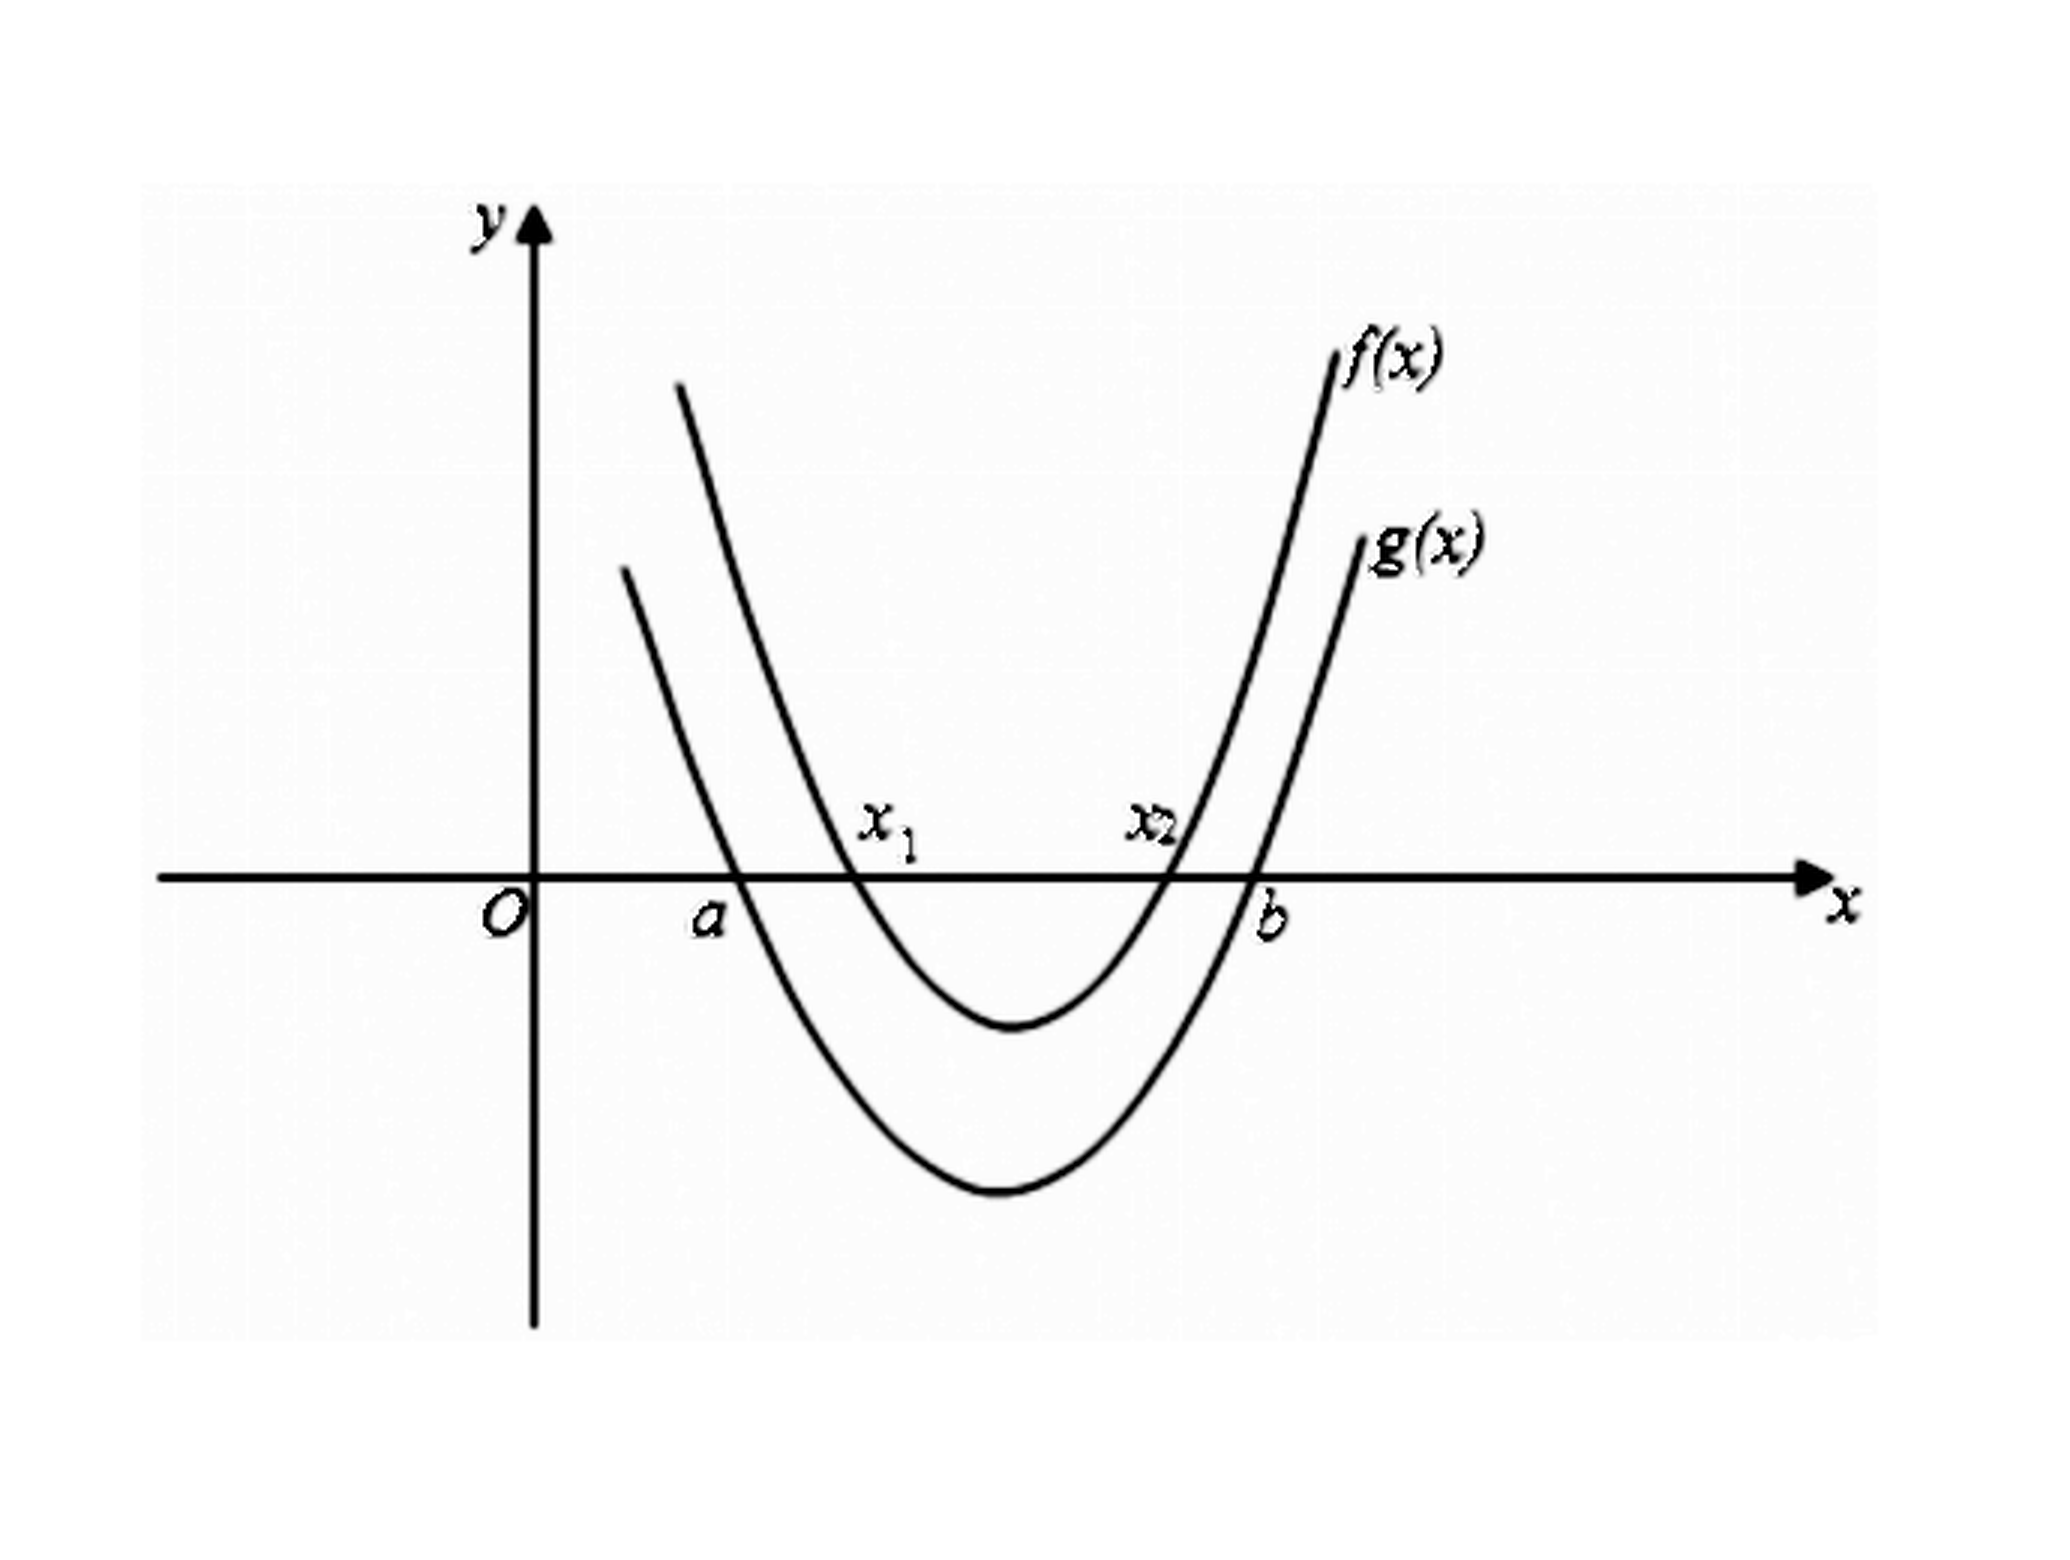
\includegraphics[width=0.52\textwidth]{figures/gao157_q16.png}
\end{center}

\step{由图像得 $a<x_1<x_2<b$，故选 $A$.}
\solend
\fi

\end{enumerate}

\bigsec{三、解答题}

\begin{enumerate}
\setcounter{enumi}{16}

% === Q17 === 解析 6 行；\overline{A}、\varnothing、\subseteq 无、cases
\item 设全集为 $\R$，$m\in\R$，集合 $A=\{x\mid 2<x<5\}$，$B=\{x\mid 2m\leqslant x\leqslant 5m-3\}$.

(1) 若 $m=2$，求 $\overline{A}\cup B$；

(2) 若 $A\cap B=B$，求 $m$ 的取值范围.

\ifanswer
\solbegin
\step{(1) $\overline{A}=\{x\mid x\leqslant2$ 或 $x\geqslant5\}$，当 $m=2$ 时，$B=\{x\mid 4\leqslant x\leqslant7\}$，}
\step{则 $\overline{A}\cup B=\{x\mid x\leqslant2$ 或 $x\geqslant4\}$；}
\step{(2) 因为 $A\cap B=B$，所以 $B$ 是 $A$ 的子集，}
\step{当 $B=\varnothing$ 时，$2m>5m-3$，解得 $m<1$；}
\step{当 $B\ne\varnothing$ 时，$\begin{cases}2m\leqslant5m-3\\2m>2\\5m-3<5\end{cases}$，解得 $1<m<\dfrac85$；}
\step{综上，$m$ 的取值范围是 $(-\infty,1)\cup\left(1,\dfrac85\right)$.}
\solend
\fi

% === Q18 === 解析 2 行；指数式、\lg、换底
\item (1) 设 $a^{2x}=3$，且 $a>0$，求 $\dfrac{a^{3x}+a^{-3x}}{a^x+a^{-x}}$ 的值；

(2) 已知 $\lg2=a, 10^b=3$，用 $a$ 及 $b$ 表示 $\log_{12}25$.

\ifanswer
\solbegin
\step{(1) $\dfrac{a^{3x}+a^{-3x}}{a^x+a^{-x}}=a^{2x}-1+a^{-2x}=3-1+\dfrac13=\dfrac73$；}
\step{(2) $\log_{12}25=\dfrac{\lg25}{\lg12}=\dfrac{2-2\lg2}{2\lg2+\lg3}=\dfrac{2-2a}{2a+b}$.}
\solend
\fi

% === Q19 === 解析 11 行；幂函数、$=0$ 笔误照录、\Delta、\sqrt5、cases
\item 已知幂函数 $f(x)=(m^2+m-1)x^{-2m^2+m+3}$ 在 $(0,+\infty)$ 上为严格增函数.

(1) 求 $f(x)$ 的解析式；

(2) 若 $k+kf(x)>f(x)-x-1$ 对任意实数 $x$ 都成立，求实数 $k$ 的取值范围；

(3) 若关于 $x$ 的不等式 $f(x)\leqslant8x-a$ 的解集中有且仅有 $5$ 个整数，求实数 $a$ 的范围.

\ifanswer
\solbegin
\step{(1) 由题意得 $m^2+m-1=1$，且 $-2m^2+m+3>0$，}
\step{解得 $m=-2$（舍去）或 $m=1$，所以 $f(x)=x^2$；}
\step{(2) $k+kf(x)>f(x)-x-1$ 可化为 $(k-1)x^2+x+k+1=0$ 恒成立，}
\step{当 $k=1$ 时，$x+2>0$，显然不恒成立；}
\step{当 $k\ne1$ 时，要使该二次不等式恒成立，只需 $\begin{cases}k-1>0\\[2pt]\Delta=1-4(k+1)(k-1)\leqslant0\end{cases}$，}
\step{解得 $k\geqslant\dfrac{\sqrt5}{2}$，即所求 $k$ 的范围是 $\left[\dfrac{\sqrt5}{2},+\infty\right)$；}
\step{(3) 不等式 $f(x)\leqslant8x-a$，即 $x^2-8x+a\leqslant0$ 有五个整数解，}
\step{令 $g(x)=x^2-8x+a$，因为该函数开口向上，对称轴为 $x=4$，}
\step{所以解集内的整数为 $2$，$3$，$4$，$5$，$6$，}
\step{由二次函数的性质得，只需 $\begin{cases}g(1)=1-8+a>0\\g(2)=4-8\times2+a\leqslant0\end{cases}$，解得 $7<a\leqslant12$，}
\step{故 $a$ 的取值范围是 $(7,12]$.}
\solend
\fi

% === Q20 === 解析 12 行；材料题、$a+b=1$、大根号、"因出"笔误、分母套分数
\item 问题：正数 $a$、$b$ 满足 $a+b=1$，求 $\dfrac1a+\dfrac2b$ 的最小值.

其中一种解法是：$\dfrac1a+\dfrac2b=\left(\dfrac1a+\dfrac2b\right)(a+b)=1+\dfrac ba+\dfrac{2a}{b}+2\geqslant3+2\sqrt2$，

当且仅当 $\dfrac ba=\dfrac{2a}{b}$ 且 $a+b=1$ 时，即 $a=\sqrt2-1$ 且 $b=2-\sqrt2$ 时取等号.

学习上述解法并解决下列问题：

(1) 若正实数 $x$、$y$ 满足 $x+y=1$，求 $\dfrac2x+\dfrac1y$ 的最小值；

(2) 若实数 $a$、$b$、$x$、$y$ 满足 $\dfrac{x^2}{a^2}-\dfrac{y^2}{b^2}=1$，求证：$a^2-b^2\leqslant(x-y)^2$；

(3) 利用 (2) 的结论，求代数式 $M=\sqrt{2m-5}-\sqrt{m-3}$ 的最小值，并求出使得 $M$ 最小的 $m$ 的值.

\ifanswer
\solbegin
\step{(1) $\dfrac2x+\dfrac1y=(x+y)\left(\dfrac2x+\dfrac1y\right)=3+\dfrac xy+\dfrac{2y}{x}\geqslant3+2\sqrt2$，}
\step{当且仅当 $\dfrac xy=\dfrac{2y}{x}$ 且 $x+y=1$ 时取等号；}
\step{(2) $a^2-b^2=(a^2-b^2)\left(\dfrac{x^2}{a^2}-\dfrac{y^2}{b^2}\right)=x^2+y^2-\left(\dfrac{a^2x^2}{b^2}+\dfrac{b^2y^2}{a^2}\right)$}
\step{$\leqslant x^2+y^2-2\sqrt{\dfrac{a^2x^2}{b^2}\cdot\dfrac{b^2y^2}{a^2}}=x^2+y^2-2xy=(x-y)^2$，}
\step{故当 $b^4x^2=a^4y^2$ 时，等号成立.}
\step{(3) 令 $x=\sqrt{2m-5}, y=\sqrt{m-3}$，由 $\begin{cases}2m-5\geqslant0\\m-3\geqslant0\end{cases}$ 得 $m\geqslant3$，}
\step{$x^2-y^2=(2m-5)-(m-3)=m-2>0$，}
\step{又 $x>0, y>0$，所以 $x>y$，所以 $\dfrac{x^2}{a^2}-\dfrac{y^2}{b^2}=1$，}
\step{由 $x^2-2y^2=1$，得 $\dfrac{x^2}{1}-\dfrac{y^2}{\frac12}=1$，因出 $a^2=1, b^2=\dfrac12$，}
\step{由 (2) 得 $M=\sqrt{2m-5}-\sqrt{m-3}=x-y\geqslant\sqrt{a^2-b^2}=\sqrt{1-\dfrac12}=\dfrac{\sqrt2}{2}$，}
\step{当且仅当 $\dfrac xy=\left(\dfrac ab\right)^2=2$ 取等号，结合 $x^2-2y^2=1$，解得 $x=\sqrt2, y=\dfrac{\sqrt2}{2}$，}
\step{即 $\sqrt{2m-5}=\sqrt2$，得 $m=\dfrac72$，所以 $m=\dfrac72$ 时，$M$ 取得最小值 $\dfrac{\sqrt2}{2}$.}
\solend
\fi

\end{enumerate}

\end{document}
"
% 紧凑版：xelatex "\def\iscompact{1}% 高一157_大境中学_期中.tex
%   —— 高一上数学"2026-2027 年大境中学高一上期中"（试卷版/答案版/紧凑版）
% 试卷版：xelatex 高一157_大境中学_期中.tex
% 答案版：xelatex "\def\isanswer{1}\input{高一157_大境中学_期中.tex}"
% 紧凑版：xelatex "\def\iscompact{1}\input{高一157_大境中学_期中.tex}"
%
% ① 原始材料：微信公众号"魔都数学加油站"文章，连载"27学年高一157"，原文标题
% "27学年高一157——2026-2027年上海市大境中学高一上期中"；
% 原文链接：https://mp.weixin.qq.com/s/s6eDMDVkxc2fcBe8LNm-Tw 。
% 正文为 8 张 PNG 页（01/02/03/04/06 为 4762×6735，05/07/08 为 2560×3620，
% 同一篇各页分辨率混排，逐页按各自分辨率裁图核对）。
% 体例：讲评版——填空 3—12（10 题）、选择 13—16（4 题）、解答 17—20（4 题），
% 共 18 题，自第 3 题起编（1、2 未印在本篇）；末题是第 20 题（不是 21）。
% 除第 4 题只印【答案】外，其余 17 题逐题印【解析】（逐题核实，见 ②）。
% 题目、答案、解析均据原图转录；卷面粉红色水印"魔都数学加油站"及公众号
% 页脚未录入。
% 全卷仅 1 幅配图：第 16 题解析内函数图像（"设 g(x)=(x-a)(x-b)，
% f(x)=g(x)+1，画出函数 g(x) 与函数 f(x) 的图像，如图所示"），
% 解析内配图仅答案版出，裁 figures/gao157_q16.png；逐页通读 8 页确认
% 无题目配图、无表格；08 页下半仅水印、无正文。
%
% 卷首标题：原卷印作"2026-2027 年大境中学高一上期中"，年份区间按全稿惯例排 en dash；
% 原卷卷面未印副标题，本稿按同期中卷知识模块口径补出"集合与常用逻辑用语、不等式、函数"。
%
% ② 与原卷的排版差异：
%   ① 原文从第 3 题起，本稿保留原题号；共 18 题三节，解答题 4 题到 20；
%      三节各自 \begin{enumerate}…\end{enumerate} + \setcounter{enumi}{2/12/16}
%      （题目溯源.py 按 \bigsec 切节、每节独立计 depth，只收 depth==1 的 \item，
%       见 高一156 头注②的订正）；
%   ② 第 4 题只印【答案】、无【解析】，提 \ans{}；其余 17 题逐题印【解析】、
%      逐题设 \solbegin…\solend；四道选择题答案在解析末句"故选 D／D／C／A"
%      （逐个放大复核）、括号 \mbox{（\quad）} 留空；答案版【答案】/【解析】
%      标记数 = 18 = 全卷题数（1 个 \ans ＋ 17 个 \solbegin）；
%   ③ 原卷卷面未印副标题，本稿按知识模块口径补出；
%   ④ 原卷填空横线按全稿惯例排 \blankline[4.4em]；选择题选项段前按惯例各加
%      \keepwithprev；解答题不留作答区、不加 \anspace（原卷为讲评版，109—113 起
%      全稿不用 \anspace）；
%   ⑤ 数集：Q4"$x、y\in R$"、Q6"$x\in R$"、Q10"$a\in Z$"、Q12"$n\in Z$"
%      "$n_1、n_2\in Z$"、Q17"全集为 R／$m\in R$"原卷印斜体 R/Z，按全稿惯例
%      归一 \R／\Z（参见 高一14 头注④、高一150 头注②⑤、高一153 头注⑤）；
%      绝对值排 \lvert…\rvert（Q6 $\lvert x-1\rvert$／$\lvert x+3\rvert$／
%      $\lvert 2x+2\rvert$），集合描述竖线排 \mid（Q12、Q17），空集 \varnothing
%      （Q17"$B=\varnothing$"），补集照原卷上划线排 \overline{A}（Q17），
%      不等号按全稿惯例排 \leqslant／\geqslant；
%   ⑥ 判别式三处（Q8"$\Delta=(-2m)^2-4(m+2)$"、Q15"$\Delta=(a+2)^2+4(a^2-4)<0$"、
%      Q19"$\Delta=1-4(k+1)(k-1)\leqslant0$"）放大比对同形、均为等腰偏高且右斜边
%      加粗的 \Delta，统一照录 \Delta；本卷无扁三角 \triangle 用例（与 高一142／
%      高一151／高一152 的 Δ/△ 混用卷不同）；
%   ⑦ "图像／图象"逐处照录不统一：Q9"图像过点 $(4,2)$""它的图像过点"、
%      Q16"画出函数 $g(x)$ 与函数 $f(x)$ 的图像""由图像得"用"图像"；
%      Q14 题干及解析四处均用"图象"（"的图象关于原点对称""图象关于 $y$ 轴对称"）；
%   ⑧ 原卷笔误／未化简式照录：
%      · Q5 解析"$2\sqrt4+1=5$"根号 4 原卷未化简，照录 \sqrt4；
%      · Q7 解析"$\lg\frac{E_1}{E_2}=\frac25\cdot(m_2-m_1)=\frac25(-1.45+26.7)=10.1$"
%        第一处有 \cdot、第二处无，逐处照录；题干"$m_1-m_2=-\frac52\lg\frac{E_1}{E_2}$"；
%      · Q10 解析"$f(1)=\frac{a+1}{1+2}\geqslant0$"与 cases 第二行分母均印 $1+2$、
%        未化简成 $3$，照录；
%      · Q19 (2)"可化为 $(k-1)x^2+x+k+1=0$ 恒成立"原卷印 $=0$（与 >0 恒成立
%        的题意不符），照录笔误；
%      · Q20 (3)"因出 $a^2=1, b^2=\frac12$"原卷印"因出"（当作"因此"），照录；
%      · Q20 (3)"得 $\frac{x^2}{1}-\frac{y^2}{\frac12}=1$"分母套分数、照录；
%   ⑨ 圈数字①②在文本模式（Q15 解析"①当 $a^2-4=0$ 时""②当 $a^2-4\ne0$ 时"，
%      共 2 枚）；子题标号 (1)(2)(3) 半角括号照录；行末西文句点 ASCII `.`；
%      行中全角逗号／顿号照录；半角逗号在数学组之间是全稿惯例、非笔误
%      （Q8"$x_1+x_2=2m, x_1x_2=m+2$"、Q12"$n\in Z$"、Q18"$\lg2=a, 10^b=3$"、
%      Q20"$a^2=1, b^2=\frac12$"等）；中文弯引号""照录（Q4 命题）；
%   ⑩ 自定义名词：Q11"交叉数"、Q12"$a\otimes b$"新定义运算、Q20"问题／
%      其中一种解法是／学习上述解法并解决下列问题"材料题，均照原卷录入；
%   ⑪ 配图：全卷 1 幅（逐页通读 8 页确认）——Q16 解析内函数图像（05 页右侧，
%      $f(x)$ 与 $g(x)$ 两条抛物线、标注 $a,x_1,x_2,b$），仅答案版出，
%      裁 figures/gao157_q16.png，去粉色水印、去色、3× LANCZOS 放大；
%      图放 \ifanswer 内 \solbegin…\solend 的两 \step 之间（高一108 第 6 题／
%      高一156 Q15 成例）；Q16 题干无"如图"、不需题目配图守卫。
%
% ③ 行数复核：一条 \step = 原卷解析的一个印刷行，cases 块作一个印刷行计；
%    跨半页重叠行（Q5 的"【解析】x-1>0…"、Q10 的"所以 a=-1 或 a=0"、
%    Q12 的"【解析】由 u⊗v…"、Q14 的"f(x)=x² 图象关于 y 轴对称"、
%    Q19 的"(1) 由题意得…"、Q20 的"(3) 令 x=…"等 hi_1/hi_2 两半页共有的行）
%    只计一次，别把原卷折行并起来。
%    逐题数（主会话逐页核对定稿）：Q3：1；Q4：0（只印【答案】、提 \ans{}，
%    不计入 \step 账）；Q5：2；Q6：5；Q7：2；Q8：5；Q9：3；Q10：4；
%    Q11：3；Q12：6；Q13：3；Q14：5；Q15：9；Q16：4；Q17：6；Q18：2；
%    Q19：11；Q20：12。合计 83 条 \step（本卷无 \stepm），与原卷逐题印刷行相等。
%    全卷 18 题：1 题只印【答案】（\ans）、17 题印【解析】（\solbegin…\solend），
%    答案版【答案】/【解析】标记数 = 18 = 全卷题数。
%    全卷除此 6 类外未发现其它笔误／自相矛盾处；17 题印【解析】、1 题印【答案】。
%
\documentclass[a4paper,11pt]{article}
\usepackage{common}

\begin{document}

\examtitlest[3]{2026--2027 年大境中学高一上期中}{集合与常用逻辑用语、不等式、函数}

\bigsec{一、填空题}

\begin{enumerate}
\setcounter{enumi}{2}

% === Q3 === 解析 1 行；$a,b$ 半角逗号照录
\item 若 $a=x^2-2x+1$，$b=x-3$，则 $a,b$ 的大小关系为\blankline[4.4em].

\ifanswer
\solbegin
\step{$a-b=x^2-3x+4=\left(x-\dfrac32\right)^2+\dfrac74>0$，所以 $a>b$.}
\solend
\fi

% === Q4 === 只印【答案】、无【解析】；中文弯引号、\R、顿号；提 \ans{}
\item 用反证法证明命题：“设 $x$、$y\in\R$. 若 $x+y>2$，则 $x>1$ 或 $y>1$”时，假设的内容应该是\blankline[4.4em].

\ifanswer
\ans{$x\leqslant1$ 且 $y\leqslant1$}
\fi

% === Q5 === 解析 2 行；$2\sqrt4+1=5$ 根号 4 未化简照录
\item 当 $x>1$ 时，$x+\dfrac4{x-1}$ 的最小值为\blankline[4.4em].

\ifanswer
\solbegin
\step{$x-1>0$，$x+\dfrac4{x-1}=(x-1)+\dfrac4{x-1}+1\geqslant2\sqrt4+1=5$，}
\step{当且仅当 $x-1=\dfrac4{x-1}$，即 $x=3$ 时取等号，故最小值为 $5$.}
\solend
\fi

% === Q6 === 解析 5 行；绝对值 \lvert…\rvert、\cup、\R
\item 设 $x\in\R$，方程 $\lvert x-1\rvert+\lvert x+3\rvert=\lvert 2x+2\rvert$ 的解集是\blankline[4.4em].

\ifanswer
\solbegin
\step{当 $x\leqslant-3$ 时，方程为 $1-x-x-3=-2x-2$，等式成立；}
\step{当 $-3<x\leqslant-1$ 时，方程为 $1-x+x+3=-2x-2$，解得 $x=-3$，舍去；}
\step{当 $-1<x<1$ 时，方程为 $1-x+x+3=2x+2$，解得 $x=1$，舍去；}
\step{当 $x\geqslant1$ 时，方程为 $x-1+x+3=2x+2$，等式成立，}
\step{综上，方程 $\lvert x-1\rvert+\lvert x+3\rvert=\lvert 2x+2\rvert$ 的解集为 $(-\infty,-3]\cup[1,+\infty)$.}
\solend
\fi

% === Q7 === 解析 2 行；星等材料题、\lg、\cdot 逐处照录、天狼星
\item 在天文学中，天体的明暗程度可以用星等或亮度来描述，两颗星的星等与亮度满足 $m_1-m_2=-\dfrac52\lg\dfrac{E_1}{E_2}$，其中星等为 $m_k$ 的星的亮度为 $E_k(k=1,2)$. 已知太阳的星等为 $-26.7$，天狼星的星等为 $-1.45$，则太阳与天狼星的亮度的比值为\blankline[4.4em].

\ifanswer
\solbegin
\step{两颗星的星等与亮度满足 $m_1-m_2=-\dfrac52\lg\dfrac{E_1}{E_2}$，令 $m_2=-1.45$，$m_1=-26.7$，}
\step{$\lg\dfrac{E_1}{E_2}=\dfrac25\cdot(m_2-m_1)=\dfrac25(-1.45+26.7)=10.1$，$\dfrac{E_1}{E_2}=10^{10.1}$.}
\solend
\fi

% === Q8 === 解析 5 行；韦达定理、判别式 \Delta、半角逗号在数学组间
\item 已知方程 $x^2-2mx+m+2=0$ 有两个实数根 $x_1,x_2$，满足 $x_1^2+x_2^2=2$，则实数 $m$ 的值为\blankline[4.4em].

\ifanswer
\solbegin
\step{对于方程 $x^2-2mx+m+2=0$，由韦达定理得 $x_1+x_2=2m, x_1x_2=m+2$，}
\step{又 $x_1^2+x_2^2=(x_1+x_2)^2-2x_1x_2=(2m)^2-2(m+2)=4m^2-2m-4=2$，}
\step{解得 $m=\dfrac32$ 或 $m=-1$，}
\step{因为方程有两个实数根，所以 $\Delta=(-2m)^2-4(m+2)=4m^2-4m-8\geqslant0$，}
\step{解得 $m\leqslant-1$ 或 $m\geqslant2$，故 $m=-1$.}
\solend
\fi

% === Q9 === 解析 3 行；"图像"照录、$x^\alpha$、$x^{1/2}=\sqrt{x}$
\item 已知幂函数 $y=f(x)$ 的图像过点 $(4,2)$，则不等式 $f(x^2-2x)<f(2-x)$ 的解集为\blankline[4.4em].

\ifanswer
\solbegin
\step{设幂函数 $y=f(x)=x^\alpha$，它的图像过点 $(4,2)$，所以 $4^\alpha=2$，$\alpha=\dfrac12$，}
\step{故 $f(x)=x^{\frac12}=\sqrt{x}$，由不等式 $f(x^2-2x)<f(2-x)$，}
\step{得 $0\leqslant x^2-2x<2-x$，得 $-1<x\leqslant0$，故解集为 $(-1,0]$.}
\solend
\fi

% === Q10 === 解析 4 行；$a\in\Z$、cases（分母 $1+2$ 未化简）、参数分离
\item 已知函数 $y=\dfrac{ax+1}{x+2}$（常数 $a\in\Z$）. 要使该函数在区间 $[1,+\infty)$ 上是严格减函数，并且函数值不恒为负，则满足条件的 $a$ 的取值为\blankline[4.4em].

\ifanswer
\solbegin
\step{函数参数分离为 $y=\dfrac{a(x+2)+1-2a}{x+2}=a+\dfrac{1-2a}{x+2}$，}
\step{若函数在区间 $[1,+\infty)$ 上严格减函数，则 $1-2a>0$，}
\step{且函数的最大值 $f(1)=\dfrac{a+1}{1+2}\geqslant0$，即 $\begin{cases}1-2a>0\\[2pt]\dfrac{a+1}{1+2}\geqslant0\end{cases}$，解得 $-1\leqslant a<\dfrac12$，又 $a\in\Z$，}
\step{所以 $a=-1$ 或 $a=0$.}
\solend
\fi

% === Q11 === 解析 3 行；"交叉数"自定义名词、$(-1)^t$、$2^5$、$32\times3=96$
\item 对非空集合 $A$ 中的每个元素 $t$，都乘以 $(-1)^t$ 再求和，称为集合 $A$ 的交叉数，例如 $A=\{2,3,6\}$，则集合 $A$ 的交叉数为 $(-1)^2\cdot2+(-1)^3\cdot3+(-1)^6\cdot6=5$. 若集合 $W=\{1,2,3,4,5,6\}$，则 $W$ 的所有非空子集的交叉数的总和为\blankline[4.4em].

\ifanswer
\solbegin
\step{固定 $W$ 中的任一元素，其余 $5$ 个元素各有选或不选两种情况，}
\step{因此该元素出现在 $2^5$ 个非空子集中，}
\step{所有交叉数的总和为 $2^5(-1+2-3+4-5+6)=32\times3=96$.}
\solend
\fi

% === Q12 === 解析 6 行；\otimes、\lambda、\mid、\Z、\times 与 \cdot 逐处照录
\item 对于任意两个正实数 $a$、$b$，定义 $a\otimes b=\lambda\cdot\dfrac ab$，其中常数 $\lambda\in\left(\dfrac{\sqrt2}{2},1\right)$. 若 $u\geqslant v>0$，且 $u\otimes v$ 与 $v\otimes u$ 都是集合 $\left\{x\mid x=\dfrac n2,n\in\Z\right\}$ 的元素，则 $u\otimes v=$\blankline[4.4em].

\ifanswer
\solbegin
\step{由 $u\otimes v$ 与 $v\otimes u$ 都是集合 $\left\{x\mid x=\dfrac n2,n\in\Z\right\}$ 的元素，}
\step{不妨设 $\lambda\times\dfrac uv=\dfrac12 n_1$，$\lambda\times\dfrac vu=\dfrac12 n_2$，$n_1$、$n_2\in\Z$，}
\step{因为 $u\geqslant v>0$，所以 $0<\dfrac vu\leqslant1$，因为 $\lambda\in\left(\dfrac{\sqrt2}{2},1\right)$，所以 $\dfrac12 n_2=\lambda\cdot\dfrac vu\in(0,1)$，}
\step{因为 $n_2\in\Z$，所以 $n_2=1$，即 $\dfrac12=\dfrac{\lambda v}{u}$，所以 $\lambda=\dfrac{u}{2v}\in\left(\dfrac{\sqrt2}{2},1\right)$，}
\step{所以 $\dfrac uv\in(\sqrt2,2)$，$\dfrac{u^2}{v^2}\in(2,4)$，则 $\lambda\cdot\dfrac uv=\dfrac{u^2}{v^2}\times\dfrac12=\dfrac12 n_1\in(1,2)$，}
\step{因为 $n_1\in\Z$，所以 $n_1=3$，$\dfrac12 n_1=\dfrac32$，故 $u\otimes v=\dfrac32$.}
\solend
\fi

\end{enumerate}

\bigsec{二、选择题}

\begin{enumerate}
\setcounter{enumi}{12}

% === Q13 === 解析 3 行；选项段 \keepwithprev；故选 D
\item 下列不等式成立的为\mbox{（\quad）}

\keepwithprev
A. 若 $a>b$，则 $ac^2>bc^2$\qquad B. 若 $a>b$，则 $a^2>b^2$

C. 若 $a>b$，$c>d$，则 $a+b>c+d$\qquad D. 若 $a>b$，则 $a^3>b^3$

\ifanswer
\solbegin
\step{A 中 $c=0$ 时不成立；B 取 $a=1$，$b=-2$ 不成立；}
\step{C 取 $a=1$，$b=0$，$c=5$，$d=0$ 不成立.}
\step{幂函数 $y=x^3$ 在实数集上严格递增，所以 $a>b\Rightarrow a^3>b^3$，故选 $D$.}
\solend
\fi

% === Q14 === 解析 5 行；"图象"四处照录；故选 D
\item 幂函数 $f(x)=x^\alpha$ 的图象关于原点对称，且在 $(-\infty,0)$ 上是严格增函数，则 $f(x)$ 可以是\mbox{（\quad）}

\keepwithprev
A. $f(x)=x^{-1}$\qquad B. $f(x)=x^{\frac12}$\qquad C. $f(x)=x^2$\qquad D. $f(x)=x^3$

\ifanswer
\solbegin
\step{$f(x)=\dfrac1x$ 的图象关于原点对称，在 $(-\infty,0)$ 上是严格减函数，故 $A$ 错误；}
\step{$f(x)=x^{\frac12}$ 在 $(-\infty,0)$ 上无意义，故 $B$ 错误；}
\step{$f(x)=x^2$ 图象关于 $y$ 轴对称，故 $C$ 错误；}
\step{$f(x)=x^3$ 的图象关于原点对称，且在 $(-\infty,0)$ 上是严格增函数，故 $D$ 正确.}
\step{故选 $D$.}
\solend
\fi

% === Q15 === 解析 9 行；圈数字①②、\Delta、cases；故选 C
\item 若关于 $x$ 的不等式 $(a^2-4)x^2+(a+2)x-1\geqslant0$ 的解集不为空集，则实数 $a$ 的取值范围为\mbox{（\quad）}

\keepwithprev
A. $\left(-2,\dfrac65\right]$\qquad B. $\left[-2,\dfrac65\right]$

C. $(-\infty,-2)\cup\left[\dfrac65,+\infty\right)$\qquad D. $(-\infty,-2]\cup\left[\dfrac65,+\infty\right)$

\ifanswer
\solbegin
\step{①当 $a^2-4=0$ 时，$a=\pm2$，}
\step{若 $a=2$ 时，原不等式为 $4x-1\geqslant0$，则不等式的解集不是空集；}
\step{若 $a=-2$ 时，原不等式为 $-1\geqslant0$，无解，不符合题意；}
\step{②当 $a^2-4\ne0$ 时，$a\ne\pm2$，}
\step{若 $(a^2-4)x^2+(a+2)x-1\geqslant0$ 的解集是空集，则 $\begin{cases}a^2-4<0\\[2pt]\Delta=(a+2)^2+4(a^2-4)<0\end{cases}$，}
\step{解得 $-2<a<\dfrac65$，}
\step{则当不等式 $(a^2-4)x^2+(a+2)x-1\geqslant0$ 的解集不为空集时，}
\step{有 $a<-2$ 或 $a\geqslant\dfrac65$ 且 $a\ne2$，}
\step{综上，实数 $a$ 的取值范围为 $(-\infty,-2)\cup\left[\dfrac65,+\infty\right)$，故选 $C$.}
\solend
\fi

% === Q16 === 解析 4 行＋1 幅解析内配图（仅答案版）；"图像"照录；故选 A
\item 已知实数 $a<b$，关于 $x$ 的不等式 $x^2-(a+b)x+ab+1<0$ 的解集为 $(x_1,x_2)$，则实数 $a$、$b$、$x_1$、$x_2$ 从小到大的排列是\mbox{（\quad）}

\keepwithprev
A. $a<x_1<x_2<b$\qquad B. $x_1<a<b<x_2$\qquad C. $a<x_1<b<x_2$\qquad D. $x_1<a<x_2<b$

\ifanswer
\solbegin
\step{不等式 $x^2-(a+b)x+ab+1<0$ 可化为 $(x-a)(x-b)+1<0$，}
\step{设 $g(x)=(x-a)(x-b)$，$f(x)=g(x)+1$，}
\step{画出函数 $g(x)$ 与函数 $f(x)$ 的图像，如图所示，}

\begin{center}
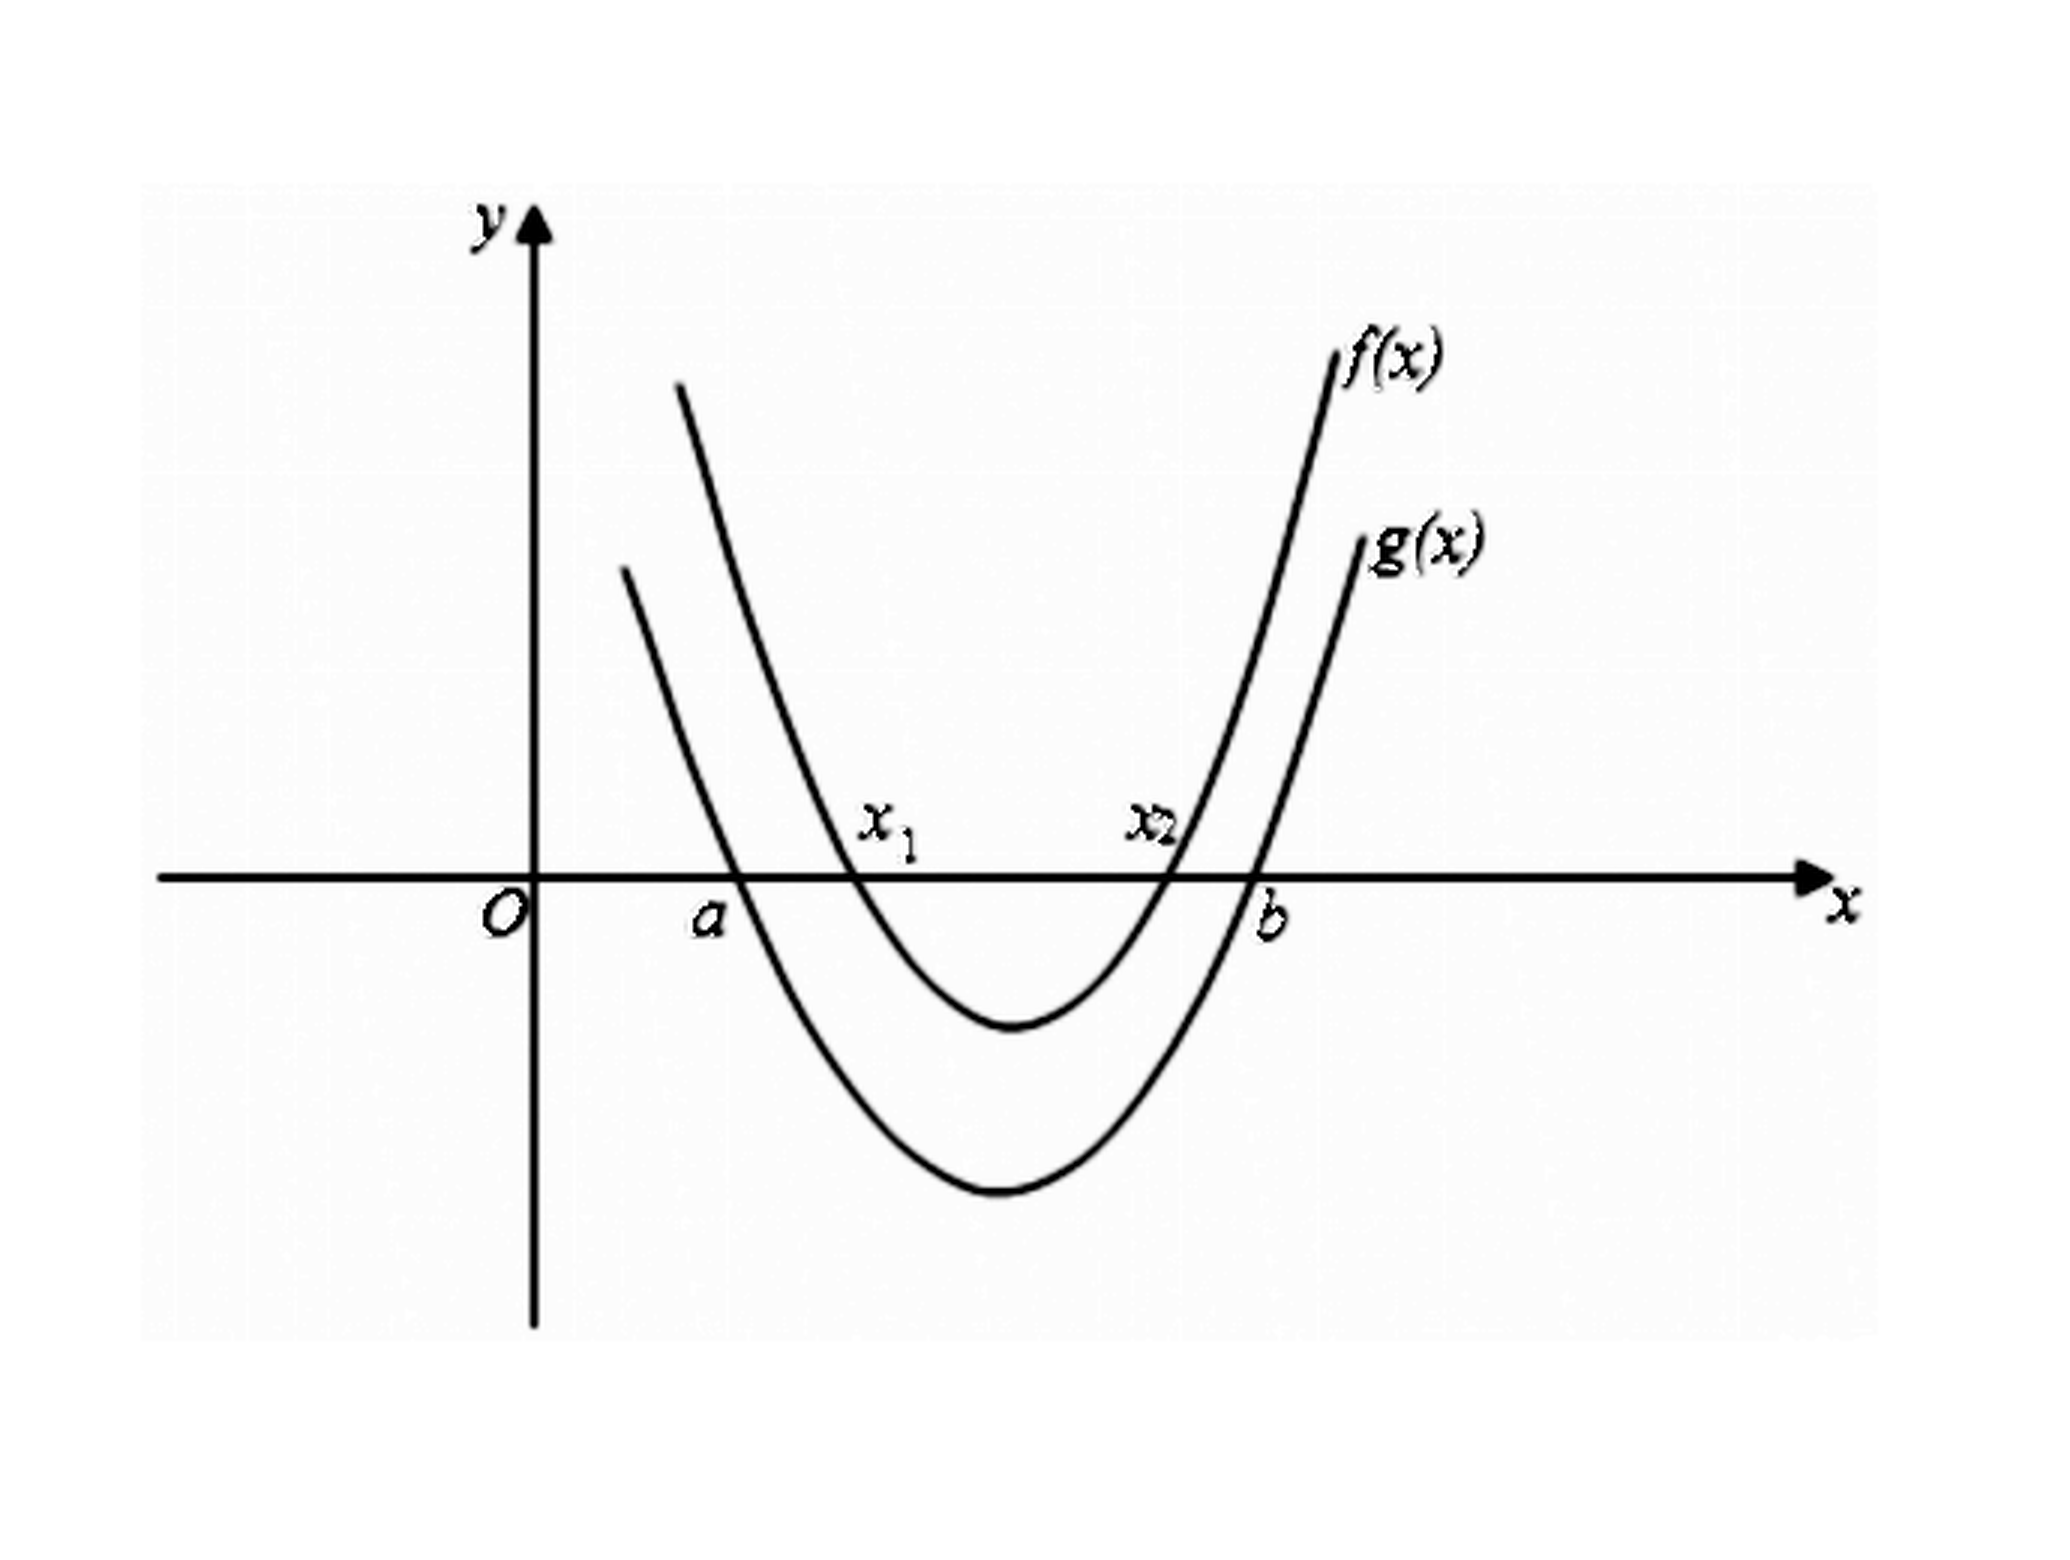
\includegraphics[width=0.52\textwidth]{figures/gao157_q16.png}
\end{center}

\step{由图像得 $a<x_1<x_2<b$，故选 $A$.}
\solend
\fi

\end{enumerate}

\bigsec{三、解答题}

\begin{enumerate}
\setcounter{enumi}{16}

% === Q17 === 解析 6 行；\overline{A}、\varnothing、\subseteq 无、cases
\item 设全集为 $\R$，$m\in\R$，集合 $A=\{x\mid 2<x<5\}$，$B=\{x\mid 2m\leqslant x\leqslant 5m-3\}$.

(1) 若 $m=2$，求 $\overline{A}\cup B$；

(2) 若 $A\cap B=B$，求 $m$ 的取值范围.

\ifanswer
\solbegin
\step{(1) $\overline{A}=\{x\mid x\leqslant2$ 或 $x\geqslant5\}$，当 $m=2$ 时，$B=\{x\mid 4\leqslant x\leqslant7\}$，}
\step{则 $\overline{A}\cup B=\{x\mid x\leqslant2$ 或 $x\geqslant4\}$；}
\step{(2) 因为 $A\cap B=B$，所以 $B$ 是 $A$ 的子集，}
\step{当 $B=\varnothing$ 时，$2m>5m-3$，解得 $m<1$；}
\step{当 $B\ne\varnothing$ 时，$\begin{cases}2m\leqslant5m-3\\2m>2\\5m-3<5\end{cases}$，解得 $1<m<\dfrac85$；}
\step{综上，$m$ 的取值范围是 $(-\infty,1)\cup\left(1,\dfrac85\right)$.}
\solend
\fi

% === Q18 === 解析 2 行；指数式、\lg、换底
\item (1) 设 $a^{2x}=3$，且 $a>0$，求 $\dfrac{a^{3x}+a^{-3x}}{a^x+a^{-x}}$ 的值；

(2) 已知 $\lg2=a, 10^b=3$，用 $a$ 及 $b$ 表示 $\log_{12}25$.

\ifanswer
\solbegin
\step{(1) $\dfrac{a^{3x}+a^{-3x}}{a^x+a^{-x}}=a^{2x}-1+a^{-2x}=3-1+\dfrac13=\dfrac73$；}
\step{(2) $\log_{12}25=\dfrac{\lg25}{\lg12}=\dfrac{2-2\lg2}{2\lg2+\lg3}=\dfrac{2-2a}{2a+b}$.}
\solend
\fi

% === Q19 === 解析 11 行；幂函数、$=0$ 笔误照录、\Delta、\sqrt5、cases
\item 已知幂函数 $f(x)=(m^2+m-1)x^{-2m^2+m+3}$ 在 $(0,+\infty)$ 上为严格增函数.

(1) 求 $f(x)$ 的解析式；

(2) 若 $k+kf(x)>f(x)-x-1$ 对任意实数 $x$ 都成立，求实数 $k$ 的取值范围；

(3) 若关于 $x$ 的不等式 $f(x)\leqslant8x-a$ 的解集中有且仅有 $5$ 个整数，求实数 $a$ 的范围.

\ifanswer
\solbegin
\step{(1) 由题意得 $m^2+m-1=1$，且 $-2m^2+m+3>0$，}
\step{解得 $m=-2$（舍去）或 $m=1$，所以 $f(x)=x^2$；}
\step{(2) $k+kf(x)>f(x)-x-1$ 可化为 $(k-1)x^2+x+k+1=0$ 恒成立，}
\step{当 $k=1$ 时，$x+2>0$，显然不恒成立；}
\step{当 $k\ne1$ 时，要使该二次不等式恒成立，只需 $\begin{cases}k-1>0\\[2pt]\Delta=1-4(k+1)(k-1)\leqslant0\end{cases}$，}
\step{解得 $k\geqslant\dfrac{\sqrt5}{2}$，即所求 $k$ 的范围是 $\left[\dfrac{\sqrt5}{2},+\infty\right)$；}
\step{(3) 不等式 $f(x)\leqslant8x-a$，即 $x^2-8x+a\leqslant0$ 有五个整数解，}
\step{令 $g(x)=x^2-8x+a$，因为该函数开口向上，对称轴为 $x=4$，}
\step{所以解集内的整数为 $2$，$3$，$4$，$5$，$6$，}
\step{由二次函数的性质得，只需 $\begin{cases}g(1)=1-8+a>0\\g(2)=4-8\times2+a\leqslant0\end{cases}$，解得 $7<a\leqslant12$，}
\step{故 $a$ 的取值范围是 $(7,12]$.}
\solend
\fi

% === Q20 === 解析 12 行；材料题、$a+b=1$、大根号、"因出"笔误、分母套分数
\item 问题：正数 $a$、$b$ 满足 $a+b=1$，求 $\dfrac1a+\dfrac2b$ 的最小值.

其中一种解法是：$\dfrac1a+\dfrac2b=\left(\dfrac1a+\dfrac2b\right)(a+b)=1+\dfrac ba+\dfrac{2a}{b}+2\geqslant3+2\sqrt2$，

当且仅当 $\dfrac ba=\dfrac{2a}{b}$ 且 $a+b=1$ 时，即 $a=\sqrt2-1$ 且 $b=2-\sqrt2$ 时取等号.

学习上述解法并解决下列问题：

(1) 若正实数 $x$、$y$ 满足 $x+y=1$，求 $\dfrac2x+\dfrac1y$ 的最小值；

(2) 若实数 $a$、$b$、$x$、$y$ 满足 $\dfrac{x^2}{a^2}-\dfrac{y^2}{b^2}=1$，求证：$a^2-b^2\leqslant(x-y)^2$；

(3) 利用 (2) 的结论，求代数式 $M=\sqrt{2m-5}-\sqrt{m-3}$ 的最小值，并求出使得 $M$ 最小的 $m$ 的值.

\ifanswer
\solbegin
\step{(1) $\dfrac2x+\dfrac1y=(x+y)\left(\dfrac2x+\dfrac1y\right)=3+\dfrac xy+\dfrac{2y}{x}\geqslant3+2\sqrt2$，}
\step{当且仅当 $\dfrac xy=\dfrac{2y}{x}$ 且 $x+y=1$ 时取等号；}
\step{(2) $a^2-b^2=(a^2-b^2)\left(\dfrac{x^2}{a^2}-\dfrac{y^2}{b^2}\right)=x^2+y^2-\left(\dfrac{a^2x^2}{b^2}+\dfrac{b^2y^2}{a^2}\right)$}
\step{$\leqslant x^2+y^2-2\sqrt{\dfrac{a^2x^2}{b^2}\cdot\dfrac{b^2y^2}{a^2}}=x^2+y^2-2xy=(x-y)^2$，}
\step{故当 $b^4x^2=a^4y^2$ 时，等号成立.}
\step{(3) 令 $x=\sqrt{2m-5}, y=\sqrt{m-3}$，由 $\begin{cases}2m-5\geqslant0\\m-3\geqslant0\end{cases}$ 得 $m\geqslant3$，}
\step{$x^2-y^2=(2m-5)-(m-3)=m-2>0$，}
\step{又 $x>0, y>0$，所以 $x>y$，所以 $\dfrac{x^2}{a^2}-\dfrac{y^2}{b^2}=1$，}
\step{由 $x^2-2y^2=1$，得 $\dfrac{x^2}{1}-\dfrac{y^2}{\frac12}=1$，因出 $a^2=1, b^2=\dfrac12$，}
\step{由 (2) 得 $M=\sqrt{2m-5}-\sqrt{m-3}=x-y\geqslant\sqrt{a^2-b^2}=\sqrt{1-\dfrac12}=\dfrac{\sqrt2}{2}$，}
\step{当且仅当 $\dfrac xy=\left(\dfrac ab\right)^2=2$ 取等号，结合 $x^2-2y^2=1$，解得 $x=\sqrt2, y=\dfrac{\sqrt2}{2}$，}
\step{即 $\sqrt{2m-5}=\sqrt2$，得 $m=\dfrac72$，所以 $m=\dfrac72$ 时，$M$ 取得最小值 $\dfrac{\sqrt2}{2}$.}
\solend
\fi

\end{enumerate}

\end{document}
"
%
% ① 原始材料：微信公众号"魔都数学加油站"文章，连载"27学年高一157"，原文标题
% "27学年高一157——2026-2027年上海市大境中学高一上期中"；
% 原文链接：https://mp.weixin.qq.com/s/s6eDMDVkxc2fcBe8LNm-Tw 。
% 正文为 8 张 PNG 页（01/02/03/04/06 为 4762×6735，05/07/08 为 2560×3620，
% 同一篇各页分辨率混排，逐页按各自分辨率裁图核对）。
% 体例：讲评版——填空 3—12（10 题）、选择 13—16（4 题）、解答 17—20（4 题），
% 共 18 题，自第 3 题起编（1、2 未印在本篇）；末题是第 20 题（不是 21）。
% 除第 4 题只印【答案】外，其余 17 题逐题印【解析】（逐题核实，见 ②）。
% 题目、答案、解析均据原图转录；卷面粉红色水印"魔都数学加油站"及公众号
% 页脚未录入。
% 全卷仅 1 幅配图：第 16 题解析内函数图像（"设 g(x)=(x-a)(x-b)，
% f(x)=g(x)+1，画出函数 g(x) 与函数 f(x) 的图像，如图所示"），
% 解析内配图仅答案版出，裁 figures/gao157_q16.png；逐页通读 8 页确认
% 无题目配图、无表格；08 页下半仅水印、无正文。
%
% 卷首标题：原卷印作"2026-2027 年大境中学高一上期中"，年份区间按全稿惯例排 en dash；
% 原卷卷面未印副标题，本稿按同期中卷知识模块口径补出"集合与常用逻辑用语、不等式、函数"。
%
% ② 与原卷的排版差异：
%   ① 原文从第 3 题起，本稿保留原题号；共 18 题三节，解答题 4 题到 20；
%      三节各自 \begin{enumerate}…\end{enumerate} + \setcounter{enumi}{2/12/16}
%      （题目溯源.py 按 \bigsec 切节、每节独立计 depth，只收 depth==1 的 \item，
%       见 高一156 头注②的订正）；
%   ② 第 4 题只印【答案】、无【解析】，提 \ans{}；其余 17 题逐题印【解析】、
%      逐题设 \solbegin…\solend；四道选择题答案在解析末句"故选 D／D／C／A"
%      （逐个放大复核）、括号 \mbox{（\quad）} 留空；答案版【答案】/【解析】
%      标记数 = 18 = 全卷题数（1 个 \ans ＋ 17 个 \solbegin）；
%   ③ 原卷卷面未印副标题，本稿按知识模块口径补出；
%   ④ 原卷填空横线按全稿惯例排 \blankline[4.4em]；选择题选项段前按惯例各加
%      \keepwithprev；解答题不留作答区、不加 \anspace（原卷为讲评版，109—113 起
%      全稿不用 \anspace）；
%   ⑤ 数集：Q4"$x、y\in R$"、Q6"$x\in R$"、Q10"$a\in Z$"、Q12"$n\in Z$"
%      "$n_1、n_2\in Z$"、Q17"全集为 R／$m\in R$"原卷印斜体 R/Z，按全稿惯例
%      归一 \R／\Z（参见 高一14 头注④、高一150 头注②⑤、高一153 头注⑤）；
%      绝对值排 \lvert…\rvert（Q6 $\lvert x-1\rvert$／$\lvert x+3\rvert$／
%      $\lvert 2x+2\rvert$），集合描述竖线排 \mid（Q12、Q17），空集 \varnothing
%      （Q17"$B=\varnothing$"），补集照原卷上划线排 \overline{A}（Q17），
%      不等号按全稿惯例排 \leqslant／\geqslant；
%   ⑥ 判别式三处（Q8"$\Delta=(-2m)^2-4(m+2)$"、Q15"$\Delta=(a+2)^2+4(a^2-4)<0$"、
%      Q19"$\Delta=1-4(k+1)(k-1)\leqslant0$"）放大比对同形、均为等腰偏高且右斜边
%      加粗的 \Delta，统一照录 \Delta；本卷无扁三角 \triangle 用例（与 高一142／
%      高一151／高一152 的 Δ/△ 混用卷不同）；
%   ⑦ "图像／图象"逐处照录不统一：Q9"图像过点 $(4,2)$""它的图像过点"、
%      Q16"画出函数 $g(x)$ 与函数 $f(x)$ 的图像""由图像得"用"图像"；
%      Q14 题干及解析四处均用"图象"（"的图象关于原点对称""图象关于 $y$ 轴对称"）；
%   ⑧ 原卷笔误／未化简式照录：
%      · Q5 解析"$2\sqrt4+1=5$"根号 4 原卷未化简，照录 \sqrt4；
%      · Q7 解析"$\lg\frac{E_1}{E_2}=\frac25\cdot(m_2-m_1)=\frac25(-1.45+26.7)=10.1$"
%        第一处有 \cdot、第二处无，逐处照录；题干"$m_1-m_2=-\frac52\lg\frac{E_1}{E_2}$"；
%      · Q10 解析"$f(1)=\frac{a+1}{1+2}\geqslant0$"与 cases 第二行分母均印 $1+2$、
%        未化简成 $3$，照录；
%      · Q19 (2)"可化为 $(k-1)x^2+x+k+1=0$ 恒成立"原卷印 $=0$（与 >0 恒成立
%        的题意不符），照录笔误；
%      · Q20 (3)"因出 $a^2=1, b^2=\frac12$"原卷印"因出"（当作"因此"），照录；
%      · Q20 (3)"得 $\frac{x^2}{1}-\frac{y^2}{\frac12}=1$"分母套分数、照录；
%   ⑨ 圈数字①②在文本模式（Q15 解析"①当 $a^2-4=0$ 时""②当 $a^2-4\ne0$ 时"，
%      共 2 枚）；子题标号 (1)(2)(3) 半角括号照录；行末西文句点 ASCII `.`；
%      行中全角逗号／顿号照录；半角逗号在数学组之间是全稿惯例、非笔误
%      （Q8"$x_1+x_2=2m, x_1x_2=m+2$"、Q12"$n\in Z$"、Q18"$\lg2=a, 10^b=3$"、
%      Q20"$a^2=1, b^2=\frac12$"等）；中文弯引号""照录（Q4 命题）；
%   ⑩ 自定义名词：Q11"交叉数"、Q12"$a\otimes b$"新定义运算、Q20"问题／
%      其中一种解法是／学习上述解法并解决下列问题"材料题，均照原卷录入；
%   ⑪ 配图：全卷 1 幅（逐页通读 8 页确认）——Q16 解析内函数图像（05 页右侧，
%      $f(x)$ 与 $g(x)$ 两条抛物线、标注 $a,x_1,x_2,b$），仅答案版出，
%      裁 figures/gao157_q16.png，去粉色水印、去色、3× LANCZOS 放大；
%      图放 \ifanswer 内 \solbegin…\solend 的两 \step 之间（高一108 第 6 题／
%      高一156 Q15 成例）；Q16 题干无"如图"、不需题目配图守卫。
%
% ③ 行数复核：一条 \step = 原卷解析的一个印刷行，cases 块作一个印刷行计；
%    跨半页重叠行（Q5 的"【解析】x-1>0…"、Q10 的"所以 a=-1 或 a=0"、
%    Q12 的"【解析】由 u⊗v…"、Q14 的"f(x)=x² 图象关于 y 轴对称"、
%    Q19 的"(1) 由题意得…"、Q20 的"(3) 令 x=…"等 hi_1/hi_2 两半页共有的行）
%    只计一次，别把原卷折行并起来。
%    逐题数（主会话逐页核对定稿）：Q3：1；Q4：0（只印【答案】、提 \ans{}，
%    不计入 \step 账）；Q5：2；Q6：5；Q7：2；Q8：5；Q9：3；Q10：4；
%    Q11：3；Q12：6；Q13：3；Q14：5；Q15：9；Q16：4；Q17：6；Q18：2；
%    Q19：11；Q20：12。合计 83 条 \step（本卷无 \stepm），与原卷逐题印刷行相等。
%    全卷 18 题：1 题只印【答案】（\ans）、17 题印【解析】（\solbegin…\solend），
%    答案版【答案】/【解析】标记数 = 18 = 全卷题数。
%    全卷除此 6 类外未发现其它笔误／自相矛盾处；17 题印【解析】、1 题印【答案】。
%
\documentclass[a4paper,11pt]{article}
\usepackage{common}

\begin{document}

\examtitlest[3]{2026--2027 年大境中学高一上期中}{集合与常用逻辑用语、不等式、函数}

\bigsec{一、填空题}

\begin{enumerate}
\setcounter{enumi}{2}

% === Q3 === 解析 1 行；$a,b$ 半角逗号照录
\item 若 $a=x^2-2x+1$，$b=x-3$，则 $a,b$ 的大小关系为\blankline[4.4em].

\ifanswer
\solbegin
\step{$a-b=x^2-3x+4=\left(x-\dfrac32\right)^2+\dfrac74>0$，所以 $a>b$.}
\solend
\fi

% === Q4 === 只印【答案】、无【解析】；中文弯引号、\R、顿号；提 \ans{}
\item 用反证法证明命题：“设 $x$、$y\in\R$. 若 $x+y>2$，则 $x>1$ 或 $y>1$”时，假设的内容应该是\blankline[4.4em].

\ifanswer
\ans{$x\leqslant1$ 且 $y\leqslant1$}
\fi

% === Q5 === 解析 2 行；$2\sqrt4+1=5$ 根号 4 未化简照录
\item 当 $x>1$ 时，$x+\dfrac4{x-1}$ 的最小值为\blankline[4.4em].

\ifanswer
\solbegin
\step{$x-1>0$，$x+\dfrac4{x-1}=(x-1)+\dfrac4{x-1}+1\geqslant2\sqrt4+1=5$，}
\step{当且仅当 $x-1=\dfrac4{x-1}$，即 $x=3$ 时取等号，故最小值为 $5$.}
\solend
\fi

% === Q6 === 解析 5 行；绝对值 \lvert…\rvert、\cup、\R
\item 设 $x\in\R$，方程 $\lvert x-1\rvert+\lvert x+3\rvert=\lvert 2x+2\rvert$ 的解集是\blankline[4.4em].

\ifanswer
\solbegin
\step{当 $x\leqslant-3$ 时，方程为 $1-x-x-3=-2x-2$，等式成立；}
\step{当 $-3<x\leqslant-1$ 时，方程为 $1-x+x+3=-2x-2$，解得 $x=-3$，舍去；}
\step{当 $-1<x<1$ 时，方程为 $1-x+x+3=2x+2$，解得 $x=1$，舍去；}
\step{当 $x\geqslant1$ 时，方程为 $x-1+x+3=2x+2$，等式成立，}
\step{综上，方程 $\lvert x-1\rvert+\lvert x+3\rvert=\lvert 2x+2\rvert$ 的解集为 $(-\infty,-3]\cup[1,+\infty)$.}
\solend
\fi

% === Q7 === 解析 2 行；星等材料题、\lg、\cdot 逐处照录、天狼星
\item 在天文学中，天体的明暗程度可以用星等或亮度来描述，两颗星的星等与亮度满足 $m_1-m_2=-\dfrac52\lg\dfrac{E_1}{E_2}$，其中星等为 $m_k$ 的星的亮度为 $E_k(k=1,2)$. 已知太阳的星等为 $-26.7$，天狼星的星等为 $-1.45$，则太阳与天狼星的亮度的比值为\blankline[4.4em].

\ifanswer
\solbegin
\step{两颗星的星等与亮度满足 $m_1-m_2=-\dfrac52\lg\dfrac{E_1}{E_2}$，令 $m_2=-1.45$，$m_1=-26.7$，}
\step{$\lg\dfrac{E_1}{E_2}=\dfrac25\cdot(m_2-m_1)=\dfrac25(-1.45+26.7)=10.1$，$\dfrac{E_1}{E_2}=10^{10.1}$.}
\solend
\fi

% === Q8 === 解析 5 行；韦达定理、判别式 \Delta、半角逗号在数学组间
\item 已知方程 $x^2-2mx+m+2=0$ 有两个实数根 $x_1,x_2$，满足 $x_1^2+x_2^2=2$，则实数 $m$ 的值为\blankline[4.4em].

\ifanswer
\solbegin
\step{对于方程 $x^2-2mx+m+2=0$，由韦达定理得 $x_1+x_2=2m, x_1x_2=m+2$，}
\step{又 $x_1^2+x_2^2=(x_1+x_2)^2-2x_1x_2=(2m)^2-2(m+2)=4m^2-2m-4=2$，}
\step{解得 $m=\dfrac32$ 或 $m=-1$，}
\step{因为方程有两个实数根，所以 $\Delta=(-2m)^2-4(m+2)=4m^2-4m-8\geqslant0$，}
\step{解得 $m\leqslant-1$ 或 $m\geqslant2$，故 $m=-1$.}
\solend
\fi

% === Q9 === 解析 3 行；"图像"照录、$x^\alpha$、$x^{1/2}=\sqrt{x}$
\item 已知幂函数 $y=f(x)$ 的图像过点 $(4,2)$，则不等式 $f(x^2-2x)<f(2-x)$ 的解集为\blankline[4.4em].

\ifanswer
\solbegin
\step{设幂函数 $y=f(x)=x^\alpha$，它的图像过点 $(4,2)$，所以 $4^\alpha=2$，$\alpha=\dfrac12$，}
\step{故 $f(x)=x^{\frac12}=\sqrt{x}$，由不等式 $f(x^2-2x)<f(2-x)$，}
\step{得 $0\leqslant x^2-2x<2-x$，得 $-1<x\leqslant0$，故解集为 $(-1,0]$.}
\solend
\fi

% === Q10 === 解析 4 行；$a\in\Z$、cases（分母 $1+2$ 未化简）、参数分离
\item 已知函数 $y=\dfrac{ax+1}{x+2}$（常数 $a\in\Z$）. 要使该函数在区间 $[1,+\infty)$ 上是严格减函数，并且函数值不恒为负，则满足条件的 $a$ 的取值为\blankline[4.4em].

\ifanswer
\solbegin
\step{函数参数分离为 $y=\dfrac{a(x+2)+1-2a}{x+2}=a+\dfrac{1-2a}{x+2}$，}
\step{若函数在区间 $[1,+\infty)$ 上严格减函数，则 $1-2a>0$，}
\step{且函数的最大值 $f(1)=\dfrac{a+1}{1+2}\geqslant0$，即 $\begin{cases}1-2a>0\\[2pt]\dfrac{a+1}{1+2}\geqslant0\end{cases}$，解得 $-1\leqslant a<\dfrac12$，又 $a\in\Z$，}
\step{所以 $a=-1$ 或 $a=0$.}
\solend
\fi

% === Q11 === 解析 3 行；"交叉数"自定义名词、$(-1)^t$、$2^5$、$32\times3=96$
\item 对非空集合 $A$ 中的每个元素 $t$，都乘以 $(-1)^t$ 再求和，称为集合 $A$ 的交叉数，例如 $A=\{2,3,6\}$，则集合 $A$ 的交叉数为 $(-1)^2\cdot2+(-1)^3\cdot3+(-1)^6\cdot6=5$. 若集合 $W=\{1,2,3,4,5,6\}$，则 $W$ 的所有非空子集的交叉数的总和为\blankline[4.4em].

\ifanswer
\solbegin
\step{固定 $W$ 中的任一元素，其余 $5$ 个元素各有选或不选两种情况，}
\step{因此该元素出现在 $2^5$ 个非空子集中，}
\step{所有交叉数的总和为 $2^5(-1+2-3+4-5+6)=32\times3=96$.}
\solend
\fi

% === Q12 === 解析 6 行；\otimes、\lambda、\mid、\Z、\times 与 \cdot 逐处照录
\item 对于任意两个正实数 $a$、$b$，定义 $a\otimes b=\lambda\cdot\dfrac ab$，其中常数 $\lambda\in\left(\dfrac{\sqrt2}{2},1\right)$. 若 $u\geqslant v>0$，且 $u\otimes v$ 与 $v\otimes u$ 都是集合 $\left\{x\mid x=\dfrac n2,n\in\Z\right\}$ 的元素，则 $u\otimes v=$\blankline[4.4em].

\ifanswer
\solbegin
\step{由 $u\otimes v$ 与 $v\otimes u$ 都是集合 $\left\{x\mid x=\dfrac n2,n\in\Z\right\}$ 的元素，}
\step{不妨设 $\lambda\times\dfrac uv=\dfrac12 n_1$，$\lambda\times\dfrac vu=\dfrac12 n_2$，$n_1$、$n_2\in\Z$，}
\step{因为 $u\geqslant v>0$，所以 $0<\dfrac vu\leqslant1$，因为 $\lambda\in\left(\dfrac{\sqrt2}{2},1\right)$，所以 $\dfrac12 n_2=\lambda\cdot\dfrac vu\in(0,1)$，}
\step{因为 $n_2\in\Z$，所以 $n_2=1$，即 $\dfrac12=\dfrac{\lambda v}{u}$，所以 $\lambda=\dfrac{u}{2v}\in\left(\dfrac{\sqrt2}{2},1\right)$，}
\step{所以 $\dfrac uv\in(\sqrt2,2)$，$\dfrac{u^2}{v^2}\in(2,4)$，则 $\lambda\cdot\dfrac uv=\dfrac{u^2}{v^2}\times\dfrac12=\dfrac12 n_1\in(1,2)$，}
\step{因为 $n_1\in\Z$，所以 $n_1=3$，$\dfrac12 n_1=\dfrac32$，故 $u\otimes v=\dfrac32$.}
\solend
\fi

\end{enumerate}

\bigsec{二、选择题}

\begin{enumerate}
\setcounter{enumi}{12}

% === Q13 === 解析 3 行；选项段 \keepwithprev；故选 D
\item 下列不等式成立的为\mbox{（\quad）}

\keepwithprev
A. 若 $a>b$，则 $ac^2>bc^2$\qquad B. 若 $a>b$，则 $a^2>b^2$

C. 若 $a>b$，$c>d$，则 $a+b>c+d$\qquad D. 若 $a>b$，则 $a^3>b^3$

\ifanswer
\solbegin
\step{A 中 $c=0$ 时不成立；B 取 $a=1$，$b=-2$ 不成立；}
\step{C 取 $a=1$，$b=0$，$c=5$，$d=0$ 不成立.}
\step{幂函数 $y=x^3$ 在实数集上严格递增，所以 $a>b\Rightarrow a^3>b^3$，故选 $D$.}
\solend
\fi

% === Q14 === 解析 5 行；"图象"四处照录；故选 D
\item 幂函数 $f(x)=x^\alpha$ 的图象关于原点对称，且在 $(-\infty,0)$ 上是严格增函数，则 $f(x)$ 可以是\mbox{（\quad）}

\keepwithprev
A. $f(x)=x^{-1}$\qquad B. $f(x)=x^{\frac12}$\qquad C. $f(x)=x^2$\qquad D. $f(x)=x^3$

\ifanswer
\solbegin
\step{$f(x)=\dfrac1x$ 的图象关于原点对称，在 $(-\infty,0)$ 上是严格减函数，故 $A$ 错误；}
\step{$f(x)=x^{\frac12}$ 在 $(-\infty,0)$ 上无意义，故 $B$ 错误；}
\step{$f(x)=x^2$ 图象关于 $y$ 轴对称，故 $C$ 错误；}
\step{$f(x)=x^3$ 的图象关于原点对称，且在 $(-\infty,0)$ 上是严格增函数，故 $D$ 正确.}
\step{故选 $D$.}
\solend
\fi

% === Q15 === 解析 9 行；圈数字①②、\Delta、cases；故选 C
\item 若关于 $x$ 的不等式 $(a^2-4)x^2+(a+2)x-1\geqslant0$ 的解集不为空集，则实数 $a$ 的取值范围为\mbox{（\quad）}

\keepwithprev
A. $\left(-2,\dfrac65\right]$\qquad B. $\left[-2,\dfrac65\right]$

C. $(-\infty,-2)\cup\left[\dfrac65,+\infty\right)$\qquad D. $(-\infty,-2]\cup\left[\dfrac65,+\infty\right)$

\ifanswer
\solbegin
\step{①当 $a^2-4=0$ 时，$a=\pm2$，}
\step{若 $a=2$ 时，原不等式为 $4x-1\geqslant0$，则不等式的解集不是空集；}
\step{若 $a=-2$ 时，原不等式为 $-1\geqslant0$，无解，不符合题意；}
\step{②当 $a^2-4\ne0$ 时，$a\ne\pm2$，}
\step{若 $(a^2-4)x^2+(a+2)x-1\geqslant0$ 的解集是空集，则 $\begin{cases}a^2-4<0\\[2pt]\Delta=(a+2)^2+4(a^2-4)<0\end{cases}$，}
\step{解得 $-2<a<\dfrac65$，}
\step{则当不等式 $(a^2-4)x^2+(a+2)x-1\geqslant0$ 的解集不为空集时，}
\step{有 $a<-2$ 或 $a\geqslant\dfrac65$ 且 $a\ne2$，}
\step{综上，实数 $a$ 的取值范围为 $(-\infty,-2)\cup\left[\dfrac65,+\infty\right)$，故选 $C$.}
\solend
\fi

% === Q16 === 解析 4 行＋1 幅解析内配图（仅答案版）；"图像"照录；故选 A
\item 已知实数 $a<b$，关于 $x$ 的不等式 $x^2-(a+b)x+ab+1<0$ 的解集为 $(x_1,x_2)$，则实数 $a$、$b$、$x_1$、$x_2$ 从小到大的排列是\mbox{（\quad）}

\keepwithprev
A. $a<x_1<x_2<b$\qquad B. $x_1<a<b<x_2$\qquad C. $a<x_1<b<x_2$\qquad D. $x_1<a<x_2<b$

\ifanswer
\solbegin
\step{不等式 $x^2-(a+b)x+ab+1<0$ 可化为 $(x-a)(x-b)+1<0$，}
\step{设 $g(x)=(x-a)(x-b)$，$f(x)=g(x)+1$，}
\step{画出函数 $g(x)$ 与函数 $f(x)$ 的图像，如图所示，}

\begin{center}
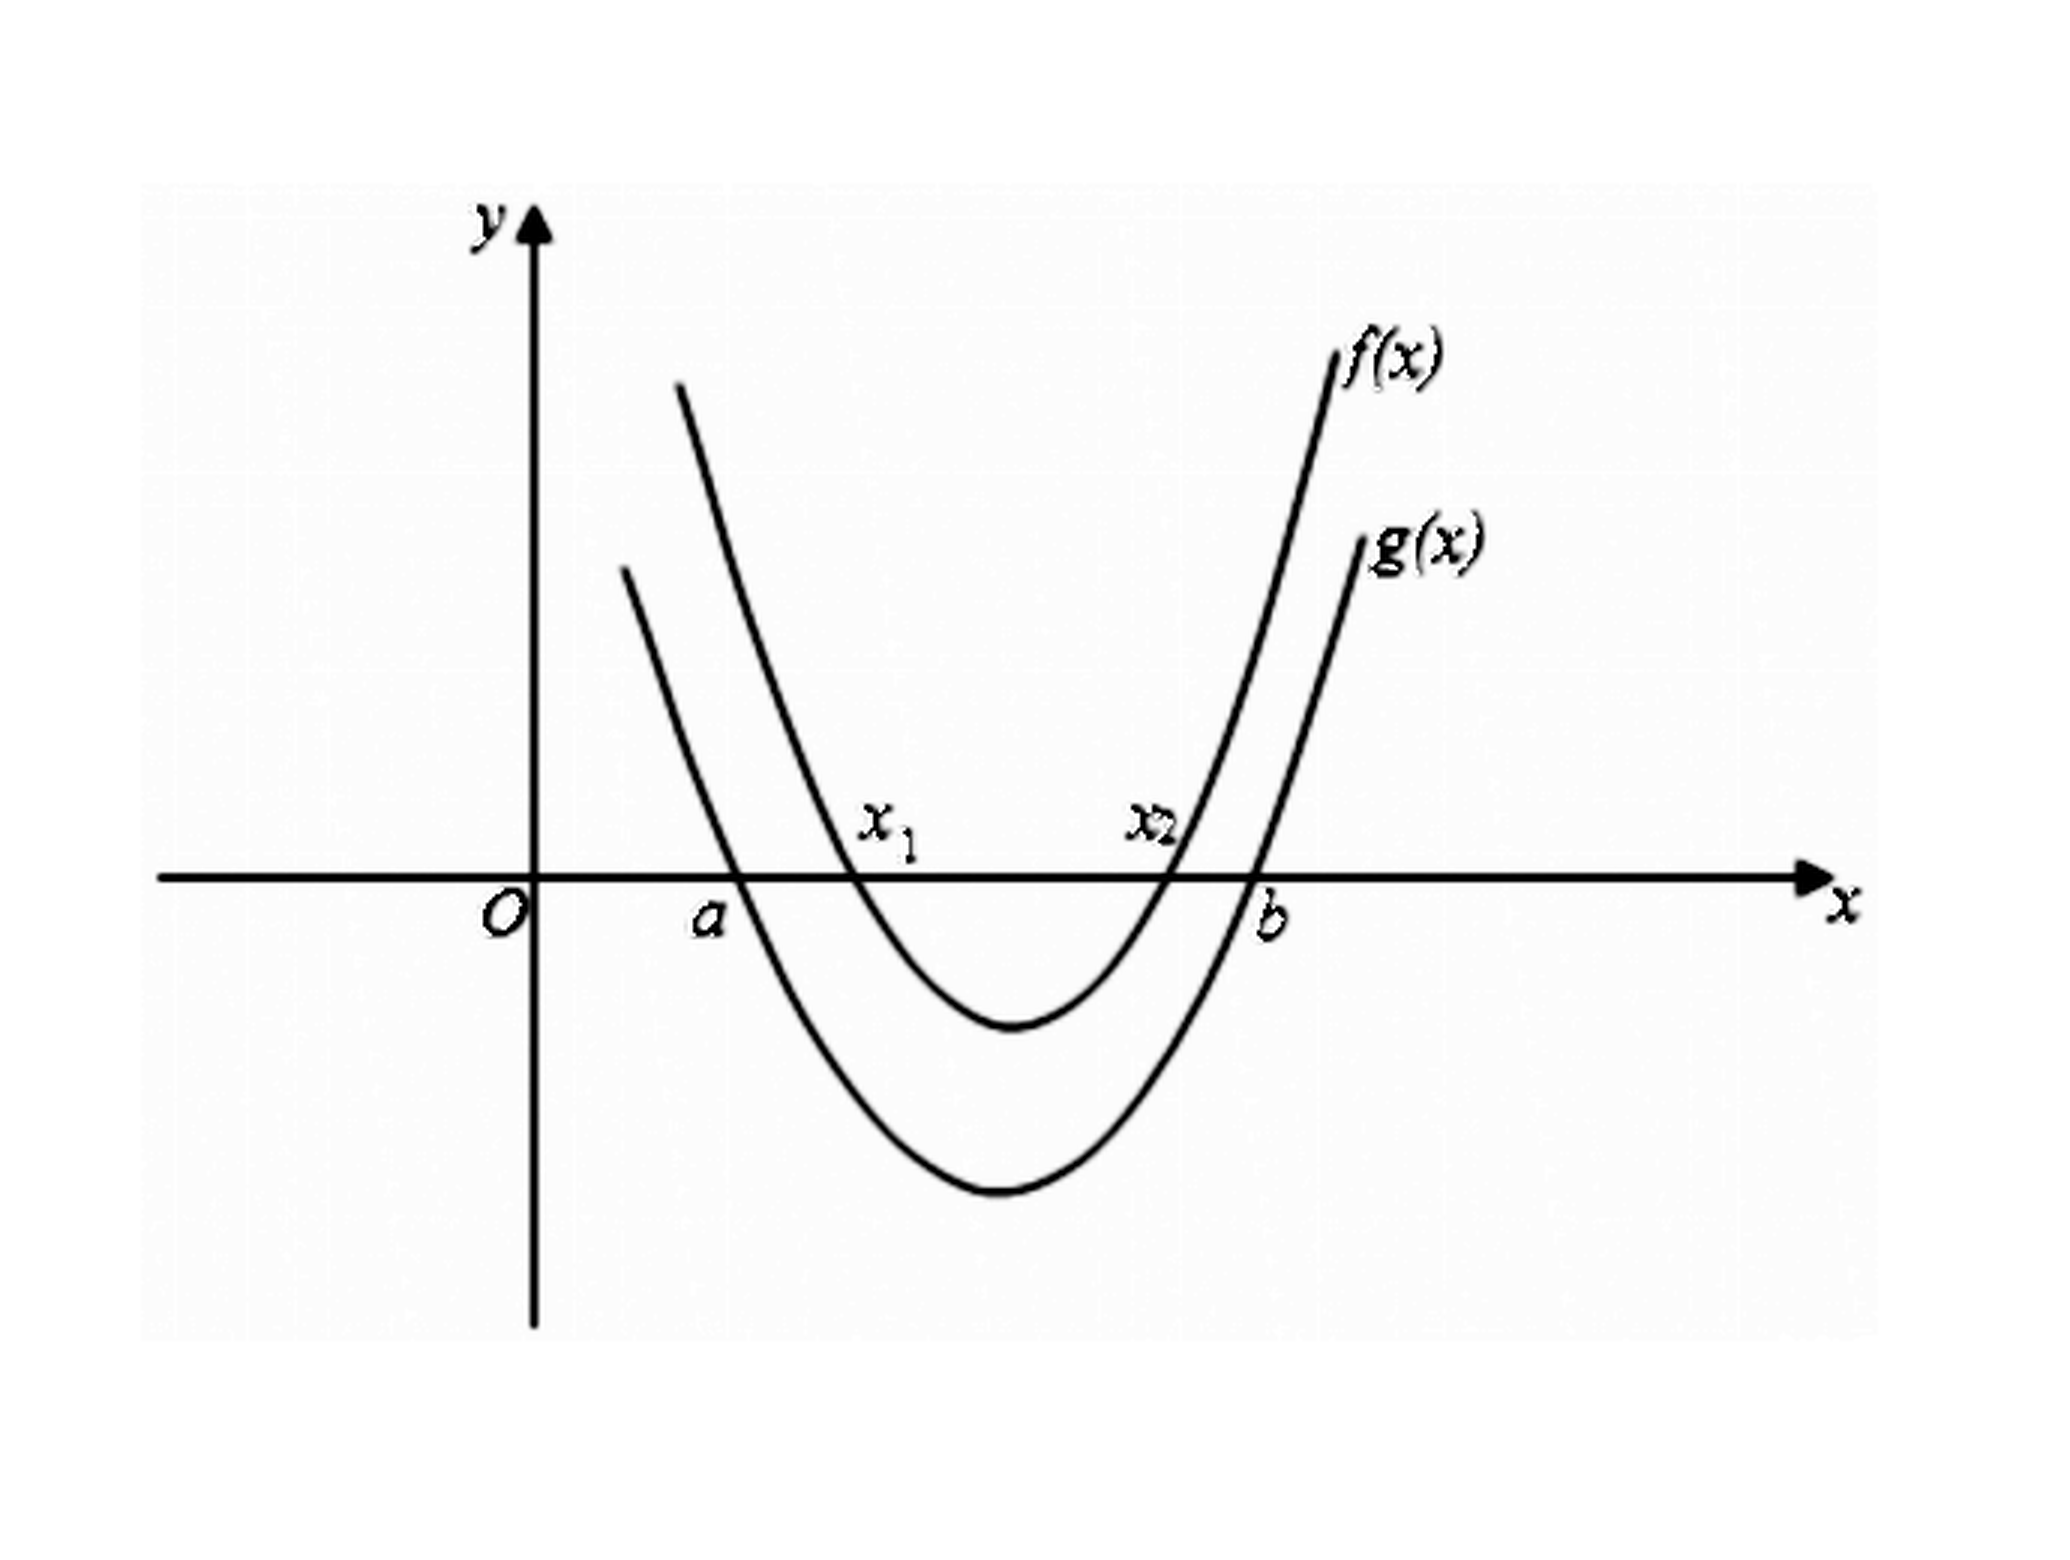
\includegraphics[width=0.52\textwidth]{figures/gao157_q16.png}
\end{center}

\step{由图像得 $a<x_1<x_2<b$，故选 $A$.}
\solend
\fi

\end{enumerate}

\bigsec{三、解答题}

\begin{enumerate}
\setcounter{enumi}{16}

% === Q17 === 解析 6 行；\overline{A}、\varnothing、\subseteq 无、cases
\item 设全集为 $\R$，$m\in\R$，集合 $A=\{x\mid 2<x<5\}$，$B=\{x\mid 2m\leqslant x\leqslant 5m-3\}$.

(1) 若 $m=2$，求 $\overline{A}\cup B$；

(2) 若 $A\cap B=B$，求 $m$ 的取值范围.

\ifanswer
\solbegin
\step{(1) $\overline{A}=\{x\mid x\leqslant2$ 或 $x\geqslant5\}$，当 $m=2$ 时，$B=\{x\mid 4\leqslant x\leqslant7\}$，}
\step{则 $\overline{A}\cup B=\{x\mid x\leqslant2$ 或 $x\geqslant4\}$；}
\step{(2) 因为 $A\cap B=B$，所以 $B$ 是 $A$ 的子集，}
\step{当 $B=\varnothing$ 时，$2m>5m-3$，解得 $m<1$；}
\step{当 $B\ne\varnothing$ 时，$\begin{cases}2m\leqslant5m-3\\2m>2\\5m-3<5\end{cases}$，解得 $1<m<\dfrac85$；}
\step{综上，$m$ 的取值范围是 $(-\infty,1)\cup\left(1,\dfrac85\right)$.}
\solend
\fi

% === Q18 === 解析 2 行；指数式、\lg、换底
\item (1) 设 $a^{2x}=3$，且 $a>0$，求 $\dfrac{a^{3x}+a^{-3x}}{a^x+a^{-x}}$ 的值；

(2) 已知 $\lg2=a, 10^b=3$，用 $a$ 及 $b$ 表示 $\log_{12}25$.

\ifanswer
\solbegin
\step{(1) $\dfrac{a^{3x}+a^{-3x}}{a^x+a^{-x}}=a^{2x}-1+a^{-2x}=3-1+\dfrac13=\dfrac73$；}
\step{(2) $\log_{12}25=\dfrac{\lg25}{\lg12}=\dfrac{2-2\lg2}{2\lg2+\lg3}=\dfrac{2-2a}{2a+b}$.}
\solend
\fi

% === Q19 === 解析 11 行；幂函数、$=0$ 笔误照录、\Delta、\sqrt5、cases
\item 已知幂函数 $f(x)=(m^2+m-1)x^{-2m^2+m+3}$ 在 $(0,+\infty)$ 上为严格增函数.

(1) 求 $f(x)$ 的解析式；

(2) 若 $k+kf(x)>f(x)-x-1$ 对任意实数 $x$ 都成立，求实数 $k$ 的取值范围；

(3) 若关于 $x$ 的不等式 $f(x)\leqslant8x-a$ 的解集中有且仅有 $5$ 个整数，求实数 $a$ 的范围.

\ifanswer
\solbegin
\step{(1) 由题意得 $m^2+m-1=1$，且 $-2m^2+m+3>0$，}
\step{解得 $m=-2$（舍去）或 $m=1$，所以 $f(x)=x^2$；}
\step{(2) $k+kf(x)>f(x)-x-1$ 可化为 $(k-1)x^2+x+k+1=0$ 恒成立，}
\step{当 $k=1$ 时，$x+2>0$，显然不恒成立；}
\step{当 $k\ne1$ 时，要使该二次不等式恒成立，只需 $\begin{cases}k-1>0\\[2pt]\Delta=1-4(k+1)(k-1)\leqslant0\end{cases}$，}
\step{解得 $k\geqslant\dfrac{\sqrt5}{2}$，即所求 $k$ 的范围是 $\left[\dfrac{\sqrt5}{2},+\infty\right)$；}
\step{(3) 不等式 $f(x)\leqslant8x-a$，即 $x^2-8x+a\leqslant0$ 有五个整数解，}
\step{令 $g(x)=x^2-8x+a$，因为该函数开口向上，对称轴为 $x=4$，}
\step{所以解集内的整数为 $2$，$3$，$4$，$5$，$6$，}
\step{由二次函数的性质得，只需 $\begin{cases}g(1)=1-8+a>0\\g(2)=4-8\times2+a\leqslant0\end{cases}$，解得 $7<a\leqslant12$，}
\step{故 $a$ 的取值范围是 $(7,12]$.}
\solend
\fi

% === Q20 === 解析 12 行；材料题、$a+b=1$、大根号、"因出"笔误、分母套分数
\item 问题：正数 $a$、$b$ 满足 $a+b=1$，求 $\dfrac1a+\dfrac2b$ 的最小值.

其中一种解法是：$\dfrac1a+\dfrac2b=\left(\dfrac1a+\dfrac2b\right)(a+b)=1+\dfrac ba+\dfrac{2a}{b}+2\geqslant3+2\sqrt2$，

当且仅当 $\dfrac ba=\dfrac{2a}{b}$ 且 $a+b=1$ 时，即 $a=\sqrt2-1$ 且 $b=2-\sqrt2$ 时取等号.

学习上述解法并解决下列问题：

(1) 若正实数 $x$、$y$ 满足 $x+y=1$，求 $\dfrac2x+\dfrac1y$ 的最小值；

(2) 若实数 $a$、$b$、$x$、$y$ 满足 $\dfrac{x^2}{a^2}-\dfrac{y^2}{b^2}=1$，求证：$a^2-b^2\leqslant(x-y)^2$；

(3) 利用 (2) 的结论，求代数式 $M=\sqrt{2m-5}-\sqrt{m-3}$ 的最小值，并求出使得 $M$ 最小的 $m$ 的值.

\ifanswer
\solbegin
\step{(1) $\dfrac2x+\dfrac1y=(x+y)\left(\dfrac2x+\dfrac1y\right)=3+\dfrac xy+\dfrac{2y}{x}\geqslant3+2\sqrt2$，}
\step{当且仅当 $\dfrac xy=\dfrac{2y}{x}$ 且 $x+y=1$ 时取等号；}
\step{(2) $a^2-b^2=(a^2-b^2)\left(\dfrac{x^2}{a^2}-\dfrac{y^2}{b^2}\right)=x^2+y^2-\left(\dfrac{a^2x^2}{b^2}+\dfrac{b^2y^2}{a^2}\right)$}
\step{$\leqslant x^2+y^2-2\sqrt{\dfrac{a^2x^2}{b^2}\cdot\dfrac{b^2y^2}{a^2}}=x^2+y^2-2xy=(x-y)^2$，}
\step{故当 $b^4x^2=a^4y^2$ 时，等号成立.}
\step{(3) 令 $x=\sqrt{2m-5}, y=\sqrt{m-3}$，由 $\begin{cases}2m-5\geqslant0\\m-3\geqslant0\end{cases}$ 得 $m\geqslant3$，}
\step{$x^2-y^2=(2m-5)-(m-3)=m-2>0$，}
\step{又 $x>0, y>0$，所以 $x>y$，所以 $\dfrac{x^2}{a^2}-\dfrac{y^2}{b^2}=1$，}
\step{由 $x^2-2y^2=1$，得 $\dfrac{x^2}{1}-\dfrac{y^2}{\frac12}=1$，因出 $a^2=1, b^2=\dfrac12$，}
\step{由 (2) 得 $M=\sqrt{2m-5}-\sqrt{m-3}=x-y\geqslant\sqrt{a^2-b^2}=\sqrt{1-\dfrac12}=\dfrac{\sqrt2}{2}$，}
\step{当且仅当 $\dfrac xy=\left(\dfrac ab\right)^2=2$ 取等号，结合 $x^2-2y^2=1$，解得 $x=\sqrt2, y=\dfrac{\sqrt2}{2}$，}
\step{即 $\sqrt{2m-5}=\sqrt2$，得 $m=\dfrac72$，所以 $m=\dfrac72$ 时，$M$ 取得最小值 $\dfrac{\sqrt2}{2}$.}
\solend
\fi

\end{enumerate}

\end{document}
"
% 紧凑版：xelatex "\def\iscompact{1}% 高一157_大境中学_期中.tex
%   —— 高一上数学"2026-2027 年大境中学高一上期中"（试卷版/答案版/紧凑版）
% 试卷版：xelatex 高一157_大境中学_期中.tex
% 答案版：xelatex "\def\isanswer{1}% 高一157_大境中学_期中.tex
%   —— 高一上数学"2026-2027 年大境中学高一上期中"（试卷版/答案版/紧凑版）
% 试卷版：xelatex 高一157_大境中学_期中.tex
% 答案版：xelatex "\def\isanswer{1}\input{高一157_大境中学_期中.tex}"
% 紧凑版：xelatex "\def\iscompact{1}\input{高一157_大境中学_期中.tex}"
%
% ① 原始材料：微信公众号"魔都数学加油站"文章，连载"27学年高一157"，原文标题
% "27学年高一157——2026-2027年上海市大境中学高一上期中"；
% 原文链接：https://mp.weixin.qq.com/s/s6eDMDVkxc2fcBe8LNm-Tw 。
% 正文为 8 张 PNG 页（01/02/03/04/06 为 4762×6735，05/07/08 为 2560×3620，
% 同一篇各页分辨率混排，逐页按各自分辨率裁图核对）。
% 体例：讲评版——填空 3—12（10 题）、选择 13—16（4 题）、解答 17—20（4 题），
% 共 18 题，自第 3 题起编（1、2 未印在本篇）；末题是第 20 题（不是 21）。
% 除第 4 题只印【答案】外，其余 17 题逐题印【解析】（逐题核实，见 ②）。
% 题目、答案、解析均据原图转录；卷面粉红色水印"魔都数学加油站"及公众号
% 页脚未录入。
% 全卷仅 1 幅配图：第 16 题解析内函数图像（"设 g(x)=(x-a)(x-b)，
% f(x)=g(x)+1，画出函数 g(x) 与函数 f(x) 的图像，如图所示"），
% 解析内配图仅答案版出，裁 figures/gao157_q16.png；逐页通读 8 页确认
% 无题目配图、无表格；08 页下半仅水印、无正文。
%
% 卷首标题：原卷印作"2026-2027 年大境中学高一上期中"，年份区间按全稿惯例排 en dash；
% 原卷卷面未印副标题，本稿按同期中卷知识模块口径补出"集合与常用逻辑用语、不等式、函数"。
%
% ② 与原卷的排版差异：
%   ① 原文从第 3 题起，本稿保留原题号；共 18 题三节，解答题 4 题到 20；
%      三节各自 \begin{enumerate}…\end{enumerate} + \setcounter{enumi}{2/12/16}
%      （题目溯源.py 按 \bigsec 切节、每节独立计 depth，只收 depth==1 的 \item，
%       见 高一156 头注②的订正）；
%   ② 第 4 题只印【答案】、无【解析】，提 \ans{}；其余 17 题逐题印【解析】、
%      逐题设 \solbegin…\solend；四道选择题答案在解析末句"故选 D／D／C／A"
%      （逐个放大复核）、括号 \mbox{（\quad）} 留空；答案版【答案】/【解析】
%      标记数 = 18 = 全卷题数（1 个 \ans ＋ 17 个 \solbegin）；
%   ③ 原卷卷面未印副标题，本稿按知识模块口径补出；
%   ④ 原卷填空横线按全稿惯例排 \blankline[4.4em]；选择题选项段前按惯例各加
%      \keepwithprev；解答题不留作答区、不加 \anspace（原卷为讲评版，109—113 起
%      全稿不用 \anspace）；
%   ⑤ 数集：Q4"$x、y\in R$"、Q6"$x\in R$"、Q10"$a\in Z$"、Q12"$n\in Z$"
%      "$n_1、n_2\in Z$"、Q17"全集为 R／$m\in R$"原卷印斜体 R/Z，按全稿惯例
%      归一 \R／\Z（参见 高一14 头注④、高一150 头注②⑤、高一153 头注⑤）；
%      绝对值排 \lvert…\rvert（Q6 $\lvert x-1\rvert$／$\lvert x+3\rvert$／
%      $\lvert 2x+2\rvert$），集合描述竖线排 \mid（Q12、Q17），空集 \varnothing
%      （Q17"$B=\varnothing$"），补集照原卷上划线排 \overline{A}（Q17），
%      不等号按全稿惯例排 \leqslant／\geqslant；
%   ⑥ 判别式三处（Q8"$\Delta=(-2m)^2-4(m+2)$"、Q15"$\Delta=(a+2)^2+4(a^2-4)<0$"、
%      Q19"$\Delta=1-4(k+1)(k-1)\leqslant0$"）放大比对同形、均为等腰偏高且右斜边
%      加粗的 \Delta，统一照录 \Delta；本卷无扁三角 \triangle 用例（与 高一142／
%      高一151／高一152 的 Δ/△ 混用卷不同）；
%   ⑦ "图像／图象"逐处照录不统一：Q9"图像过点 $(4,2)$""它的图像过点"、
%      Q16"画出函数 $g(x)$ 与函数 $f(x)$ 的图像""由图像得"用"图像"；
%      Q14 题干及解析四处均用"图象"（"的图象关于原点对称""图象关于 $y$ 轴对称"）；
%   ⑧ 原卷笔误／未化简式照录：
%      · Q5 解析"$2\sqrt4+1=5$"根号 4 原卷未化简，照录 \sqrt4；
%      · Q7 解析"$\lg\frac{E_1}{E_2}=\frac25\cdot(m_2-m_1)=\frac25(-1.45+26.7)=10.1$"
%        第一处有 \cdot、第二处无，逐处照录；题干"$m_1-m_2=-\frac52\lg\frac{E_1}{E_2}$"；
%      · Q10 解析"$f(1)=\frac{a+1}{1+2}\geqslant0$"与 cases 第二行分母均印 $1+2$、
%        未化简成 $3$，照录；
%      · Q19 (2)"可化为 $(k-1)x^2+x+k+1=0$ 恒成立"原卷印 $=0$（与 >0 恒成立
%        的题意不符），照录笔误；
%      · Q20 (3)"因出 $a^2=1, b^2=\frac12$"原卷印"因出"（当作"因此"），照录；
%      · Q20 (3)"得 $\frac{x^2}{1}-\frac{y^2}{\frac12}=1$"分母套分数、照录；
%   ⑨ 圈数字①②在文本模式（Q15 解析"①当 $a^2-4=0$ 时""②当 $a^2-4\ne0$ 时"，
%      共 2 枚）；子题标号 (1)(2)(3) 半角括号照录；行末西文句点 ASCII `.`；
%      行中全角逗号／顿号照录；半角逗号在数学组之间是全稿惯例、非笔误
%      （Q8"$x_1+x_2=2m, x_1x_2=m+2$"、Q12"$n\in Z$"、Q18"$\lg2=a, 10^b=3$"、
%      Q20"$a^2=1, b^2=\frac12$"等）；中文弯引号""照录（Q4 命题）；
%   ⑩ 自定义名词：Q11"交叉数"、Q12"$a\otimes b$"新定义运算、Q20"问题／
%      其中一种解法是／学习上述解法并解决下列问题"材料题，均照原卷录入；
%   ⑪ 配图：全卷 1 幅（逐页通读 8 页确认）——Q16 解析内函数图像（05 页右侧，
%      $f(x)$ 与 $g(x)$ 两条抛物线、标注 $a,x_1,x_2,b$），仅答案版出，
%      裁 figures/gao157_q16.png，去粉色水印、去色、3× LANCZOS 放大；
%      图放 \ifanswer 内 \solbegin…\solend 的两 \step 之间（高一108 第 6 题／
%      高一156 Q15 成例）；Q16 题干无"如图"、不需题目配图守卫。
%
% ③ 行数复核：一条 \step = 原卷解析的一个印刷行，cases 块作一个印刷行计；
%    跨半页重叠行（Q5 的"【解析】x-1>0…"、Q10 的"所以 a=-1 或 a=0"、
%    Q12 的"【解析】由 u⊗v…"、Q14 的"f(x)=x² 图象关于 y 轴对称"、
%    Q19 的"(1) 由题意得…"、Q20 的"(3) 令 x=…"等 hi_1/hi_2 两半页共有的行）
%    只计一次，别把原卷折行并起来。
%    逐题数（主会话逐页核对定稿）：Q3：1；Q4：0（只印【答案】、提 \ans{}，
%    不计入 \step 账）；Q5：2；Q6：5；Q7：2；Q8：5；Q9：3；Q10：4；
%    Q11：3；Q12：6；Q13：3；Q14：5；Q15：9；Q16：4；Q17：6；Q18：2；
%    Q19：11；Q20：12。合计 83 条 \step（本卷无 \stepm），与原卷逐题印刷行相等。
%    全卷 18 题：1 题只印【答案】（\ans）、17 题印【解析】（\solbegin…\solend），
%    答案版【答案】/【解析】标记数 = 18 = 全卷题数。
%    全卷除此 6 类外未发现其它笔误／自相矛盾处；17 题印【解析】、1 题印【答案】。
%
\documentclass[a4paper,11pt]{article}
\usepackage{common}

\begin{document}

\examtitlest[3]{2026--2027 年大境中学高一上期中}{集合与常用逻辑用语、不等式、函数}

\bigsec{一、填空题}

\begin{enumerate}
\setcounter{enumi}{2}

% === Q3 === 解析 1 行；$a,b$ 半角逗号照录
\item 若 $a=x^2-2x+1$，$b=x-3$，则 $a,b$ 的大小关系为\blankline[4.4em].

\ifanswer
\solbegin
\step{$a-b=x^2-3x+4=\left(x-\dfrac32\right)^2+\dfrac74>0$，所以 $a>b$.}
\solend
\fi

% === Q4 === 只印【答案】、无【解析】；中文弯引号、\R、顿号；提 \ans{}
\item 用反证法证明命题：“设 $x$、$y\in\R$. 若 $x+y>2$，则 $x>1$ 或 $y>1$”时，假设的内容应该是\blankline[4.4em].

\ifanswer
\ans{$x\leqslant1$ 且 $y\leqslant1$}
\fi

% === Q5 === 解析 2 行；$2\sqrt4+1=5$ 根号 4 未化简照录
\item 当 $x>1$ 时，$x+\dfrac4{x-1}$ 的最小值为\blankline[4.4em].

\ifanswer
\solbegin
\step{$x-1>0$，$x+\dfrac4{x-1}=(x-1)+\dfrac4{x-1}+1\geqslant2\sqrt4+1=5$，}
\step{当且仅当 $x-1=\dfrac4{x-1}$，即 $x=3$ 时取等号，故最小值为 $5$.}
\solend
\fi

% === Q6 === 解析 5 行；绝对值 \lvert…\rvert、\cup、\R
\item 设 $x\in\R$，方程 $\lvert x-1\rvert+\lvert x+3\rvert=\lvert 2x+2\rvert$ 的解集是\blankline[4.4em].

\ifanswer
\solbegin
\step{当 $x\leqslant-3$ 时，方程为 $1-x-x-3=-2x-2$，等式成立；}
\step{当 $-3<x\leqslant-1$ 时，方程为 $1-x+x+3=-2x-2$，解得 $x=-3$，舍去；}
\step{当 $-1<x<1$ 时，方程为 $1-x+x+3=2x+2$，解得 $x=1$，舍去；}
\step{当 $x\geqslant1$ 时，方程为 $x-1+x+3=2x+2$，等式成立，}
\step{综上，方程 $\lvert x-1\rvert+\lvert x+3\rvert=\lvert 2x+2\rvert$ 的解集为 $(-\infty,-3]\cup[1,+\infty)$.}
\solend
\fi

% === Q7 === 解析 2 行；星等材料题、\lg、\cdot 逐处照录、天狼星
\item 在天文学中，天体的明暗程度可以用星等或亮度来描述，两颗星的星等与亮度满足 $m_1-m_2=-\dfrac52\lg\dfrac{E_1}{E_2}$，其中星等为 $m_k$ 的星的亮度为 $E_k(k=1,2)$. 已知太阳的星等为 $-26.7$，天狼星的星等为 $-1.45$，则太阳与天狼星的亮度的比值为\blankline[4.4em].

\ifanswer
\solbegin
\step{两颗星的星等与亮度满足 $m_1-m_2=-\dfrac52\lg\dfrac{E_1}{E_2}$，令 $m_2=-1.45$，$m_1=-26.7$，}
\step{$\lg\dfrac{E_1}{E_2}=\dfrac25\cdot(m_2-m_1)=\dfrac25(-1.45+26.7)=10.1$，$\dfrac{E_1}{E_2}=10^{10.1}$.}
\solend
\fi

% === Q8 === 解析 5 行；韦达定理、判别式 \Delta、半角逗号在数学组间
\item 已知方程 $x^2-2mx+m+2=0$ 有两个实数根 $x_1,x_2$，满足 $x_1^2+x_2^2=2$，则实数 $m$ 的值为\blankline[4.4em].

\ifanswer
\solbegin
\step{对于方程 $x^2-2mx+m+2=0$，由韦达定理得 $x_1+x_2=2m, x_1x_2=m+2$，}
\step{又 $x_1^2+x_2^2=(x_1+x_2)^2-2x_1x_2=(2m)^2-2(m+2)=4m^2-2m-4=2$，}
\step{解得 $m=\dfrac32$ 或 $m=-1$，}
\step{因为方程有两个实数根，所以 $\Delta=(-2m)^2-4(m+2)=4m^2-4m-8\geqslant0$，}
\step{解得 $m\leqslant-1$ 或 $m\geqslant2$，故 $m=-1$.}
\solend
\fi

% === Q9 === 解析 3 行；"图像"照录、$x^\alpha$、$x^{1/2}=\sqrt{x}$
\item 已知幂函数 $y=f(x)$ 的图像过点 $(4,2)$，则不等式 $f(x^2-2x)<f(2-x)$ 的解集为\blankline[4.4em].

\ifanswer
\solbegin
\step{设幂函数 $y=f(x)=x^\alpha$，它的图像过点 $(4,2)$，所以 $4^\alpha=2$，$\alpha=\dfrac12$，}
\step{故 $f(x)=x^{\frac12}=\sqrt{x}$，由不等式 $f(x^2-2x)<f(2-x)$，}
\step{得 $0\leqslant x^2-2x<2-x$，得 $-1<x\leqslant0$，故解集为 $(-1,0]$.}
\solend
\fi

% === Q10 === 解析 4 行；$a\in\Z$、cases（分母 $1+2$ 未化简）、参数分离
\item 已知函数 $y=\dfrac{ax+1}{x+2}$（常数 $a\in\Z$）. 要使该函数在区间 $[1,+\infty)$ 上是严格减函数，并且函数值不恒为负，则满足条件的 $a$ 的取值为\blankline[4.4em].

\ifanswer
\solbegin
\step{函数参数分离为 $y=\dfrac{a(x+2)+1-2a}{x+2}=a+\dfrac{1-2a}{x+2}$，}
\step{若函数在区间 $[1,+\infty)$ 上严格减函数，则 $1-2a>0$，}
\step{且函数的最大值 $f(1)=\dfrac{a+1}{1+2}\geqslant0$，即 $\begin{cases}1-2a>0\\[2pt]\dfrac{a+1}{1+2}\geqslant0\end{cases}$，解得 $-1\leqslant a<\dfrac12$，又 $a\in\Z$，}
\step{所以 $a=-1$ 或 $a=0$.}
\solend
\fi

% === Q11 === 解析 3 行；"交叉数"自定义名词、$(-1)^t$、$2^5$、$32\times3=96$
\item 对非空集合 $A$ 中的每个元素 $t$，都乘以 $(-1)^t$ 再求和，称为集合 $A$ 的交叉数，例如 $A=\{2,3,6\}$，则集合 $A$ 的交叉数为 $(-1)^2\cdot2+(-1)^3\cdot3+(-1)^6\cdot6=5$. 若集合 $W=\{1,2,3,4,5,6\}$，则 $W$ 的所有非空子集的交叉数的总和为\blankline[4.4em].

\ifanswer
\solbegin
\step{固定 $W$ 中的任一元素，其余 $5$ 个元素各有选或不选两种情况，}
\step{因此该元素出现在 $2^5$ 个非空子集中，}
\step{所有交叉数的总和为 $2^5(-1+2-3+4-5+6)=32\times3=96$.}
\solend
\fi

% === Q12 === 解析 6 行；\otimes、\lambda、\mid、\Z、\times 与 \cdot 逐处照录
\item 对于任意两个正实数 $a$、$b$，定义 $a\otimes b=\lambda\cdot\dfrac ab$，其中常数 $\lambda\in\left(\dfrac{\sqrt2}{2},1\right)$. 若 $u\geqslant v>0$，且 $u\otimes v$ 与 $v\otimes u$ 都是集合 $\left\{x\mid x=\dfrac n2,n\in\Z\right\}$ 的元素，则 $u\otimes v=$\blankline[4.4em].

\ifanswer
\solbegin
\step{由 $u\otimes v$ 与 $v\otimes u$ 都是集合 $\left\{x\mid x=\dfrac n2,n\in\Z\right\}$ 的元素，}
\step{不妨设 $\lambda\times\dfrac uv=\dfrac12 n_1$，$\lambda\times\dfrac vu=\dfrac12 n_2$，$n_1$、$n_2\in\Z$，}
\step{因为 $u\geqslant v>0$，所以 $0<\dfrac vu\leqslant1$，因为 $\lambda\in\left(\dfrac{\sqrt2}{2},1\right)$，所以 $\dfrac12 n_2=\lambda\cdot\dfrac vu\in(0,1)$，}
\step{因为 $n_2\in\Z$，所以 $n_2=1$，即 $\dfrac12=\dfrac{\lambda v}{u}$，所以 $\lambda=\dfrac{u}{2v}\in\left(\dfrac{\sqrt2}{2},1\right)$，}
\step{所以 $\dfrac uv\in(\sqrt2,2)$，$\dfrac{u^2}{v^2}\in(2,4)$，则 $\lambda\cdot\dfrac uv=\dfrac{u^2}{v^2}\times\dfrac12=\dfrac12 n_1\in(1,2)$，}
\step{因为 $n_1\in\Z$，所以 $n_1=3$，$\dfrac12 n_1=\dfrac32$，故 $u\otimes v=\dfrac32$.}
\solend
\fi

\end{enumerate}

\bigsec{二、选择题}

\begin{enumerate}
\setcounter{enumi}{12}

% === Q13 === 解析 3 行；选项段 \keepwithprev；故选 D
\item 下列不等式成立的为\mbox{（\quad）}

\keepwithprev
A. 若 $a>b$，则 $ac^2>bc^2$\qquad B. 若 $a>b$，则 $a^2>b^2$

C. 若 $a>b$，$c>d$，则 $a+b>c+d$\qquad D. 若 $a>b$，则 $a^3>b^3$

\ifanswer
\solbegin
\step{A 中 $c=0$ 时不成立；B 取 $a=1$，$b=-2$ 不成立；}
\step{C 取 $a=1$，$b=0$，$c=5$，$d=0$ 不成立.}
\step{幂函数 $y=x^3$ 在实数集上严格递增，所以 $a>b\Rightarrow a^3>b^3$，故选 $D$.}
\solend
\fi

% === Q14 === 解析 5 行；"图象"四处照录；故选 D
\item 幂函数 $f(x)=x^\alpha$ 的图象关于原点对称，且在 $(-\infty,0)$ 上是严格增函数，则 $f(x)$ 可以是\mbox{（\quad）}

\keepwithprev
A. $f(x)=x^{-1}$\qquad B. $f(x)=x^{\frac12}$\qquad C. $f(x)=x^2$\qquad D. $f(x)=x^3$

\ifanswer
\solbegin
\step{$f(x)=\dfrac1x$ 的图象关于原点对称，在 $(-\infty,0)$ 上是严格减函数，故 $A$ 错误；}
\step{$f(x)=x^{\frac12}$ 在 $(-\infty,0)$ 上无意义，故 $B$ 错误；}
\step{$f(x)=x^2$ 图象关于 $y$ 轴对称，故 $C$ 错误；}
\step{$f(x)=x^3$ 的图象关于原点对称，且在 $(-\infty,0)$ 上是严格增函数，故 $D$ 正确.}
\step{故选 $D$.}
\solend
\fi

% === Q15 === 解析 9 行；圈数字①②、\Delta、cases；故选 C
\item 若关于 $x$ 的不等式 $(a^2-4)x^2+(a+2)x-1\geqslant0$ 的解集不为空集，则实数 $a$ 的取值范围为\mbox{（\quad）}

\keepwithprev
A. $\left(-2,\dfrac65\right]$\qquad B. $\left[-2,\dfrac65\right]$

C. $(-\infty,-2)\cup\left[\dfrac65,+\infty\right)$\qquad D. $(-\infty,-2]\cup\left[\dfrac65,+\infty\right)$

\ifanswer
\solbegin
\step{①当 $a^2-4=0$ 时，$a=\pm2$，}
\step{若 $a=2$ 时，原不等式为 $4x-1\geqslant0$，则不等式的解集不是空集；}
\step{若 $a=-2$ 时，原不等式为 $-1\geqslant0$，无解，不符合题意；}
\step{②当 $a^2-4\ne0$ 时，$a\ne\pm2$，}
\step{若 $(a^2-4)x^2+(a+2)x-1\geqslant0$ 的解集是空集，则 $\begin{cases}a^2-4<0\\[2pt]\Delta=(a+2)^2+4(a^2-4)<0\end{cases}$，}
\step{解得 $-2<a<\dfrac65$，}
\step{则当不等式 $(a^2-4)x^2+(a+2)x-1\geqslant0$ 的解集不为空集时，}
\step{有 $a<-2$ 或 $a\geqslant\dfrac65$ 且 $a\ne2$，}
\step{综上，实数 $a$ 的取值范围为 $(-\infty,-2)\cup\left[\dfrac65,+\infty\right)$，故选 $C$.}
\solend
\fi

% === Q16 === 解析 4 行＋1 幅解析内配图（仅答案版）；"图像"照录；故选 A
\item 已知实数 $a<b$，关于 $x$ 的不等式 $x^2-(a+b)x+ab+1<0$ 的解集为 $(x_1,x_2)$，则实数 $a$、$b$、$x_1$、$x_2$ 从小到大的排列是\mbox{（\quad）}

\keepwithprev
A. $a<x_1<x_2<b$\qquad B. $x_1<a<b<x_2$\qquad C. $a<x_1<b<x_2$\qquad D. $x_1<a<x_2<b$

\ifanswer
\solbegin
\step{不等式 $x^2-(a+b)x+ab+1<0$ 可化为 $(x-a)(x-b)+1<0$，}
\step{设 $g(x)=(x-a)(x-b)$，$f(x)=g(x)+1$，}
\step{画出函数 $g(x)$ 与函数 $f(x)$ 的图像，如图所示，}

\begin{center}
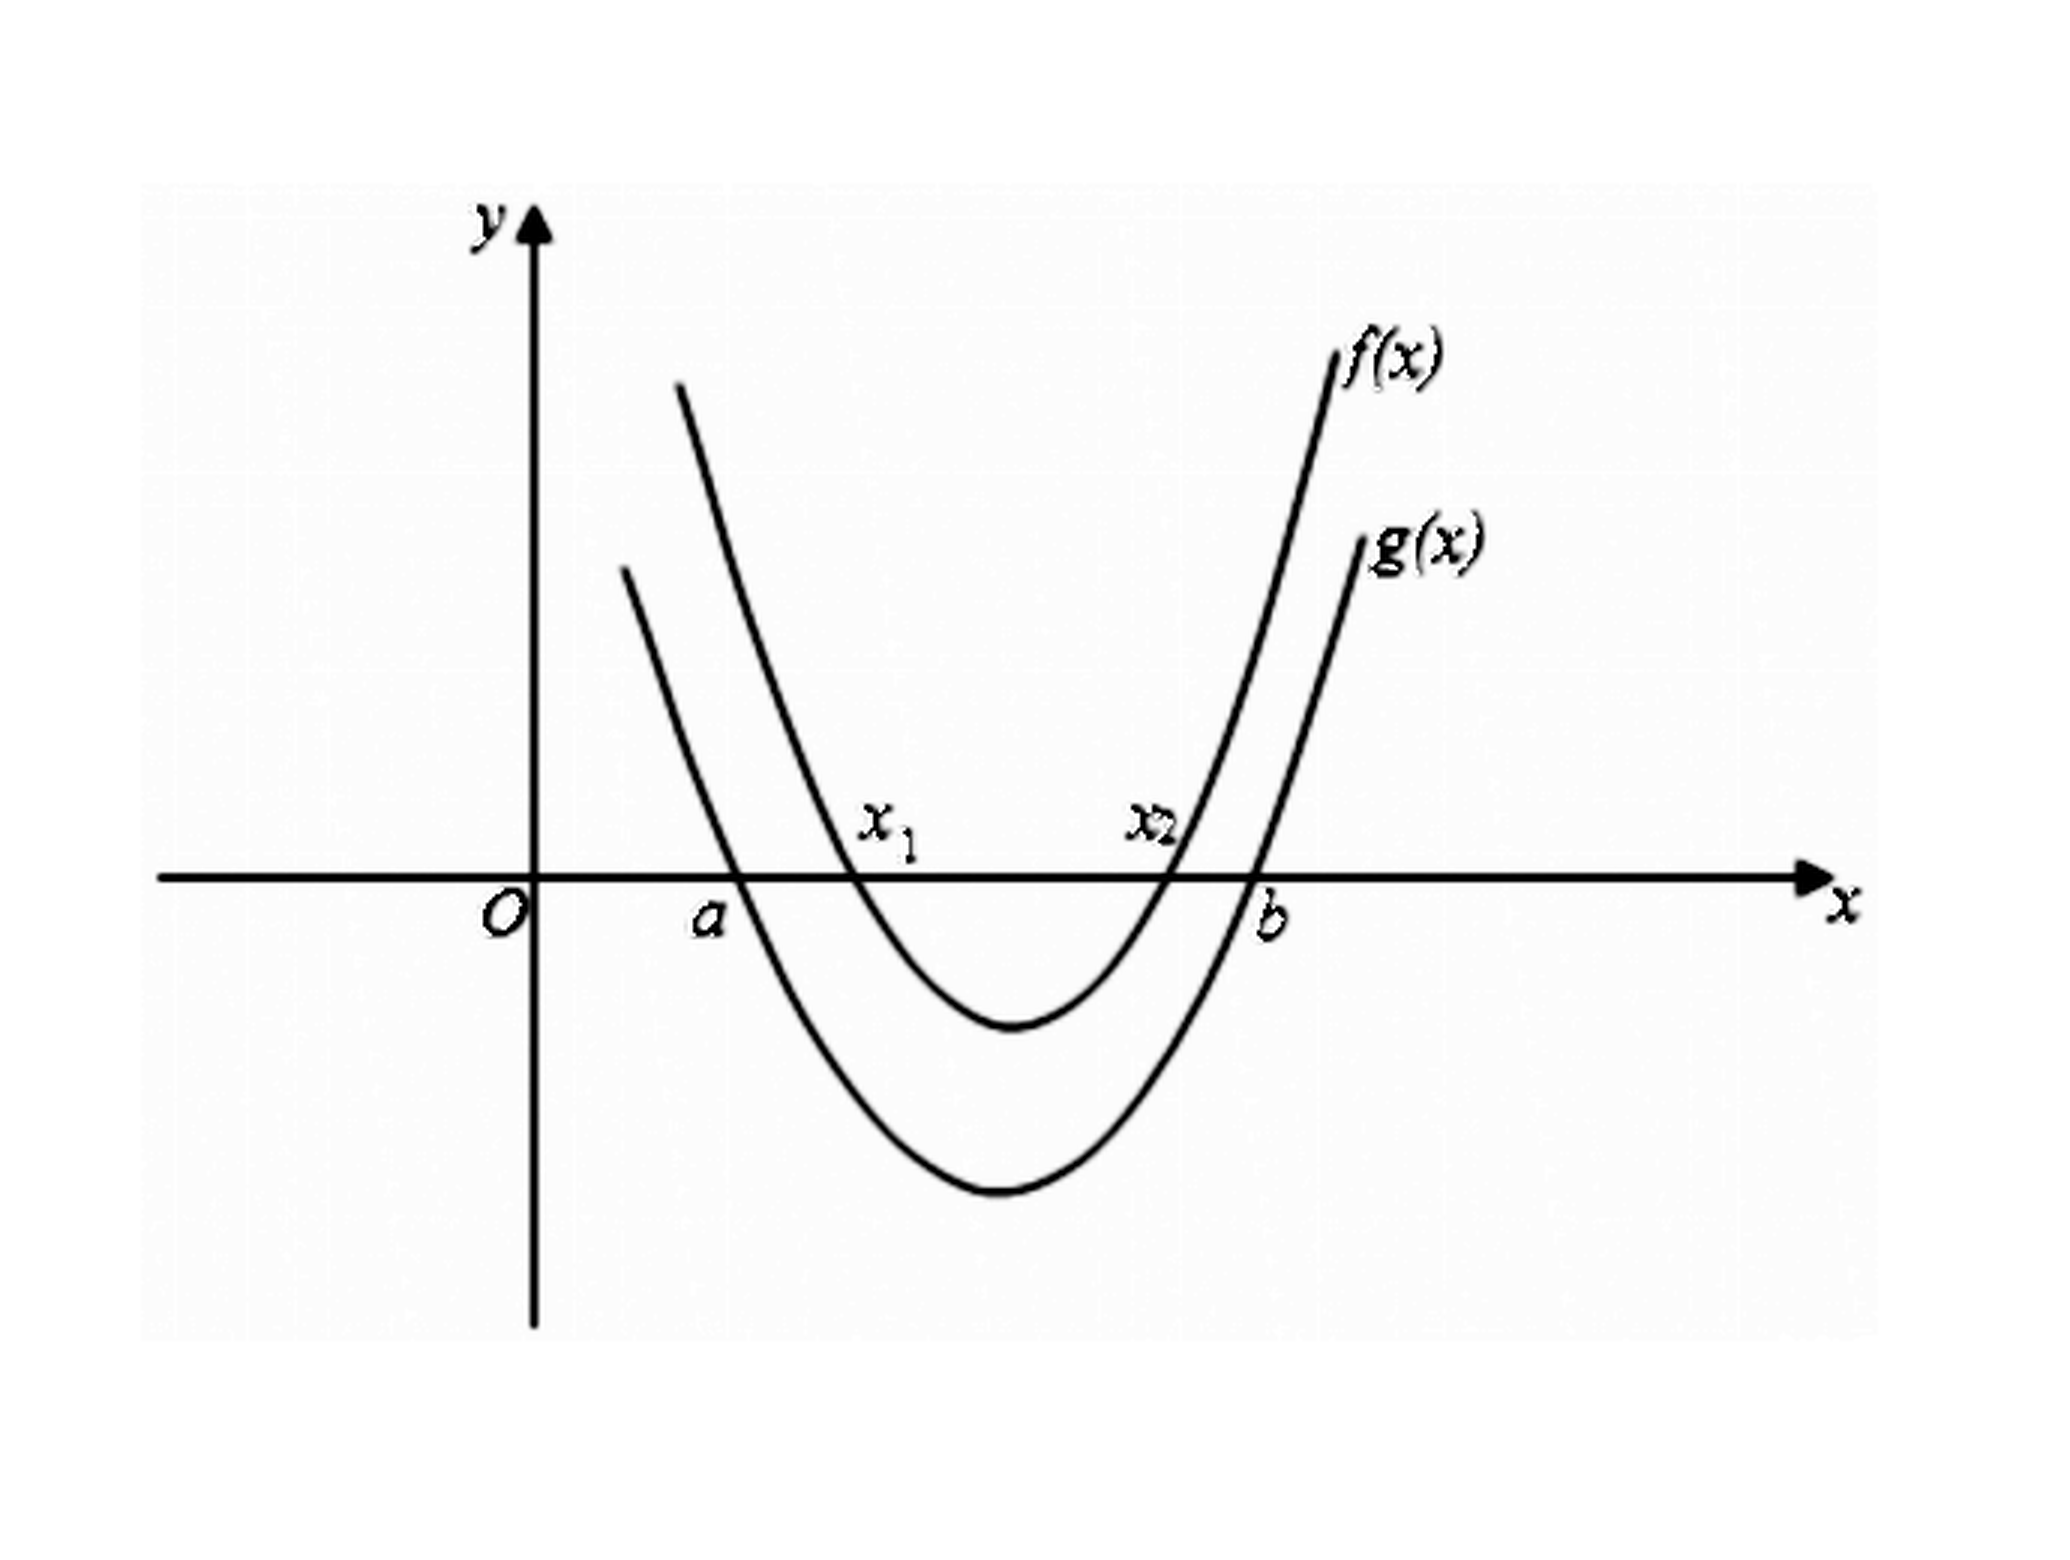
\includegraphics[width=0.52\textwidth]{figures/gao157_q16.png}
\end{center}

\step{由图像得 $a<x_1<x_2<b$，故选 $A$.}
\solend
\fi

\end{enumerate}

\bigsec{三、解答题}

\begin{enumerate}
\setcounter{enumi}{16}

% === Q17 === 解析 6 行；\overline{A}、\varnothing、\subseteq 无、cases
\item 设全集为 $\R$，$m\in\R$，集合 $A=\{x\mid 2<x<5\}$，$B=\{x\mid 2m\leqslant x\leqslant 5m-3\}$.

(1) 若 $m=2$，求 $\overline{A}\cup B$；

(2) 若 $A\cap B=B$，求 $m$ 的取值范围.

\ifanswer
\solbegin
\step{(1) $\overline{A}=\{x\mid x\leqslant2$ 或 $x\geqslant5\}$，当 $m=2$ 时，$B=\{x\mid 4\leqslant x\leqslant7\}$，}
\step{则 $\overline{A}\cup B=\{x\mid x\leqslant2$ 或 $x\geqslant4\}$；}
\step{(2) 因为 $A\cap B=B$，所以 $B$ 是 $A$ 的子集，}
\step{当 $B=\varnothing$ 时，$2m>5m-3$，解得 $m<1$；}
\step{当 $B\ne\varnothing$ 时，$\begin{cases}2m\leqslant5m-3\\2m>2\\5m-3<5\end{cases}$，解得 $1<m<\dfrac85$；}
\step{综上，$m$ 的取值范围是 $(-\infty,1)\cup\left(1,\dfrac85\right)$.}
\solend
\fi

% === Q18 === 解析 2 行；指数式、\lg、换底
\item (1) 设 $a^{2x}=3$，且 $a>0$，求 $\dfrac{a^{3x}+a^{-3x}}{a^x+a^{-x}}$ 的值；

(2) 已知 $\lg2=a, 10^b=3$，用 $a$ 及 $b$ 表示 $\log_{12}25$.

\ifanswer
\solbegin
\step{(1) $\dfrac{a^{3x}+a^{-3x}}{a^x+a^{-x}}=a^{2x}-1+a^{-2x}=3-1+\dfrac13=\dfrac73$；}
\step{(2) $\log_{12}25=\dfrac{\lg25}{\lg12}=\dfrac{2-2\lg2}{2\lg2+\lg3}=\dfrac{2-2a}{2a+b}$.}
\solend
\fi

% === Q19 === 解析 11 行；幂函数、$=0$ 笔误照录、\Delta、\sqrt5、cases
\item 已知幂函数 $f(x)=(m^2+m-1)x^{-2m^2+m+3}$ 在 $(0,+\infty)$ 上为严格增函数.

(1) 求 $f(x)$ 的解析式；

(2) 若 $k+kf(x)>f(x)-x-1$ 对任意实数 $x$ 都成立，求实数 $k$ 的取值范围；

(3) 若关于 $x$ 的不等式 $f(x)\leqslant8x-a$ 的解集中有且仅有 $5$ 个整数，求实数 $a$ 的范围.

\ifanswer
\solbegin
\step{(1) 由题意得 $m^2+m-1=1$，且 $-2m^2+m+3>0$，}
\step{解得 $m=-2$（舍去）或 $m=1$，所以 $f(x)=x^2$；}
\step{(2) $k+kf(x)>f(x)-x-1$ 可化为 $(k-1)x^2+x+k+1=0$ 恒成立，}
\step{当 $k=1$ 时，$x+2>0$，显然不恒成立；}
\step{当 $k\ne1$ 时，要使该二次不等式恒成立，只需 $\begin{cases}k-1>0\\[2pt]\Delta=1-4(k+1)(k-1)\leqslant0\end{cases}$，}
\step{解得 $k\geqslant\dfrac{\sqrt5}{2}$，即所求 $k$ 的范围是 $\left[\dfrac{\sqrt5}{2},+\infty\right)$；}
\step{(3) 不等式 $f(x)\leqslant8x-a$，即 $x^2-8x+a\leqslant0$ 有五个整数解，}
\step{令 $g(x)=x^2-8x+a$，因为该函数开口向上，对称轴为 $x=4$，}
\step{所以解集内的整数为 $2$，$3$，$4$，$5$，$6$，}
\step{由二次函数的性质得，只需 $\begin{cases}g(1)=1-8+a>0\\g(2)=4-8\times2+a\leqslant0\end{cases}$，解得 $7<a\leqslant12$，}
\step{故 $a$ 的取值范围是 $(7,12]$.}
\solend
\fi

% === Q20 === 解析 12 行；材料题、$a+b=1$、大根号、"因出"笔误、分母套分数
\item 问题：正数 $a$、$b$ 满足 $a+b=1$，求 $\dfrac1a+\dfrac2b$ 的最小值.

其中一种解法是：$\dfrac1a+\dfrac2b=\left(\dfrac1a+\dfrac2b\right)(a+b)=1+\dfrac ba+\dfrac{2a}{b}+2\geqslant3+2\sqrt2$，

当且仅当 $\dfrac ba=\dfrac{2a}{b}$ 且 $a+b=1$ 时，即 $a=\sqrt2-1$ 且 $b=2-\sqrt2$ 时取等号.

学习上述解法并解决下列问题：

(1) 若正实数 $x$、$y$ 满足 $x+y=1$，求 $\dfrac2x+\dfrac1y$ 的最小值；

(2) 若实数 $a$、$b$、$x$、$y$ 满足 $\dfrac{x^2}{a^2}-\dfrac{y^2}{b^2}=1$，求证：$a^2-b^2\leqslant(x-y)^2$；

(3) 利用 (2) 的结论，求代数式 $M=\sqrt{2m-5}-\sqrt{m-3}$ 的最小值，并求出使得 $M$ 最小的 $m$ 的值.

\ifanswer
\solbegin
\step{(1) $\dfrac2x+\dfrac1y=(x+y)\left(\dfrac2x+\dfrac1y\right)=3+\dfrac xy+\dfrac{2y}{x}\geqslant3+2\sqrt2$，}
\step{当且仅当 $\dfrac xy=\dfrac{2y}{x}$ 且 $x+y=1$ 时取等号；}
\step{(2) $a^2-b^2=(a^2-b^2)\left(\dfrac{x^2}{a^2}-\dfrac{y^2}{b^2}\right)=x^2+y^2-\left(\dfrac{a^2x^2}{b^2}+\dfrac{b^2y^2}{a^2}\right)$}
\step{$\leqslant x^2+y^2-2\sqrt{\dfrac{a^2x^2}{b^2}\cdot\dfrac{b^2y^2}{a^2}}=x^2+y^2-2xy=(x-y)^2$，}
\step{故当 $b^4x^2=a^4y^2$ 时，等号成立.}
\step{(3) 令 $x=\sqrt{2m-5}, y=\sqrt{m-3}$，由 $\begin{cases}2m-5\geqslant0\\m-3\geqslant0\end{cases}$ 得 $m\geqslant3$，}
\step{$x^2-y^2=(2m-5)-(m-3)=m-2>0$，}
\step{又 $x>0, y>0$，所以 $x>y$，所以 $\dfrac{x^2}{a^2}-\dfrac{y^2}{b^2}=1$，}
\step{由 $x^2-2y^2=1$，得 $\dfrac{x^2}{1}-\dfrac{y^2}{\frac12}=1$，因出 $a^2=1, b^2=\dfrac12$，}
\step{由 (2) 得 $M=\sqrt{2m-5}-\sqrt{m-3}=x-y\geqslant\sqrt{a^2-b^2}=\sqrt{1-\dfrac12}=\dfrac{\sqrt2}{2}$，}
\step{当且仅当 $\dfrac xy=\left(\dfrac ab\right)^2=2$ 取等号，结合 $x^2-2y^2=1$，解得 $x=\sqrt2, y=\dfrac{\sqrt2}{2}$，}
\step{即 $\sqrt{2m-5}=\sqrt2$，得 $m=\dfrac72$，所以 $m=\dfrac72$ 时，$M$ 取得最小值 $\dfrac{\sqrt2}{2}$.}
\solend
\fi

\end{enumerate}

\end{document}
"
% 紧凑版：xelatex "\def\iscompact{1}% 高一157_大境中学_期中.tex
%   —— 高一上数学"2026-2027 年大境中学高一上期中"（试卷版/答案版/紧凑版）
% 试卷版：xelatex 高一157_大境中学_期中.tex
% 答案版：xelatex "\def\isanswer{1}\input{高一157_大境中学_期中.tex}"
% 紧凑版：xelatex "\def\iscompact{1}\input{高一157_大境中学_期中.tex}"
%
% ① 原始材料：微信公众号"魔都数学加油站"文章，连载"27学年高一157"，原文标题
% "27学年高一157——2026-2027年上海市大境中学高一上期中"；
% 原文链接：https://mp.weixin.qq.com/s/s6eDMDVkxc2fcBe8LNm-Tw 。
% 正文为 8 张 PNG 页（01/02/03/04/06 为 4762×6735，05/07/08 为 2560×3620，
% 同一篇各页分辨率混排，逐页按各自分辨率裁图核对）。
% 体例：讲评版——填空 3—12（10 题）、选择 13—16（4 题）、解答 17—20（4 题），
% 共 18 题，自第 3 题起编（1、2 未印在本篇）；末题是第 20 题（不是 21）。
% 除第 4 题只印【答案】外，其余 17 题逐题印【解析】（逐题核实，见 ②）。
% 题目、答案、解析均据原图转录；卷面粉红色水印"魔都数学加油站"及公众号
% 页脚未录入。
% 全卷仅 1 幅配图：第 16 题解析内函数图像（"设 g(x)=(x-a)(x-b)，
% f(x)=g(x)+1，画出函数 g(x) 与函数 f(x) 的图像，如图所示"），
% 解析内配图仅答案版出，裁 figures/gao157_q16.png；逐页通读 8 页确认
% 无题目配图、无表格；08 页下半仅水印、无正文。
%
% 卷首标题：原卷印作"2026-2027 年大境中学高一上期中"，年份区间按全稿惯例排 en dash；
% 原卷卷面未印副标题，本稿按同期中卷知识模块口径补出"集合与常用逻辑用语、不等式、函数"。
%
% ② 与原卷的排版差异：
%   ① 原文从第 3 题起，本稿保留原题号；共 18 题三节，解答题 4 题到 20；
%      三节各自 \begin{enumerate}…\end{enumerate} + \setcounter{enumi}{2/12/16}
%      （题目溯源.py 按 \bigsec 切节、每节独立计 depth，只收 depth==1 的 \item，
%       见 高一156 头注②的订正）；
%   ② 第 4 题只印【答案】、无【解析】，提 \ans{}；其余 17 题逐题印【解析】、
%      逐题设 \solbegin…\solend；四道选择题答案在解析末句"故选 D／D／C／A"
%      （逐个放大复核）、括号 \mbox{（\quad）} 留空；答案版【答案】/【解析】
%      标记数 = 18 = 全卷题数（1 个 \ans ＋ 17 个 \solbegin）；
%   ③ 原卷卷面未印副标题，本稿按知识模块口径补出；
%   ④ 原卷填空横线按全稿惯例排 \blankline[4.4em]；选择题选项段前按惯例各加
%      \keepwithprev；解答题不留作答区、不加 \anspace（原卷为讲评版，109—113 起
%      全稿不用 \anspace）；
%   ⑤ 数集：Q4"$x、y\in R$"、Q6"$x\in R$"、Q10"$a\in Z$"、Q12"$n\in Z$"
%      "$n_1、n_2\in Z$"、Q17"全集为 R／$m\in R$"原卷印斜体 R/Z，按全稿惯例
%      归一 \R／\Z（参见 高一14 头注④、高一150 头注②⑤、高一153 头注⑤）；
%      绝对值排 \lvert…\rvert（Q6 $\lvert x-1\rvert$／$\lvert x+3\rvert$／
%      $\lvert 2x+2\rvert$），集合描述竖线排 \mid（Q12、Q17），空集 \varnothing
%      （Q17"$B=\varnothing$"），补集照原卷上划线排 \overline{A}（Q17），
%      不等号按全稿惯例排 \leqslant／\geqslant；
%   ⑥ 判别式三处（Q8"$\Delta=(-2m)^2-4(m+2)$"、Q15"$\Delta=(a+2)^2+4(a^2-4)<0$"、
%      Q19"$\Delta=1-4(k+1)(k-1)\leqslant0$"）放大比对同形、均为等腰偏高且右斜边
%      加粗的 \Delta，统一照录 \Delta；本卷无扁三角 \triangle 用例（与 高一142／
%      高一151／高一152 的 Δ/△ 混用卷不同）；
%   ⑦ "图像／图象"逐处照录不统一：Q9"图像过点 $(4,2)$""它的图像过点"、
%      Q16"画出函数 $g(x)$ 与函数 $f(x)$ 的图像""由图像得"用"图像"；
%      Q14 题干及解析四处均用"图象"（"的图象关于原点对称""图象关于 $y$ 轴对称"）；
%   ⑧ 原卷笔误／未化简式照录：
%      · Q5 解析"$2\sqrt4+1=5$"根号 4 原卷未化简，照录 \sqrt4；
%      · Q7 解析"$\lg\frac{E_1}{E_2}=\frac25\cdot(m_2-m_1)=\frac25(-1.45+26.7)=10.1$"
%        第一处有 \cdot、第二处无，逐处照录；题干"$m_1-m_2=-\frac52\lg\frac{E_1}{E_2}$"；
%      · Q10 解析"$f(1)=\frac{a+1}{1+2}\geqslant0$"与 cases 第二行分母均印 $1+2$、
%        未化简成 $3$，照录；
%      · Q19 (2)"可化为 $(k-1)x^2+x+k+1=0$ 恒成立"原卷印 $=0$（与 >0 恒成立
%        的题意不符），照录笔误；
%      · Q20 (3)"因出 $a^2=1, b^2=\frac12$"原卷印"因出"（当作"因此"），照录；
%      · Q20 (3)"得 $\frac{x^2}{1}-\frac{y^2}{\frac12}=1$"分母套分数、照录；
%   ⑨ 圈数字①②在文本模式（Q15 解析"①当 $a^2-4=0$ 时""②当 $a^2-4\ne0$ 时"，
%      共 2 枚）；子题标号 (1)(2)(3) 半角括号照录；行末西文句点 ASCII `.`；
%      行中全角逗号／顿号照录；半角逗号在数学组之间是全稿惯例、非笔误
%      （Q8"$x_1+x_2=2m, x_1x_2=m+2$"、Q12"$n\in Z$"、Q18"$\lg2=a, 10^b=3$"、
%      Q20"$a^2=1, b^2=\frac12$"等）；中文弯引号""照录（Q4 命题）；
%   ⑩ 自定义名词：Q11"交叉数"、Q12"$a\otimes b$"新定义运算、Q20"问题／
%      其中一种解法是／学习上述解法并解决下列问题"材料题，均照原卷录入；
%   ⑪ 配图：全卷 1 幅（逐页通读 8 页确认）——Q16 解析内函数图像（05 页右侧，
%      $f(x)$ 与 $g(x)$ 两条抛物线、标注 $a,x_1,x_2,b$），仅答案版出，
%      裁 figures/gao157_q16.png，去粉色水印、去色、3× LANCZOS 放大；
%      图放 \ifanswer 内 \solbegin…\solend 的两 \step 之间（高一108 第 6 题／
%      高一156 Q15 成例）；Q16 题干无"如图"、不需题目配图守卫。
%
% ③ 行数复核：一条 \step = 原卷解析的一个印刷行，cases 块作一个印刷行计；
%    跨半页重叠行（Q5 的"【解析】x-1>0…"、Q10 的"所以 a=-1 或 a=0"、
%    Q12 的"【解析】由 u⊗v…"、Q14 的"f(x)=x² 图象关于 y 轴对称"、
%    Q19 的"(1) 由题意得…"、Q20 的"(3) 令 x=…"等 hi_1/hi_2 两半页共有的行）
%    只计一次，别把原卷折行并起来。
%    逐题数（主会话逐页核对定稿）：Q3：1；Q4：0（只印【答案】、提 \ans{}，
%    不计入 \step 账）；Q5：2；Q6：5；Q7：2；Q8：5；Q9：3；Q10：4；
%    Q11：3；Q12：6；Q13：3；Q14：5；Q15：9；Q16：4；Q17：6；Q18：2；
%    Q19：11；Q20：12。合计 83 条 \step（本卷无 \stepm），与原卷逐题印刷行相等。
%    全卷 18 题：1 题只印【答案】（\ans）、17 题印【解析】（\solbegin…\solend），
%    答案版【答案】/【解析】标记数 = 18 = 全卷题数。
%    全卷除此 6 类外未发现其它笔误／自相矛盾处；17 题印【解析】、1 题印【答案】。
%
\documentclass[a4paper,11pt]{article}
\usepackage{common}

\begin{document}

\examtitlest[3]{2026--2027 年大境中学高一上期中}{集合与常用逻辑用语、不等式、函数}

\bigsec{一、填空题}

\begin{enumerate}
\setcounter{enumi}{2}

% === Q3 === 解析 1 行；$a,b$ 半角逗号照录
\item 若 $a=x^2-2x+1$，$b=x-3$，则 $a,b$ 的大小关系为\blankline[4.4em].

\ifanswer
\solbegin
\step{$a-b=x^2-3x+4=\left(x-\dfrac32\right)^2+\dfrac74>0$，所以 $a>b$.}
\solend
\fi

% === Q4 === 只印【答案】、无【解析】；中文弯引号、\R、顿号；提 \ans{}
\item 用反证法证明命题：“设 $x$、$y\in\R$. 若 $x+y>2$，则 $x>1$ 或 $y>1$”时，假设的内容应该是\blankline[4.4em].

\ifanswer
\ans{$x\leqslant1$ 且 $y\leqslant1$}
\fi

% === Q5 === 解析 2 行；$2\sqrt4+1=5$ 根号 4 未化简照录
\item 当 $x>1$ 时，$x+\dfrac4{x-1}$ 的最小值为\blankline[4.4em].

\ifanswer
\solbegin
\step{$x-1>0$，$x+\dfrac4{x-1}=(x-1)+\dfrac4{x-1}+1\geqslant2\sqrt4+1=5$，}
\step{当且仅当 $x-1=\dfrac4{x-1}$，即 $x=3$ 时取等号，故最小值为 $5$.}
\solend
\fi

% === Q6 === 解析 5 行；绝对值 \lvert…\rvert、\cup、\R
\item 设 $x\in\R$，方程 $\lvert x-1\rvert+\lvert x+3\rvert=\lvert 2x+2\rvert$ 的解集是\blankline[4.4em].

\ifanswer
\solbegin
\step{当 $x\leqslant-3$ 时，方程为 $1-x-x-3=-2x-2$，等式成立；}
\step{当 $-3<x\leqslant-1$ 时，方程为 $1-x+x+3=-2x-2$，解得 $x=-3$，舍去；}
\step{当 $-1<x<1$ 时，方程为 $1-x+x+3=2x+2$，解得 $x=1$，舍去；}
\step{当 $x\geqslant1$ 时，方程为 $x-1+x+3=2x+2$，等式成立，}
\step{综上，方程 $\lvert x-1\rvert+\lvert x+3\rvert=\lvert 2x+2\rvert$ 的解集为 $(-\infty,-3]\cup[1,+\infty)$.}
\solend
\fi

% === Q7 === 解析 2 行；星等材料题、\lg、\cdot 逐处照录、天狼星
\item 在天文学中，天体的明暗程度可以用星等或亮度来描述，两颗星的星等与亮度满足 $m_1-m_2=-\dfrac52\lg\dfrac{E_1}{E_2}$，其中星等为 $m_k$ 的星的亮度为 $E_k(k=1,2)$. 已知太阳的星等为 $-26.7$，天狼星的星等为 $-1.45$，则太阳与天狼星的亮度的比值为\blankline[4.4em].

\ifanswer
\solbegin
\step{两颗星的星等与亮度满足 $m_1-m_2=-\dfrac52\lg\dfrac{E_1}{E_2}$，令 $m_2=-1.45$，$m_1=-26.7$，}
\step{$\lg\dfrac{E_1}{E_2}=\dfrac25\cdot(m_2-m_1)=\dfrac25(-1.45+26.7)=10.1$，$\dfrac{E_1}{E_2}=10^{10.1}$.}
\solend
\fi

% === Q8 === 解析 5 行；韦达定理、判别式 \Delta、半角逗号在数学组间
\item 已知方程 $x^2-2mx+m+2=0$ 有两个实数根 $x_1,x_2$，满足 $x_1^2+x_2^2=2$，则实数 $m$ 的值为\blankline[4.4em].

\ifanswer
\solbegin
\step{对于方程 $x^2-2mx+m+2=0$，由韦达定理得 $x_1+x_2=2m, x_1x_2=m+2$，}
\step{又 $x_1^2+x_2^2=(x_1+x_2)^2-2x_1x_2=(2m)^2-2(m+2)=4m^2-2m-4=2$，}
\step{解得 $m=\dfrac32$ 或 $m=-1$，}
\step{因为方程有两个实数根，所以 $\Delta=(-2m)^2-4(m+2)=4m^2-4m-8\geqslant0$，}
\step{解得 $m\leqslant-1$ 或 $m\geqslant2$，故 $m=-1$.}
\solend
\fi

% === Q9 === 解析 3 行；"图像"照录、$x^\alpha$、$x^{1/2}=\sqrt{x}$
\item 已知幂函数 $y=f(x)$ 的图像过点 $(4,2)$，则不等式 $f(x^2-2x)<f(2-x)$ 的解集为\blankline[4.4em].

\ifanswer
\solbegin
\step{设幂函数 $y=f(x)=x^\alpha$，它的图像过点 $(4,2)$，所以 $4^\alpha=2$，$\alpha=\dfrac12$，}
\step{故 $f(x)=x^{\frac12}=\sqrt{x}$，由不等式 $f(x^2-2x)<f(2-x)$，}
\step{得 $0\leqslant x^2-2x<2-x$，得 $-1<x\leqslant0$，故解集为 $(-1,0]$.}
\solend
\fi

% === Q10 === 解析 4 行；$a\in\Z$、cases（分母 $1+2$ 未化简）、参数分离
\item 已知函数 $y=\dfrac{ax+1}{x+2}$（常数 $a\in\Z$）. 要使该函数在区间 $[1,+\infty)$ 上是严格减函数，并且函数值不恒为负，则满足条件的 $a$ 的取值为\blankline[4.4em].

\ifanswer
\solbegin
\step{函数参数分离为 $y=\dfrac{a(x+2)+1-2a}{x+2}=a+\dfrac{1-2a}{x+2}$，}
\step{若函数在区间 $[1,+\infty)$ 上严格减函数，则 $1-2a>0$，}
\step{且函数的最大值 $f(1)=\dfrac{a+1}{1+2}\geqslant0$，即 $\begin{cases}1-2a>0\\[2pt]\dfrac{a+1}{1+2}\geqslant0\end{cases}$，解得 $-1\leqslant a<\dfrac12$，又 $a\in\Z$，}
\step{所以 $a=-1$ 或 $a=0$.}
\solend
\fi

% === Q11 === 解析 3 行；"交叉数"自定义名词、$(-1)^t$、$2^5$、$32\times3=96$
\item 对非空集合 $A$ 中的每个元素 $t$，都乘以 $(-1)^t$ 再求和，称为集合 $A$ 的交叉数，例如 $A=\{2,3,6\}$，则集合 $A$ 的交叉数为 $(-1)^2\cdot2+(-1)^3\cdot3+(-1)^6\cdot6=5$. 若集合 $W=\{1,2,3,4,5,6\}$，则 $W$ 的所有非空子集的交叉数的总和为\blankline[4.4em].

\ifanswer
\solbegin
\step{固定 $W$ 中的任一元素，其余 $5$ 个元素各有选或不选两种情况，}
\step{因此该元素出现在 $2^5$ 个非空子集中，}
\step{所有交叉数的总和为 $2^5(-1+2-3+4-5+6)=32\times3=96$.}
\solend
\fi

% === Q12 === 解析 6 行；\otimes、\lambda、\mid、\Z、\times 与 \cdot 逐处照录
\item 对于任意两个正实数 $a$、$b$，定义 $a\otimes b=\lambda\cdot\dfrac ab$，其中常数 $\lambda\in\left(\dfrac{\sqrt2}{2},1\right)$. 若 $u\geqslant v>0$，且 $u\otimes v$ 与 $v\otimes u$ 都是集合 $\left\{x\mid x=\dfrac n2,n\in\Z\right\}$ 的元素，则 $u\otimes v=$\blankline[4.4em].

\ifanswer
\solbegin
\step{由 $u\otimes v$ 与 $v\otimes u$ 都是集合 $\left\{x\mid x=\dfrac n2,n\in\Z\right\}$ 的元素，}
\step{不妨设 $\lambda\times\dfrac uv=\dfrac12 n_1$，$\lambda\times\dfrac vu=\dfrac12 n_2$，$n_1$、$n_2\in\Z$，}
\step{因为 $u\geqslant v>0$，所以 $0<\dfrac vu\leqslant1$，因为 $\lambda\in\left(\dfrac{\sqrt2}{2},1\right)$，所以 $\dfrac12 n_2=\lambda\cdot\dfrac vu\in(0,1)$，}
\step{因为 $n_2\in\Z$，所以 $n_2=1$，即 $\dfrac12=\dfrac{\lambda v}{u}$，所以 $\lambda=\dfrac{u}{2v}\in\left(\dfrac{\sqrt2}{2},1\right)$，}
\step{所以 $\dfrac uv\in(\sqrt2,2)$，$\dfrac{u^2}{v^2}\in(2,4)$，则 $\lambda\cdot\dfrac uv=\dfrac{u^2}{v^2}\times\dfrac12=\dfrac12 n_1\in(1,2)$，}
\step{因为 $n_1\in\Z$，所以 $n_1=3$，$\dfrac12 n_1=\dfrac32$，故 $u\otimes v=\dfrac32$.}
\solend
\fi

\end{enumerate}

\bigsec{二、选择题}

\begin{enumerate}
\setcounter{enumi}{12}

% === Q13 === 解析 3 行；选项段 \keepwithprev；故选 D
\item 下列不等式成立的为\mbox{（\quad）}

\keepwithprev
A. 若 $a>b$，则 $ac^2>bc^2$\qquad B. 若 $a>b$，则 $a^2>b^2$

C. 若 $a>b$，$c>d$，则 $a+b>c+d$\qquad D. 若 $a>b$，则 $a^3>b^3$

\ifanswer
\solbegin
\step{A 中 $c=0$ 时不成立；B 取 $a=1$，$b=-2$ 不成立；}
\step{C 取 $a=1$，$b=0$，$c=5$，$d=0$ 不成立.}
\step{幂函数 $y=x^3$ 在实数集上严格递增，所以 $a>b\Rightarrow a^3>b^3$，故选 $D$.}
\solend
\fi

% === Q14 === 解析 5 行；"图象"四处照录；故选 D
\item 幂函数 $f(x)=x^\alpha$ 的图象关于原点对称，且在 $(-\infty,0)$ 上是严格增函数，则 $f(x)$ 可以是\mbox{（\quad）}

\keepwithprev
A. $f(x)=x^{-1}$\qquad B. $f(x)=x^{\frac12}$\qquad C. $f(x)=x^2$\qquad D. $f(x)=x^3$

\ifanswer
\solbegin
\step{$f(x)=\dfrac1x$ 的图象关于原点对称，在 $(-\infty,0)$ 上是严格减函数，故 $A$ 错误；}
\step{$f(x)=x^{\frac12}$ 在 $(-\infty,0)$ 上无意义，故 $B$ 错误；}
\step{$f(x)=x^2$ 图象关于 $y$ 轴对称，故 $C$ 错误；}
\step{$f(x)=x^3$ 的图象关于原点对称，且在 $(-\infty,0)$ 上是严格增函数，故 $D$ 正确.}
\step{故选 $D$.}
\solend
\fi

% === Q15 === 解析 9 行；圈数字①②、\Delta、cases；故选 C
\item 若关于 $x$ 的不等式 $(a^2-4)x^2+(a+2)x-1\geqslant0$ 的解集不为空集，则实数 $a$ 的取值范围为\mbox{（\quad）}

\keepwithprev
A. $\left(-2,\dfrac65\right]$\qquad B. $\left[-2,\dfrac65\right]$

C. $(-\infty,-2)\cup\left[\dfrac65,+\infty\right)$\qquad D. $(-\infty,-2]\cup\left[\dfrac65,+\infty\right)$

\ifanswer
\solbegin
\step{①当 $a^2-4=0$ 时，$a=\pm2$，}
\step{若 $a=2$ 时，原不等式为 $4x-1\geqslant0$，则不等式的解集不是空集；}
\step{若 $a=-2$ 时，原不等式为 $-1\geqslant0$，无解，不符合题意；}
\step{②当 $a^2-4\ne0$ 时，$a\ne\pm2$，}
\step{若 $(a^2-4)x^2+(a+2)x-1\geqslant0$ 的解集是空集，则 $\begin{cases}a^2-4<0\\[2pt]\Delta=(a+2)^2+4(a^2-4)<0\end{cases}$，}
\step{解得 $-2<a<\dfrac65$，}
\step{则当不等式 $(a^2-4)x^2+(a+2)x-1\geqslant0$ 的解集不为空集时，}
\step{有 $a<-2$ 或 $a\geqslant\dfrac65$ 且 $a\ne2$，}
\step{综上，实数 $a$ 的取值范围为 $(-\infty,-2)\cup\left[\dfrac65,+\infty\right)$，故选 $C$.}
\solend
\fi

% === Q16 === 解析 4 行＋1 幅解析内配图（仅答案版）；"图像"照录；故选 A
\item 已知实数 $a<b$，关于 $x$ 的不等式 $x^2-(a+b)x+ab+1<0$ 的解集为 $(x_1,x_2)$，则实数 $a$、$b$、$x_1$、$x_2$ 从小到大的排列是\mbox{（\quad）}

\keepwithprev
A. $a<x_1<x_2<b$\qquad B. $x_1<a<b<x_2$\qquad C. $a<x_1<b<x_2$\qquad D. $x_1<a<x_2<b$

\ifanswer
\solbegin
\step{不等式 $x^2-(a+b)x+ab+1<0$ 可化为 $(x-a)(x-b)+1<0$，}
\step{设 $g(x)=(x-a)(x-b)$，$f(x)=g(x)+1$，}
\step{画出函数 $g(x)$ 与函数 $f(x)$ 的图像，如图所示，}

\begin{center}
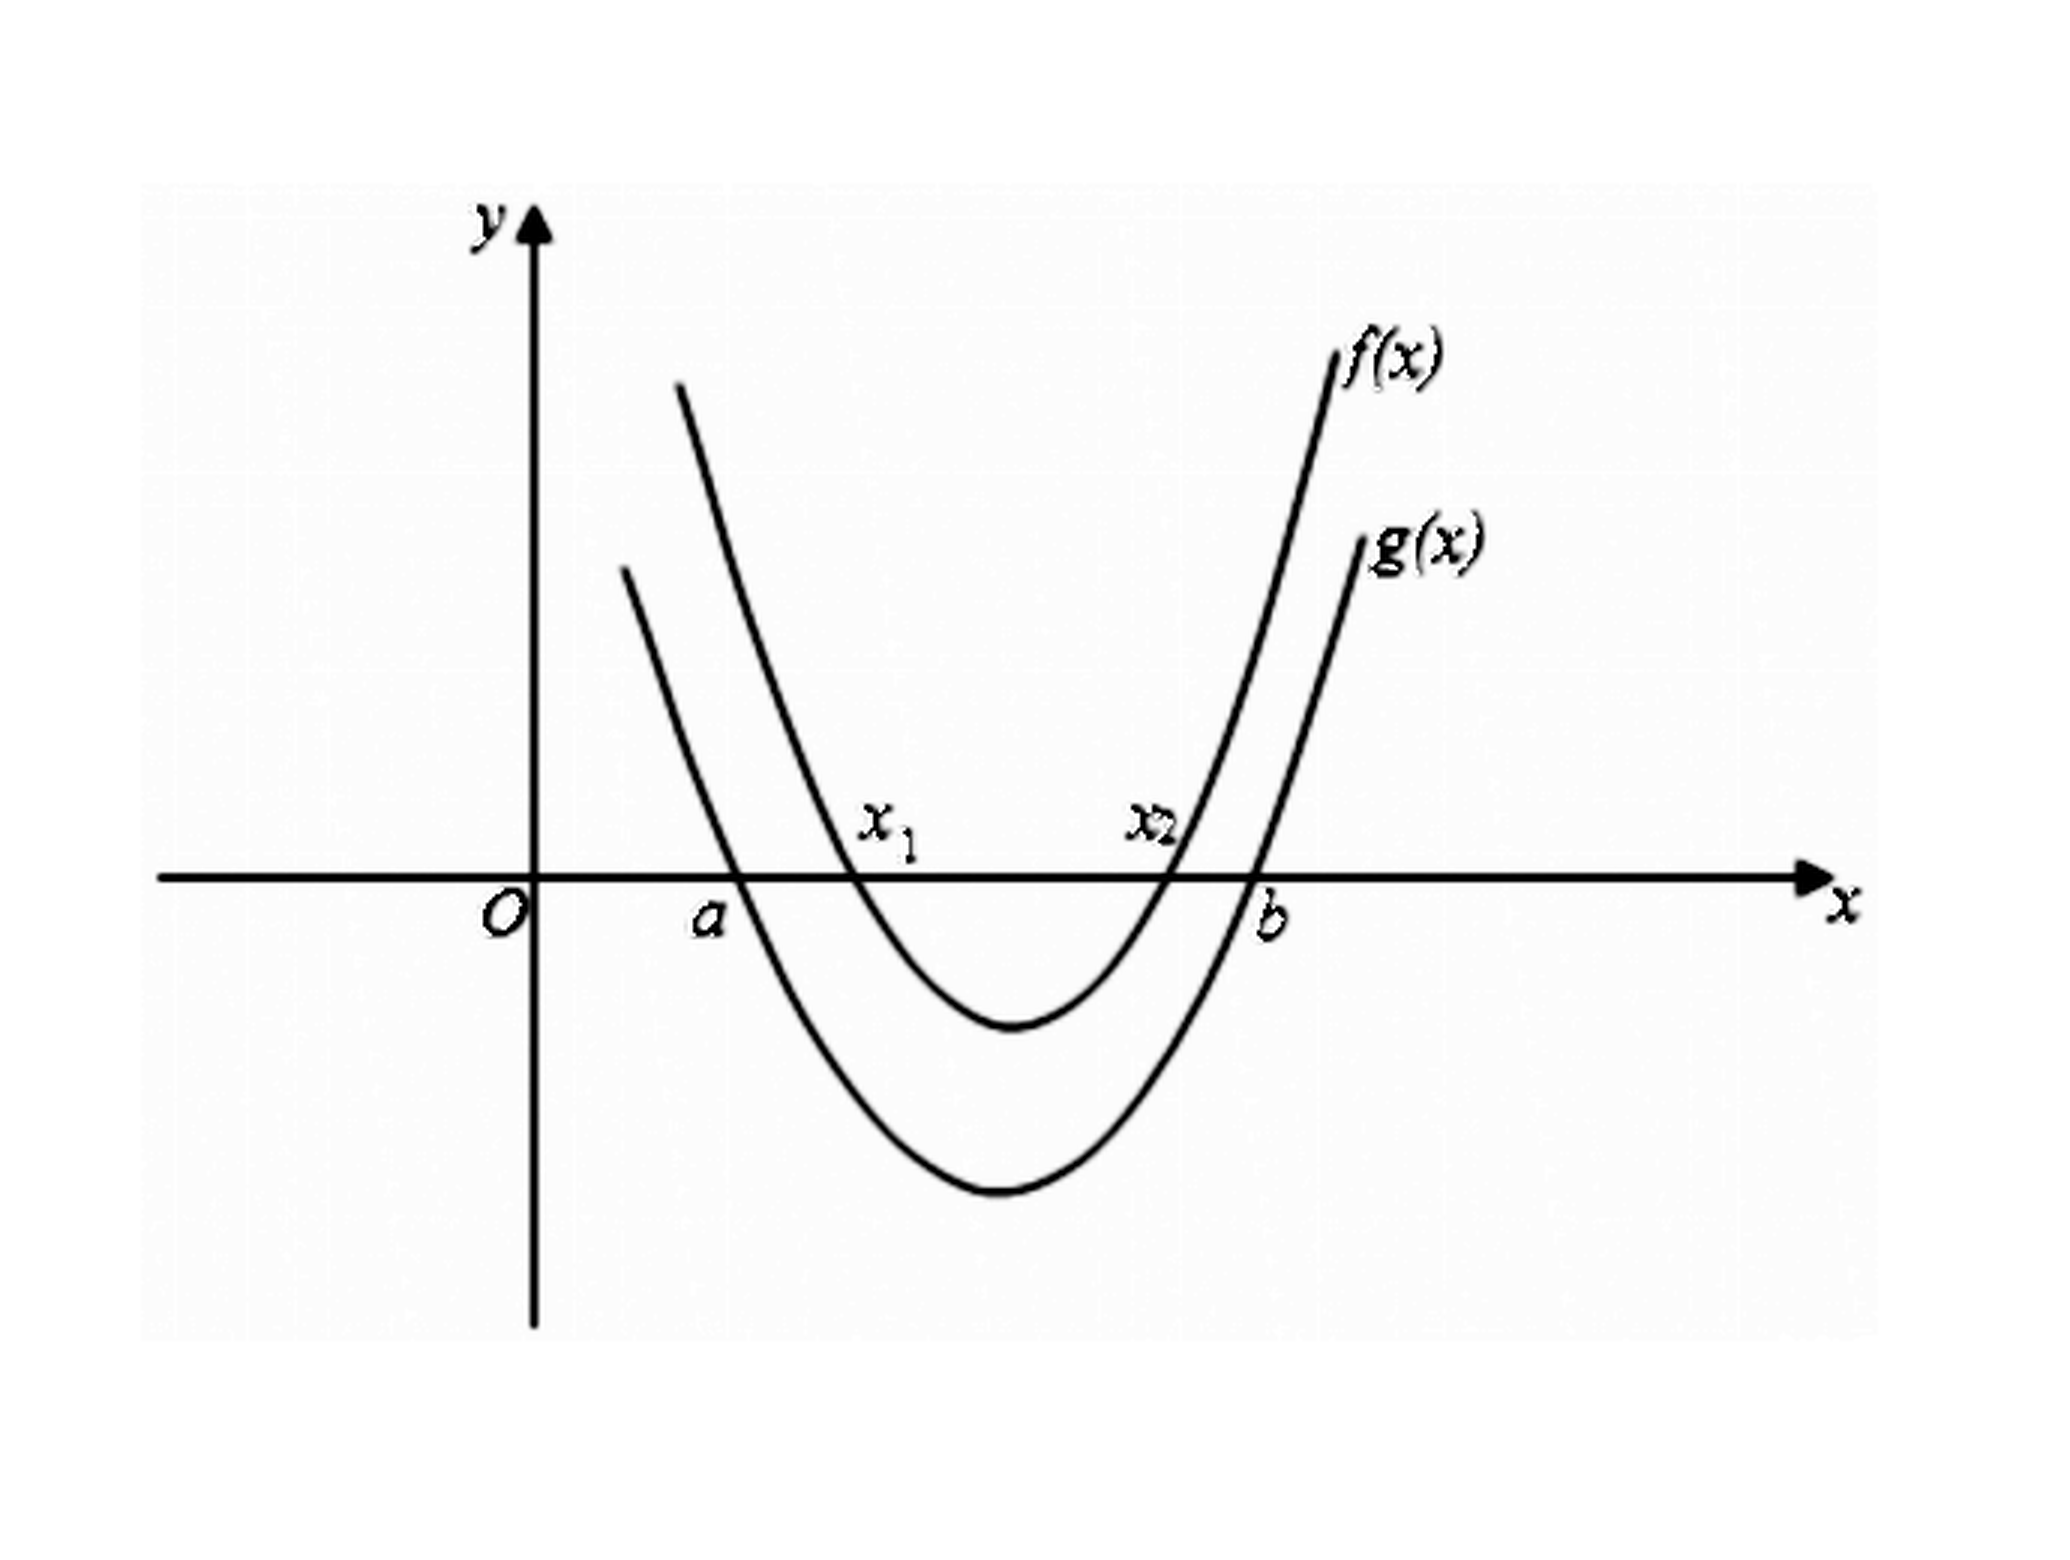
\includegraphics[width=0.52\textwidth]{figures/gao157_q16.png}
\end{center}

\step{由图像得 $a<x_1<x_2<b$，故选 $A$.}
\solend
\fi

\end{enumerate}

\bigsec{三、解答题}

\begin{enumerate}
\setcounter{enumi}{16}

% === Q17 === 解析 6 行；\overline{A}、\varnothing、\subseteq 无、cases
\item 设全集为 $\R$，$m\in\R$，集合 $A=\{x\mid 2<x<5\}$，$B=\{x\mid 2m\leqslant x\leqslant 5m-3\}$.

(1) 若 $m=2$，求 $\overline{A}\cup B$；

(2) 若 $A\cap B=B$，求 $m$ 的取值范围.

\ifanswer
\solbegin
\step{(1) $\overline{A}=\{x\mid x\leqslant2$ 或 $x\geqslant5\}$，当 $m=2$ 时，$B=\{x\mid 4\leqslant x\leqslant7\}$，}
\step{则 $\overline{A}\cup B=\{x\mid x\leqslant2$ 或 $x\geqslant4\}$；}
\step{(2) 因为 $A\cap B=B$，所以 $B$ 是 $A$ 的子集，}
\step{当 $B=\varnothing$ 时，$2m>5m-3$，解得 $m<1$；}
\step{当 $B\ne\varnothing$ 时，$\begin{cases}2m\leqslant5m-3\\2m>2\\5m-3<5\end{cases}$，解得 $1<m<\dfrac85$；}
\step{综上，$m$ 的取值范围是 $(-\infty,1)\cup\left(1,\dfrac85\right)$.}
\solend
\fi

% === Q18 === 解析 2 行；指数式、\lg、换底
\item (1) 设 $a^{2x}=3$，且 $a>0$，求 $\dfrac{a^{3x}+a^{-3x}}{a^x+a^{-x}}$ 的值；

(2) 已知 $\lg2=a, 10^b=3$，用 $a$ 及 $b$ 表示 $\log_{12}25$.

\ifanswer
\solbegin
\step{(1) $\dfrac{a^{3x}+a^{-3x}}{a^x+a^{-x}}=a^{2x}-1+a^{-2x}=3-1+\dfrac13=\dfrac73$；}
\step{(2) $\log_{12}25=\dfrac{\lg25}{\lg12}=\dfrac{2-2\lg2}{2\lg2+\lg3}=\dfrac{2-2a}{2a+b}$.}
\solend
\fi

% === Q19 === 解析 11 行；幂函数、$=0$ 笔误照录、\Delta、\sqrt5、cases
\item 已知幂函数 $f(x)=(m^2+m-1)x^{-2m^2+m+3}$ 在 $(0,+\infty)$ 上为严格增函数.

(1) 求 $f(x)$ 的解析式；

(2) 若 $k+kf(x)>f(x)-x-1$ 对任意实数 $x$ 都成立，求实数 $k$ 的取值范围；

(3) 若关于 $x$ 的不等式 $f(x)\leqslant8x-a$ 的解集中有且仅有 $5$ 个整数，求实数 $a$ 的范围.

\ifanswer
\solbegin
\step{(1) 由题意得 $m^2+m-1=1$，且 $-2m^2+m+3>0$，}
\step{解得 $m=-2$（舍去）或 $m=1$，所以 $f(x)=x^2$；}
\step{(2) $k+kf(x)>f(x)-x-1$ 可化为 $(k-1)x^2+x+k+1=0$ 恒成立，}
\step{当 $k=1$ 时，$x+2>0$，显然不恒成立；}
\step{当 $k\ne1$ 时，要使该二次不等式恒成立，只需 $\begin{cases}k-1>0\\[2pt]\Delta=1-4(k+1)(k-1)\leqslant0\end{cases}$，}
\step{解得 $k\geqslant\dfrac{\sqrt5}{2}$，即所求 $k$ 的范围是 $\left[\dfrac{\sqrt5}{2},+\infty\right)$；}
\step{(3) 不等式 $f(x)\leqslant8x-a$，即 $x^2-8x+a\leqslant0$ 有五个整数解，}
\step{令 $g(x)=x^2-8x+a$，因为该函数开口向上，对称轴为 $x=4$，}
\step{所以解集内的整数为 $2$，$3$，$4$，$5$，$6$，}
\step{由二次函数的性质得，只需 $\begin{cases}g(1)=1-8+a>0\\g(2)=4-8\times2+a\leqslant0\end{cases}$，解得 $7<a\leqslant12$，}
\step{故 $a$ 的取值范围是 $(7,12]$.}
\solend
\fi

% === Q20 === 解析 12 行；材料题、$a+b=1$、大根号、"因出"笔误、分母套分数
\item 问题：正数 $a$、$b$ 满足 $a+b=1$，求 $\dfrac1a+\dfrac2b$ 的最小值.

其中一种解法是：$\dfrac1a+\dfrac2b=\left(\dfrac1a+\dfrac2b\right)(a+b)=1+\dfrac ba+\dfrac{2a}{b}+2\geqslant3+2\sqrt2$，

当且仅当 $\dfrac ba=\dfrac{2a}{b}$ 且 $a+b=1$ 时，即 $a=\sqrt2-1$ 且 $b=2-\sqrt2$ 时取等号.

学习上述解法并解决下列问题：

(1) 若正实数 $x$、$y$ 满足 $x+y=1$，求 $\dfrac2x+\dfrac1y$ 的最小值；

(2) 若实数 $a$、$b$、$x$、$y$ 满足 $\dfrac{x^2}{a^2}-\dfrac{y^2}{b^2}=1$，求证：$a^2-b^2\leqslant(x-y)^2$；

(3) 利用 (2) 的结论，求代数式 $M=\sqrt{2m-5}-\sqrt{m-3}$ 的最小值，并求出使得 $M$ 最小的 $m$ 的值.

\ifanswer
\solbegin
\step{(1) $\dfrac2x+\dfrac1y=(x+y)\left(\dfrac2x+\dfrac1y\right)=3+\dfrac xy+\dfrac{2y}{x}\geqslant3+2\sqrt2$，}
\step{当且仅当 $\dfrac xy=\dfrac{2y}{x}$ 且 $x+y=1$ 时取等号；}
\step{(2) $a^2-b^2=(a^2-b^2)\left(\dfrac{x^2}{a^2}-\dfrac{y^2}{b^2}\right)=x^2+y^2-\left(\dfrac{a^2x^2}{b^2}+\dfrac{b^2y^2}{a^2}\right)$}
\step{$\leqslant x^2+y^2-2\sqrt{\dfrac{a^2x^2}{b^2}\cdot\dfrac{b^2y^2}{a^2}}=x^2+y^2-2xy=(x-y)^2$，}
\step{故当 $b^4x^2=a^4y^2$ 时，等号成立.}
\step{(3) 令 $x=\sqrt{2m-5}, y=\sqrt{m-3}$，由 $\begin{cases}2m-5\geqslant0\\m-3\geqslant0\end{cases}$ 得 $m\geqslant3$，}
\step{$x^2-y^2=(2m-5)-(m-3)=m-2>0$，}
\step{又 $x>0, y>0$，所以 $x>y$，所以 $\dfrac{x^2}{a^2}-\dfrac{y^2}{b^2}=1$，}
\step{由 $x^2-2y^2=1$，得 $\dfrac{x^2}{1}-\dfrac{y^2}{\frac12}=1$，因出 $a^2=1, b^2=\dfrac12$，}
\step{由 (2) 得 $M=\sqrt{2m-5}-\sqrt{m-3}=x-y\geqslant\sqrt{a^2-b^2}=\sqrt{1-\dfrac12}=\dfrac{\sqrt2}{2}$，}
\step{当且仅当 $\dfrac xy=\left(\dfrac ab\right)^2=2$ 取等号，结合 $x^2-2y^2=1$，解得 $x=\sqrt2, y=\dfrac{\sqrt2}{2}$，}
\step{即 $\sqrt{2m-5}=\sqrt2$，得 $m=\dfrac72$，所以 $m=\dfrac72$ 时，$M$ 取得最小值 $\dfrac{\sqrt2}{2}$.}
\solend
\fi

\end{enumerate}

\end{document}
"
%
% ① 原始材料：微信公众号"魔都数学加油站"文章，连载"27学年高一157"，原文标题
% "27学年高一157——2026-2027年上海市大境中学高一上期中"；
% 原文链接：https://mp.weixin.qq.com/s/s6eDMDVkxc2fcBe8LNm-Tw 。
% 正文为 8 张 PNG 页（01/02/03/04/06 为 4762×6735，05/07/08 为 2560×3620，
% 同一篇各页分辨率混排，逐页按各自分辨率裁图核对）。
% 体例：讲评版——填空 3—12（10 题）、选择 13—16（4 题）、解答 17—20（4 题），
% 共 18 题，自第 3 题起编（1、2 未印在本篇）；末题是第 20 题（不是 21）。
% 除第 4 题只印【答案】外，其余 17 题逐题印【解析】（逐题核实，见 ②）。
% 题目、答案、解析均据原图转录；卷面粉红色水印"魔都数学加油站"及公众号
% 页脚未录入。
% 全卷仅 1 幅配图：第 16 题解析内函数图像（"设 g(x)=(x-a)(x-b)，
% f(x)=g(x)+1，画出函数 g(x) 与函数 f(x) 的图像，如图所示"），
% 解析内配图仅答案版出，裁 figures/gao157_q16.png；逐页通读 8 页确认
% 无题目配图、无表格；08 页下半仅水印、无正文。
%
% 卷首标题：原卷印作"2026-2027 年大境中学高一上期中"，年份区间按全稿惯例排 en dash；
% 原卷卷面未印副标题，本稿按同期中卷知识模块口径补出"集合与常用逻辑用语、不等式、函数"。
%
% ② 与原卷的排版差异：
%   ① 原文从第 3 题起，本稿保留原题号；共 18 题三节，解答题 4 题到 20；
%      三节各自 \begin{enumerate}…\end{enumerate} + \setcounter{enumi}{2/12/16}
%      （题目溯源.py 按 \bigsec 切节、每节独立计 depth，只收 depth==1 的 \item，
%       见 高一156 头注②的订正）；
%   ② 第 4 题只印【答案】、无【解析】，提 \ans{}；其余 17 题逐题印【解析】、
%      逐题设 \solbegin…\solend；四道选择题答案在解析末句"故选 D／D／C／A"
%      （逐个放大复核）、括号 \mbox{（\quad）} 留空；答案版【答案】/【解析】
%      标记数 = 18 = 全卷题数（1 个 \ans ＋ 17 个 \solbegin）；
%   ③ 原卷卷面未印副标题，本稿按知识模块口径补出；
%   ④ 原卷填空横线按全稿惯例排 \blankline[4.4em]；选择题选项段前按惯例各加
%      \keepwithprev；解答题不留作答区、不加 \anspace（原卷为讲评版，109—113 起
%      全稿不用 \anspace）；
%   ⑤ 数集：Q4"$x、y\in R$"、Q6"$x\in R$"、Q10"$a\in Z$"、Q12"$n\in Z$"
%      "$n_1、n_2\in Z$"、Q17"全集为 R／$m\in R$"原卷印斜体 R/Z，按全稿惯例
%      归一 \R／\Z（参见 高一14 头注④、高一150 头注②⑤、高一153 头注⑤）；
%      绝对值排 \lvert…\rvert（Q6 $\lvert x-1\rvert$／$\lvert x+3\rvert$／
%      $\lvert 2x+2\rvert$），集合描述竖线排 \mid（Q12、Q17），空集 \varnothing
%      （Q17"$B=\varnothing$"），补集照原卷上划线排 \overline{A}（Q17），
%      不等号按全稿惯例排 \leqslant／\geqslant；
%   ⑥ 判别式三处（Q8"$\Delta=(-2m)^2-4(m+2)$"、Q15"$\Delta=(a+2)^2+4(a^2-4)<0$"、
%      Q19"$\Delta=1-4(k+1)(k-1)\leqslant0$"）放大比对同形、均为等腰偏高且右斜边
%      加粗的 \Delta，统一照录 \Delta；本卷无扁三角 \triangle 用例（与 高一142／
%      高一151／高一152 的 Δ/△ 混用卷不同）；
%   ⑦ "图像／图象"逐处照录不统一：Q9"图像过点 $(4,2)$""它的图像过点"、
%      Q16"画出函数 $g(x)$ 与函数 $f(x)$ 的图像""由图像得"用"图像"；
%      Q14 题干及解析四处均用"图象"（"的图象关于原点对称""图象关于 $y$ 轴对称"）；
%   ⑧ 原卷笔误／未化简式照录：
%      · Q5 解析"$2\sqrt4+1=5$"根号 4 原卷未化简，照录 \sqrt4；
%      · Q7 解析"$\lg\frac{E_1}{E_2}=\frac25\cdot(m_2-m_1)=\frac25(-1.45+26.7)=10.1$"
%        第一处有 \cdot、第二处无，逐处照录；题干"$m_1-m_2=-\frac52\lg\frac{E_1}{E_2}$"；
%      · Q10 解析"$f(1)=\frac{a+1}{1+2}\geqslant0$"与 cases 第二行分母均印 $1+2$、
%        未化简成 $3$，照录；
%      · Q19 (2)"可化为 $(k-1)x^2+x+k+1=0$ 恒成立"原卷印 $=0$（与 >0 恒成立
%        的题意不符），照录笔误；
%      · Q20 (3)"因出 $a^2=1, b^2=\frac12$"原卷印"因出"（当作"因此"），照录；
%      · Q20 (3)"得 $\frac{x^2}{1}-\frac{y^2}{\frac12}=1$"分母套分数、照录；
%   ⑨ 圈数字①②在文本模式（Q15 解析"①当 $a^2-4=0$ 时""②当 $a^2-4\ne0$ 时"，
%      共 2 枚）；子题标号 (1)(2)(3) 半角括号照录；行末西文句点 ASCII `.`；
%      行中全角逗号／顿号照录；半角逗号在数学组之间是全稿惯例、非笔误
%      （Q8"$x_1+x_2=2m, x_1x_2=m+2$"、Q12"$n\in Z$"、Q18"$\lg2=a, 10^b=3$"、
%      Q20"$a^2=1, b^2=\frac12$"等）；中文弯引号""照录（Q4 命题）；
%   ⑩ 自定义名词：Q11"交叉数"、Q12"$a\otimes b$"新定义运算、Q20"问题／
%      其中一种解法是／学习上述解法并解决下列问题"材料题，均照原卷录入；
%   ⑪ 配图：全卷 1 幅（逐页通读 8 页确认）——Q16 解析内函数图像（05 页右侧，
%      $f(x)$ 与 $g(x)$ 两条抛物线、标注 $a,x_1,x_2,b$），仅答案版出，
%      裁 figures/gao157_q16.png，去粉色水印、去色、3× LANCZOS 放大；
%      图放 \ifanswer 内 \solbegin…\solend 的两 \step 之间（高一108 第 6 题／
%      高一156 Q15 成例）；Q16 题干无"如图"、不需题目配图守卫。
%
% ③ 行数复核：一条 \step = 原卷解析的一个印刷行，cases 块作一个印刷行计；
%    跨半页重叠行（Q5 的"【解析】x-1>0…"、Q10 的"所以 a=-1 或 a=0"、
%    Q12 的"【解析】由 u⊗v…"、Q14 的"f(x)=x² 图象关于 y 轴对称"、
%    Q19 的"(1) 由题意得…"、Q20 的"(3) 令 x=…"等 hi_1/hi_2 两半页共有的行）
%    只计一次，别把原卷折行并起来。
%    逐题数（主会话逐页核对定稿）：Q3：1；Q4：0（只印【答案】、提 \ans{}，
%    不计入 \step 账）；Q5：2；Q6：5；Q7：2；Q8：5；Q9：3；Q10：4；
%    Q11：3；Q12：6；Q13：3；Q14：5；Q15：9；Q16：4；Q17：6；Q18：2；
%    Q19：11；Q20：12。合计 83 条 \step（本卷无 \stepm），与原卷逐题印刷行相等。
%    全卷 18 题：1 题只印【答案】（\ans）、17 题印【解析】（\solbegin…\solend），
%    答案版【答案】/【解析】标记数 = 18 = 全卷题数。
%    全卷除此 6 类外未发现其它笔误／自相矛盾处；17 题印【解析】、1 题印【答案】。
%
\documentclass[a4paper,11pt]{article}
\usepackage{common}

\begin{document}

\examtitlest[3]{2026--2027 年大境中学高一上期中}{集合与常用逻辑用语、不等式、函数}

\bigsec{一、填空题}

\begin{enumerate}
\setcounter{enumi}{2}

% === Q3 === 解析 1 行；$a,b$ 半角逗号照录
\item 若 $a=x^2-2x+1$，$b=x-3$，则 $a,b$ 的大小关系为\blankline[4.4em].

\ifanswer
\solbegin
\step{$a-b=x^2-3x+4=\left(x-\dfrac32\right)^2+\dfrac74>0$，所以 $a>b$.}
\solend
\fi

% === Q4 === 只印【答案】、无【解析】；中文弯引号、\R、顿号；提 \ans{}
\item 用反证法证明命题：“设 $x$、$y\in\R$. 若 $x+y>2$，则 $x>1$ 或 $y>1$”时，假设的内容应该是\blankline[4.4em].

\ifanswer
\ans{$x\leqslant1$ 且 $y\leqslant1$}
\fi

% === Q5 === 解析 2 行；$2\sqrt4+1=5$ 根号 4 未化简照录
\item 当 $x>1$ 时，$x+\dfrac4{x-1}$ 的最小值为\blankline[4.4em].

\ifanswer
\solbegin
\step{$x-1>0$，$x+\dfrac4{x-1}=(x-1)+\dfrac4{x-1}+1\geqslant2\sqrt4+1=5$，}
\step{当且仅当 $x-1=\dfrac4{x-1}$，即 $x=3$ 时取等号，故最小值为 $5$.}
\solend
\fi

% === Q6 === 解析 5 行；绝对值 \lvert…\rvert、\cup、\R
\item 设 $x\in\R$，方程 $\lvert x-1\rvert+\lvert x+3\rvert=\lvert 2x+2\rvert$ 的解集是\blankline[4.4em].

\ifanswer
\solbegin
\step{当 $x\leqslant-3$ 时，方程为 $1-x-x-3=-2x-2$，等式成立；}
\step{当 $-3<x\leqslant-1$ 时，方程为 $1-x+x+3=-2x-2$，解得 $x=-3$，舍去；}
\step{当 $-1<x<1$ 时，方程为 $1-x+x+3=2x+2$，解得 $x=1$，舍去；}
\step{当 $x\geqslant1$ 时，方程为 $x-1+x+3=2x+2$，等式成立，}
\step{综上，方程 $\lvert x-1\rvert+\lvert x+3\rvert=\lvert 2x+2\rvert$ 的解集为 $(-\infty,-3]\cup[1,+\infty)$.}
\solend
\fi

% === Q7 === 解析 2 行；星等材料题、\lg、\cdot 逐处照录、天狼星
\item 在天文学中，天体的明暗程度可以用星等或亮度来描述，两颗星的星等与亮度满足 $m_1-m_2=-\dfrac52\lg\dfrac{E_1}{E_2}$，其中星等为 $m_k$ 的星的亮度为 $E_k(k=1,2)$. 已知太阳的星等为 $-26.7$，天狼星的星等为 $-1.45$，则太阳与天狼星的亮度的比值为\blankline[4.4em].

\ifanswer
\solbegin
\step{两颗星的星等与亮度满足 $m_1-m_2=-\dfrac52\lg\dfrac{E_1}{E_2}$，令 $m_2=-1.45$，$m_1=-26.7$，}
\step{$\lg\dfrac{E_1}{E_2}=\dfrac25\cdot(m_2-m_1)=\dfrac25(-1.45+26.7)=10.1$，$\dfrac{E_1}{E_2}=10^{10.1}$.}
\solend
\fi

% === Q8 === 解析 5 行；韦达定理、判别式 \Delta、半角逗号在数学组间
\item 已知方程 $x^2-2mx+m+2=0$ 有两个实数根 $x_1,x_2$，满足 $x_1^2+x_2^2=2$，则实数 $m$ 的值为\blankline[4.4em].

\ifanswer
\solbegin
\step{对于方程 $x^2-2mx+m+2=0$，由韦达定理得 $x_1+x_2=2m, x_1x_2=m+2$，}
\step{又 $x_1^2+x_2^2=(x_1+x_2)^2-2x_1x_2=(2m)^2-2(m+2)=4m^2-2m-4=2$，}
\step{解得 $m=\dfrac32$ 或 $m=-1$，}
\step{因为方程有两个实数根，所以 $\Delta=(-2m)^2-4(m+2)=4m^2-4m-8\geqslant0$，}
\step{解得 $m\leqslant-1$ 或 $m\geqslant2$，故 $m=-1$.}
\solend
\fi

% === Q9 === 解析 3 行；"图像"照录、$x^\alpha$、$x^{1/2}=\sqrt{x}$
\item 已知幂函数 $y=f(x)$ 的图像过点 $(4,2)$，则不等式 $f(x^2-2x)<f(2-x)$ 的解集为\blankline[4.4em].

\ifanswer
\solbegin
\step{设幂函数 $y=f(x)=x^\alpha$，它的图像过点 $(4,2)$，所以 $4^\alpha=2$，$\alpha=\dfrac12$，}
\step{故 $f(x)=x^{\frac12}=\sqrt{x}$，由不等式 $f(x^2-2x)<f(2-x)$，}
\step{得 $0\leqslant x^2-2x<2-x$，得 $-1<x\leqslant0$，故解集为 $(-1,0]$.}
\solend
\fi

% === Q10 === 解析 4 行；$a\in\Z$、cases（分母 $1+2$ 未化简）、参数分离
\item 已知函数 $y=\dfrac{ax+1}{x+2}$（常数 $a\in\Z$）. 要使该函数在区间 $[1,+\infty)$ 上是严格减函数，并且函数值不恒为负，则满足条件的 $a$ 的取值为\blankline[4.4em].

\ifanswer
\solbegin
\step{函数参数分离为 $y=\dfrac{a(x+2)+1-2a}{x+2}=a+\dfrac{1-2a}{x+2}$，}
\step{若函数在区间 $[1,+\infty)$ 上严格减函数，则 $1-2a>0$，}
\step{且函数的最大值 $f(1)=\dfrac{a+1}{1+2}\geqslant0$，即 $\begin{cases}1-2a>0\\[2pt]\dfrac{a+1}{1+2}\geqslant0\end{cases}$，解得 $-1\leqslant a<\dfrac12$，又 $a\in\Z$，}
\step{所以 $a=-1$ 或 $a=0$.}
\solend
\fi

% === Q11 === 解析 3 行；"交叉数"自定义名词、$(-1)^t$、$2^5$、$32\times3=96$
\item 对非空集合 $A$ 中的每个元素 $t$，都乘以 $(-1)^t$ 再求和，称为集合 $A$ 的交叉数，例如 $A=\{2,3,6\}$，则集合 $A$ 的交叉数为 $(-1)^2\cdot2+(-1)^3\cdot3+(-1)^6\cdot6=5$. 若集合 $W=\{1,2,3,4,5,6\}$，则 $W$ 的所有非空子集的交叉数的总和为\blankline[4.4em].

\ifanswer
\solbegin
\step{固定 $W$ 中的任一元素，其余 $5$ 个元素各有选或不选两种情况，}
\step{因此该元素出现在 $2^5$ 个非空子集中，}
\step{所有交叉数的总和为 $2^5(-1+2-3+4-5+6)=32\times3=96$.}
\solend
\fi

% === Q12 === 解析 6 行；\otimes、\lambda、\mid、\Z、\times 与 \cdot 逐处照录
\item 对于任意两个正实数 $a$、$b$，定义 $a\otimes b=\lambda\cdot\dfrac ab$，其中常数 $\lambda\in\left(\dfrac{\sqrt2}{2},1\right)$. 若 $u\geqslant v>0$，且 $u\otimes v$ 与 $v\otimes u$ 都是集合 $\left\{x\mid x=\dfrac n2,n\in\Z\right\}$ 的元素，则 $u\otimes v=$\blankline[4.4em].

\ifanswer
\solbegin
\step{由 $u\otimes v$ 与 $v\otimes u$ 都是集合 $\left\{x\mid x=\dfrac n2,n\in\Z\right\}$ 的元素，}
\step{不妨设 $\lambda\times\dfrac uv=\dfrac12 n_1$，$\lambda\times\dfrac vu=\dfrac12 n_2$，$n_1$、$n_2\in\Z$，}
\step{因为 $u\geqslant v>0$，所以 $0<\dfrac vu\leqslant1$，因为 $\lambda\in\left(\dfrac{\sqrt2}{2},1\right)$，所以 $\dfrac12 n_2=\lambda\cdot\dfrac vu\in(0,1)$，}
\step{因为 $n_2\in\Z$，所以 $n_2=1$，即 $\dfrac12=\dfrac{\lambda v}{u}$，所以 $\lambda=\dfrac{u}{2v}\in\left(\dfrac{\sqrt2}{2},1\right)$，}
\step{所以 $\dfrac uv\in(\sqrt2,2)$，$\dfrac{u^2}{v^2}\in(2,4)$，则 $\lambda\cdot\dfrac uv=\dfrac{u^2}{v^2}\times\dfrac12=\dfrac12 n_1\in(1,2)$，}
\step{因为 $n_1\in\Z$，所以 $n_1=3$，$\dfrac12 n_1=\dfrac32$，故 $u\otimes v=\dfrac32$.}
\solend
\fi

\end{enumerate}

\bigsec{二、选择题}

\begin{enumerate}
\setcounter{enumi}{12}

% === Q13 === 解析 3 行；选项段 \keepwithprev；故选 D
\item 下列不等式成立的为\mbox{（\quad）}

\keepwithprev
A. 若 $a>b$，则 $ac^2>bc^2$\qquad B. 若 $a>b$，则 $a^2>b^2$

C. 若 $a>b$，$c>d$，则 $a+b>c+d$\qquad D. 若 $a>b$，则 $a^3>b^3$

\ifanswer
\solbegin
\step{A 中 $c=0$ 时不成立；B 取 $a=1$，$b=-2$ 不成立；}
\step{C 取 $a=1$，$b=0$，$c=5$，$d=0$ 不成立.}
\step{幂函数 $y=x^3$ 在实数集上严格递增，所以 $a>b\Rightarrow a^3>b^3$，故选 $D$.}
\solend
\fi

% === Q14 === 解析 5 行；"图象"四处照录；故选 D
\item 幂函数 $f(x)=x^\alpha$ 的图象关于原点对称，且在 $(-\infty,0)$ 上是严格增函数，则 $f(x)$ 可以是\mbox{（\quad）}

\keepwithprev
A. $f(x)=x^{-1}$\qquad B. $f(x)=x^{\frac12}$\qquad C. $f(x)=x^2$\qquad D. $f(x)=x^3$

\ifanswer
\solbegin
\step{$f(x)=\dfrac1x$ 的图象关于原点对称，在 $(-\infty,0)$ 上是严格减函数，故 $A$ 错误；}
\step{$f(x)=x^{\frac12}$ 在 $(-\infty,0)$ 上无意义，故 $B$ 错误；}
\step{$f(x)=x^2$ 图象关于 $y$ 轴对称，故 $C$ 错误；}
\step{$f(x)=x^3$ 的图象关于原点对称，且在 $(-\infty,0)$ 上是严格增函数，故 $D$ 正确.}
\step{故选 $D$.}
\solend
\fi

% === Q15 === 解析 9 行；圈数字①②、\Delta、cases；故选 C
\item 若关于 $x$ 的不等式 $(a^2-4)x^2+(a+2)x-1\geqslant0$ 的解集不为空集，则实数 $a$ 的取值范围为\mbox{（\quad）}

\keepwithprev
A. $\left(-2,\dfrac65\right]$\qquad B. $\left[-2,\dfrac65\right]$

C. $(-\infty,-2)\cup\left[\dfrac65,+\infty\right)$\qquad D. $(-\infty,-2]\cup\left[\dfrac65,+\infty\right)$

\ifanswer
\solbegin
\step{①当 $a^2-4=0$ 时，$a=\pm2$，}
\step{若 $a=2$ 时，原不等式为 $4x-1\geqslant0$，则不等式的解集不是空集；}
\step{若 $a=-2$ 时，原不等式为 $-1\geqslant0$，无解，不符合题意；}
\step{②当 $a^2-4\ne0$ 时，$a\ne\pm2$，}
\step{若 $(a^2-4)x^2+(a+2)x-1\geqslant0$ 的解集是空集，则 $\begin{cases}a^2-4<0\\[2pt]\Delta=(a+2)^2+4(a^2-4)<0\end{cases}$，}
\step{解得 $-2<a<\dfrac65$，}
\step{则当不等式 $(a^2-4)x^2+(a+2)x-1\geqslant0$ 的解集不为空集时，}
\step{有 $a<-2$ 或 $a\geqslant\dfrac65$ 且 $a\ne2$，}
\step{综上，实数 $a$ 的取值范围为 $(-\infty,-2)\cup\left[\dfrac65,+\infty\right)$，故选 $C$.}
\solend
\fi

% === Q16 === 解析 4 行＋1 幅解析内配图（仅答案版）；"图像"照录；故选 A
\item 已知实数 $a<b$，关于 $x$ 的不等式 $x^2-(a+b)x+ab+1<0$ 的解集为 $(x_1,x_2)$，则实数 $a$、$b$、$x_1$、$x_2$ 从小到大的排列是\mbox{（\quad）}

\keepwithprev
A. $a<x_1<x_2<b$\qquad B. $x_1<a<b<x_2$\qquad C. $a<x_1<b<x_2$\qquad D. $x_1<a<x_2<b$

\ifanswer
\solbegin
\step{不等式 $x^2-(a+b)x+ab+1<0$ 可化为 $(x-a)(x-b)+1<0$，}
\step{设 $g(x)=(x-a)(x-b)$，$f(x)=g(x)+1$，}
\step{画出函数 $g(x)$ 与函数 $f(x)$ 的图像，如图所示，}

\begin{center}
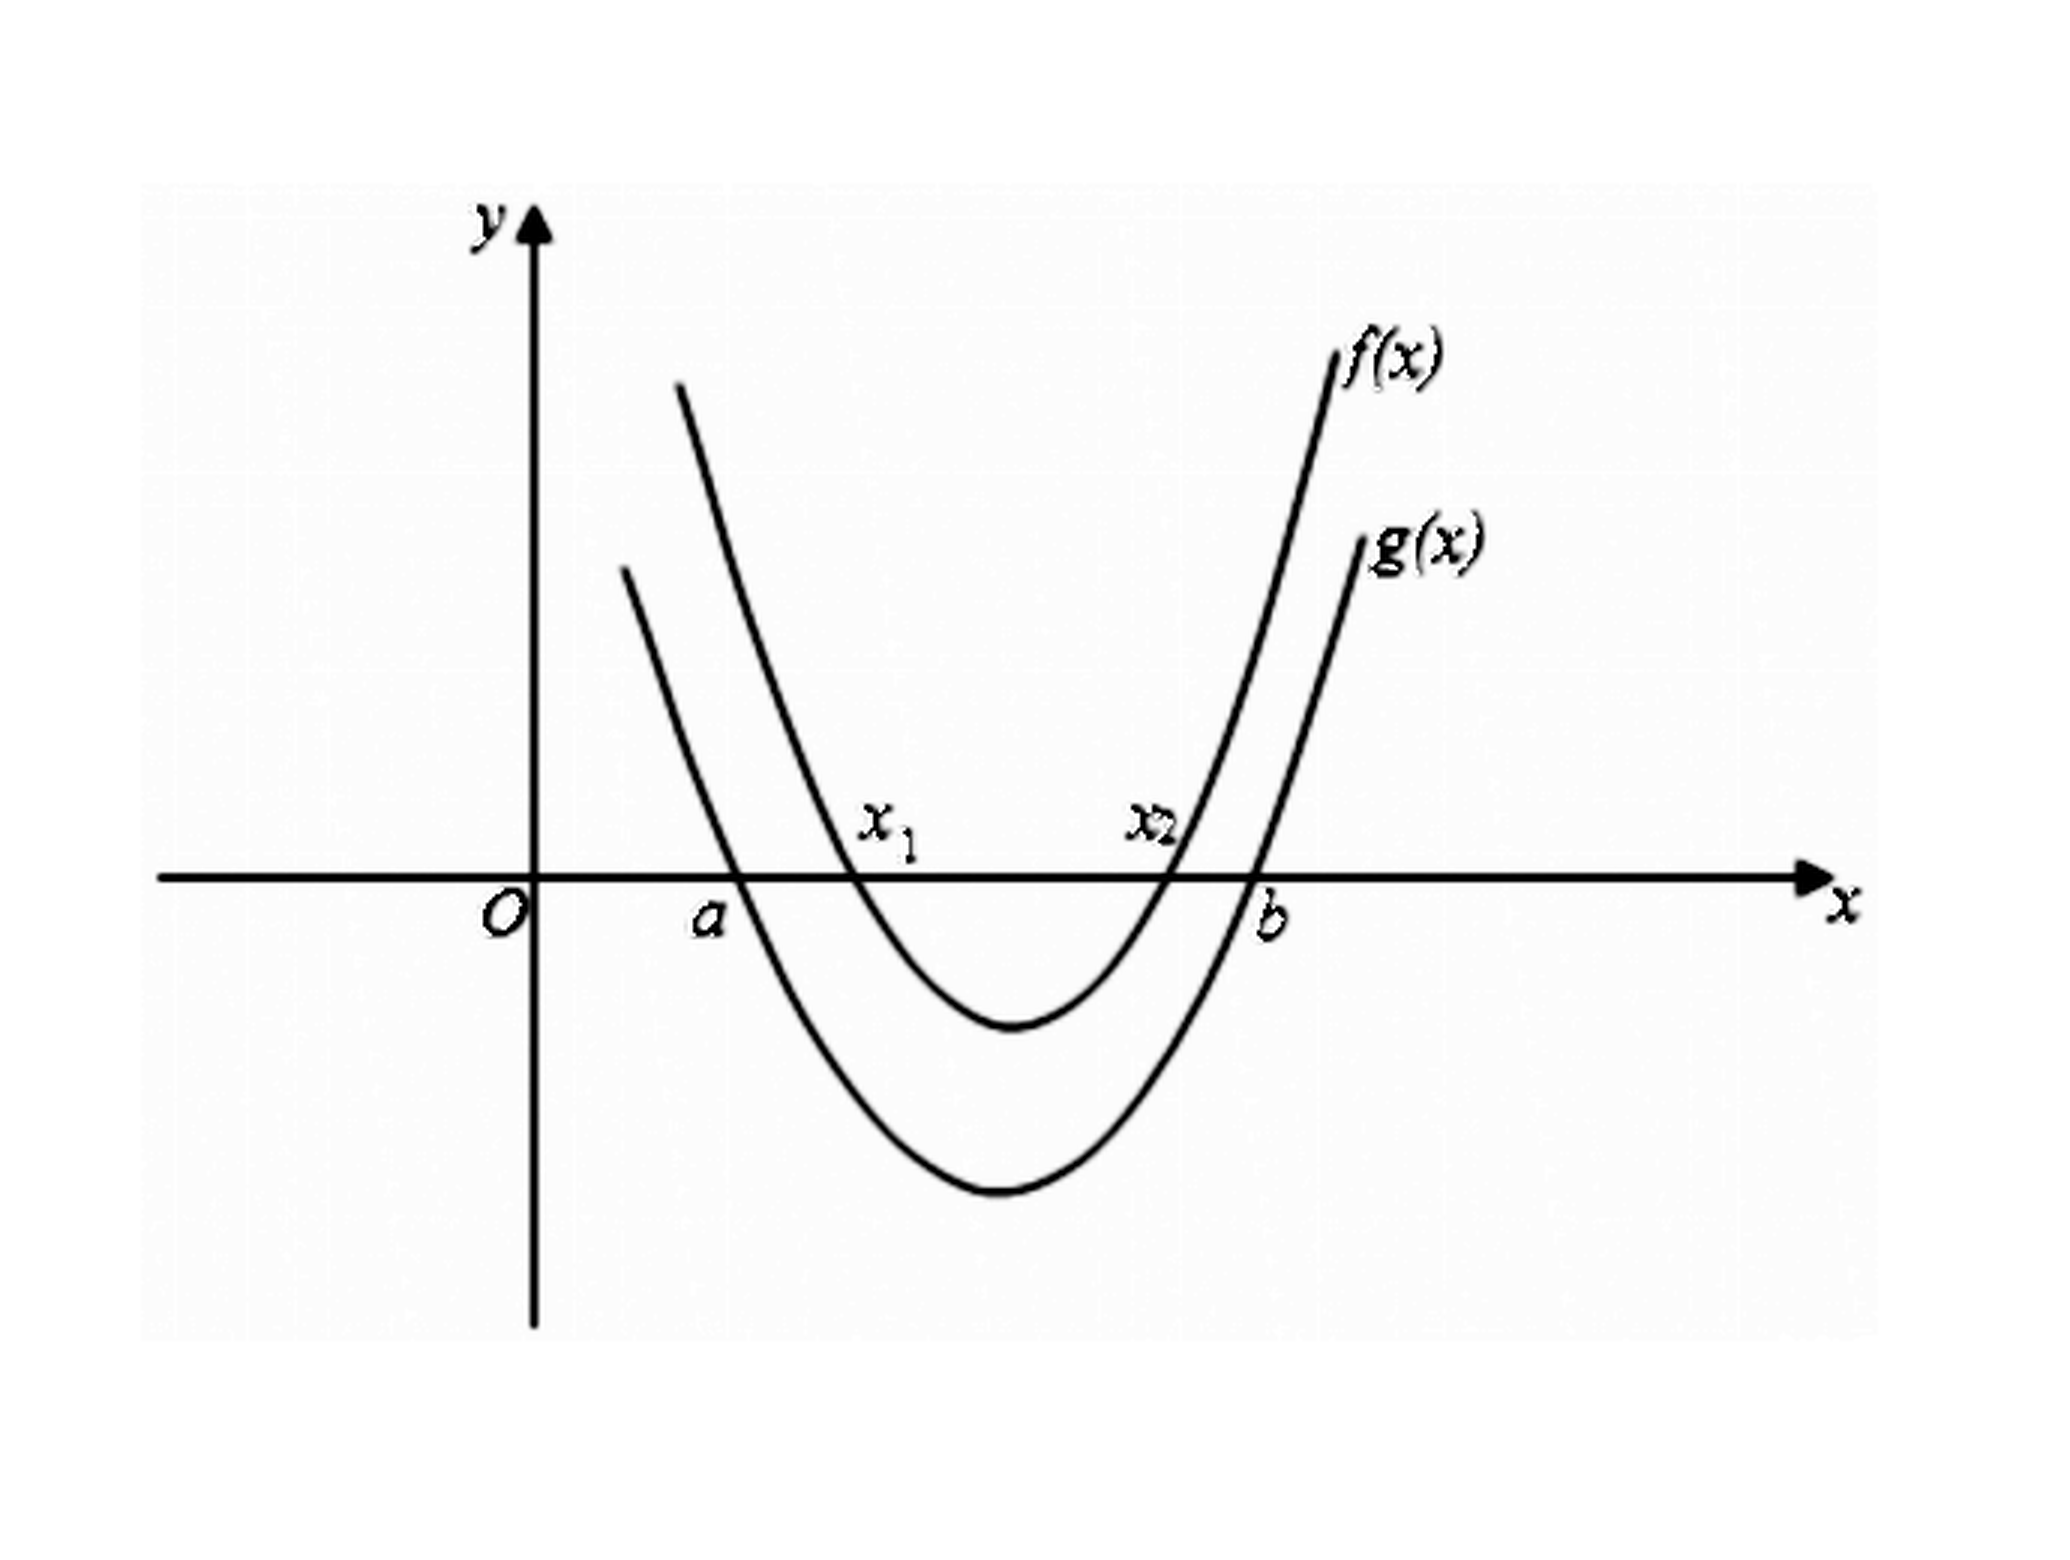
\includegraphics[width=0.52\textwidth]{figures/gao157_q16.png}
\end{center}

\step{由图像得 $a<x_1<x_2<b$，故选 $A$.}
\solend
\fi

\end{enumerate}

\bigsec{三、解答题}

\begin{enumerate}
\setcounter{enumi}{16}

% === Q17 === 解析 6 行；\overline{A}、\varnothing、\subseteq 无、cases
\item 设全集为 $\R$，$m\in\R$，集合 $A=\{x\mid 2<x<5\}$，$B=\{x\mid 2m\leqslant x\leqslant 5m-3\}$.

(1) 若 $m=2$，求 $\overline{A}\cup B$；

(2) 若 $A\cap B=B$，求 $m$ 的取值范围.

\ifanswer
\solbegin
\step{(1) $\overline{A}=\{x\mid x\leqslant2$ 或 $x\geqslant5\}$，当 $m=2$ 时，$B=\{x\mid 4\leqslant x\leqslant7\}$，}
\step{则 $\overline{A}\cup B=\{x\mid x\leqslant2$ 或 $x\geqslant4\}$；}
\step{(2) 因为 $A\cap B=B$，所以 $B$ 是 $A$ 的子集，}
\step{当 $B=\varnothing$ 时，$2m>5m-3$，解得 $m<1$；}
\step{当 $B\ne\varnothing$ 时，$\begin{cases}2m\leqslant5m-3\\2m>2\\5m-3<5\end{cases}$，解得 $1<m<\dfrac85$；}
\step{综上，$m$ 的取值范围是 $(-\infty,1)\cup\left(1,\dfrac85\right)$.}
\solend
\fi

% === Q18 === 解析 2 行；指数式、\lg、换底
\item (1) 设 $a^{2x}=3$，且 $a>0$，求 $\dfrac{a^{3x}+a^{-3x}}{a^x+a^{-x}}$ 的值；

(2) 已知 $\lg2=a, 10^b=3$，用 $a$ 及 $b$ 表示 $\log_{12}25$.

\ifanswer
\solbegin
\step{(1) $\dfrac{a^{3x}+a^{-3x}}{a^x+a^{-x}}=a^{2x}-1+a^{-2x}=3-1+\dfrac13=\dfrac73$；}
\step{(2) $\log_{12}25=\dfrac{\lg25}{\lg12}=\dfrac{2-2\lg2}{2\lg2+\lg3}=\dfrac{2-2a}{2a+b}$.}
\solend
\fi

% === Q19 === 解析 11 行；幂函数、$=0$ 笔误照录、\Delta、\sqrt5、cases
\item 已知幂函数 $f(x)=(m^2+m-1)x^{-2m^2+m+3}$ 在 $(0,+\infty)$ 上为严格增函数.

(1) 求 $f(x)$ 的解析式；

(2) 若 $k+kf(x)>f(x)-x-1$ 对任意实数 $x$ 都成立，求实数 $k$ 的取值范围；

(3) 若关于 $x$ 的不等式 $f(x)\leqslant8x-a$ 的解集中有且仅有 $5$ 个整数，求实数 $a$ 的范围.

\ifanswer
\solbegin
\step{(1) 由题意得 $m^2+m-1=1$，且 $-2m^2+m+3>0$，}
\step{解得 $m=-2$（舍去）或 $m=1$，所以 $f(x)=x^2$；}
\step{(2) $k+kf(x)>f(x)-x-1$ 可化为 $(k-1)x^2+x+k+1=0$ 恒成立，}
\step{当 $k=1$ 时，$x+2>0$，显然不恒成立；}
\step{当 $k\ne1$ 时，要使该二次不等式恒成立，只需 $\begin{cases}k-1>0\\[2pt]\Delta=1-4(k+1)(k-1)\leqslant0\end{cases}$，}
\step{解得 $k\geqslant\dfrac{\sqrt5}{2}$，即所求 $k$ 的范围是 $\left[\dfrac{\sqrt5}{2},+\infty\right)$；}
\step{(3) 不等式 $f(x)\leqslant8x-a$，即 $x^2-8x+a\leqslant0$ 有五个整数解，}
\step{令 $g(x)=x^2-8x+a$，因为该函数开口向上，对称轴为 $x=4$，}
\step{所以解集内的整数为 $2$，$3$，$4$，$5$，$6$，}
\step{由二次函数的性质得，只需 $\begin{cases}g(1)=1-8+a>0\\g(2)=4-8\times2+a\leqslant0\end{cases}$，解得 $7<a\leqslant12$，}
\step{故 $a$ 的取值范围是 $(7,12]$.}
\solend
\fi

% === Q20 === 解析 12 行；材料题、$a+b=1$、大根号、"因出"笔误、分母套分数
\item 问题：正数 $a$、$b$ 满足 $a+b=1$，求 $\dfrac1a+\dfrac2b$ 的最小值.

其中一种解法是：$\dfrac1a+\dfrac2b=\left(\dfrac1a+\dfrac2b\right)(a+b)=1+\dfrac ba+\dfrac{2a}{b}+2\geqslant3+2\sqrt2$，

当且仅当 $\dfrac ba=\dfrac{2a}{b}$ 且 $a+b=1$ 时，即 $a=\sqrt2-1$ 且 $b=2-\sqrt2$ 时取等号.

学习上述解法并解决下列问题：

(1) 若正实数 $x$、$y$ 满足 $x+y=1$，求 $\dfrac2x+\dfrac1y$ 的最小值；

(2) 若实数 $a$、$b$、$x$、$y$ 满足 $\dfrac{x^2}{a^2}-\dfrac{y^2}{b^2}=1$，求证：$a^2-b^2\leqslant(x-y)^2$；

(3) 利用 (2) 的结论，求代数式 $M=\sqrt{2m-5}-\sqrt{m-3}$ 的最小值，并求出使得 $M$ 最小的 $m$ 的值.

\ifanswer
\solbegin
\step{(1) $\dfrac2x+\dfrac1y=(x+y)\left(\dfrac2x+\dfrac1y\right)=3+\dfrac xy+\dfrac{2y}{x}\geqslant3+2\sqrt2$，}
\step{当且仅当 $\dfrac xy=\dfrac{2y}{x}$ 且 $x+y=1$ 时取等号；}
\step{(2) $a^2-b^2=(a^2-b^2)\left(\dfrac{x^2}{a^2}-\dfrac{y^2}{b^2}\right)=x^2+y^2-\left(\dfrac{a^2x^2}{b^2}+\dfrac{b^2y^2}{a^2}\right)$}
\step{$\leqslant x^2+y^2-2\sqrt{\dfrac{a^2x^2}{b^2}\cdot\dfrac{b^2y^2}{a^2}}=x^2+y^2-2xy=(x-y)^2$，}
\step{故当 $b^4x^2=a^4y^2$ 时，等号成立.}
\step{(3) 令 $x=\sqrt{2m-5}, y=\sqrt{m-3}$，由 $\begin{cases}2m-5\geqslant0\\m-3\geqslant0\end{cases}$ 得 $m\geqslant3$，}
\step{$x^2-y^2=(2m-5)-(m-3)=m-2>0$，}
\step{又 $x>0, y>0$，所以 $x>y$，所以 $\dfrac{x^2}{a^2}-\dfrac{y^2}{b^2}=1$，}
\step{由 $x^2-2y^2=1$，得 $\dfrac{x^2}{1}-\dfrac{y^2}{\frac12}=1$，因出 $a^2=1, b^2=\dfrac12$，}
\step{由 (2) 得 $M=\sqrt{2m-5}-\sqrt{m-3}=x-y\geqslant\sqrt{a^2-b^2}=\sqrt{1-\dfrac12}=\dfrac{\sqrt2}{2}$，}
\step{当且仅当 $\dfrac xy=\left(\dfrac ab\right)^2=2$ 取等号，结合 $x^2-2y^2=1$，解得 $x=\sqrt2, y=\dfrac{\sqrt2}{2}$，}
\step{即 $\sqrt{2m-5}=\sqrt2$，得 $m=\dfrac72$，所以 $m=\dfrac72$ 时，$M$ 取得最小值 $\dfrac{\sqrt2}{2}$.}
\solend
\fi

\end{enumerate}

\end{document}
"
%
% ① 原始材料：微信公众号"魔都数学加油站"文章，连载"27学年高一157"，原文标题
% "27学年高一157——2026-2027年上海市大境中学高一上期中"；
% 原文链接：https://mp.weixin.qq.com/s/s6eDMDVkxc2fcBe8LNm-Tw 。
% 正文为 8 张 PNG 页（01/02/03/04/06 为 4762×6735，05/07/08 为 2560×3620，
% 同一篇各页分辨率混排，逐页按各自分辨率裁图核对）。
% 体例：讲评版——填空 3—12（10 题）、选择 13—16（4 题）、解答 17—20（4 题），
% 共 18 题，自第 3 题起编（1、2 未印在本篇）；末题是第 20 题（不是 21）。
% 除第 4 题只印【答案】外，其余 17 题逐题印【解析】（逐题核实，见 ②）。
% 题目、答案、解析均据原图转录；卷面粉红色水印"魔都数学加油站"及公众号
% 页脚未录入。
% 全卷仅 1 幅配图：第 16 题解析内函数图像（"设 g(x)=(x-a)(x-b)，
% f(x)=g(x)+1，画出函数 g(x) 与函数 f(x) 的图像，如图所示"），
% 解析内配图仅答案版出，裁 figures/gao157_q16.png；逐页通读 8 页确认
% 无题目配图、无表格；08 页下半仅水印、无正文。
%
% 卷首标题：原卷印作"2026-2027 年大境中学高一上期中"，年份区间按全稿惯例排 en dash；
% 原卷卷面未印副标题，本稿按同期中卷知识模块口径补出"集合与常用逻辑用语、不等式、函数"。
%
% ② 与原卷的排版差异：
%   ① 原文从第 3 题起，本稿保留原题号；共 18 题三节，解答题 4 题到 20；
%      三节各自 \begin{enumerate}…\end{enumerate} + \setcounter{enumi}{2/12/16}
%      （题目溯源.py 按 \bigsec 切节、每节独立计 depth，只收 depth==1 的 \item，
%       见 高一156 头注②的订正）；
%   ② 第 4 题只印【答案】、无【解析】，提 \ans{}；其余 17 题逐题印【解析】、
%      逐题设 \solbegin…\solend；四道选择题答案在解析末句"故选 D／D／C／A"
%      （逐个放大复核）、括号 \mbox{（\quad）} 留空；答案版【答案】/【解析】
%      标记数 = 18 = 全卷题数（1 个 \ans ＋ 17 个 \solbegin）；
%   ③ 原卷卷面未印副标题，本稿按知识模块口径补出；
%   ④ 原卷填空横线按全稿惯例排 \blankline[4.4em]；选择题选项段前按惯例各加
%      \keepwithprev；解答题不留作答区、不加 \anspace（原卷为讲评版，109—113 起
%      全稿不用 \anspace）；
%   ⑤ 数集：Q4"$x、y\in R$"、Q6"$x\in R$"、Q10"$a\in Z$"、Q12"$n\in Z$"
%      "$n_1、n_2\in Z$"、Q17"全集为 R／$m\in R$"原卷印斜体 R/Z，按全稿惯例
%      归一 \R／\Z（参见 高一14 头注④、高一150 头注②⑤、高一153 头注⑤）；
%      绝对值排 \lvert…\rvert（Q6 $\lvert x-1\rvert$／$\lvert x+3\rvert$／
%      $\lvert 2x+2\rvert$），集合描述竖线排 \mid（Q12、Q17），空集 \varnothing
%      （Q17"$B=\varnothing$"），补集照原卷上划线排 \overline{A}（Q17），
%      不等号按全稿惯例排 \leqslant／\geqslant；
%   ⑥ 判别式三处（Q8"$\Delta=(-2m)^2-4(m+2)$"、Q15"$\Delta=(a+2)^2+4(a^2-4)<0$"、
%      Q19"$\Delta=1-4(k+1)(k-1)\leqslant0$"）放大比对同形、均为等腰偏高且右斜边
%      加粗的 \Delta，统一照录 \Delta；本卷无扁三角 \triangle 用例（与 高一142／
%      高一151／高一152 的 Δ/△ 混用卷不同）；
%   ⑦ "图像／图象"逐处照录不统一：Q9"图像过点 $(4,2)$""它的图像过点"、
%      Q16"画出函数 $g(x)$ 与函数 $f(x)$ 的图像""由图像得"用"图像"；
%      Q14 题干及解析四处均用"图象"（"的图象关于原点对称""图象关于 $y$ 轴对称"）；
%   ⑧ 原卷笔误／未化简式照录：
%      · Q5 解析"$2\sqrt4+1=5$"根号 4 原卷未化简，照录 \sqrt4；
%      · Q7 解析"$\lg\frac{E_1}{E_2}=\frac25\cdot(m_2-m_1)=\frac25(-1.45+26.7)=10.1$"
%        第一处有 \cdot、第二处无，逐处照录；题干"$m_1-m_2=-\frac52\lg\frac{E_1}{E_2}$"；
%      · Q10 解析"$f(1)=\frac{a+1}{1+2}\geqslant0$"与 cases 第二行分母均印 $1+2$、
%        未化简成 $3$，照录；
%      · Q19 (2)"可化为 $(k-1)x^2+x+k+1=0$ 恒成立"原卷印 $=0$（与 >0 恒成立
%        的题意不符），照录笔误；
%      · Q20 (3)"因出 $a^2=1, b^2=\frac12$"原卷印"因出"（当作"因此"），照录；
%      · Q20 (3)"得 $\frac{x^2}{1}-\frac{y^2}{\frac12}=1$"分母套分数、照录；
%   ⑨ 圈数字①②在文本模式（Q15 解析"①当 $a^2-4=0$ 时""②当 $a^2-4\ne0$ 时"，
%      共 2 枚）；子题标号 (1)(2)(3) 半角括号照录；行末西文句点 ASCII `.`；
%      行中全角逗号／顿号照录；半角逗号在数学组之间是全稿惯例、非笔误
%      （Q8"$x_1+x_2=2m, x_1x_2=m+2$"、Q12"$n\in Z$"、Q18"$\lg2=a, 10^b=3$"、
%      Q20"$a^2=1, b^2=\frac12$"等）；中文弯引号""照录（Q4 命题）；
%   ⑩ 自定义名词：Q11"交叉数"、Q12"$a\otimes b$"新定义运算、Q20"问题／
%      其中一种解法是／学习上述解法并解决下列问题"材料题，均照原卷录入；
%   ⑪ 配图：全卷 1 幅（逐页通读 8 页确认）——Q16 解析内函数图像（05 页右侧，
%      $f(x)$ 与 $g(x)$ 两条抛物线、标注 $a,x_1,x_2,b$），仅答案版出，
%      裁 figures/gao157_q16.png，去粉色水印、去色、3× LANCZOS 放大；
%      图放 \ifanswer 内 \solbegin…\solend 的两 \step 之间（高一108 第 6 题／
%      高一156 Q15 成例）；Q16 题干无"如图"、不需题目配图守卫。
%
% ③ 行数复核：一条 \step = 原卷解析的一个印刷行，cases 块作一个印刷行计；
%    跨半页重叠行（Q5 的"【解析】x-1>0…"、Q10 的"所以 a=-1 或 a=0"、
%    Q12 的"【解析】由 u⊗v…"、Q14 的"f(x)=x² 图象关于 y 轴对称"、
%    Q19 的"(1) 由题意得…"、Q20 的"(3) 令 x=…"等 hi_1/hi_2 两半页共有的行）
%    只计一次，别把原卷折行并起来。
%    逐题数（主会话逐页核对定稿）：Q3：1；Q4：0（只印【答案】、提 \ans{}，
%    不计入 \step 账）；Q5：2；Q6：5；Q7：2；Q8：5；Q9：3；Q10：4；
%    Q11：3；Q12：6；Q13：3；Q14：5；Q15：9；Q16：4；Q17：6；Q18：2；
%    Q19：11；Q20：12。合计 83 条 \step（本卷无 \stepm），与原卷逐题印刷行相等。
%    全卷 18 题：1 题只印【答案】（\ans）、17 题印【解析】（\solbegin…\solend），
%    答案版【答案】/【解析】标记数 = 18 = 全卷题数。
%    全卷除此 6 类外未发现其它笔误／自相矛盾处；17 题印【解析】、1 题印【答案】。
%
\documentclass[a4paper,11pt]{article}
\usepackage{common}

\begin{document}

\examtitlest[3]{2026--2027 年大境中学高一上期中}{集合与常用逻辑用语、不等式、函数}

\bigsec{一、填空题}

\begin{enumerate}
\setcounter{enumi}{2}

% === Q3 === 解析 1 行；$a,b$ 半角逗号照录
\item 若 $a=x^2-2x+1$，$b=x-3$，则 $a,b$ 的大小关系为\blankline[4.4em].

\ifanswer
\solbegin
\step{$a-b=x^2-3x+4=\left(x-\dfrac32\right)^2+\dfrac74>0$，所以 $a>b$.}
\solend
\fi

% === Q4 === 只印【答案】、无【解析】；中文弯引号、\R、顿号；提 \ans{}
\item 用反证法证明命题：“设 $x$、$y\in\R$. 若 $x+y>2$，则 $x>1$ 或 $y>1$”时，假设的内容应该是\blankline[4.4em].

\ifanswer
\ans{$x\leqslant1$ 且 $y\leqslant1$}
\fi

% === Q5 === 解析 2 行；$2\sqrt4+1=5$ 根号 4 未化简照录
\item 当 $x>1$ 时，$x+\dfrac4{x-1}$ 的最小值为\blankline[4.4em].

\ifanswer
\solbegin
\step{$x-1>0$，$x+\dfrac4{x-1}=(x-1)+\dfrac4{x-1}+1\geqslant2\sqrt4+1=5$，}
\step{当且仅当 $x-1=\dfrac4{x-1}$，即 $x=3$ 时取等号，故最小值为 $5$.}
\solend
\fi

% === Q6 === 解析 5 行；绝对值 \lvert…\rvert、\cup、\R
\item 设 $x\in\R$，方程 $\lvert x-1\rvert+\lvert x+3\rvert=\lvert 2x+2\rvert$ 的解集是\blankline[4.4em].

\ifanswer
\solbegin
\step{当 $x\leqslant-3$ 时，方程为 $1-x-x-3=-2x-2$，等式成立；}
\step{当 $-3<x\leqslant-1$ 时，方程为 $1-x+x+3=-2x-2$，解得 $x=-3$，舍去；}
\step{当 $-1<x<1$ 时，方程为 $1-x+x+3=2x+2$，解得 $x=1$，舍去；}
\step{当 $x\geqslant1$ 时，方程为 $x-1+x+3=2x+2$，等式成立，}
\step{综上，方程 $\lvert x-1\rvert+\lvert x+3\rvert=\lvert 2x+2\rvert$ 的解集为 $(-\infty,-3]\cup[1,+\infty)$.}
\solend
\fi

% === Q7 === 解析 2 行；星等材料题、\lg、\cdot 逐处照录、天狼星
\item 在天文学中，天体的明暗程度可以用星等或亮度来描述，两颗星的星等与亮度满足 $m_1-m_2=-\dfrac52\lg\dfrac{E_1}{E_2}$，其中星等为 $m_k$ 的星的亮度为 $E_k(k=1,2)$. 已知太阳的星等为 $-26.7$，天狼星的星等为 $-1.45$，则太阳与天狼星的亮度的比值为\blankline[4.4em].

\ifanswer
\solbegin
\step{两颗星的星等与亮度满足 $m_1-m_2=-\dfrac52\lg\dfrac{E_1}{E_2}$，令 $m_2=-1.45$，$m_1=-26.7$，}
\step{$\lg\dfrac{E_1}{E_2}=\dfrac25\cdot(m_2-m_1)=\dfrac25(-1.45+26.7)=10.1$，$\dfrac{E_1}{E_2}=10^{10.1}$.}
\solend
\fi

% === Q8 === 解析 5 行；韦达定理、判别式 \Delta、半角逗号在数学组间
\item 已知方程 $x^2-2mx+m+2=0$ 有两个实数根 $x_1,x_2$，满足 $x_1^2+x_2^2=2$，则实数 $m$ 的值为\blankline[4.4em].

\ifanswer
\solbegin
\step{对于方程 $x^2-2mx+m+2=0$，由韦达定理得 $x_1+x_2=2m, x_1x_2=m+2$，}
\step{又 $x_1^2+x_2^2=(x_1+x_2)^2-2x_1x_2=(2m)^2-2(m+2)=4m^2-2m-4=2$，}
\step{解得 $m=\dfrac32$ 或 $m=-1$，}
\step{因为方程有两个实数根，所以 $\Delta=(-2m)^2-4(m+2)=4m^2-4m-8\geqslant0$，}
\step{解得 $m\leqslant-1$ 或 $m\geqslant2$，故 $m=-1$.}
\solend
\fi

% === Q9 === 解析 3 行；"图像"照录、$x^\alpha$、$x^{1/2}=\sqrt{x}$
\item 已知幂函数 $y=f(x)$ 的图像过点 $(4,2)$，则不等式 $f(x^2-2x)<f(2-x)$ 的解集为\blankline[4.4em].

\ifanswer
\solbegin
\step{设幂函数 $y=f(x)=x^\alpha$，它的图像过点 $(4,2)$，所以 $4^\alpha=2$，$\alpha=\dfrac12$，}
\step{故 $f(x)=x^{\frac12}=\sqrt{x}$，由不等式 $f(x^2-2x)<f(2-x)$，}
\step{得 $0\leqslant x^2-2x<2-x$，得 $-1<x\leqslant0$，故解集为 $(-1,0]$.}
\solend
\fi

% === Q10 === 解析 4 行；$a\in\Z$、cases（分母 $1+2$ 未化简）、参数分离
\item 已知函数 $y=\dfrac{ax+1}{x+2}$（常数 $a\in\Z$）. 要使该函数在区间 $[1,+\infty)$ 上是严格减函数，并且函数值不恒为负，则满足条件的 $a$ 的取值为\blankline[4.4em].

\ifanswer
\solbegin
\step{函数参数分离为 $y=\dfrac{a(x+2)+1-2a}{x+2}=a+\dfrac{1-2a}{x+2}$，}
\step{若函数在区间 $[1,+\infty)$ 上严格减函数，则 $1-2a>0$，}
\step{且函数的最大值 $f(1)=\dfrac{a+1}{1+2}\geqslant0$，即 $\begin{cases}1-2a>0\\[2pt]\dfrac{a+1}{1+2}\geqslant0\end{cases}$，解得 $-1\leqslant a<\dfrac12$，又 $a\in\Z$，}
\step{所以 $a=-1$ 或 $a=0$.}
\solend
\fi

% === Q11 === 解析 3 行；"交叉数"自定义名词、$(-1)^t$、$2^5$、$32\times3=96$
\item 对非空集合 $A$ 中的每个元素 $t$，都乘以 $(-1)^t$ 再求和，称为集合 $A$ 的交叉数，例如 $A=\{2,3,6\}$，则集合 $A$ 的交叉数为 $(-1)^2\cdot2+(-1)^3\cdot3+(-1)^6\cdot6=5$. 若集合 $W=\{1,2,3,4,5,6\}$，则 $W$ 的所有非空子集的交叉数的总和为\blankline[4.4em].

\ifanswer
\solbegin
\step{固定 $W$ 中的任一元素，其余 $5$ 个元素各有选或不选两种情况，}
\step{因此该元素出现在 $2^5$ 个非空子集中，}
\step{所有交叉数的总和为 $2^5(-1+2-3+4-5+6)=32\times3=96$.}
\solend
\fi

% === Q12 === 解析 6 行；\otimes、\lambda、\mid、\Z、\times 与 \cdot 逐处照录
\item 对于任意两个正实数 $a$、$b$，定义 $a\otimes b=\lambda\cdot\dfrac ab$，其中常数 $\lambda\in\left(\dfrac{\sqrt2}{2},1\right)$. 若 $u\geqslant v>0$，且 $u\otimes v$ 与 $v\otimes u$ 都是集合 $\left\{x\mid x=\dfrac n2,n\in\Z\right\}$ 的元素，则 $u\otimes v=$\blankline[4.4em].

\ifanswer
\solbegin
\step{由 $u\otimes v$ 与 $v\otimes u$ 都是集合 $\left\{x\mid x=\dfrac n2,n\in\Z\right\}$ 的元素，}
\step{不妨设 $\lambda\times\dfrac uv=\dfrac12 n_1$，$\lambda\times\dfrac vu=\dfrac12 n_2$，$n_1$、$n_2\in\Z$，}
\step{因为 $u\geqslant v>0$，所以 $0<\dfrac vu\leqslant1$，因为 $\lambda\in\left(\dfrac{\sqrt2}{2},1\right)$，所以 $\dfrac12 n_2=\lambda\cdot\dfrac vu\in(0,1)$，}
\step{因为 $n_2\in\Z$，所以 $n_2=1$，即 $\dfrac12=\dfrac{\lambda v}{u}$，所以 $\lambda=\dfrac{u}{2v}\in\left(\dfrac{\sqrt2}{2},1\right)$，}
\step{所以 $\dfrac uv\in(\sqrt2,2)$，$\dfrac{u^2}{v^2}\in(2,4)$，则 $\lambda\cdot\dfrac uv=\dfrac{u^2}{v^2}\times\dfrac12=\dfrac12 n_1\in(1,2)$，}
\step{因为 $n_1\in\Z$，所以 $n_1=3$，$\dfrac12 n_1=\dfrac32$，故 $u\otimes v=\dfrac32$.}
\solend
\fi

\end{enumerate}

\bigsec{二、选择题}

\begin{enumerate}
\setcounter{enumi}{12}

% === Q13 === 解析 3 行；选项段 \keepwithprev；故选 D
\item 下列不等式成立的为\mbox{（\quad）}

\keepwithprev
A. 若 $a>b$，则 $ac^2>bc^2$\qquad B. 若 $a>b$，则 $a^2>b^2$

C. 若 $a>b$，$c>d$，则 $a+b>c+d$\qquad D. 若 $a>b$，则 $a^3>b^3$

\ifanswer
\solbegin
\step{A 中 $c=0$ 时不成立；B 取 $a=1$，$b=-2$ 不成立；}
\step{C 取 $a=1$，$b=0$，$c=5$，$d=0$ 不成立.}
\step{幂函数 $y=x^3$ 在实数集上严格递增，所以 $a>b\Rightarrow a^3>b^3$，故选 $D$.}
\solend
\fi

% === Q14 === 解析 5 行；"图象"四处照录；故选 D
\item 幂函数 $f(x)=x^\alpha$ 的图象关于原点对称，且在 $(-\infty,0)$ 上是严格增函数，则 $f(x)$ 可以是\mbox{（\quad）}

\keepwithprev
A. $f(x)=x^{-1}$\qquad B. $f(x)=x^{\frac12}$\qquad C. $f(x)=x^2$\qquad D. $f(x)=x^3$

\ifanswer
\solbegin
\step{$f(x)=\dfrac1x$ 的图象关于原点对称，在 $(-\infty,0)$ 上是严格减函数，故 $A$ 错误；}
\step{$f(x)=x^{\frac12}$ 在 $(-\infty,0)$ 上无意义，故 $B$ 错误；}
\step{$f(x)=x^2$ 图象关于 $y$ 轴对称，故 $C$ 错误；}
\step{$f(x)=x^3$ 的图象关于原点对称，且在 $(-\infty,0)$ 上是严格增函数，故 $D$ 正确.}
\step{故选 $D$.}
\solend
\fi

% === Q15 === 解析 9 行；圈数字①②、\Delta、cases；故选 C
\item 若关于 $x$ 的不等式 $(a^2-4)x^2+(a+2)x-1\geqslant0$ 的解集不为空集，则实数 $a$ 的取值范围为\mbox{（\quad）}

\keepwithprev
A. $\left(-2,\dfrac65\right]$\qquad B. $\left[-2,\dfrac65\right]$

C. $(-\infty,-2)\cup\left[\dfrac65,+\infty\right)$\qquad D. $(-\infty,-2]\cup\left[\dfrac65,+\infty\right)$

\ifanswer
\solbegin
\step{①当 $a^2-4=0$ 时，$a=\pm2$，}
\step{若 $a=2$ 时，原不等式为 $4x-1\geqslant0$，则不等式的解集不是空集；}
\step{若 $a=-2$ 时，原不等式为 $-1\geqslant0$，无解，不符合题意；}
\step{②当 $a^2-4\ne0$ 时，$a\ne\pm2$，}
\step{若 $(a^2-4)x^2+(a+2)x-1\geqslant0$ 的解集是空集，则 $\begin{cases}a^2-4<0\\[2pt]\Delta=(a+2)^2+4(a^2-4)<0\end{cases}$，}
\step{解得 $-2<a<\dfrac65$，}
\step{则当不等式 $(a^2-4)x^2+(a+2)x-1\geqslant0$ 的解集不为空集时，}
\step{有 $a<-2$ 或 $a\geqslant\dfrac65$ 且 $a\ne2$，}
\step{综上，实数 $a$ 的取值范围为 $(-\infty,-2)\cup\left[\dfrac65,+\infty\right)$，故选 $C$.}
\solend
\fi

% === Q16 === 解析 4 行＋1 幅解析内配图（仅答案版）；"图像"照录；故选 A
\item 已知实数 $a<b$，关于 $x$ 的不等式 $x^2-(a+b)x+ab+1<0$ 的解集为 $(x_1,x_2)$，则实数 $a$、$b$、$x_1$、$x_2$ 从小到大的排列是\mbox{（\quad）}

\keepwithprev
A. $a<x_1<x_2<b$\qquad B. $x_1<a<b<x_2$\qquad C. $a<x_1<b<x_2$\qquad D. $x_1<a<x_2<b$

\ifanswer
\solbegin
\step{不等式 $x^2-(a+b)x+ab+1<0$ 可化为 $(x-a)(x-b)+1<0$，}
\step{设 $g(x)=(x-a)(x-b)$，$f(x)=g(x)+1$，}
\step{画出函数 $g(x)$ 与函数 $f(x)$ 的图像，如图所示，}

\begin{center}
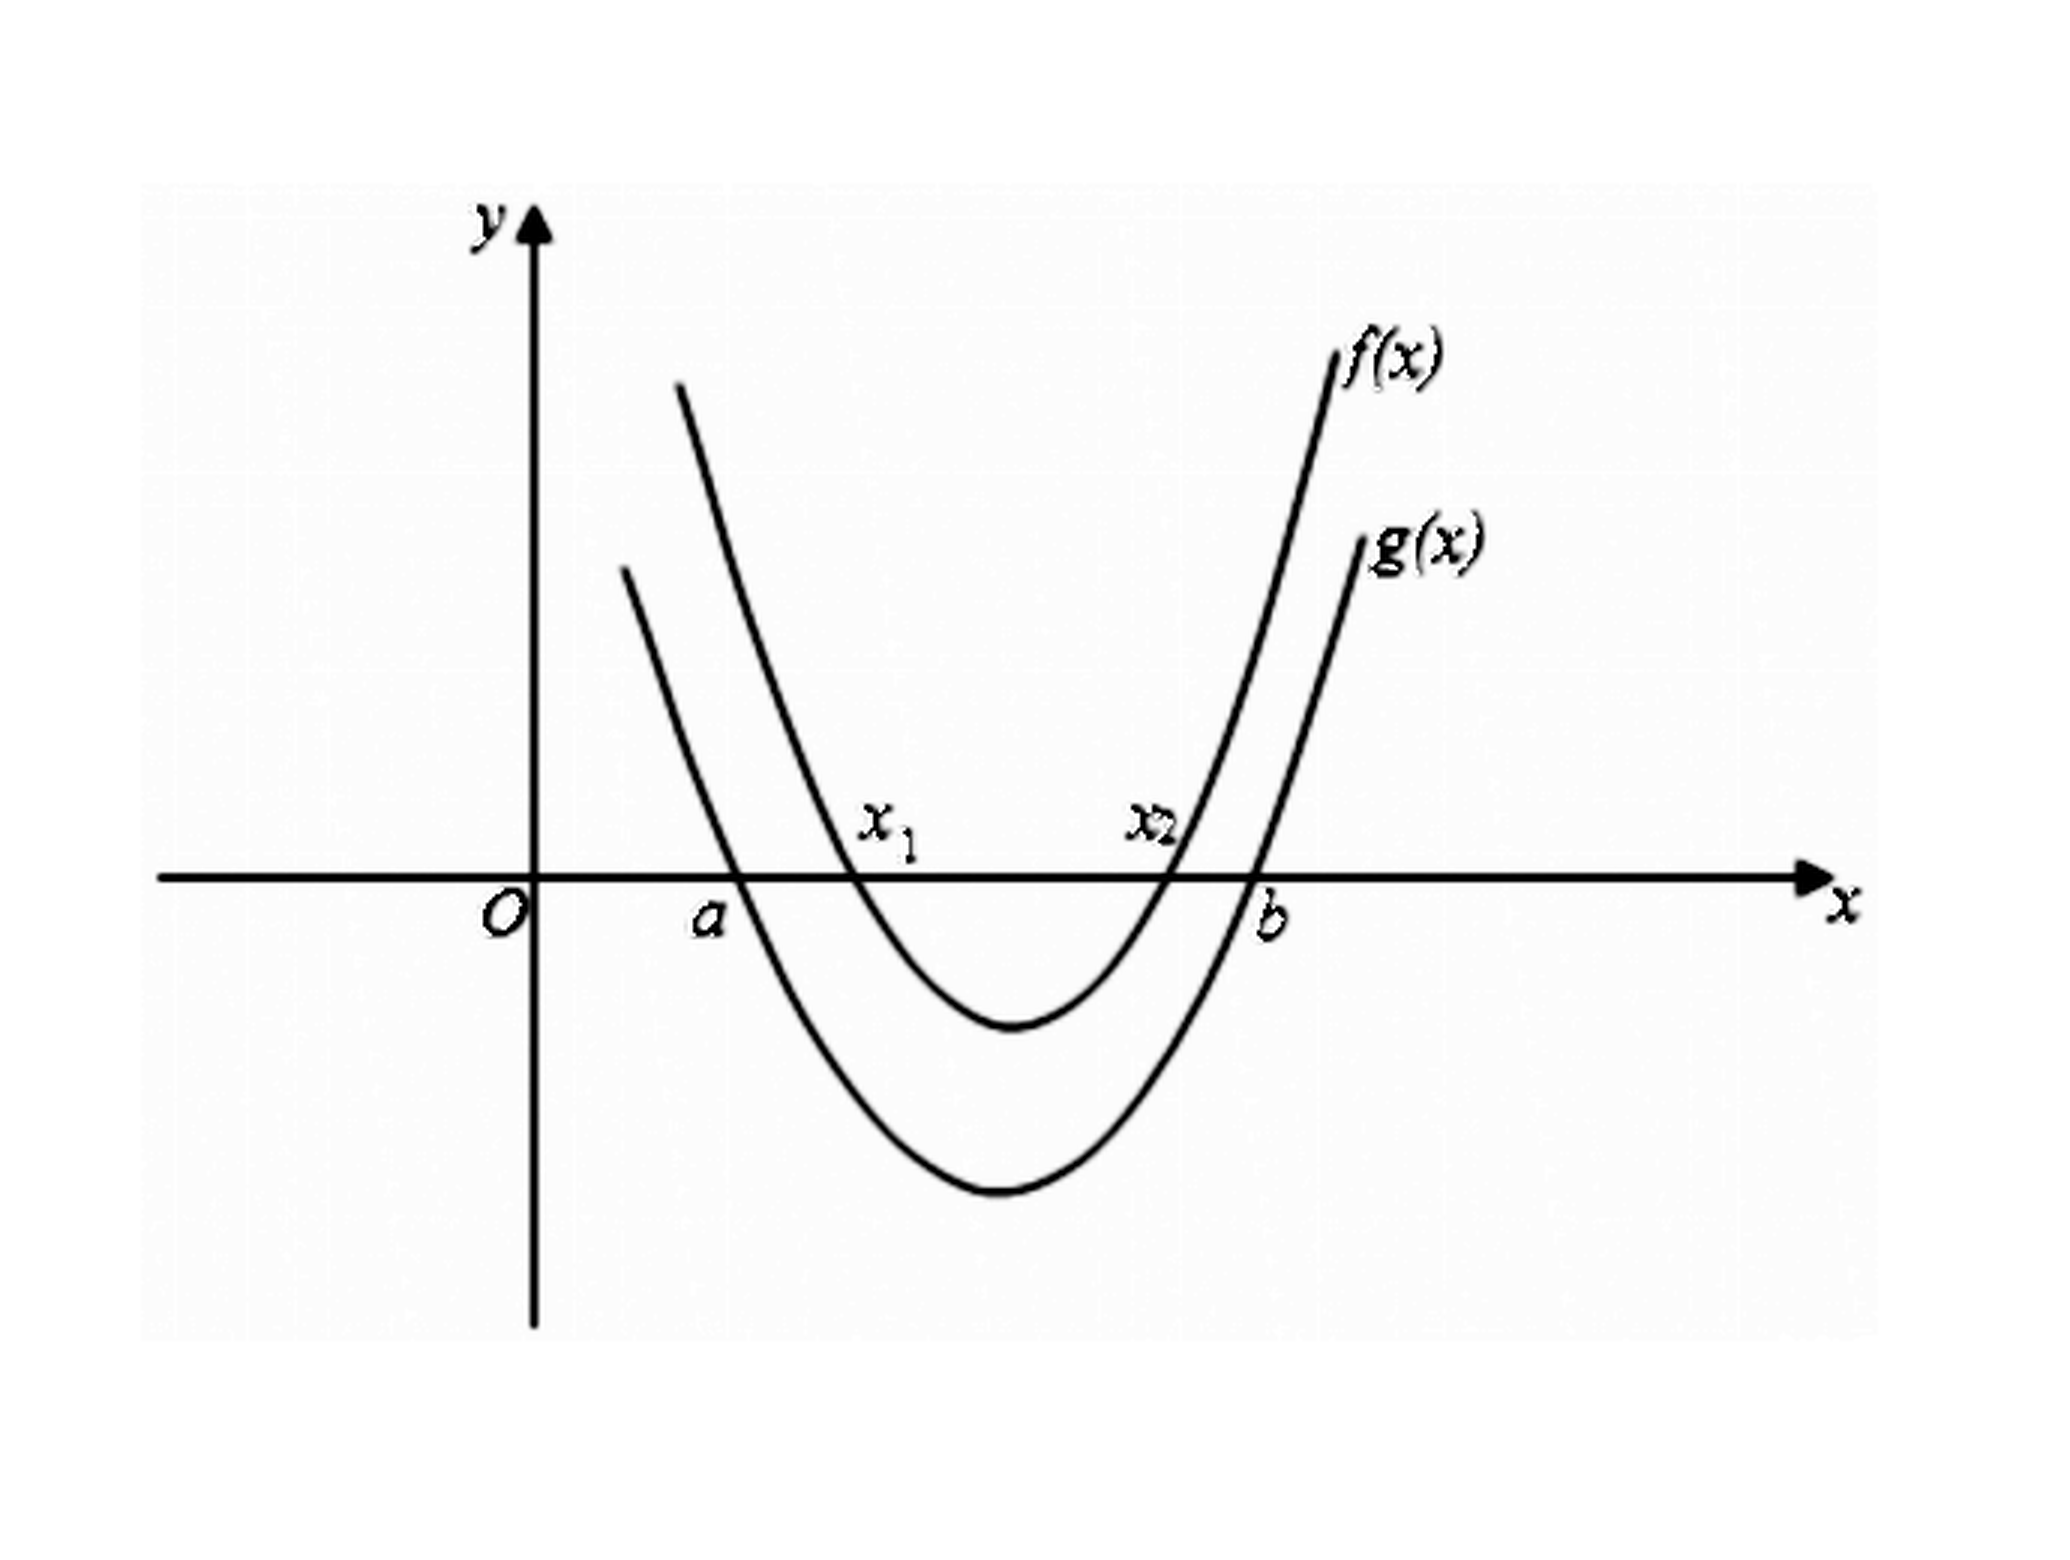
\includegraphics[width=0.52\textwidth]{figures/gao157_q16.png}
\end{center}

\step{由图像得 $a<x_1<x_2<b$，故选 $A$.}
\solend
\fi

\end{enumerate}

\bigsec{三、解答题}

\begin{enumerate}
\setcounter{enumi}{16}

% === Q17 === 解析 6 行；\overline{A}、\varnothing、\subseteq 无、cases
\item 设全集为 $\R$，$m\in\R$，集合 $A=\{x\mid 2<x<5\}$，$B=\{x\mid 2m\leqslant x\leqslant 5m-3\}$.

(1) 若 $m=2$，求 $\overline{A}\cup B$；

(2) 若 $A\cap B=B$，求 $m$ 的取值范围.

\ifanswer
\solbegin
\step{(1) $\overline{A}=\{x\mid x\leqslant2$ 或 $x\geqslant5\}$，当 $m=2$ 时，$B=\{x\mid 4\leqslant x\leqslant7\}$，}
\step{则 $\overline{A}\cup B=\{x\mid x\leqslant2$ 或 $x\geqslant4\}$；}
\step{(2) 因为 $A\cap B=B$，所以 $B$ 是 $A$ 的子集，}
\step{当 $B=\varnothing$ 时，$2m>5m-3$，解得 $m<1$；}
\step{当 $B\ne\varnothing$ 时，$\begin{cases}2m\leqslant5m-3\\2m>2\\5m-3<5\end{cases}$，解得 $1<m<\dfrac85$；}
\step{综上，$m$ 的取值范围是 $(-\infty,1)\cup\left(1,\dfrac85\right)$.}
\solend
\fi

% === Q18 === 解析 2 行；指数式、\lg、换底
\item (1) 设 $a^{2x}=3$，且 $a>0$，求 $\dfrac{a^{3x}+a^{-3x}}{a^x+a^{-x}}$ 的值；

(2) 已知 $\lg2=a, 10^b=3$，用 $a$ 及 $b$ 表示 $\log_{12}25$.

\ifanswer
\solbegin
\step{(1) $\dfrac{a^{3x}+a^{-3x}}{a^x+a^{-x}}=a^{2x}-1+a^{-2x}=3-1+\dfrac13=\dfrac73$；}
\step{(2) $\log_{12}25=\dfrac{\lg25}{\lg12}=\dfrac{2-2\lg2}{2\lg2+\lg3}=\dfrac{2-2a}{2a+b}$.}
\solend
\fi

% === Q19 === 解析 11 行；幂函数、$=0$ 笔误照录、\Delta、\sqrt5、cases
\item 已知幂函数 $f(x)=(m^2+m-1)x^{-2m^2+m+3}$ 在 $(0,+\infty)$ 上为严格增函数.

(1) 求 $f(x)$ 的解析式；

(2) 若 $k+kf(x)>f(x)-x-1$ 对任意实数 $x$ 都成立，求实数 $k$ 的取值范围；

(3) 若关于 $x$ 的不等式 $f(x)\leqslant8x-a$ 的解集中有且仅有 $5$ 个整数，求实数 $a$ 的范围.

\ifanswer
\solbegin
\step{(1) 由题意得 $m^2+m-1=1$，且 $-2m^2+m+3>0$，}
\step{解得 $m=-2$（舍去）或 $m=1$，所以 $f(x)=x^2$；}
\step{(2) $k+kf(x)>f(x)-x-1$ 可化为 $(k-1)x^2+x+k+1=0$ 恒成立，}
\step{当 $k=1$ 时，$x+2>0$，显然不恒成立；}
\step{当 $k\ne1$ 时，要使该二次不等式恒成立，只需 $\begin{cases}k-1>0\\[2pt]\Delta=1-4(k+1)(k-1)\leqslant0\end{cases}$，}
\step{解得 $k\geqslant\dfrac{\sqrt5}{2}$，即所求 $k$ 的范围是 $\left[\dfrac{\sqrt5}{2},+\infty\right)$；}
\step{(3) 不等式 $f(x)\leqslant8x-a$，即 $x^2-8x+a\leqslant0$ 有五个整数解，}
\step{令 $g(x)=x^2-8x+a$，因为该函数开口向上，对称轴为 $x=4$，}
\step{所以解集内的整数为 $2$，$3$，$4$，$5$，$6$，}
\step{由二次函数的性质得，只需 $\begin{cases}g(1)=1-8+a>0\\g(2)=4-8\times2+a\leqslant0\end{cases}$，解得 $7<a\leqslant12$，}
\step{故 $a$ 的取值范围是 $(7,12]$.}
\solend
\fi

% === Q20 === 解析 12 行；材料题、$a+b=1$、大根号、"因出"笔误、分母套分数
\item 问题：正数 $a$、$b$ 满足 $a+b=1$，求 $\dfrac1a+\dfrac2b$ 的最小值.

其中一种解法是：$\dfrac1a+\dfrac2b=\left(\dfrac1a+\dfrac2b\right)(a+b)=1+\dfrac ba+\dfrac{2a}{b}+2\geqslant3+2\sqrt2$，

当且仅当 $\dfrac ba=\dfrac{2a}{b}$ 且 $a+b=1$ 时，即 $a=\sqrt2-1$ 且 $b=2-\sqrt2$ 时取等号.

学习上述解法并解决下列问题：

(1) 若正实数 $x$、$y$ 满足 $x+y=1$，求 $\dfrac2x+\dfrac1y$ 的最小值；

(2) 若实数 $a$、$b$、$x$、$y$ 满足 $\dfrac{x^2}{a^2}-\dfrac{y^2}{b^2}=1$，求证：$a^2-b^2\leqslant(x-y)^2$；

(3) 利用 (2) 的结论，求代数式 $M=\sqrt{2m-5}-\sqrt{m-3}$ 的最小值，并求出使得 $M$ 最小的 $m$ 的值.

\ifanswer
\solbegin
\step{(1) $\dfrac2x+\dfrac1y=(x+y)\left(\dfrac2x+\dfrac1y\right)=3+\dfrac xy+\dfrac{2y}{x}\geqslant3+2\sqrt2$，}
\step{当且仅当 $\dfrac xy=\dfrac{2y}{x}$ 且 $x+y=1$ 时取等号；}
\step{(2) $a^2-b^2=(a^2-b^2)\left(\dfrac{x^2}{a^2}-\dfrac{y^2}{b^2}\right)=x^2+y^2-\left(\dfrac{a^2x^2}{b^2}+\dfrac{b^2y^2}{a^2}\right)$}
\step{$\leqslant x^2+y^2-2\sqrt{\dfrac{a^2x^2}{b^2}\cdot\dfrac{b^2y^2}{a^2}}=x^2+y^2-2xy=(x-y)^2$，}
\step{故当 $b^4x^2=a^4y^2$ 时，等号成立.}
\step{(3) 令 $x=\sqrt{2m-5}, y=\sqrt{m-3}$，由 $\begin{cases}2m-5\geqslant0\\m-3\geqslant0\end{cases}$ 得 $m\geqslant3$，}
\step{$x^2-y^2=(2m-5)-(m-3)=m-2>0$，}
\step{又 $x>0, y>0$，所以 $x>y$，所以 $\dfrac{x^2}{a^2}-\dfrac{y^2}{b^2}=1$，}
\step{由 $x^2-2y^2=1$，得 $\dfrac{x^2}{1}-\dfrac{y^2}{\frac12}=1$，因出 $a^2=1, b^2=\dfrac12$，}
\step{由 (2) 得 $M=\sqrt{2m-5}-\sqrt{m-3}=x-y\geqslant\sqrt{a^2-b^2}=\sqrt{1-\dfrac12}=\dfrac{\sqrt2}{2}$，}
\step{当且仅当 $\dfrac xy=\left(\dfrac ab\right)^2=2$ 取等号，结合 $x^2-2y^2=1$，解得 $x=\sqrt2, y=\dfrac{\sqrt2}{2}$，}
\step{即 $\sqrt{2m-5}=\sqrt2$，得 $m=\dfrac72$，所以 $m=\dfrac72$ 时，$M$ 取得最小值 $\dfrac{\sqrt2}{2}$.}
\solend
\fi

\end{enumerate}

\end{document}
"
% 紧凑版：xelatex "\def\iscompact{1}% 高一157_大境中学_期中.tex
%   —— 高一上数学"2026-2027 年大境中学高一上期中"（试卷版/答案版/紧凑版）
% 试卷版：xelatex 高一157_大境中学_期中.tex
% 答案版：xelatex "\def\isanswer{1}% 高一157_大境中学_期中.tex
%   —— 高一上数学"2026-2027 年大境中学高一上期中"（试卷版/答案版/紧凑版）
% 试卷版：xelatex 高一157_大境中学_期中.tex
% 答案版：xelatex "\def\isanswer{1}% 高一157_大境中学_期中.tex
%   —— 高一上数学"2026-2027 年大境中学高一上期中"（试卷版/答案版/紧凑版）
% 试卷版：xelatex 高一157_大境中学_期中.tex
% 答案版：xelatex "\def\isanswer{1}\input{高一157_大境中学_期中.tex}"
% 紧凑版：xelatex "\def\iscompact{1}\input{高一157_大境中学_期中.tex}"
%
% ① 原始材料：微信公众号"魔都数学加油站"文章，连载"27学年高一157"，原文标题
% "27学年高一157——2026-2027年上海市大境中学高一上期中"；
% 原文链接：https://mp.weixin.qq.com/s/s6eDMDVkxc2fcBe8LNm-Tw 。
% 正文为 8 张 PNG 页（01/02/03/04/06 为 4762×6735，05/07/08 为 2560×3620，
% 同一篇各页分辨率混排，逐页按各自分辨率裁图核对）。
% 体例：讲评版——填空 3—12（10 题）、选择 13—16（4 题）、解答 17—20（4 题），
% 共 18 题，自第 3 题起编（1、2 未印在本篇）；末题是第 20 题（不是 21）。
% 除第 4 题只印【答案】外，其余 17 题逐题印【解析】（逐题核实，见 ②）。
% 题目、答案、解析均据原图转录；卷面粉红色水印"魔都数学加油站"及公众号
% 页脚未录入。
% 全卷仅 1 幅配图：第 16 题解析内函数图像（"设 g(x)=(x-a)(x-b)，
% f(x)=g(x)+1，画出函数 g(x) 与函数 f(x) 的图像，如图所示"），
% 解析内配图仅答案版出，裁 figures/gao157_q16.png；逐页通读 8 页确认
% 无题目配图、无表格；08 页下半仅水印、无正文。
%
% 卷首标题：原卷印作"2026-2027 年大境中学高一上期中"，年份区间按全稿惯例排 en dash；
% 原卷卷面未印副标题，本稿按同期中卷知识模块口径补出"集合与常用逻辑用语、不等式、函数"。
%
% ② 与原卷的排版差异：
%   ① 原文从第 3 题起，本稿保留原题号；共 18 题三节，解答题 4 题到 20；
%      三节各自 \begin{enumerate}…\end{enumerate} + \setcounter{enumi}{2/12/16}
%      （题目溯源.py 按 \bigsec 切节、每节独立计 depth，只收 depth==1 的 \item，
%       见 高一156 头注②的订正）；
%   ② 第 4 题只印【答案】、无【解析】，提 \ans{}；其余 17 题逐题印【解析】、
%      逐题设 \solbegin…\solend；四道选择题答案在解析末句"故选 D／D／C／A"
%      （逐个放大复核）、括号 \mbox{（\quad）} 留空；答案版【答案】/【解析】
%      标记数 = 18 = 全卷题数（1 个 \ans ＋ 17 个 \solbegin）；
%   ③ 原卷卷面未印副标题，本稿按知识模块口径补出；
%   ④ 原卷填空横线按全稿惯例排 \blankline[4.4em]；选择题选项段前按惯例各加
%      \keepwithprev；解答题不留作答区、不加 \anspace（原卷为讲评版，109—113 起
%      全稿不用 \anspace）；
%   ⑤ 数集：Q4"$x、y\in R$"、Q6"$x\in R$"、Q10"$a\in Z$"、Q12"$n\in Z$"
%      "$n_1、n_2\in Z$"、Q17"全集为 R／$m\in R$"原卷印斜体 R/Z，按全稿惯例
%      归一 \R／\Z（参见 高一14 头注④、高一150 头注②⑤、高一153 头注⑤）；
%      绝对值排 \lvert…\rvert（Q6 $\lvert x-1\rvert$／$\lvert x+3\rvert$／
%      $\lvert 2x+2\rvert$），集合描述竖线排 \mid（Q12、Q17），空集 \varnothing
%      （Q17"$B=\varnothing$"），补集照原卷上划线排 \overline{A}（Q17），
%      不等号按全稿惯例排 \leqslant／\geqslant；
%   ⑥ 判别式三处（Q8"$\Delta=(-2m)^2-4(m+2)$"、Q15"$\Delta=(a+2)^2+4(a^2-4)<0$"、
%      Q19"$\Delta=1-4(k+1)(k-1)\leqslant0$"）放大比对同形、均为等腰偏高且右斜边
%      加粗的 \Delta，统一照录 \Delta；本卷无扁三角 \triangle 用例（与 高一142／
%      高一151／高一152 的 Δ/△ 混用卷不同）；
%   ⑦ "图像／图象"逐处照录不统一：Q9"图像过点 $(4,2)$""它的图像过点"、
%      Q16"画出函数 $g(x)$ 与函数 $f(x)$ 的图像""由图像得"用"图像"；
%      Q14 题干及解析四处均用"图象"（"的图象关于原点对称""图象关于 $y$ 轴对称"）；
%   ⑧ 原卷笔误／未化简式照录：
%      · Q5 解析"$2\sqrt4+1=5$"根号 4 原卷未化简，照录 \sqrt4；
%      · Q7 解析"$\lg\frac{E_1}{E_2}=\frac25\cdot(m_2-m_1)=\frac25(-1.45+26.7)=10.1$"
%        第一处有 \cdot、第二处无，逐处照录；题干"$m_1-m_2=-\frac52\lg\frac{E_1}{E_2}$"；
%      · Q10 解析"$f(1)=\frac{a+1}{1+2}\geqslant0$"与 cases 第二行分母均印 $1+2$、
%        未化简成 $3$，照录；
%      · Q19 (2)"可化为 $(k-1)x^2+x+k+1=0$ 恒成立"原卷印 $=0$（与 >0 恒成立
%        的题意不符），照录笔误；
%      · Q20 (3)"因出 $a^2=1, b^2=\frac12$"原卷印"因出"（当作"因此"），照录；
%      · Q20 (3)"得 $\frac{x^2}{1}-\frac{y^2}{\frac12}=1$"分母套分数、照录；
%   ⑨ 圈数字①②在文本模式（Q15 解析"①当 $a^2-4=0$ 时""②当 $a^2-4\ne0$ 时"，
%      共 2 枚）；子题标号 (1)(2)(3) 半角括号照录；行末西文句点 ASCII `.`；
%      行中全角逗号／顿号照录；半角逗号在数学组之间是全稿惯例、非笔误
%      （Q8"$x_1+x_2=2m, x_1x_2=m+2$"、Q12"$n\in Z$"、Q18"$\lg2=a, 10^b=3$"、
%      Q20"$a^2=1, b^2=\frac12$"等）；中文弯引号""照录（Q4 命题）；
%   ⑩ 自定义名词：Q11"交叉数"、Q12"$a\otimes b$"新定义运算、Q20"问题／
%      其中一种解法是／学习上述解法并解决下列问题"材料题，均照原卷录入；
%   ⑪ 配图：全卷 1 幅（逐页通读 8 页确认）——Q16 解析内函数图像（05 页右侧，
%      $f(x)$ 与 $g(x)$ 两条抛物线、标注 $a,x_1,x_2,b$），仅答案版出，
%      裁 figures/gao157_q16.png，去粉色水印、去色、3× LANCZOS 放大；
%      图放 \ifanswer 内 \solbegin…\solend 的两 \step 之间（高一108 第 6 题／
%      高一156 Q15 成例）；Q16 题干无"如图"、不需题目配图守卫。
%
% ③ 行数复核：一条 \step = 原卷解析的一个印刷行，cases 块作一个印刷行计；
%    跨半页重叠行（Q5 的"【解析】x-1>0…"、Q10 的"所以 a=-1 或 a=0"、
%    Q12 的"【解析】由 u⊗v…"、Q14 的"f(x)=x² 图象关于 y 轴对称"、
%    Q19 的"(1) 由题意得…"、Q20 的"(3) 令 x=…"等 hi_1/hi_2 两半页共有的行）
%    只计一次，别把原卷折行并起来。
%    逐题数（主会话逐页核对定稿）：Q3：1；Q4：0（只印【答案】、提 \ans{}，
%    不计入 \step 账）；Q5：2；Q6：5；Q7：2；Q8：5；Q9：3；Q10：4；
%    Q11：3；Q12：6；Q13：3；Q14：5；Q15：9；Q16：4；Q17：6；Q18：2；
%    Q19：11；Q20：12。合计 83 条 \step（本卷无 \stepm），与原卷逐题印刷行相等。
%    全卷 18 题：1 题只印【答案】（\ans）、17 题印【解析】（\solbegin…\solend），
%    答案版【答案】/【解析】标记数 = 18 = 全卷题数。
%    全卷除此 6 类外未发现其它笔误／自相矛盾处；17 题印【解析】、1 题印【答案】。
%
\documentclass[a4paper,11pt]{article}
\usepackage{common}

\begin{document}

\examtitlest[3]{2026--2027 年大境中学高一上期中}{集合与常用逻辑用语、不等式、函数}

\bigsec{一、填空题}

\begin{enumerate}
\setcounter{enumi}{2}

% === Q3 === 解析 1 行；$a,b$ 半角逗号照录
\item 若 $a=x^2-2x+1$，$b=x-3$，则 $a,b$ 的大小关系为\blankline[4.4em].

\ifanswer
\solbegin
\step{$a-b=x^2-3x+4=\left(x-\dfrac32\right)^2+\dfrac74>0$，所以 $a>b$.}
\solend
\fi

% === Q4 === 只印【答案】、无【解析】；中文弯引号、\R、顿号；提 \ans{}
\item 用反证法证明命题：“设 $x$、$y\in\R$. 若 $x+y>2$，则 $x>1$ 或 $y>1$”时，假设的内容应该是\blankline[4.4em].

\ifanswer
\ans{$x\leqslant1$ 且 $y\leqslant1$}
\fi

% === Q5 === 解析 2 行；$2\sqrt4+1=5$ 根号 4 未化简照录
\item 当 $x>1$ 时，$x+\dfrac4{x-1}$ 的最小值为\blankline[4.4em].

\ifanswer
\solbegin
\step{$x-1>0$，$x+\dfrac4{x-1}=(x-1)+\dfrac4{x-1}+1\geqslant2\sqrt4+1=5$，}
\step{当且仅当 $x-1=\dfrac4{x-1}$，即 $x=3$ 时取等号，故最小值为 $5$.}
\solend
\fi

% === Q6 === 解析 5 行；绝对值 \lvert…\rvert、\cup、\R
\item 设 $x\in\R$，方程 $\lvert x-1\rvert+\lvert x+3\rvert=\lvert 2x+2\rvert$ 的解集是\blankline[4.4em].

\ifanswer
\solbegin
\step{当 $x\leqslant-3$ 时，方程为 $1-x-x-3=-2x-2$，等式成立；}
\step{当 $-3<x\leqslant-1$ 时，方程为 $1-x+x+3=-2x-2$，解得 $x=-3$，舍去；}
\step{当 $-1<x<1$ 时，方程为 $1-x+x+3=2x+2$，解得 $x=1$，舍去；}
\step{当 $x\geqslant1$ 时，方程为 $x-1+x+3=2x+2$，等式成立，}
\step{综上，方程 $\lvert x-1\rvert+\lvert x+3\rvert=\lvert 2x+2\rvert$ 的解集为 $(-\infty,-3]\cup[1,+\infty)$.}
\solend
\fi

% === Q7 === 解析 2 行；星等材料题、\lg、\cdot 逐处照录、天狼星
\item 在天文学中，天体的明暗程度可以用星等或亮度来描述，两颗星的星等与亮度满足 $m_1-m_2=-\dfrac52\lg\dfrac{E_1}{E_2}$，其中星等为 $m_k$ 的星的亮度为 $E_k(k=1,2)$. 已知太阳的星等为 $-26.7$，天狼星的星等为 $-1.45$，则太阳与天狼星的亮度的比值为\blankline[4.4em].

\ifanswer
\solbegin
\step{两颗星的星等与亮度满足 $m_1-m_2=-\dfrac52\lg\dfrac{E_1}{E_2}$，令 $m_2=-1.45$，$m_1=-26.7$，}
\step{$\lg\dfrac{E_1}{E_2}=\dfrac25\cdot(m_2-m_1)=\dfrac25(-1.45+26.7)=10.1$，$\dfrac{E_1}{E_2}=10^{10.1}$.}
\solend
\fi

% === Q8 === 解析 5 行；韦达定理、判别式 \Delta、半角逗号在数学组间
\item 已知方程 $x^2-2mx+m+2=0$ 有两个实数根 $x_1,x_2$，满足 $x_1^2+x_2^2=2$，则实数 $m$ 的值为\blankline[4.4em].

\ifanswer
\solbegin
\step{对于方程 $x^2-2mx+m+2=0$，由韦达定理得 $x_1+x_2=2m, x_1x_2=m+2$，}
\step{又 $x_1^2+x_2^2=(x_1+x_2)^2-2x_1x_2=(2m)^2-2(m+2)=4m^2-2m-4=2$，}
\step{解得 $m=\dfrac32$ 或 $m=-1$，}
\step{因为方程有两个实数根，所以 $\Delta=(-2m)^2-4(m+2)=4m^2-4m-8\geqslant0$，}
\step{解得 $m\leqslant-1$ 或 $m\geqslant2$，故 $m=-1$.}
\solend
\fi

% === Q9 === 解析 3 行；"图像"照录、$x^\alpha$、$x^{1/2}=\sqrt{x}$
\item 已知幂函数 $y=f(x)$ 的图像过点 $(4,2)$，则不等式 $f(x^2-2x)<f(2-x)$ 的解集为\blankline[4.4em].

\ifanswer
\solbegin
\step{设幂函数 $y=f(x)=x^\alpha$，它的图像过点 $(4,2)$，所以 $4^\alpha=2$，$\alpha=\dfrac12$，}
\step{故 $f(x)=x^{\frac12}=\sqrt{x}$，由不等式 $f(x^2-2x)<f(2-x)$，}
\step{得 $0\leqslant x^2-2x<2-x$，得 $-1<x\leqslant0$，故解集为 $(-1,0]$.}
\solend
\fi

% === Q10 === 解析 4 行；$a\in\Z$、cases（分母 $1+2$ 未化简）、参数分离
\item 已知函数 $y=\dfrac{ax+1}{x+2}$（常数 $a\in\Z$）. 要使该函数在区间 $[1,+\infty)$ 上是严格减函数，并且函数值不恒为负，则满足条件的 $a$ 的取值为\blankline[4.4em].

\ifanswer
\solbegin
\step{函数参数分离为 $y=\dfrac{a(x+2)+1-2a}{x+2}=a+\dfrac{1-2a}{x+2}$，}
\step{若函数在区间 $[1,+\infty)$ 上严格减函数，则 $1-2a>0$，}
\step{且函数的最大值 $f(1)=\dfrac{a+1}{1+2}\geqslant0$，即 $\begin{cases}1-2a>0\\[2pt]\dfrac{a+1}{1+2}\geqslant0\end{cases}$，解得 $-1\leqslant a<\dfrac12$，又 $a\in\Z$，}
\step{所以 $a=-1$ 或 $a=0$.}
\solend
\fi

% === Q11 === 解析 3 行；"交叉数"自定义名词、$(-1)^t$、$2^5$、$32\times3=96$
\item 对非空集合 $A$ 中的每个元素 $t$，都乘以 $(-1)^t$ 再求和，称为集合 $A$ 的交叉数，例如 $A=\{2,3,6\}$，则集合 $A$ 的交叉数为 $(-1)^2\cdot2+(-1)^3\cdot3+(-1)^6\cdot6=5$. 若集合 $W=\{1,2,3,4,5,6\}$，则 $W$ 的所有非空子集的交叉数的总和为\blankline[4.4em].

\ifanswer
\solbegin
\step{固定 $W$ 中的任一元素，其余 $5$ 个元素各有选或不选两种情况，}
\step{因此该元素出现在 $2^5$ 个非空子集中，}
\step{所有交叉数的总和为 $2^5(-1+2-3+4-5+6)=32\times3=96$.}
\solend
\fi

% === Q12 === 解析 6 行；\otimes、\lambda、\mid、\Z、\times 与 \cdot 逐处照录
\item 对于任意两个正实数 $a$、$b$，定义 $a\otimes b=\lambda\cdot\dfrac ab$，其中常数 $\lambda\in\left(\dfrac{\sqrt2}{2},1\right)$. 若 $u\geqslant v>0$，且 $u\otimes v$ 与 $v\otimes u$ 都是集合 $\left\{x\mid x=\dfrac n2,n\in\Z\right\}$ 的元素，则 $u\otimes v=$\blankline[4.4em].

\ifanswer
\solbegin
\step{由 $u\otimes v$ 与 $v\otimes u$ 都是集合 $\left\{x\mid x=\dfrac n2,n\in\Z\right\}$ 的元素，}
\step{不妨设 $\lambda\times\dfrac uv=\dfrac12 n_1$，$\lambda\times\dfrac vu=\dfrac12 n_2$，$n_1$、$n_2\in\Z$，}
\step{因为 $u\geqslant v>0$，所以 $0<\dfrac vu\leqslant1$，因为 $\lambda\in\left(\dfrac{\sqrt2}{2},1\right)$，所以 $\dfrac12 n_2=\lambda\cdot\dfrac vu\in(0,1)$，}
\step{因为 $n_2\in\Z$，所以 $n_2=1$，即 $\dfrac12=\dfrac{\lambda v}{u}$，所以 $\lambda=\dfrac{u}{2v}\in\left(\dfrac{\sqrt2}{2},1\right)$，}
\step{所以 $\dfrac uv\in(\sqrt2,2)$，$\dfrac{u^2}{v^2}\in(2,4)$，则 $\lambda\cdot\dfrac uv=\dfrac{u^2}{v^2}\times\dfrac12=\dfrac12 n_1\in(1,2)$，}
\step{因为 $n_1\in\Z$，所以 $n_1=3$，$\dfrac12 n_1=\dfrac32$，故 $u\otimes v=\dfrac32$.}
\solend
\fi

\end{enumerate}

\bigsec{二、选择题}

\begin{enumerate}
\setcounter{enumi}{12}

% === Q13 === 解析 3 行；选项段 \keepwithprev；故选 D
\item 下列不等式成立的为\mbox{（\quad）}

\keepwithprev
A. 若 $a>b$，则 $ac^2>bc^2$\qquad B. 若 $a>b$，则 $a^2>b^2$

C. 若 $a>b$，$c>d$，则 $a+b>c+d$\qquad D. 若 $a>b$，则 $a^3>b^3$

\ifanswer
\solbegin
\step{A 中 $c=0$ 时不成立；B 取 $a=1$，$b=-2$ 不成立；}
\step{C 取 $a=1$，$b=0$，$c=5$，$d=0$ 不成立.}
\step{幂函数 $y=x^3$ 在实数集上严格递增，所以 $a>b\Rightarrow a^3>b^3$，故选 $D$.}
\solend
\fi

% === Q14 === 解析 5 行；"图象"四处照录；故选 D
\item 幂函数 $f(x)=x^\alpha$ 的图象关于原点对称，且在 $(-\infty,0)$ 上是严格增函数，则 $f(x)$ 可以是\mbox{（\quad）}

\keepwithprev
A. $f(x)=x^{-1}$\qquad B. $f(x)=x^{\frac12}$\qquad C. $f(x)=x^2$\qquad D. $f(x)=x^3$

\ifanswer
\solbegin
\step{$f(x)=\dfrac1x$ 的图象关于原点对称，在 $(-\infty,0)$ 上是严格减函数，故 $A$ 错误；}
\step{$f(x)=x^{\frac12}$ 在 $(-\infty,0)$ 上无意义，故 $B$ 错误；}
\step{$f(x)=x^2$ 图象关于 $y$ 轴对称，故 $C$ 错误；}
\step{$f(x)=x^3$ 的图象关于原点对称，且在 $(-\infty,0)$ 上是严格增函数，故 $D$ 正确.}
\step{故选 $D$.}
\solend
\fi

% === Q15 === 解析 9 行；圈数字①②、\Delta、cases；故选 C
\item 若关于 $x$ 的不等式 $(a^2-4)x^2+(a+2)x-1\geqslant0$ 的解集不为空集，则实数 $a$ 的取值范围为\mbox{（\quad）}

\keepwithprev
A. $\left(-2,\dfrac65\right]$\qquad B. $\left[-2,\dfrac65\right]$

C. $(-\infty,-2)\cup\left[\dfrac65,+\infty\right)$\qquad D. $(-\infty,-2]\cup\left[\dfrac65,+\infty\right)$

\ifanswer
\solbegin
\step{①当 $a^2-4=0$ 时，$a=\pm2$，}
\step{若 $a=2$ 时，原不等式为 $4x-1\geqslant0$，则不等式的解集不是空集；}
\step{若 $a=-2$ 时，原不等式为 $-1\geqslant0$，无解，不符合题意；}
\step{②当 $a^2-4\ne0$ 时，$a\ne\pm2$，}
\step{若 $(a^2-4)x^2+(a+2)x-1\geqslant0$ 的解集是空集，则 $\begin{cases}a^2-4<0\\[2pt]\Delta=(a+2)^2+4(a^2-4)<0\end{cases}$，}
\step{解得 $-2<a<\dfrac65$，}
\step{则当不等式 $(a^2-4)x^2+(a+2)x-1\geqslant0$ 的解集不为空集时，}
\step{有 $a<-2$ 或 $a\geqslant\dfrac65$ 且 $a\ne2$，}
\step{综上，实数 $a$ 的取值范围为 $(-\infty,-2)\cup\left[\dfrac65,+\infty\right)$，故选 $C$.}
\solend
\fi

% === Q16 === 解析 4 行＋1 幅解析内配图（仅答案版）；"图像"照录；故选 A
\item 已知实数 $a<b$，关于 $x$ 的不等式 $x^2-(a+b)x+ab+1<0$ 的解集为 $(x_1,x_2)$，则实数 $a$、$b$、$x_1$、$x_2$ 从小到大的排列是\mbox{（\quad）}

\keepwithprev
A. $a<x_1<x_2<b$\qquad B. $x_1<a<b<x_2$\qquad C. $a<x_1<b<x_2$\qquad D. $x_1<a<x_2<b$

\ifanswer
\solbegin
\step{不等式 $x^2-(a+b)x+ab+1<0$ 可化为 $(x-a)(x-b)+1<0$，}
\step{设 $g(x)=(x-a)(x-b)$，$f(x)=g(x)+1$，}
\step{画出函数 $g(x)$ 与函数 $f(x)$ 的图像，如图所示，}

\begin{center}
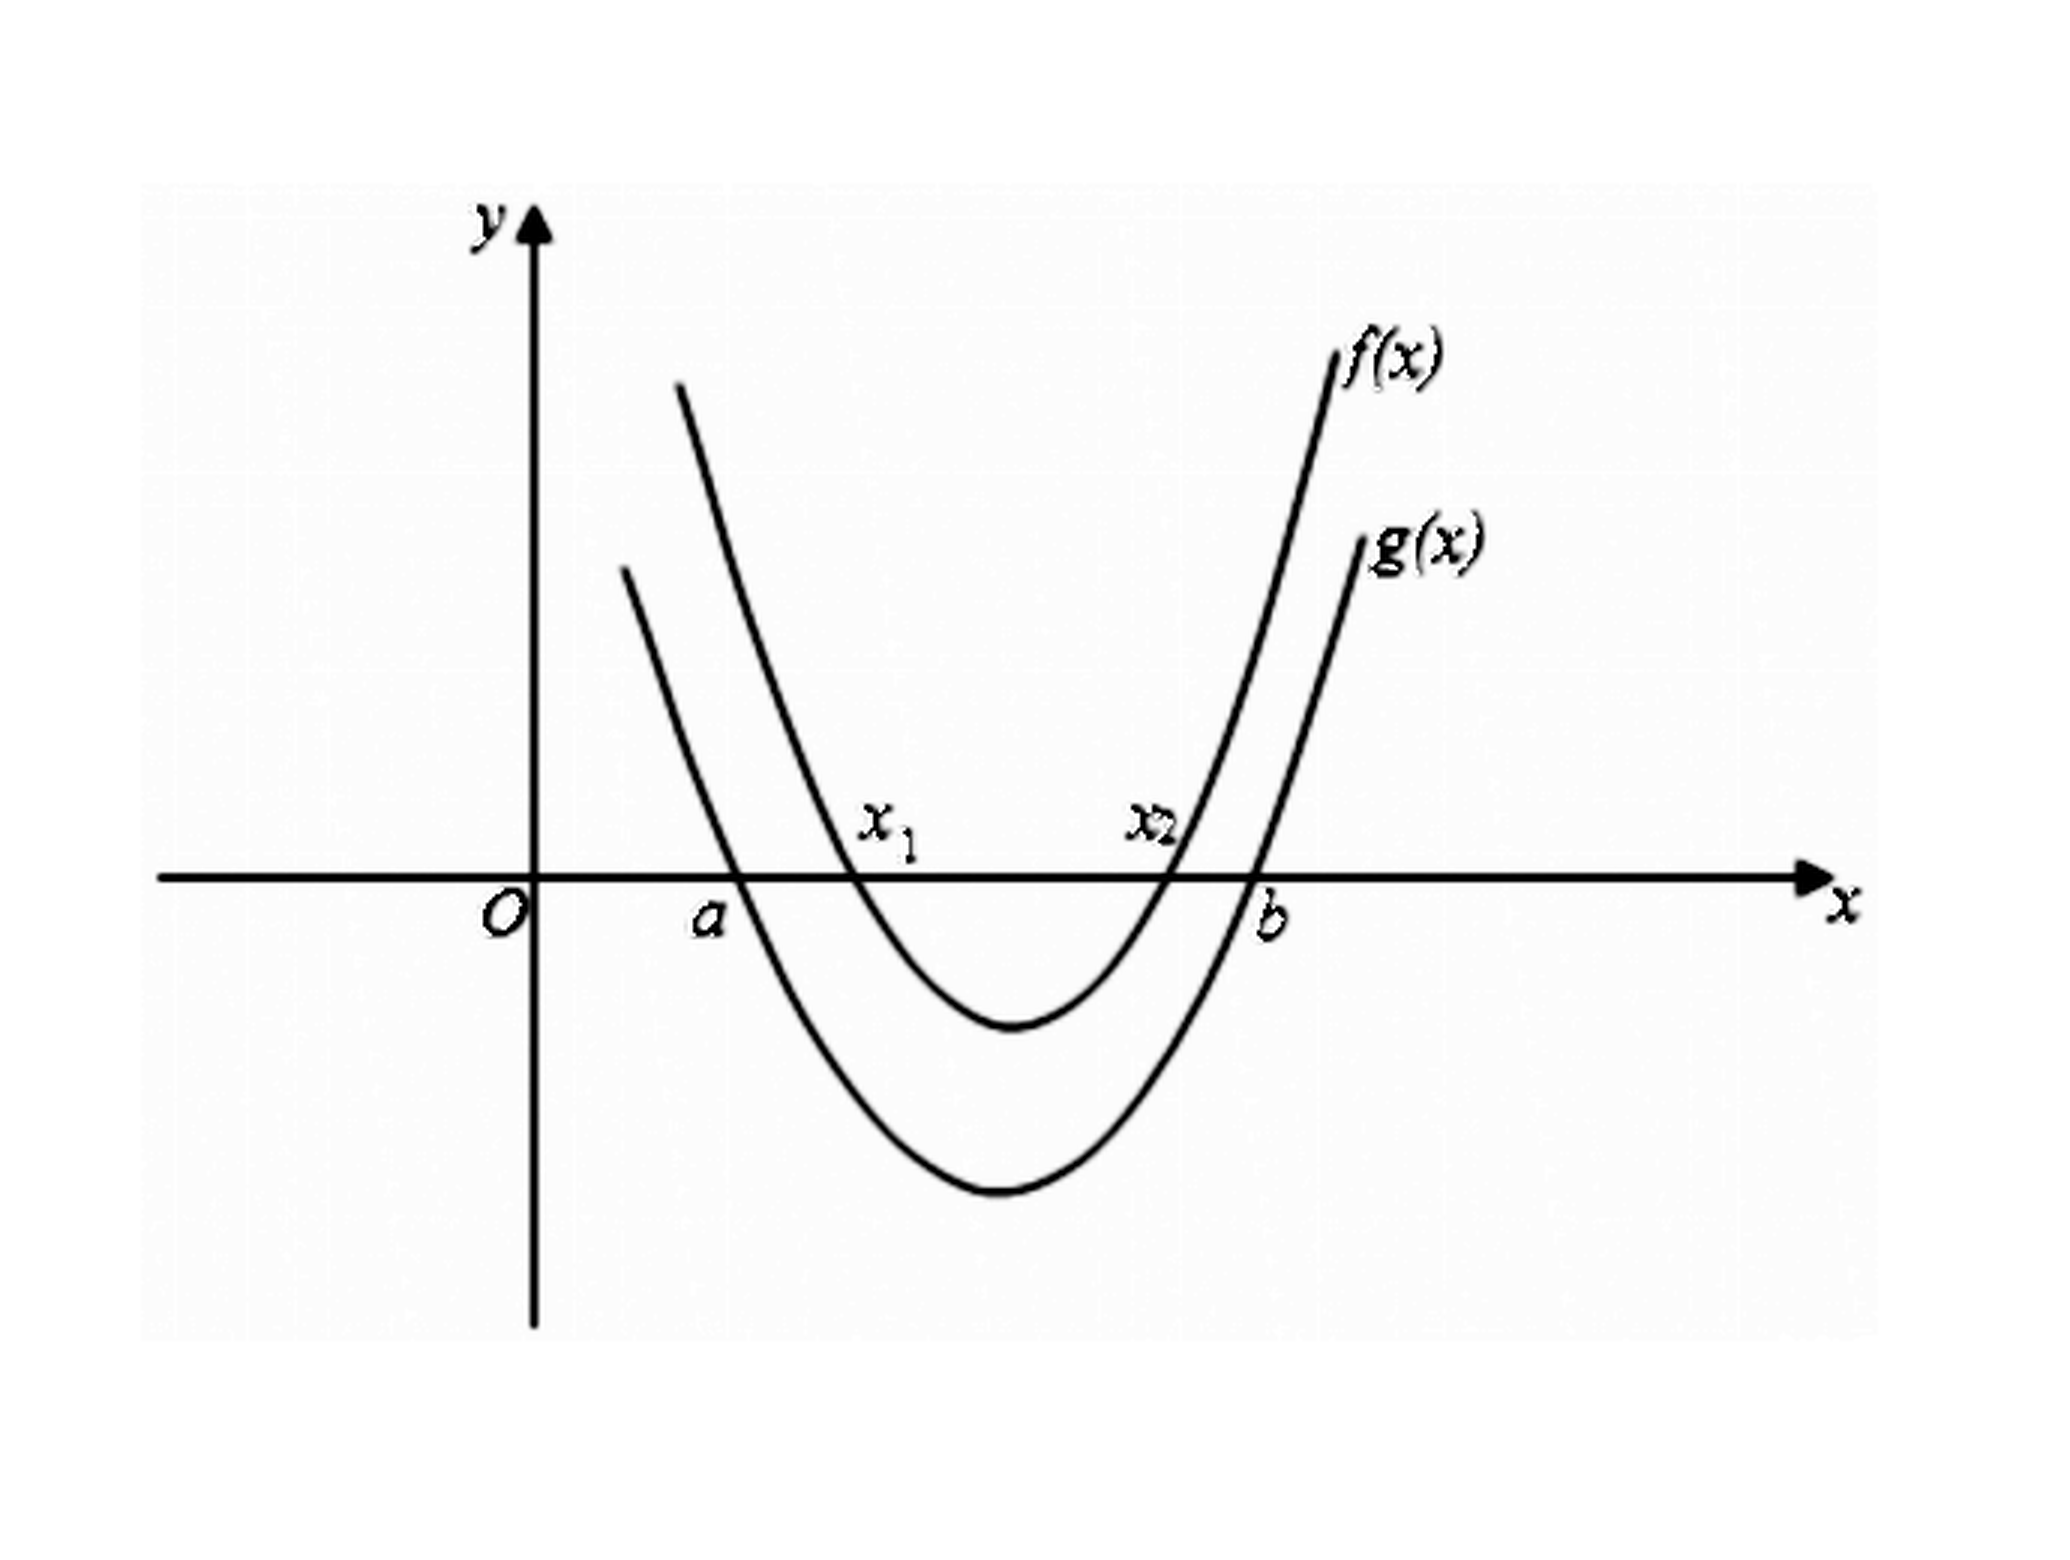
\includegraphics[width=0.52\textwidth]{figures/gao157_q16.png}
\end{center}

\step{由图像得 $a<x_1<x_2<b$，故选 $A$.}
\solend
\fi

\end{enumerate}

\bigsec{三、解答题}

\begin{enumerate}
\setcounter{enumi}{16}

% === Q17 === 解析 6 行；\overline{A}、\varnothing、\subseteq 无、cases
\item 设全集为 $\R$，$m\in\R$，集合 $A=\{x\mid 2<x<5\}$，$B=\{x\mid 2m\leqslant x\leqslant 5m-3\}$.

(1) 若 $m=2$，求 $\overline{A}\cup B$；

(2) 若 $A\cap B=B$，求 $m$ 的取值范围.

\ifanswer
\solbegin
\step{(1) $\overline{A}=\{x\mid x\leqslant2$ 或 $x\geqslant5\}$，当 $m=2$ 时，$B=\{x\mid 4\leqslant x\leqslant7\}$，}
\step{则 $\overline{A}\cup B=\{x\mid x\leqslant2$ 或 $x\geqslant4\}$；}
\step{(2) 因为 $A\cap B=B$，所以 $B$ 是 $A$ 的子集，}
\step{当 $B=\varnothing$ 时，$2m>5m-3$，解得 $m<1$；}
\step{当 $B\ne\varnothing$ 时，$\begin{cases}2m\leqslant5m-3\\2m>2\\5m-3<5\end{cases}$，解得 $1<m<\dfrac85$；}
\step{综上，$m$ 的取值范围是 $(-\infty,1)\cup\left(1,\dfrac85\right)$.}
\solend
\fi

% === Q18 === 解析 2 行；指数式、\lg、换底
\item (1) 设 $a^{2x}=3$，且 $a>0$，求 $\dfrac{a^{3x}+a^{-3x}}{a^x+a^{-x}}$ 的值；

(2) 已知 $\lg2=a, 10^b=3$，用 $a$ 及 $b$ 表示 $\log_{12}25$.

\ifanswer
\solbegin
\step{(1) $\dfrac{a^{3x}+a^{-3x}}{a^x+a^{-x}}=a^{2x}-1+a^{-2x}=3-1+\dfrac13=\dfrac73$；}
\step{(2) $\log_{12}25=\dfrac{\lg25}{\lg12}=\dfrac{2-2\lg2}{2\lg2+\lg3}=\dfrac{2-2a}{2a+b}$.}
\solend
\fi

% === Q19 === 解析 11 行；幂函数、$=0$ 笔误照录、\Delta、\sqrt5、cases
\item 已知幂函数 $f(x)=(m^2+m-1)x^{-2m^2+m+3}$ 在 $(0,+\infty)$ 上为严格增函数.

(1) 求 $f(x)$ 的解析式；

(2) 若 $k+kf(x)>f(x)-x-1$ 对任意实数 $x$ 都成立，求实数 $k$ 的取值范围；

(3) 若关于 $x$ 的不等式 $f(x)\leqslant8x-a$ 的解集中有且仅有 $5$ 个整数，求实数 $a$ 的范围.

\ifanswer
\solbegin
\step{(1) 由题意得 $m^2+m-1=1$，且 $-2m^2+m+3>0$，}
\step{解得 $m=-2$（舍去）或 $m=1$，所以 $f(x)=x^2$；}
\step{(2) $k+kf(x)>f(x)-x-1$ 可化为 $(k-1)x^2+x+k+1=0$ 恒成立，}
\step{当 $k=1$ 时，$x+2>0$，显然不恒成立；}
\step{当 $k\ne1$ 时，要使该二次不等式恒成立，只需 $\begin{cases}k-1>0\\[2pt]\Delta=1-4(k+1)(k-1)\leqslant0\end{cases}$，}
\step{解得 $k\geqslant\dfrac{\sqrt5}{2}$，即所求 $k$ 的范围是 $\left[\dfrac{\sqrt5}{2},+\infty\right)$；}
\step{(3) 不等式 $f(x)\leqslant8x-a$，即 $x^2-8x+a\leqslant0$ 有五个整数解，}
\step{令 $g(x)=x^2-8x+a$，因为该函数开口向上，对称轴为 $x=4$，}
\step{所以解集内的整数为 $2$，$3$，$4$，$5$，$6$，}
\step{由二次函数的性质得，只需 $\begin{cases}g(1)=1-8+a>0\\g(2)=4-8\times2+a\leqslant0\end{cases}$，解得 $7<a\leqslant12$，}
\step{故 $a$ 的取值范围是 $(7,12]$.}
\solend
\fi

% === Q20 === 解析 12 行；材料题、$a+b=1$、大根号、"因出"笔误、分母套分数
\item 问题：正数 $a$、$b$ 满足 $a+b=1$，求 $\dfrac1a+\dfrac2b$ 的最小值.

其中一种解法是：$\dfrac1a+\dfrac2b=\left(\dfrac1a+\dfrac2b\right)(a+b)=1+\dfrac ba+\dfrac{2a}{b}+2\geqslant3+2\sqrt2$，

当且仅当 $\dfrac ba=\dfrac{2a}{b}$ 且 $a+b=1$ 时，即 $a=\sqrt2-1$ 且 $b=2-\sqrt2$ 时取等号.

学习上述解法并解决下列问题：

(1) 若正实数 $x$、$y$ 满足 $x+y=1$，求 $\dfrac2x+\dfrac1y$ 的最小值；

(2) 若实数 $a$、$b$、$x$、$y$ 满足 $\dfrac{x^2}{a^2}-\dfrac{y^2}{b^2}=1$，求证：$a^2-b^2\leqslant(x-y)^2$；

(3) 利用 (2) 的结论，求代数式 $M=\sqrt{2m-5}-\sqrt{m-3}$ 的最小值，并求出使得 $M$ 最小的 $m$ 的值.

\ifanswer
\solbegin
\step{(1) $\dfrac2x+\dfrac1y=(x+y)\left(\dfrac2x+\dfrac1y\right)=3+\dfrac xy+\dfrac{2y}{x}\geqslant3+2\sqrt2$，}
\step{当且仅当 $\dfrac xy=\dfrac{2y}{x}$ 且 $x+y=1$ 时取等号；}
\step{(2) $a^2-b^2=(a^2-b^2)\left(\dfrac{x^2}{a^2}-\dfrac{y^2}{b^2}\right)=x^2+y^2-\left(\dfrac{a^2x^2}{b^2}+\dfrac{b^2y^2}{a^2}\right)$}
\step{$\leqslant x^2+y^2-2\sqrt{\dfrac{a^2x^2}{b^2}\cdot\dfrac{b^2y^2}{a^2}}=x^2+y^2-2xy=(x-y)^2$，}
\step{故当 $b^4x^2=a^4y^2$ 时，等号成立.}
\step{(3) 令 $x=\sqrt{2m-5}, y=\sqrt{m-3}$，由 $\begin{cases}2m-5\geqslant0\\m-3\geqslant0\end{cases}$ 得 $m\geqslant3$，}
\step{$x^2-y^2=(2m-5)-(m-3)=m-2>0$，}
\step{又 $x>0, y>0$，所以 $x>y$，所以 $\dfrac{x^2}{a^2}-\dfrac{y^2}{b^2}=1$，}
\step{由 $x^2-2y^2=1$，得 $\dfrac{x^2}{1}-\dfrac{y^2}{\frac12}=1$，因出 $a^2=1, b^2=\dfrac12$，}
\step{由 (2) 得 $M=\sqrt{2m-5}-\sqrt{m-3}=x-y\geqslant\sqrt{a^2-b^2}=\sqrt{1-\dfrac12}=\dfrac{\sqrt2}{2}$，}
\step{当且仅当 $\dfrac xy=\left(\dfrac ab\right)^2=2$ 取等号，结合 $x^2-2y^2=1$，解得 $x=\sqrt2, y=\dfrac{\sqrt2}{2}$，}
\step{即 $\sqrt{2m-5}=\sqrt2$，得 $m=\dfrac72$，所以 $m=\dfrac72$ 时，$M$ 取得最小值 $\dfrac{\sqrt2}{2}$.}
\solend
\fi

\end{enumerate}

\end{document}
"
% 紧凑版：xelatex "\def\iscompact{1}% 高一157_大境中学_期中.tex
%   —— 高一上数学"2026-2027 年大境中学高一上期中"（试卷版/答案版/紧凑版）
% 试卷版：xelatex 高一157_大境中学_期中.tex
% 答案版：xelatex "\def\isanswer{1}\input{高一157_大境中学_期中.tex}"
% 紧凑版：xelatex "\def\iscompact{1}\input{高一157_大境中学_期中.tex}"
%
% ① 原始材料：微信公众号"魔都数学加油站"文章，连载"27学年高一157"，原文标题
% "27学年高一157——2026-2027年上海市大境中学高一上期中"；
% 原文链接：https://mp.weixin.qq.com/s/s6eDMDVkxc2fcBe8LNm-Tw 。
% 正文为 8 张 PNG 页（01/02/03/04/06 为 4762×6735，05/07/08 为 2560×3620，
% 同一篇各页分辨率混排，逐页按各自分辨率裁图核对）。
% 体例：讲评版——填空 3—12（10 题）、选择 13—16（4 题）、解答 17—20（4 题），
% 共 18 题，自第 3 题起编（1、2 未印在本篇）；末题是第 20 题（不是 21）。
% 除第 4 题只印【答案】外，其余 17 题逐题印【解析】（逐题核实，见 ②）。
% 题目、答案、解析均据原图转录；卷面粉红色水印"魔都数学加油站"及公众号
% 页脚未录入。
% 全卷仅 1 幅配图：第 16 题解析内函数图像（"设 g(x)=(x-a)(x-b)，
% f(x)=g(x)+1，画出函数 g(x) 与函数 f(x) 的图像，如图所示"），
% 解析内配图仅答案版出，裁 figures/gao157_q16.png；逐页通读 8 页确认
% 无题目配图、无表格；08 页下半仅水印、无正文。
%
% 卷首标题：原卷印作"2026-2027 年大境中学高一上期中"，年份区间按全稿惯例排 en dash；
% 原卷卷面未印副标题，本稿按同期中卷知识模块口径补出"集合与常用逻辑用语、不等式、函数"。
%
% ② 与原卷的排版差异：
%   ① 原文从第 3 题起，本稿保留原题号；共 18 题三节，解答题 4 题到 20；
%      三节各自 \begin{enumerate}…\end{enumerate} + \setcounter{enumi}{2/12/16}
%      （题目溯源.py 按 \bigsec 切节、每节独立计 depth，只收 depth==1 的 \item，
%       见 高一156 头注②的订正）；
%   ② 第 4 题只印【答案】、无【解析】，提 \ans{}；其余 17 题逐题印【解析】、
%      逐题设 \solbegin…\solend；四道选择题答案在解析末句"故选 D／D／C／A"
%      （逐个放大复核）、括号 \mbox{（\quad）} 留空；答案版【答案】/【解析】
%      标记数 = 18 = 全卷题数（1 个 \ans ＋ 17 个 \solbegin）；
%   ③ 原卷卷面未印副标题，本稿按知识模块口径补出；
%   ④ 原卷填空横线按全稿惯例排 \blankline[4.4em]；选择题选项段前按惯例各加
%      \keepwithprev；解答题不留作答区、不加 \anspace（原卷为讲评版，109—113 起
%      全稿不用 \anspace）；
%   ⑤ 数集：Q4"$x、y\in R$"、Q6"$x\in R$"、Q10"$a\in Z$"、Q12"$n\in Z$"
%      "$n_1、n_2\in Z$"、Q17"全集为 R／$m\in R$"原卷印斜体 R/Z，按全稿惯例
%      归一 \R／\Z（参见 高一14 头注④、高一150 头注②⑤、高一153 头注⑤）；
%      绝对值排 \lvert…\rvert（Q6 $\lvert x-1\rvert$／$\lvert x+3\rvert$／
%      $\lvert 2x+2\rvert$），集合描述竖线排 \mid（Q12、Q17），空集 \varnothing
%      （Q17"$B=\varnothing$"），补集照原卷上划线排 \overline{A}（Q17），
%      不等号按全稿惯例排 \leqslant／\geqslant；
%   ⑥ 判别式三处（Q8"$\Delta=(-2m)^2-4(m+2)$"、Q15"$\Delta=(a+2)^2+4(a^2-4)<0$"、
%      Q19"$\Delta=1-4(k+1)(k-1)\leqslant0$"）放大比对同形、均为等腰偏高且右斜边
%      加粗的 \Delta，统一照录 \Delta；本卷无扁三角 \triangle 用例（与 高一142／
%      高一151／高一152 的 Δ/△ 混用卷不同）；
%   ⑦ "图像／图象"逐处照录不统一：Q9"图像过点 $(4,2)$""它的图像过点"、
%      Q16"画出函数 $g(x)$ 与函数 $f(x)$ 的图像""由图像得"用"图像"；
%      Q14 题干及解析四处均用"图象"（"的图象关于原点对称""图象关于 $y$ 轴对称"）；
%   ⑧ 原卷笔误／未化简式照录：
%      · Q5 解析"$2\sqrt4+1=5$"根号 4 原卷未化简，照录 \sqrt4；
%      · Q7 解析"$\lg\frac{E_1}{E_2}=\frac25\cdot(m_2-m_1)=\frac25(-1.45+26.7)=10.1$"
%        第一处有 \cdot、第二处无，逐处照录；题干"$m_1-m_2=-\frac52\lg\frac{E_1}{E_2}$"；
%      · Q10 解析"$f(1)=\frac{a+1}{1+2}\geqslant0$"与 cases 第二行分母均印 $1+2$、
%        未化简成 $3$，照录；
%      · Q19 (2)"可化为 $(k-1)x^2+x+k+1=0$ 恒成立"原卷印 $=0$（与 >0 恒成立
%        的题意不符），照录笔误；
%      · Q20 (3)"因出 $a^2=1, b^2=\frac12$"原卷印"因出"（当作"因此"），照录；
%      · Q20 (3)"得 $\frac{x^2}{1}-\frac{y^2}{\frac12}=1$"分母套分数、照录；
%   ⑨ 圈数字①②在文本模式（Q15 解析"①当 $a^2-4=0$ 时""②当 $a^2-4\ne0$ 时"，
%      共 2 枚）；子题标号 (1)(2)(3) 半角括号照录；行末西文句点 ASCII `.`；
%      行中全角逗号／顿号照录；半角逗号在数学组之间是全稿惯例、非笔误
%      （Q8"$x_1+x_2=2m, x_1x_2=m+2$"、Q12"$n\in Z$"、Q18"$\lg2=a, 10^b=3$"、
%      Q20"$a^2=1, b^2=\frac12$"等）；中文弯引号""照录（Q4 命题）；
%   ⑩ 自定义名词：Q11"交叉数"、Q12"$a\otimes b$"新定义运算、Q20"问题／
%      其中一种解法是／学习上述解法并解决下列问题"材料题，均照原卷录入；
%   ⑪ 配图：全卷 1 幅（逐页通读 8 页确认）——Q16 解析内函数图像（05 页右侧，
%      $f(x)$ 与 $g(x)$ 两条抛物线、标注 $a,x_1,x_2,b$），仅答案版出，
%      裁 figures/gao157_q16.png，去粉色水印、去色、3× LANCZOS 放大；
%      图放 \ifanswer 内 \solbegin…\solend 的两 \step 之间（高一108 第 6 题／
%      高一156 Q15 成例）；Q16 题干无"如图"、不需题目配图守卫。
%
% ③ 行数复核：一条 \step = 原卷解析的一个印刷行，cases 块作一个印刷行计；
%    跨半页重叠行（Q5 的"【解析】x-1>0…"、Q10 的"所以 a=-1 或 a=0"、
%    Q12 的"【解析】由 u⊗v…"、Q14 的"f(x)=x² 图象关于 y 轴对称"、
%    Q19 的"(1) 由题意得…"、Q20 的"(3) 令 x=…"等 hi_1/hi_2 两半页共有的行）
%    只计一次，别把原卷折行并起来。
%    逐题数（主会话逐页核对定稿）：Q3：1；Q4：0（只印【答案】、提 \ans{}，
%    不计入 \step 账）；Q5：2；Q6：5；Q7：2；Q8：5；Q9：3；Q10：4；
%    Q11：3；Q12：6；Q13：3；Q14：5；Q15：9；Q16：4；Q17：6；Q18：2；
%    Q19：11；Q20：12。合计 83 条 \step（本卷无 \stepm），与原卷逐题印刷行相等。
%    全卷 18 题：1 题只印【答案】（\ans）、17 题印【解析】（\solbegin…\solend），
%    答案版【答案】/【解析】标记数 = 18 = 全卷题数。
%    全卷除此 6 类外未发现其它笔误／自相矛盾处；17 题印【解析】、1 题印【答案】。
%
\documentclass[a4paper,11pt]{article}
\usepackage{common}

\begin{document}

\examtitlest[3]{2026--2027 年大境中学高一上期中}{集合与常用逻辑用语、不等式、函数}

\bigsec{一、填空题}

\begin{enumerate}
\setcounter{enumi}{2}

% === Q3 === 解析 1 行；$a,b$ 半角逗号照录
\item 若 $a=x^2-2x+1$，$b=x-3$，则 $a,b$ 的大小关系为\blankline[4.4em].

\ifanswer
\solbegin
\step{$a-b=x^2-3x+4=\left(x-\dfrac32\right)^2+\dfrac74>0$，所以 $a>b$.}
\solend
\fi

% === Q4 === 只印【答案】、无【解析】；中文弯引号、\R、顿号；提 \ans{}
\item 用反证法证明命题：“设 $x$、$y\in\R$. 若 $x+y>2$，则 $x>1$ 或 $y>1$”时，假设的内容应该是\blankline[4.4em].

\ifanswer
\ans{$x\leqslant1$ 且 $y\leqslant1$}
\fi

% === Q5 === 解析 2 行；$2\sqrt4+1=5$ 根号 4 未化简照录
\item 当 $x>1$ 时，$x+\dfrac4{x-1}$ 的最小值为\blankline[4.4em].

\ifanswer
\solbegin
\step{$x-1>0$，$x+\dfrac4{x-1}=(x-1)+\dfrac4{x-1}+1\geqslant2\sqrt4+1=5$，}
\step{当且仅当 $x-1=\dfrac4{x-1}$，即 $x=3$ 时取等号，故最小值为 $5$.}
\solend
\fi

% === Q6 === 解析 5 行；绝对值 \lvert…\rvert、\cup、\R
\item 设 $x\in\R$，方程 $\lvert x-1\rvert+\lvert x+3\rvert=\lvert 2x+2\rvert$ 的解集是\blankline[4.4em].

\ifanswer
\solbegin
\step{当 $x\leqslant-3$ 时，方程为 $1-x-x-3=-2x-2$，等式成立；}
\step{当 $-3<x\leqslant-1$ 时，方程为 $1-x+x+3=-2x-2$，解得 $x=-3$，舍去；}
\step{当 $-1<x<1$ 时，方程为 $1-x+x+3=2x+2$，解得 $x=1$，舍去；}
\step{当 $x\geqslant1$ 时，方程为 $x-1+x+3=2x+2$，等式成立，}
\step{综上，方程 $\lvert x-1\rvert+\lvert x+3\rvert=\lvert 2x+2\rvert$ 的解集为 $(-\infty,-3]\cup[1,+\infty)$.}
\solend
\fi

% === Q7 === 解析 2 行；星等材料题、\lg、\cdot 逐处照录、天狼星
\item 在天文学中，天体的明暗程度可以用星等或亮度来描述，两颗星的星等与亮度满足 $m_1-m_2=-\dfrac52\lg\dfrac{E_1}{E_2}$，其中星等为 $m_k$ 的星的亮度为 $E_k(k=1,2)$. 已知太阳的星等为 $-26.7$，天狼星的星等为 $-1.45$，则太阳与天狼星的亮度的比值为\blankline[4.4em].

\ifanswer
\solbegin
\step{两颗星的星等与亮度满足 $m_1-m_2=-\dfrac52\lg\dfrac{E_1}{E_2}$，令 $m_2=-1.45$，$m_1=-26.7$，}
\step{$\lg\dfrac{E_1}{E_2}=\dfrac25\cdot(m_2-m_1)=\dfrac25(-1.45+26.7)=10.1$，$\dfrac{E_1}{E_2}=10^{10.1}$.}
\solend
\fi

% === Q8 === 解析 5 行；韦达定理、判别式 \Delta、半角逗号在数学组间
\item 已知方程 $x^2-2mx+m+2=0$ 有两个实数根 $x_1,x_2$，满足 $x_1^2+x_2^2=2$，则实数 $m$ 的值为\blankline[4.4em].

\ifanswer
\solbegin
\step{对于方程 $x^2-2mx+m+2=0$，由韦达定理得 $x_1+x_2=2m, x_1x_2=m+2$，}
\step{又 $x_1^2+x_2^2=(x_1+x_2)^2-2x_1x_2=(2m)^2-2(m+2)=4m^2-2m-4=2$，}
\step{解得 $m=\dfrac32$ 或 $m=-1$，}
\step{因为方程有两个实数根，所以 $\Delta=(-2m)^2-4(m+2)=4m^2-4m-8\geqslant0$，}
\step{解得 $m\leqslant-1$ 或 $m\geqslant2$，故 $m=-1$.}
\solend
\fi

% === Q9 === 解析 3 行；"图像"照录、$x^\alpha$、$x^{1/2}=\sqrt{x}$
\item 已知幂函数 $y=f(x)$ 的图像过点 $(4,2)$，则不等式 $f(x^2-2x)<f(2-x)$ 的解集为\blankline[4.4em].

\ifanswer
\solbegin
\step{设幂函数 $y=f(x)=x^\alpha$，它的图像过点 $(4,2)$，所以 $4^\alpha=2$，$\alpha=\dfrac12$，}
\step{故 $f(x)=x^{\frac12}=\sqrt{x}$，由不等式 $f(x^2-2x)<f(2-x)$，}
\step{得 $0\leqslant x^2-2x<2-x$，得 $-1<x\leqslant0$，故解集为 $(-1,0]$.}
\solend
\fi

% === Q10 === 解析 4 行；$a\in\Z$、cases（分母 $1+2$ 未化简）、参数分离
\item 已知函数 $y=\dfrac{ax+1}{x+2}$（常数 $a\in\Z$）. 要使该函数在区间 $[1,+\infty)$ 上是严格减函数，并且函数值不恒为负，则满足条件的 $a$ 的取值为\blankline[4.4em].

\ifanswer
\solbegin
\step{函数参数分离为 $y=\dfrac{a(x+2)+1-2a}{x+2}=a+\dfrac{1-2a}{x+2}$，}
\step{若函数在区间 $[1,+\infty)$ 上严格减函数，则 $1-2a>0$，}
\step{且函数的最大值 $f(1)=\dfrac{a+1}{1+2}\geqslant0$，即 $\begin{cases}1-2a>0\\[2pt]\dfrac{a+1}{1+2}\geqslant0\end{cases}$，解得 $-1\leqslant a<\dfrac12$，又 $a\in\Z$，}
\step{所以 $a=-1$ 或 $a=0$.}
\solend
\fi

% === Q11 === 解析 3 行；"交叉数"自定义名词、$(-1)^t$、$2^5$、$32\times3=96$
\item 对非空集合 $A$ 中的每个元素 $t$，都乘以 $(-1)^t$ 再求和，称为集合 $A$ 的交叉数，例如 $A=\{2,3,6\}$，则集合 $A$ 的交叉数为 $(-1)^2\cdot2+(-1)^3\cdot3+(-1)^6\cdot6=5$. 若集合 $W=\{1,2,3,4,5,6\}$，则 $W$ 的所有非空子集的交叉数的总和为\blankline[4.4em].

\ifanswer
\solbegin
\step{固定 $W$ 中的任一元素，其余 $5$ 个元素各有选或不选两种情况，}
\step{因此该元素出现在 $2^5$ 个非空子集中，}
\step{所有交叉数的总和为 $2^5(-1+2-3+4-5+6)=32\times3=96$.}
\solend
\fi

% === Q12 === 解析 6 行；\otimes、\lambda、\mid、\Z、\times 与 \cdot 逐处照录
\item 对于任意两个正实数 $a$、$b$，定义 $a\otimes b=\lambda\cdot\dfrac ab$，其中常数 $\lambda\in\left(\dfrac{\sqrt2}{2},1\right)$. 若 $u\geqslant v>0$，且 $u\otimes v$ 与 $v\otimes u$ 都是集合 $\left\{x\mid x=\dfrac n2,n\in\Z\right\}$ 的元素，则 $u\otimes v=$\blankline[4.4em].

\ifanswer
\solbegin
\step{由 $u\otimes v$ 与 $v\otimes u$ 都是集合 $\left\{x\mid x=\dfrac n2,n\in\Z\right\}$ 的元素，}
\step{不妨设 $\lambda\times\dfrac uv=\dfrac12 n_1$，$\lambda\times\dfrac vu=\dfrac12 n_2$，$n_1$、$n_2\in\Z$，}
\step{因为 $u\geqslant v>0$，所以 $0<\dfrac vu\leqslant1$，因为 $\lambda\in\left(\dfrac{\sqrt2}{2},1\right)$，所以 $\dfrac12 n_2=\lambda\cdot\dfrac vu\in(0,1)$，}
\step{因为 $n_2\in\Z$，所以 $n_2=1$，即 $\dfrac12=\dfrac{\lambda v}{u}$，所以 $\lambda=\dfrac{u}{2v}\in\left(\dfrac{\sqrt2}{2},1\right)$，}
\step{所以 $\dfrac uv\in(\sqrt2,2)$，$\dfrac{u^2}{v^2}\in(2,4)$，则 $\lambda\cdot\dfrac uv=\dfrac{u^2}{v^2}\times\dfrac12=\dfrac12 n_1\in(1,2)$，}
\step{因为 $n_1\in\Z$，所以 $n_1=3$，$\dfrac12 n_1=\dfrac32$，故 $u\otimes v=\dfrac32$.}
\solend
\fi

\end{enumerate}

\bigsec{二、选择题}

\begin{enumerate}
\setcounter{enumi}{12}

% === Q13 === 解析 3 行；选项段 \keepwithprev；故选 D
\item 下列不等式成立的为\mbox{（\quad）}

\keepwithprev
A. 若 $a>b$，则 $ac^2>bc^2$\qquad B. 若 $a>b$，则 $a^2>b^2$

C. 若 $a>b$，$c>d$，则 $a+b>c+d$\qquad D. 若 $a>b$，则 $a^3>b^3$

\ifanswer
\solbegin
\step{A 中 $c=0$ 时不成立；B 取 $a=1$，$b=-2$ 不成立；}
\step{C 取 $a=1$，$b=0$，$c=5$，$d=0$ 不成立.}
\step{幂函数 $y=x^3$ 在实数集上严格递增，所以 $a>b\Rightarrow a^3>b^3$，故选 $D$.}
\solend
\fi

% === Q14 === 解析 5 行；"图象"四处照录；故选 D
\item 幂函数 $f(x)=x^\alpha$ 的图象关于原点对称，且在 $(-\infty,0)$ 上是严格增函数，则 $f(x)$ 可以是\mbox{（\quad）}

\keepwithprev
A. $f(x)=x^{-1}$\qquad B. $f(x)=x^{\frac12}$\qquad C. $f(x)=x^2$\qquad D. $f(x)=x^3$

\ifanswer
\solbegin
\step{$f(x)=\dfrac1x$ 的图象关于原点对称，在 $(-\infty,0)$ 上是严格减函数，故 $A$ 错误；}
\step{$f(x)=x^{\frac12}$ 在 $(-\infty,0)$ 上无意义，故 $B$ 错误；}
\step{$f(x)=x^2$ 图象关于 $y$ 轴对称，故 $C$ 错误；}
\step{$f(x)=x^3$ 的图象关于原点对称，且在 $(-\infty,0)$ 上是严格增函数，故 $D$ 正确.}
\step{故选 $D$.}
\solend
\fi

% === Q15 === 解析 9 行；圈数字①②、\Delta、cases；故选 C
\item 若关于 $x$ 的不等式 $(a^2-4)x^2+(a+2)x-1\geqslant0$ 的解集不为空集，则实数 $a$ 的取值范围为\mbox{（\quad）}

\keepwithprev
A. $\left(-2,\dfrac65\right]$\qquad B. $\left[-2,\dfrac65\right]$

C. $(-\infty,-2)\cup\left[\dfrac65,+\infty\right)$\qquad D. $(-\infty,-2]\cup\left[\dfrac65,+\infty\right)$

\ifanswer
\solbegin
\step{①当 $a^2-4=0$ 时，$a=\pm2$，}
\step{若 $a=2$ 时，原不等式为 $4x-1\geqslant0$，则不等式的解集不是空集；}
\step{若 $a=-2$ 时，原不等式为 $-1\geqslant0$，无解，不符合题意；}
\step{②当 $a^2-4\ne0$ 时，$a\ne\pm2$，}
\step{若 $(a^2-4)x^2+(a+2)x-1\geqslant0$ 的解集是空集，则 $\begin{cases}a^2-4<0\\[2pt]\Delta=(a+2)^2+4(a^2-4)<0\end{cases}$，}
\step{解得 $-2<a<\dfrac65$，}
\step{则当不等式 $(a^2-4)x^2+(a+2)x-1\geqslant0$ 的解集不为空集时，}
\step{有 $a<-2$ 或 $a\geqslant\dfrac65$ 且 $a\ne2$，}
\step{综上，实数 $a$ 的取值范围为 $(-\infty,-2)\cup\left[\dfrac65,+\infty\right)$，故选 $C$.}
\solend
\fi

% === Q16 === 解析 4 行＋1 幅解析内配图（仅答案版）；"图像"照录；故选 A
\item 已知实数 $a<b$，关于 $x$ 的不等式 $x^2-(a+b)x+ab+1<0$ 的解集为 $(x_1,x_2)$，则实数 $a$、$b$、$x_1$、$x_2$ 从小到大的排列是\mbox{（\quad）}

\keepwithprev
A. $a<x_1<x_2<b$\qquad B. $x_1<a<b<x_2$\qquad C. $a<x_1<b<x_2$\qquad D. $x_1<a<x_2<b$

\ifanswer
\solbegin
\step{不等式 $x^2-(a+b)x+ab+1<0$ 可化为 $(x-a)(x-b)+1<0$，}
\step{设 $g(x)=(x-a)(x-b)$，$f(x)=g(x)+1$，}
\step{画出函数 $g(x)$ 与函数 $f(x)$ 的图像，如图所示，}

\begin{center}
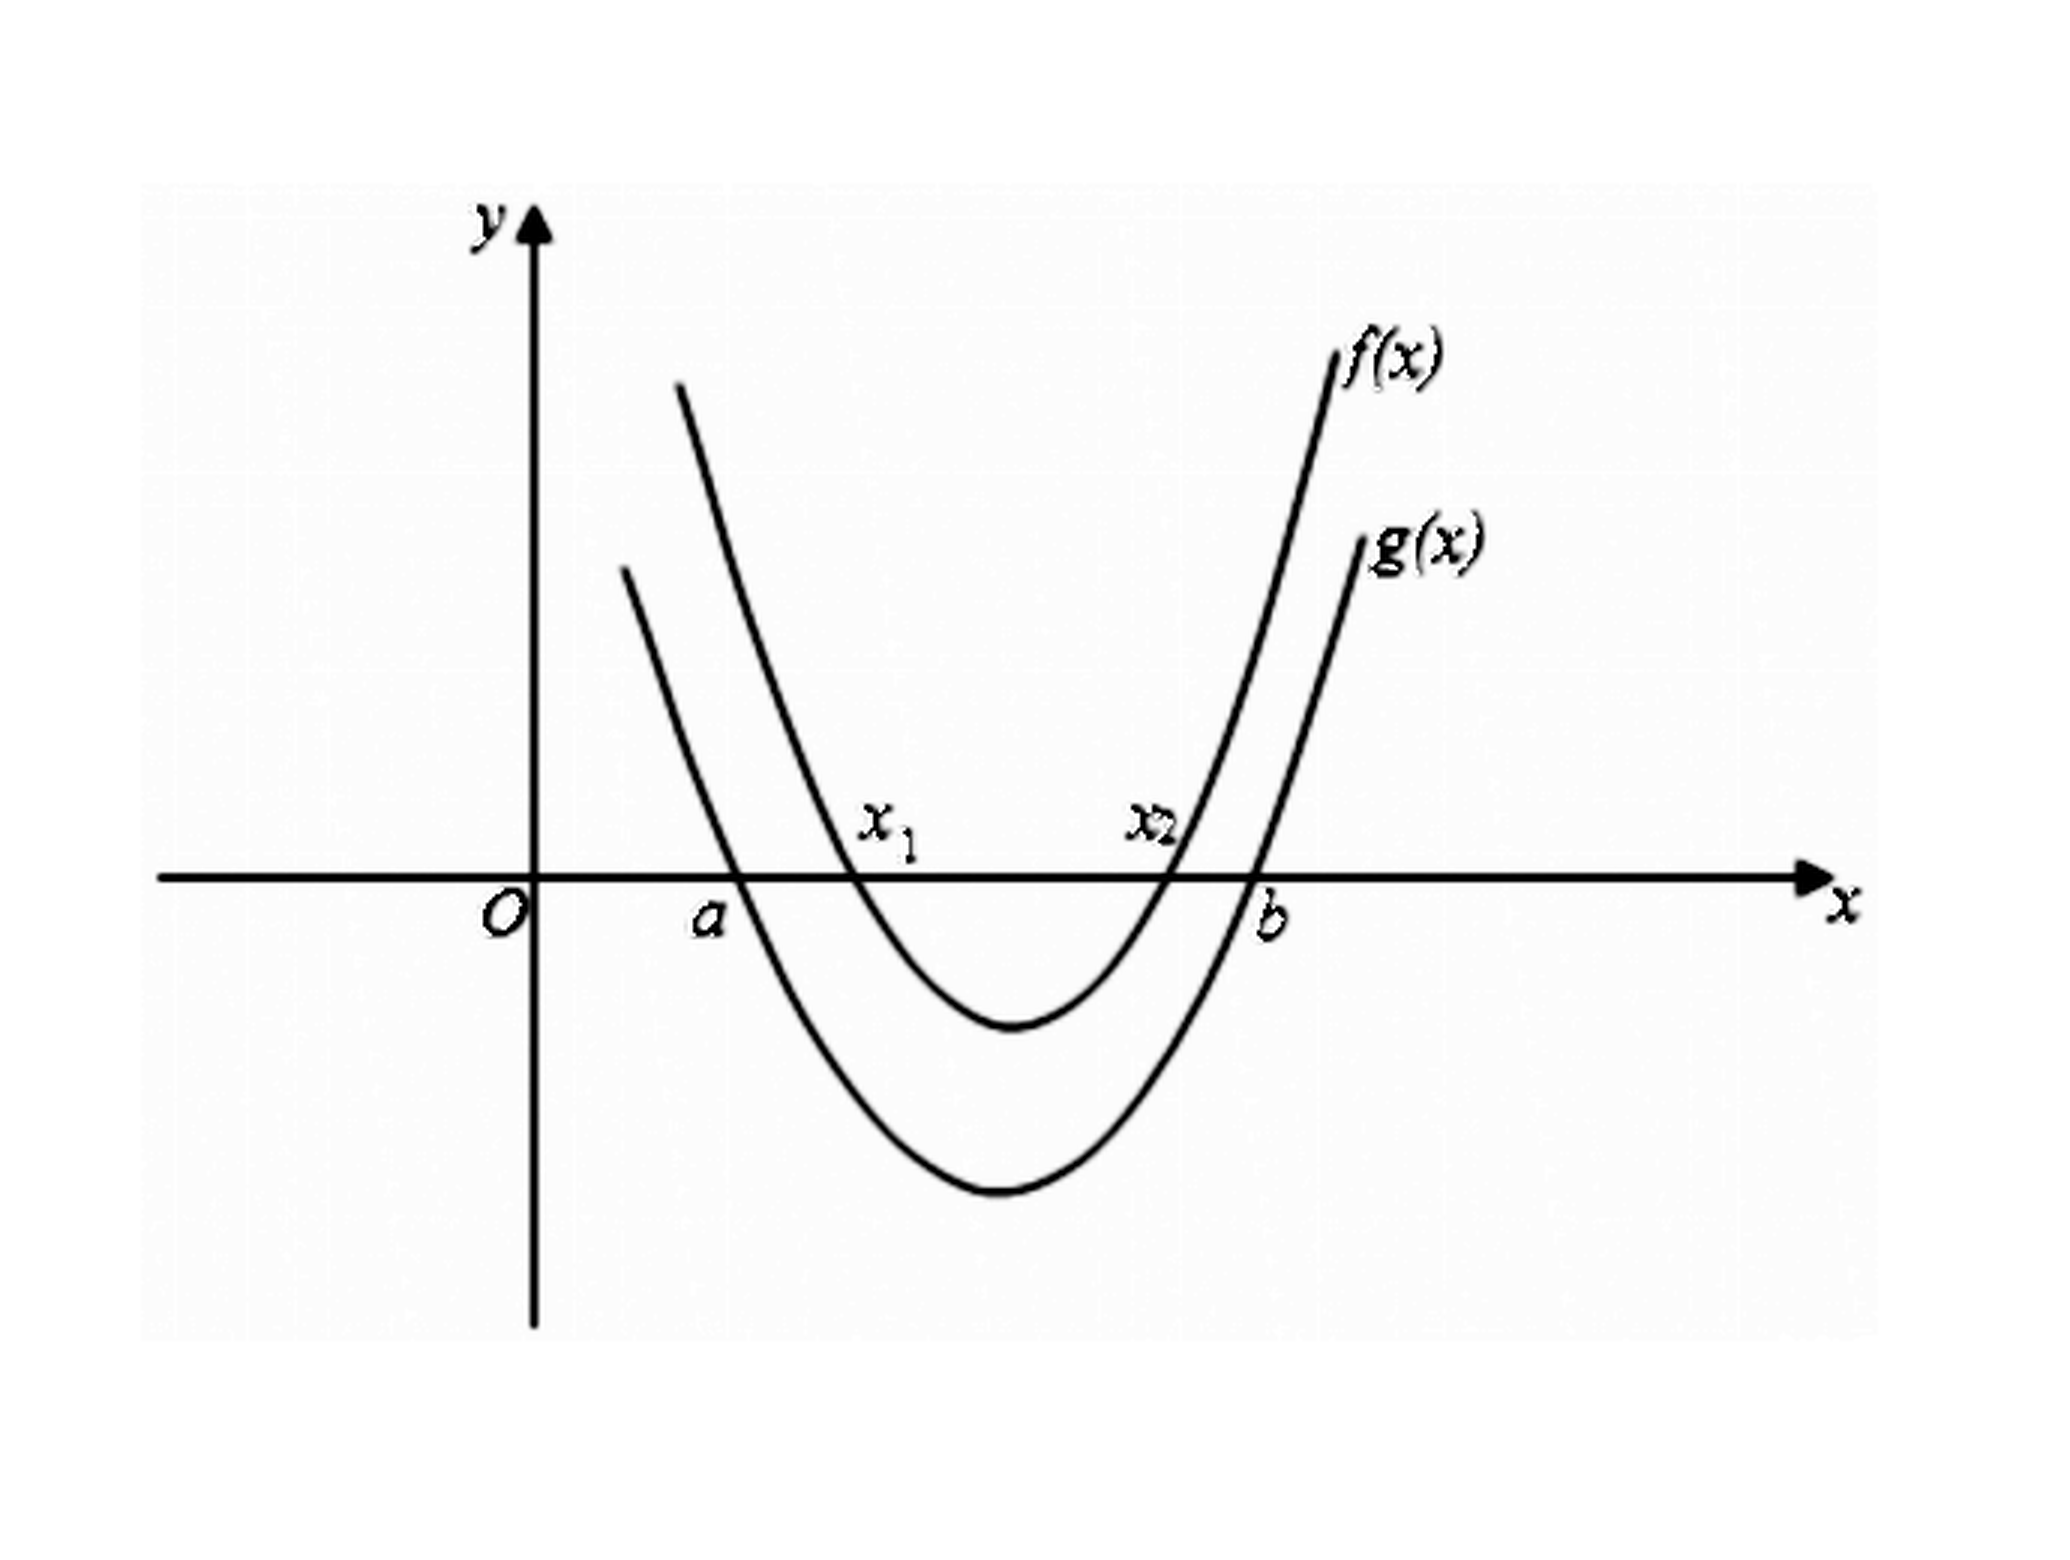
\includegraphics[width=0.52\textwidth]{figures/gao157_q16.png}
\end{center}

\step{由图像得 $a<x_1<x_2<b$，故选 $A$.}
\solend
\fi

\end{enumerate}

\bigsec{三、解答题}

\begin{enumerate}
\setcounter{enumi}{16}

% === Q17 === 解析 6 行；\overline{A}、\varnothing、\subseteq 无、cases
\item 设全集为 $\R$，$m\in\R$，集合 $A=\{x\mid 2<x<5\}$，$B=\{x\mid 2m\leqslant x\leqslant 5m-3\}$.

(1) 若 $m=2$，求 $\overline{A}\cup B$；

(2) 若 $A\cap B=B$，求 $m$ 的取值范围.

\ifanswer
\solbegin
\step{(1) $\overline{A}=\{x\mid x\leqslant2$ 或 $x\geqslant5\}$，当 $m=2$ 时，$B=\{x\mid 4\leqslant x\leqslant7\}$，}
\step{则 $\overline{A}\cup B=\{x\mid x\leqslant2$ 或 $x\geqslant4\}$；}
\step{(2) 因为 $A\cap B=B$，所以 $B$ 是 $A$ 的子集，}
\step{当 $B=\varnothing$ 时，$2m>5m-3$，解得 $m<1$；}
\step{当 $B\ne\varnothing$ 时，$\begin{cases}2m\leqslant5m-3\\2m>2\\5m-3<5\end{cases}$，解得 $1<m<\dfrac85$；}
\step{综上，$m$ 的取值范围是 $(-\infty,1)\cup\left(1,\dfrac85\right)$.}
\solend
\fi

% === Q18 === 解析 2 行；指数式、\lg、换底
\item (1) 设 $a^{2x}=3$，且 $a>0$，求 $\dfrac{a^{3x}+a^{-3x}}{a^x+a^{-x}}$ 的值；

(2) 已知 $\lg2=a, 10^b=3$，用 $a$ 及 $b$ 表示 $\log_{12}25$.

\ifanswer
\solbegin
\step{(1) $\dfrac{a^{3x}+a^{-3x}}{a^x+a^{-x}}=a^{2x}-1+a^{-2x}=3-1+\dfrac13=\dfrac73$；}
\step{(2) $\log_{12}25=\dfrac{\lg25}{\lg12}=\dfrac{2-2\lg2}{2\lg2+\lg3}=\dfrac{2-2a}{2a+b}$.}
\solend
\fi

% === Q19 === 解析 11 行；幂函数、$=0$ 笔误照录、\Delta、\sqrt5、cases
\item 已知幂函数 $f(x)=(m^2+m-1)x^{-2m^2+m+3}$ 在 $(0,+\infty)$ 上为严格增函数.

(1) 求 $f(x)$ 的解析式；

(2) 若 $k+kf(x)>f(x)-x-1$ 对任意实数 $x$ 都成立，求实数 $k$ 的取值范围；

(3) 若关于 $x$ 的不等式 $f(x)\leqslant8x-a$ 的解集中有且仅有 $5$ 个整数，求实数 $a$ 的范围.

\ifanswer
\solbegin
\step{(1) 由题意得 $m^2+m-1=1$，且 $-2m^2+m+3>0$，}
\step{解得 $m=-2$（舍去）或 $m=1$，所以 $f(x)=x^2$；}
\step{(2) $k+kf(x)>f(x)-x-1$ 可化为 $(k-1)x^2+x+k+1=0$ 恒成立，}
\step{当 $k=1$ 时，$x+2>0$，显然不恒成立；}
\step{当 $k\ne1$ 时，要使该二次不等式恒成立，只需 $\begin{cases}k-1>0\\[2pt]\Delta=1-4(k+1)(k-1)\leqslant0\end{cases}$，}
\step{解得 $k\geqslant\dfrac{\sqrt5}{2}$，即所求 $k$ 的范围是 $\left[\dfrac{\sqrt5}{2},+\infty\right)$；}
\step{(3) 不等式 $f(x)\leqslant8x-a$，即 $x^2-8x+a\leqslant0$ 有五个整数解，}
\step{令 $g(x)=x^2-8x+a$，因为该函数开口向上，对称轴为 $x=4$，}
\step{所以解集内的整数为 $2$，$3$，$4$，$5$，$6$，}
\step{由二次函数的性质得，只需 $\begin{cases}g(1)=1-8+a>0\\g(2)=4-8\times2+a\leqslant0\end{cases}$，解得 $7<a\leqslant12$，}
\step{故 $a$ 的取值范围是 $(7,12]$.}
\solend
\fi

% === Q20 === 解析 12 行；材料题、$a+b=1$、大根号、"因出"笔误、分母套分数
\item 问题：正数 $a$、$b$ 满足 $a+b=1$，求 $\dfrac1a+\dfrac2b$ 的最小值.

其中一种解法是：$\dfrac1a+\dfrac2b=\left(\dfrac1a+\dfrac2b\right)(a+b)=1+\dfrac ba+\dfrac{2a}{b}+2\geqslant3+2\sqrt2$，

当且仅当 $\dfrac ba=\dfrac{2a}{b}$ 且 $a+b=1$ 时，即 $a=\sqrt2-1$ 且 $b=2-\sqrt2$ 时取等号.

学习上述解法并解决下列问题：

(1) 若正实数 $x$、$y$ 满足 $x+y=1$，求 $\dfrac2x+\dfrac1y$ 的最小值；

(2) 若实数 $a$、$b$、$x$、$y$ 满足 $\dfrac{x^2}{a^2}-\dfrac{y^2}{b^2}=1$，求证：$a^2-b^2\leqslant(x-y)^2$；

(3) 利用 (2) 的结论，求代数式 $M=\sqrt{2m-5}-\sqrt{m-3}$ 的最小值，并求出使得 $M$ 最小的 $m$ 的值.

\ifanswer
\solbegin
\step{(1) $\dfrac2x+\dfrac1y=(x+y)\left(\dfrac2x+\dfrac1y\right)=3+\dfrac xy+\dfrac{2y}{x}\geqslant3+2\sqrt2$，}
\step{当且仅当 $\dfrac xy=\dfrac{2y}{x}$ 且 $x+y=1$ 时取等号；}
\step{(2) $a^2-b^2=(a^2-b^2)\left(\dfrac{x^2}{a^2}-\dfrac{y^2}{b^2}\right)=x^2+y^2-\left(\dfrac{a^2x^2}{b^2}+\dfrac{b^2y^2}{a^2}\right)$}
\step{$\leqslant x^2+y^2-2\sqrt{\dfrac{a^2x^2}{b^2}\cdot\dfrac{b^2y^2}{a^2}}=x^2+y^2-2xy=(x-y)^2$，}
\step{故当 $b^4x^2=a^4y^2$ 时，等号成立.}
\step{(3) 令 $x=\sqrt{2m-5}, y=\sqrt{m-3}$，由 $\begin{cases}2m-5\geqslant0\\m-3\geqslant0\end{cases}$ 得 $m\geqslant3$，}
\step{$x^2-y^2=(2m-5)-(m-3)=m-2>0$，}
\step{又 $x>0, y>0$，所以 $x>y$，所以 $\dfrac{x^2}{a^2}-\dfrac{y^2}{b^2}=1$，}
\step{由 $x^2-2y^2=1$，得 $\dfrac{x^2}{1}-\dfrac{y^2}{\frac12}=1$，因出 $a^2=1, b^2=\dfrac12$，}
\step{由 (2) 得 $M=\sqrt{2m-5}-\sqrt{m-3}=x-y\geqslant\sqrt{a^2-b^2}=\sqrt{1-\dfrac12}=\dfrac{\sqrt2}{2}$，}
\step{当且仅当 $\dfrac xy=\left(\dfrac ab\right)^2=2$ 取等号，结合 $x^2-2y^2=1$，解得 $x=\sqrt2, y=\dfrac{\sqrt2}{2}$，}
\step{即 $\sqrt{2m-5}=\sqrt2$，得 $m=\dfrac72$，所以 $m=\dfrac72$ 时，$M$ 取得最小值 $\dfrac{\sqrt2}{2}$.}
\solend
\fi

\end{enumerate}

\end{document}
"
%
% ① 原始材料：微信公众号"魔都数学加油站"文章，连载"27学年高一157"，原文标题
% "27学年高一157——2026-2027年上海市大境中学高一上期中"；
% 原文链接：https://mp.weixin.qq.com/s/s6eDMDVkxc2fcBe8LNm-Tw 。
% 正文为 8 张 PNG 页（01/02/03/04/06 为 4762×6735，05/07/08 为 2560×3620，
% 同一篇各页分辨率混排，逐页按各自分辨率裁图核对）。
% 体例：讲评版——填空 3—12（10 题）、选择 13—16（4 题）、解答 17—20（4 题），
% 共 18 题，自第 3 题起编（1、2 未印在本篇）；末题是第 20 题（不是 21）。
% 除第 4 题只印【答案】外，其余 17 题逐题印【解析】（逐题核实，见 ②）。
% 题目、答案、解析均据原图转录；卷面粉红色水印"魔都数学加油站"及公众号
% 页脚未录入。
% 全卷仅 1 幅配图：第 16 题解析内函数图像（"设 g(x)=(x-a)(x-b)，
% f(x)=g(x)+1，画出函数 g(x) 与函数 f(x) 的图像，如图所示"），
% 解析内配图仅答案版出，裁 figures/gao157_q16.png；逐页通读 8 页确认
% 无题目配图、无表格；08 页下半仅水印、无正文。
%
% 卷首标题：原卷印作"2026-2027 年大境中学高一上期中"，年份区间按全稿惯例排 en dash；
% 原卷卷面未印副标题，本稿按同期中卷知识模块口径补出"集合与常用逻辑用语、不等式、函数"。
%
% ② 与原卷的排版差异：
%   ① 原文从第 3 题起，本稿保留原题号；共 18 题三节，解答题 4 题到 20；
%      三节各自 \begin{enumerate}…\end{enumerate} + \setcounter{enumi}{2/12/16}
%      （题目溯源.py 按 \bigsec 切节、每节独立计 depth，只收 depth==1 的 \item，
%       见 高一156 头注②的订正）；
%   ② 第 4 题只印【答案】、无【解析】，提 \ans{}；其余 17 题逐题印【解析】、
%      逐题设 \solbegin…\solend；四道选择题答案在解析末句"故选 D／D／C／A"
%      （逐个放大复核）、括号 \mbox{（\quad）} 留空；答案版【答案】/【解析】
%      标记数 = 18 = 全卷题数（1 个 \ans ＋ 17 个 \solbegin）；
%   ③ 原卷卷面未印副标题，本稿按知识模块口径补出；
%   ④ 原卷填空横线按全稿惯例排 \blankline[4.4em]；选择题选项段前按惯例各加
%      \keepwithprev；解答题不留作答区、不加 \anspace（原卷为讲评版，109—113 起
%      全稿不用 \anspace）；
%   ⑤ 数集：Q4"$x、y\in R$"、Q6"$x\in R$"、Q10"$a\in Z$"、Q12"$n\in Z$"
%      "$n_1、n_2\in Z$"、Q17"全集为 R／$m\in R$"原卷印斜体 R/Z，按全稿惯例
%      归一 \R／\Z（参见 高一14 头注④、高一150 头注②⑤、高一153 头注⑤）；
%      绝对值排 \lvert…\rvert（Q6 $\lvert x-1\rvert$／$\lvert x+3\rvert$／
%      $\lvert 2x+2\rvert$），集合描述竖线排 \mid（Q12、Q17），空集 \varnothing
%      （Q17"$B=\varnothing$"），补集照原卷上划线排 \overline{A}（Q17），
%      不等号按全稿惯例排 \leqslant／\geqslant；
%   ⑥ 判别式三处（Q8"$\Delta=(-2m)^2-4(m+2)$"、Q15"$\Delta=(a+2)^2+4(a^2-4)<0$"、
%      Q19"$\Delta=1-4(k+1)(k-1)\leqslant0$"）放大比对同形、均为等腰偏高且右斜边
%      加粗的 \Delta，统一照录 \Delta；本卷无扁三角 \triangle 用例（与 高一142／
%      高一151／高一152 的 Δ/△ 混用卷不同）；
%   ⑦ "图像／图象"逐处照录不统一：Q9"图像过点 $(4,2)$""它的图像过点"、
%      Q16"画出函数 $g(x)$ 与函数 $f(x)$ 的图像""由图像得"用"图像"；
%      Q14 题干及解析四处均用"图象"（"的图象关于原点对称""图象关于 $y$ 轴对称"）；
%   ⑧ 原卷笔误／未化简式照录：
%      · Q5 解析"$2\sqrt4+1=5$"根号 4 原卷未化简，照录 \sqrt4；
%      · Q7 解析"$\lg\frac{E_1}{E_2}=\frac25\cdot(m_2-m_1)=\frac25(-1.45+26.7)=10.1$"
%        第一处有 \cdot、第二处无，逐处照录；题干"$m_1-m_2=-\frac52\lg\frac{E_1}{E_2}$"；
%      · Q10 解析"$f(1)=\frac{a+1}{1+2}\geqslant0$"与 cases 第二行分母均印 $1+2$、
%        未化简成 $3$，照录；
%      · Q19 (2)"可化为 $(k-1)x^2+x+k+1=0$ 恒成立"原卷印 $=0$（与 >0 恒成立
%        的题意不符），照录笔误；
%      · Q20 (3)"因出 $a^2=1, b^2=\frac12$"原卷印"因出"（当作"因此"），照录；
%      · Q20 (3)"得 $\frac{x^2}{1}-\frac{y^2}{\frac12}=1$"分母套分数、照录；
%   ⑨ 圈数字①②在文本模式（Q15 解析"①当 $a^2-4=0$ 时""②当 $a^2-4\ne0$ 时"，
%      共 2 枚）；子题标号 (1)(2)(3) 半角括号照录；行末西文句点 ASCII `.`；
%      行中全角逗号／顿号照录；半角逗号在数学组之间是全稿惯例、非笔误
%      （Q8"$x_1+x_2=2m, x_1x_2=m+2$"、Q12"$n\in Z$"、Q18"$\lg2=a, 10^b=3$"、
%      Q20"$a^2=1, b^2=\frac12$"等）；中文弯引号""照录（Q4 命题）；
%   ⑩ 自定义名词：Q11"交叉数"、Q12"$a\otimes b$"新定义运算、Q20"问题／
%      其中一种解法是／学习上述解法并解决下列问题"材料题，均照原卷录入；
%   ⑪ 配图：全卷 1 幅（逐页通读 8 页确认）——Q16 解析内函数图像（05 页右侧，
%      $f(x)$ 与 $g(x)$ 两条抛物线、标注 $a,x_1,x_2,b$），仅答案版出，
%      裁 figures/gao157_q16.png，去粉色水印、去色、3× LANCZOS 放大；
%      图放 \ifanswer 内 \solbegin…\solend 的两 \step 之间（高一108 第 6 题／
%      高一156 Q15 成例）；Q16 题干无"如图"、不需题目配图守卫。
%
% ③ 行数复核：一条 \step = 原卷解析的一个印刷行，cases 块作一个印刷行计；
%    跨半页重叠行（Q5 的"【解析】x-1>0…"、Q10 的"所以 a=-1 或 a=0"、
%    Q12 的"【解析】由 u⊗v…"、Q14 的"f(x)=x² 图象关于 y 轴对称"、
%    Q19 的"(1) 由题意得…"、Q20 的"(3) 令 x=…"等 hi_1/hi_2 两半页共有的行）
%    只计一次，别把原卷折行并起来。
%    逐题数（主会话逐页核对定稿）：Q3：1；Q4：0（只印【答案】、提 \ans{}，
%    不计入 \step 账）；Q5：2；Q6：5；Q7：2；Q8：5；Q9：3；Q10：4；
%    Q11：3；Q12：6；Q13：3；Q14：5；Q15：9；Q16：4；Q17：6；Q18：2；
%    Q19：11；Q20：12。合计 83 条 \step（本卷无 \stepm），与原卷逐题印刷行相等。
%    全卷 18 题：1 题只印【答案】（\ans）、17 题印【解析】（\solbegin…\solend），
%    答案版【答案】/【解析】标记数 = 18 = 全卷题数。
%    全卷除此 6 类外未发现其它笔误／自相矛盾处；17 题印【解析】、1 题印【答案】。
%
\documentclass[a4paper,11pt]{article}
\usepackage{common}

\begin{document}

\examtitlest[3]{2026--2027 年大境中学高一上期中}{集合与常用逻辑用语、不等式、函数}

\bigsec{一、填空题}

\begin{enumerate}
\setcounter{enumi}{2}

% === Q3 === 解析 1 行；$a,b$ 半角逗号照录
\item 若 $a=x^2-2x+1$，$b=x-3$，则 $a,b$ 的大小关系为\blankline[4.4em].

\ifanswer
\solbegin
\step{$a-b=x^2-3x+4=\left(x-\dfrac32\right)^2+\dfrac74>0$，所以 $a>b$.}
\solend
\fi

% === Q4 === 只印【答案】、无【解析】；中文弯引号、\R、顿号；提 \ans{}
\item 用反证法证明命题：“设 $x$、$y\in\R$. 若 $x+y>2$，则 $x>1$ 或 $y>1$”时，假设的内容应该是\blankline[4.4em].

\ifanswer
\ans{$x\leqslant1$ 且 $y\leqslant1$}
\fi

% === Q5 === 解析 2 行；$2\sqrt4+1=5$ 根号 4 未化简照录
\item 当 $x>1$ 时，$x+\dfrac4{x-1}$ 的最小值为\blankline[4.4em].

\ifanswer
\solbegin
\step{$x-1>0$，$x+\dfrac4{x-1}=(x-1)+\dfrac4{x-1}+1\geqslant2\sqrt4+1=5$，}
\step{当且仅当 $x-1=\dfrac4{x-1}$，即 $x=3$ 时取等号，故最小值为 $5$.}
\solend
\fi

% === Q6 === 解析 5 行；绝对值 \lvert…\rvert、\cup、\R
\item 设 $x\in\R$，方程 $\lvert x-1\rvert+\lvert x+3\rvert=\lvert 2x+2\rvert$ 的解集是\blankline[4.4em].

\ifanswer
\solbegin
\step{当 $x\leqslant-3$ 时，方程为 $1-x-x-3=-2x-2$，等式成立；}
\step{当 $-3<x\leqslant-1$ 时，方程为 $1-x+x+3=-2x-2$，解得 $x=-3$，舍去；}
\step{当 $-1<x<1$ 时，方程为 $1-x+x+3=2x+2$，解得 $x=1$，舍去；}
\step{当 $x\geqslant1$ 时，方程为 $x-1+x+3=2x+2$，等式成立，}
\step{综上，方程 $\lvert x-1\rvert+\lvert x+3\rvert=\lvert 2x+2\rvert$ 的解集为 $(-\infty,-3]\cup[1,+\infty)$.}
\solend
\fi

% === Q7 === 解析 2 行；星等材料题、\lg、\cdot 逐处照录、天狼星
\item 在天文学中，天体的明暗程度可以用星等或亮度来描述，两颗星的星等与亮度满足 $m_1-m_2=-\dfrac52\lg\dfrac{E_1}{E_2}$，其中星等为 $m_k$ 的星的亮度为 $E_k(k=1,2)$. 已知太阳的星等为 $-26.7$，天狼星的星等为 $-1.45$，则太阳与天狼星的亮度的比值为\blankline[4.4em].

\ifanswer
\solbegin
\step{两颗星的星等与亮度满足 $m_1-m_2=-\dfrac52\lg\dfrac{E_1}{E_2}$，令 $m_2=-1.45$，$m_1=-26.7$，}
\step{$\lg\dfrac{E_1}{E_2}=\dfrac25\cdot(m_2-m_1)=\dfrac25(-1.45+26.7)=10.1$，$\dfrac{E_1}{E_2}=10^{10.1}$.}
\solend
\fi

% === Q8 === 解析 5 行；韦达定理、判别式 \Delta、半角逗号在数学组间
\item 已知方程 $x^2-2mx+m+2=0$ 有两个实数根 $x_1,x_2$，满足 $x_1^2+x_2^2=2$，则实数 $m$ 的值为\blankline[4.4em].

\ifanswer
\solbegin
\step{对于方程 $x^2-2mx+m+2=0$，由韦达定理得 $x_1+x_2=2m, x_1x_2=m+2$，}
\step{又 $x_1^2+x_2^2=(x_1+x_2)^2-2x_1x_2=(2m)^2-2(m+2)=4m^2-2m-4=2$，}
\step{解得 $m=\dfrac32$ 或 $m=-1$，}
\step{因为方程有两个实数根，所以 $\Delta=(-2m)^2-4(m+2)=4m^2-4m-8\geqslant0$，}
\step{解得 $m\leqslant-1$ 或 $m\geqslant2$，故 $m=-1$.}
\solend
\fi

% === Q9 === 解析 3 行；"图像"照录、$x^\alpha$、$x^{1/2}=\sqrt{x}$
\item 已知幂函数 $y=f(x)$ 的图像过点 $(4,2)$，则不等式 $f(x^2-2x)<f(2-x)$ 的解集为\blankline[4.4em].

\ifanswer
\solbegin
\step{设幂函数 $y=f(x)=x^\alpha$，它的图像过点 $(4,2)$，所以 $4^\alpha=2$，$\alpha=\dfrac12$，}
\step{故 $f(x)=x^{\frac12}=\sqrt{x}$，由不等式 $f(x^2-2x)<f(2-x)$，}
\step{得 $0\leqslant x^2-2x<2-x$，得 $-1<x\leqslant0$，故解集为 $(-1,0]$.}
\solend
\fi

% === Q10 === 解析 4 行；$a\in\Z$、cases（分母 $1+2$ 未化简）、参数分离
\item 已知函数 $y=\dfrac{ax+1}{x+2}$（常数 $a\in\Z$）. 要使该函数在区间 $[1,+\infty)$ 上是严格减函数，并且函数值不恒为负，则满足条件的 $a$ 的取值为\blankline[4.4em].

\ifanswer
\solbegin
\step{函数参数分离为 $y=\dfrac{a(x+2)+1-2a}{x+2}=a+\dfrac{1-2a}{x+2}$，}
\step{若函数在区间 $[1,+\infty)$ 上严格减函数，则 $1-2a>0$，}
\step{且函数的最大值 $f(1)=\dfrac{a+1}{1+2}\geqslant0$，即 $\begin{cases}1-2a>0\\[2pt]\dfrac{a+1}{1+2}\geqslant0\end{cases}$，解得 $-1\leqslant a<\dfrac12$，又 $a\in\Z$，}
\step{所以 $a=-1$ 或 $a=0$.}
\solend
\fi

% === Q11 === 解析 3 行；"交叉数"自定义名词、$(-1)^t$、$2^5$、$32\times3=96$
\item 对非空集合 $A$ 中的每个元素 $t$，都乘以 $(-1)^t$ 再求和，称为集合 $A$ 的交叉数，例如 $A=\{2,3,6\}$，则集合 $A$ 的交叉数为 $(-1)^2\cdot2+(-1)^3\cdot3+(-1)^6\cdot6=5$. 若集合 $W=\{1,2,3,4,5,6\}$，则 $W$ 的所有非空子集的交叉数的总和为\blankline[4.4em].

\ifanswer
\solbegin
\step{固定 $W$ 中的任一元素，其余 $5$ 个元素各有选或不选两种情况，}
\step{因此该元素出现在 $2^5$ 个非空子集中，}
\step{所有交叉数的总和为 $2^5(-1+2-3+4-5+6)=32\times3=96$.}
\solend
\fi

% === Q12 === 解析 6 行；\otimes、\lambda、\mid、\Z、\times 与 \cdot 逐处照录
\item 对于任意两个正实数 $a$、$b$，定义 $a\otimes b=\lambda\cdot\dfrac ab$，其中常数 $\lambda\in\left(\dfrac{\sqrt2}{2},1\right)$. 若 $u\geqslant v>0$，且 $u\otimes v$ 与 $v\otimes u$ 都是集合 $\left\{x\mid x=\dfrac n2,n\in\Z\right\}$ 的元素，则 $u\otimes v=$\blankline[4.4em].

\ifanswer
\solbegin
\step{由 $u\otimes v$ 与 $v\otimes u$ 都是集合 $\left\{x\mid x=\dfrac n2,n\in\Z\right\}$ 的元素，}
\step{不妨设 $\lambda\times\dfrac uv=\dfrac12 n_1$，$\lambda\times\dfrac vu=\dfrac12 n_2$，$n_1$、$n_2\in\Z$，}
\step{因为 $u\geqslant v>0$，所以 $0<\dfrac vu\leqslant1$，因为 $\lambda\in\left(\dfrac{\sqrt2}{2},1\right)$，所以 $\dfrac12 n_2=\lambda\cdot\dfrac vu\in(0,1)$，}
\step{因为 $n_2\in\Z$，所以 $n_2=1$，即 $\dfrac12=\dfrac{\lambda v}{u}$，所以 $\lambda=\dfrac{u}{2v}\in\left(\dfrac{\sqrt2}{2},1\right)$，}
\step{所以 $\dfrac uv\in(\sqrt2,2)$，$\dfrac{u^2}{v^2}\in(2,4)$，则 $\lambda\cdot\dfrac uv=\dfrac{u^2}{v^2}\times\dfrac12=\dfrac12 n_1\in(1,2)$，}
\step{因为 $n_1\in\Z$，所以 $n_1=3$，$\dfrac12 n_1=\dfrac32$，故 $u\otimes v=\dfrac32$.}
\solend
\fi

\end{enumerate}

\bigsec{二、选择题}

\begin{enumerate}
\setcounter{enumi}{12}

% === Q13 === 解析 3 行；选项段 \keepwithprev；故选 D
\item 下列不等式成立的为\mbox{（\quad）}

\keepwithprev
A. 若 $a>b$，则 $ac^2>bc^2$\qquad B. 若 $a>b$，则 $a^2>b^2$

C. 若 $a>b$，$c>d$，则 $a+b>c+d$\qquad D. 若 $a>b$，则 $a^3>b^3$

\ifanswer
\solbegin
\step{A 中 $c=0$ 时不成立；B 取 $a=1$，$b=-2$ 不成立；}
\step{C 取 $a=1$，$b=0$，$c=5$，$d=0$ 不成立.}
\step{幂函数 $y=x^3$ 在实数集上严格递增，所以 $a>b\Rightarrow a^3>b^3$，故选 $D$.}
\solend
\fi

% === Q14 === 解析 5 行；"图象"四处照录；故选 D
\item 幂函数 $f(x)=x^\alpha$ 的图象关于原点对称，且在 $(-\infty,0)$ 上是严格增函数，则 $f(x)$ 可以是\mbox{（\quad）}

\keepwithprev
A. $f(x)=x^{-1}$\qquad B. $f(x)=x^{\frac12}$\qquad C. $f(x)=x^2$\qquad D. $f(x)=x^3$

\ifanswer
\solbegin
\step{$f(x)=\dfrac1x$ 的图象关于原点对称，在 $(-\infty,0)$ 上是严格减函数，故 $A$ 错误；}
\step{$f(x)=x^{\frac12}$ 在 $(-\infty,0)$ 上无意义，故 $B$ 错误；}
\step{$f(x)=x^2$ 图象关于 $y$ 轴对称，故 $C$ 错误；}
\step{$f(x)=x^3$ 的图象关于原点对称，且在 $(-\infty,0)$ 上是严格增函数，故 $D$ 正确.}
\step{故选 $D$.}
\solend
\fi

% === Q15 === 解析 9 行；圈数字①②、\Delta、cases；故选 C
\item 若关于 $x$ 的不等式 $(a^2-4)x^2+(a+2)x-1\geqslant0$ 的解集不为空集，则实数 $a$ 的取值范围为\mbox{（\quad）}

\keepwithprev
A. $\left(-2,\dfrac65\right]$\qquad B. $\left[-2,\dfrac65\right]$

C. $(-\infty,-2)\cup\left[\dfrac65,+\infty\right)$\qquad D. $(-\infty,-2]\cup\left[\dfrac65,+\infty\right)$

\ifanswer
\solbegin
\step{①当 $a^2-4=0$ 时，$a=\pm2$，}
\step{若 $a=2$ 时，原不等式为 $4x-1\geqslant0$，则不等式的解集不是空集；}
\step{若 $a=-2$ 时，原不等式为 $-1\geqslant0$，无解，不符合题意；}
\step{②当 $a^2-4\ne0$ 时，$a\ne\pm2$，}
\step{若 $(a^2-4)x^2+(a+2)x-1\geqslant0$ 的解集是空集，则 $\begin{cases}a^2-4<0\\[2pt]\Delta=(a+2)^2+4(a^2-4)<0\end{cases}$，}
\step{解得 $-2<a<\dfrac65$，}
\step{则当不等式 $(a^2-4)x^2+(a+2)x-1\geqslant0$ 的解集不为空集时，}
\step{有 $a<-2$ 或 $a\geqslant\dfrac65$ 且 $a\ne2$，}
\step{综上，实数 $a$ 的取值范围为 $(-\infty,-2)\cup\left[\dfrac65,+\infty\right)$，故选 $C$.}
\solend
\fi

% === Q16 === 解析 4 行＋1 幅解析内配图（仅答案版）；"图像"照录；故选 A
\item 已知实数 $a<b$，关于 $x$ 的不等式 $x^2-(a+b)x+ab+1<0$ 的解集为 $(x_1,x_2)$，则实数 $a$、$b$、$x_1$、$x_2$ 从小到大的排列是\mbox{（\quad）}

\keepwithprev
A. $a<x_1<x_2<b$\qquad B. $x_1<a<b<x_2$\qquad C. $a<x_1<b<x_2$\qquad D. $x_1<a<x_2<b$

\ifanswer
\solbegin
\step{不等式 $x^2-(a+b)x+ab+1<0$ 可化为 $(x-a)(x-b)+1<0$，}
\step{设 $g(x)=(x-a)(x-b)$，$f(x)=g(x)+1$，}
\step{画出函数 $g(x)$ 与函数 $f(x)$ 的图像，如图所示，}

\begin{center}
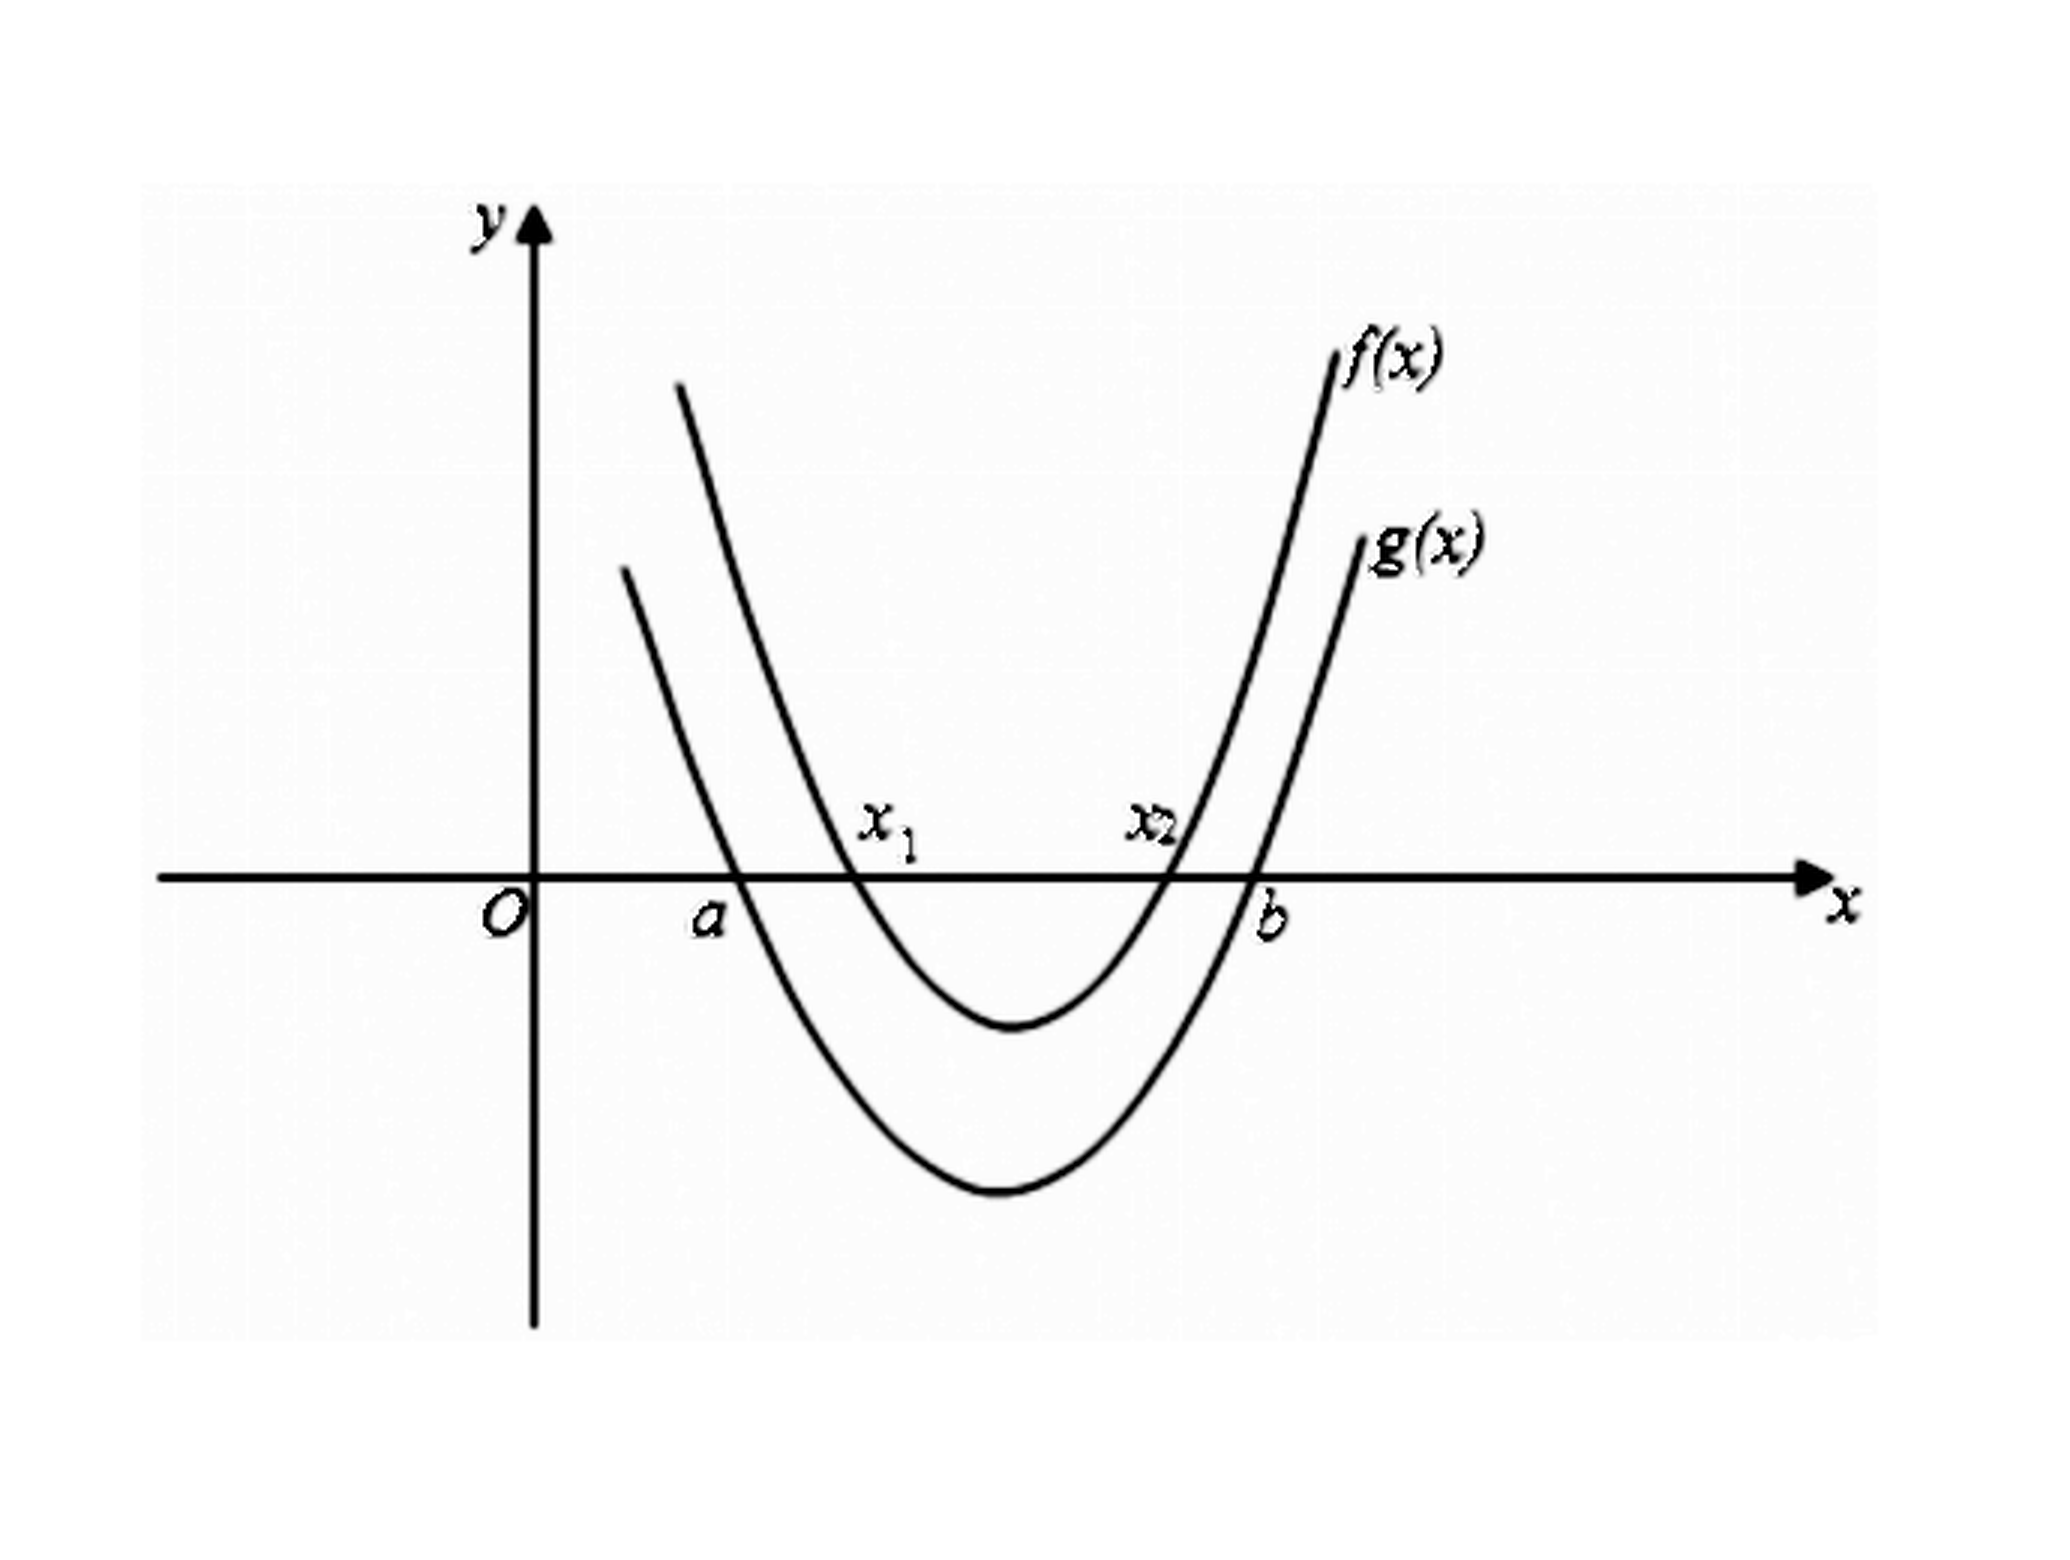
\includegraphics[width=0.52\textwidth]{figures/gao157_q16.png}
\end{center}

\step{由图像得 $a<x_1<x_2<b$，故选 $A$.}
\solend
\fi

\end{enumerate}

\bigsec{三、解答题}

\begin{enumerate}
\setcounter{enumi}{16}

% === Q17 === 解析 6 行；\overline{A}、\varnothing、\subseteq 无、cases
\item 设全集为 $\R$，$m\in\R$，集合 $A=\{x\mid 2<x<5\}$，$B=\{x\mid 2m\leqslant x\leqslant 5m-3\}$.

(1) 若 $m=2$，求 $\overline{A}\cup B$；

(2) 若 $A\cap B=B$，求 $m$ 的取值范围.

\ifanswer
\solbegin
\step{(1) $\overline{A}=\{x\mid x\leqslant2$ 或 $x\geqslant5\}$，当 $m=2$ 时，$B=\{x\mid 4\leqslant x\leqslant7\}$，}
\step{则 $\overline{A}\cup B=\{x\mid x\leqslant2$ 或 $x\geqslant4\}$；}
\step{(2) 因为 $A\cap B=B$，所以 $B$ 是 $A$ 的子集，}
\step{当 $B=\varnothing$ 时，$2m>5m-3$，解得 $m<1$；}
\step{当 $B\ne\varnothing$ 时，$\begin{cases}2m\leqslant5m-3\\2m>2\\5m-3<5\end{cases}$，解得 $1<m<\dfrac85$；}
\step{综上，$m$ 的取值范围是 $(-\infty,1)\cup\left(1,\dfrac85\right)$.}
\solend
\fi

% === Q18 === 解析 2 行；指数式、\lg、换底
\item (1) 设 $a^{2x}=3$，且 $a>0$，求 $\dfrac{a^{3x}+a^{-3x}}{a^x+a^{-x}}$ 的值；

(2) 已知 $\lg2=a, 10^b=3$，用 $a$ 及 $b$ 表示 $\log_{12}25$.

\ifanswer
\solbegin
\step{(1) $\dfrac{a^{3x}+a^{-3x}}{a^x+a^{-x}}=a^{2x}-1+a^{-2x}=3-1+\dfrac13=\dfrac73$；}
\step{(2) $\log_{12}25=\dfrac{\lg25}{\lg12}=\dfrac{2-2\lg2}{2\lg2+\lg3}=\dfrac{2-2a}{2a+b}$.}
\solend
\fi

% === Q19 === 解析 11 行；幂函数、$=0$ 笔误照录、\Delta、\sqrt5、cases
\item 已知幂函数 $f(x)=(m^2+m-1)x^{-2m^2+m+3}$ 在 $(0,+\infty)$ 上为严格增函数.

(1) 求 $f(x)$ 的解析式；

(2) 若 $k+kf(x)>f(x)-x-1$ 对任意实数 $x$ 都成立，求实数 $k$ 的取值范围；

(3) 若关于 $x$ 的不等式 $f(x)\leqslant8x-a$ 的解集中有且仅有 $5$ 个整数，求实数 $a$ 的范围.

\ifanswer
\solbegin
\step{(1) 由题意得 $m^2+m-1=1$，且 $-2m^2+m+3>0$，}
\step{解得 $m=-2$（舍去）或 $m=1$，所以 $f(x)=x^2$；}
\step{(2) $k+kf(x)>f(x)-x-1$ 可化为 $(k-1)x^2+x+k+1=0$ 恒成立，}
\step{当 $k=1$ 时，$x+2>0$，显然不恒成立；}
\step{当 $k\ne1$ 时，要使该二次不等式恒成立，只需 $\begin{cases}k-1>0\\[2pt]\Delta=1-4(k+1)(k-1)\leqslant0\end{cases}$，}
\step{解得 $k\geqslant\dfrac{\sqrt5}{2}$，即所求 $k$ 的范围是 $\left[\dfrac{\sqrt5}{2},+\infty\right)$；}
\step{(3) 不等式 $f(x)\leqslant8x-a$，即 $x^2-8x+a\leqslant0$ 有五个整数解，}
\step{令 $g(x)=x^2-8x+a$，因为该函数开口向上，对称轴为 $x=4$，}
\step{所以解集内的整数为 $2$，$3$，$4$，$5$，$6$，}
\step{由二次函数的性质得，只需 $\begin{cases}g(1)=1-8+a>0\\g(2)=4-8\times2+a\leqslant0\end{cases}$，解得 $7<a\leqslant12$，}
\step{故 $a$ 的取值范围是 $(7,12]$.}
\solend
\fi

% === Q20 === 解析 12 行；材料题、$a+b=1$、大根号、"因出"笔误、分母套分数
\item 问题：正数 $a$、$b$ 满足 $a+b=1$，求 $\dfrac1a+\dfrac2b$ 的最小值.

其中一种解法是：$\dfrac1a+\dfrac2b=\left(\dfrac1a+\dfrac2b\right)(a+b)=1+\dfrac ba+\dfrac{2a}{b}+2\geqslant3+2\sqrt2$，

当且仅当 $\dfrac ba=\dfrac{2a}{b}$ 且 $a+b=1$ 时，即 $a=\sqrt2-1$ 且 $b=2-\sqrt2$ 时取等号.

学习上述解法并解决下列问题：

(1) 若正实数 $x$、$y$ 满足 $x+y=1$，求 $\dfrac2x+\dfrac1y$ 的最小值；

(2) 若实数 $a$、$b$、$x$、$y$ 满足 $\dfrac{x^2}{a^2}-\dfrac{y^2}{b^2}=1$，求证：$a^2-b^2\leqslant(x-y)^2$；

(3) 利用 (2) 的结论，求代数式 $M=\sqrt{2m-5}-\sqrt{m-3}$ 的最小值，并求出使得 $M$ 最小的 $m$ 的值.

\ifanswer
\solbegin
\step{(1) $\dfrac2x+\dfrac1y=(x+y)\left(\dfrac2x+\dfrac1y\right)=3+\dfrac xy+\dfrac{2y}{x}\geqslant3+2\sqrt2$，}
\step{当且仅当 $\dfrac xy=\dfrac{2y}{x}$ 且 $x+y=1$ 时取等号；}
\step{(2) $a^2-b^2=(a^2-b^2)\left(\dfrac{x^2}{a^2}-\dfrac{y^2}{b^2}\right)=x^2+y^2-\left(\dfrac{a^2x^2}{b^2}+\dfrac{b^2y^2}{a^2}\right)$}
\step{$\leqslant x^2+y^2-2\sqrt{\dfrac{a^2x^2}{b^2}\cdot\dfrac{b^2y^2}{a^2}}=x^2+y^2-2xy=(x-y)^2$，}
\step{故当 $b^4x^2=a^4y^2$ 时，等号成立.}
\step{(3) 令 $x=\sqrt{2m-5}, y=\sqrt{m-3}$，由 $\begin{cases}2m-5\geqslant0\\m-3\geqslant0\end{cases}$ 得 $m\geqslant3$，}
\step{$x^2-y^2=(2m-5)-(m-3)=m-2>0$，}
\step{又 $x>0, y>0$，所以 $x>y$，所以 $\dfrac{x^2}{a^2}-\dfrac{y^2}{b^2}=1$，}
\step{由 $x^2-2y^2=1$，得 $\dfrac{x^2}{1}-\dfrac{y^2}{\frac12}=1$，因出 $a^2=1, b^2=\dfrac12$，}
\step{由 (2) 得 $M=\sqrt{2m-5}-\sqrt{m-3}=x-y\geqslant\sqrt{a^2-b^2}=\sqrt{1-\dfrac12}=\dfrac{\sqrt2}{2}$，}
\step{当且仅当 $\dfrac xy=\left(\dfrac ab\right)^2=2$ 取等号，结合 $x^2-2y^2=1$，解得 $x=\sqrt2, y=\dfrac{\sqrt2}{2}$，}
\step{即 $\sqrt{2m-5}=\sqrt2$，得 $m=\dfrac72$，所以 $m=\dfrac72$ 时，$M$ 取得最小值 $\dfrac{\sqrt2}{2}$.}
\solend
\fi

\end{enumerate}

\end{document}
"
% 紧凑版：xelatex "\def\iscompact{1}% 高一157_大境中学_期中.tex
%   —— 高一上数学"2026-2027 年大境中学高一上期中"（试卷版/答案版/紧凑版）
% 试卷版：xelatex 高一157_大境中学_期中.tex
% 答案版：xelatex "\def\isanswer{1}% 高一157_大境中学_期中.tex
%   —— 高一上数学"2026-2027 年大境中学高一上期中"（试卷版/答案版/紧凑版）
% 试卷版：xelatex 高一157_大境中学_期中.tex
% 答案版：xelatex "\def\isanswer{1}\input{高一157_大境中学_期中.tex}"
% 紧凑版：xelatex "\def\iscompact{1}\input{高一157_大境中学_期中.tex}"
%
% ① 原始材料：微信公众号"魔都数学加油站"文章，连载"27学年高一157"，原文标题
% "27学年高一157——2026-2027年上海市大境中学高一上期中"；
% 原文链接：https://mp.weixin.qq.com/s/s6eDMDVkxc2fcBe8LNm-Tw 。
% 正文为 8 张 PNG 页（01/02/03/04/06 为 4762×6735，05/07/08 为 2560×3620，
% 同一篇各页分辨率混排，逐页按各自分辨率裁图核对）。
% 体例：讲评版——填空 3—12（10 题）、选择 13—16（4 题）、解答 17—20（4 题），
% 共 18 题，自第 3 题起编（1、2 未印在本篇）；末题是第 20 题（不是 21）。
% 除第 4 题只印【答案】外，其余 17 题逐题印【解析】（逐题核实，见 ②）。
% 题目、答案、解析均据原图转录；卷面粉红色水印"魔都数学加油站"及公众号
% 页脚未录入。
% 全卷仅 1 幅配图：第 16 题解析内函数图像（"设 g(x)=(x-a)(x-b)，
% f(x)=g(x)+1，画出函数 g(x) 与函数 f(x) 的图像，如图所示"），
% 解析内配图仅答案版出，裁 figures/gao157_q16.png；逐页通读 8 页确认
% 无题目配图、无表格；08 页下半仅水印、无正文。
%
% 卷首标题：原卷印作"2026-2027 年大境中学高一上期中"，年份区间按全稿惯例排 en dash；
% 原卷卷面未印副标题，本稿按同期中卷知识模块口径补出"集合与常用逻辑用语、不等式、函数"。
%
% ② 与原卷的排版差异：
%   ① 原文从第 3 题起，本稿保留原题号；共 18 题三节，解答题 4 题到 20；
%      三节各自 \begin{enumerate}…\end{enumerate} + \setcounter{enumi}{2/12/16}
%      （题目溯源.py 按 \bigsec 切节、每节独立计 depth，只收 depth==1 的 \item，
%       见 高一156 头注②的订正）；
%   ② 第 4 题只印【答案】、无【解析】，提 \ans{}；其余 17 题逐题印【解析】、
%      逐题设 \solbegin…\solend；四道选择题答案在解析末句"故选 D／D／C／A"
%      （逐个放大复核）、括号 \mbox{（\quad）} 留空；答案版【答案】/【解析】
%      标记数 = 18 = 全卷题数（1 个 \ans ＋ 17 个 \solbegin）；
%   ③ 原卷卷面未印副标题，本稿按知识模块口径补出；
%   ④ 原卷填空横线按全稿惯例排 \blankline[4.4em]；选择题选项段前按惯例各加
%      \keepwithprev；解答题不留作答区、不加 \anspace（原卷为讲评版，109—113 起
%      全稿不用 \anspace）；
%   ⑤ 数集：Q4"$x、y\in R$"、Q6"$x\in R$"、Q10"$a\in Z$"、Q12"$n\in Z$"
%      "$n_1、n_2\in Z$"、Q17"全集为 R／$m\in R$"原卷印斜体 R/Z，按全稿惯例
%      归一 \R／\Z（参见 高一14 头注④、高一150 头注②⑤、高一153 头注⑤）；
%      绝对值排 \lvert…\rvert（Q6 $\lvert x-1\rvert$／$\lvert x+3\rvert$／
%      $\lvert 2x+2\rvert$），集合描述竖线排 \mid（Q12、Q17），空集 \varnothing
%      （Q17"$B=\varnothing$"），补集照原卷上划线排 \overline{A}（Q17），
%      不等号按全稿惯例排 \leqslant／\geqslant；
%   ⑥ 判别式三处（Q8"$\Delta=(-2m)^2-4(m+2)$"、Q15"$\Delta=(a+2)^2+4(a^2-4)<0$"、
%      Q19"$\Delta=1-4(k+1)(k-1)\leqslant0$"）放大比对同形、均为等腰偏高且右斜边
%      加粗的 \Delta，统一照录 \Delta；本卷无扁三角 \triangle 用例（与 高一142／
%      高一151／高一152 的 Δ/△ 混用卷不同）；
%   ⑦ "图像／图象"逐处照录不统一：Q9"图像过点 $(4,2)$""它的图像过点"、
%      Q16"画出函数 $g(x)$ 与函数 $f(x)$ 的图像""由图像得"用"图像"；
%      Q14 题干及解析四处均用"图象"（"的图象关于原点对称""图象关于 $y$ 轴对称"）；
%   ⑧ 原卷笔误／未化简式照录：
%      · Q5 解析"$2\sqrt4+1=5$"根号 4 原卷未化简，照录 \sqrt4；
%      · Q7 解析"$\lg\frac{E_1}{E_2}=\frac25\cdot(m_2-m_1)=\frac25(-1.45+26.7)=10.1$"
%        第一处有 \cdot、第二处无，逐处照录；题干"$m_1-m_2=-\frac52\lg\frac{E_1}{E_2}$"；
%      · Q10 解析"$f(1)=\frac{a+1}{1+2}\geqslant0$"与 cases 第二行分母均印 $1+2$、
%        未化简成 $3$，照录；
%      · Q19 (2)"可化为 $(k-1)x^2+x+k+1=0$ 恒成立"原卷印 $=0$（与 >0 恒成立
%        的题意不符），照录笔误；
%      · Q20 (3)"因出 $a^2=1, b^2=\frac12$"原卷印"因出"（当作"因此"），照录；
%      · Q20 (3)"得 $\frac{x^2}{1}-\frac{y^2}{\frac12}=1$"分母套分数、照录；
%   ⑨ 圈数字①②在文本模式（Q15 解析"①当 $a^2-4=0$ 时""②当 $a^2-4\ne0$ 时"，
%      共 2 枚）；子题标号 (1)(2)(3) 半角括号照录；行末西文句点 ASCII `.`；
%      行中全角逗号／顿号照录；半角逗号在数学组之间是全稿惯例、非笔误
%      （Q8"$x_1+x_2=2m, x_1x_2=m+2$"、Q12"$n\in Z$"、Q18"$\lg2=a, 10^b=3$"、
%      Q20"$a^2=1, b^2=\frac12$"等）；中文弯引号""照录（Q4 命题）；
%   ⑩ 自定义名词：Q11"交叉数"、Q12"$a\otimes b$"新定义运算、Q20"问题／
%      其中一种解法是／学习上述解法并解决下列问题"材料题，均照原卷录入；
%   ⑪ 配图：全卷 1 幅（逐页通读 8 页确认）——Q16 解析内函数图像（05 页右侧，
%      $f(x)$ 与 $g(x)$ 两条抛物线、标注 $a,x_1,x_2,b$），仅答案版出，
%      裁 figures/gao157_q16.png，去粉色水印、去色、3× LANCZOS 放大；
%      图放 \ifanswer 内 \solbegin…\solend 的两 \step 之间（高一108 第 6 题／
%      高一156 Q15 成例）；Q16 题干无"如图"、不需题目配图守卫。
%
% ③ 行数复核：一条 \step = 原卷解析的一个印刷行，cases 块作一个印刷行计；
%    跨半页重叠行（Q5 的"【解析】x-1>0…"、Q10 的"所以 a=-1 或 a=0"、
%    Q12 的"【解析】由 u⊗v…"、Q14 的"f(x)=x² 图象关于 y 轴对称"、
%    Q19 的"(1) 由题意得…"、Q20 的"(3) 令 x=…"等 hi_1/hi_2 两半页共有的行）
%    只计一次，别把原卷折行并起来。
%    逐题数（主会话逐页核对定稿）：Q3：1；Q4：0（只印【答案】、提 \ans{}，
%    不计入 \step 账）；Q5：2；Q6：5；Q7：2；Q8：5；Q9：3；Q10：4；
%    Q11：3；Q12：6；Q13：3；Q14：5；Q15：9；Q16：4；Q17：6；Q18：2；
%    Q19：11；Q20：12。合计 83 条 \step（本卷无 \stepm），与原卷逐题印刷行相等。
%    全卷 18 题：1 题只印【答案】（\ans）、17 题印【解析】（\solbegin…\solend），
%    答案版【答案】/【解析】标记数 = 18 = 全卷题数。
%    全卷除此 6 类外未发现其它笔误／自相矛盾处；17 题印【解析】、1 题印【答案】。
%
\documentclass[a4paper,11pt]{article}
\usepackage{common}

\begin{document}

\examtitlest[3]{2026--2027 年大境中学高一上期中}{集合与常用逻辑用语、不等式、函数}

\bigsec{一、填空题}

\begin{enumerate}
\setcounter{enumi}{2}

% === Q3 === 解析 1 行；$a,b$ 半角逗号照录
\item 若 $a=x^2-2x+1$，$b=x-3$，则 $a,b$ 的大小关系为\blankline[4.4em].

\ifanswer
\solbegin
\step{$a-b=x^2-3x+4=\left(x-\dfrac32\right)^2+\dfrac74>0$，所以 $a>b$.}
\solend
\fi

% === Q4 === 只印【答案】、无【解析】；中文弯引号、\R、顿号；提 \ans{}
\item 用反证法证明命题：“设 $x$、$y\in\R$. 若 $x+y>2$，则 $x>1$ 或 $y>1$”时，假设的内容应该是\blankline[4.4em].

\ifanswer
\ans{$x\leqslant1$ 且 $y\leqslant1$}
\fi

% === Q5 === 解析 2 行；$2\sqrt4+1=5$ 根号 4 未化简照录
\item 当 $x>1$ 时，$x+\dfrac4{x-1}$ 的最小值为\blankline[4.4em].

\ifanswer
\solbegin
\step{$x-1>0$，$x+\dfrac4{x-1}=(x-1)+\dfrac4{x-1}+1\geqslant2\sqrt4+1=5$，}
\step{当且仅当 $x-1=\dfrac4{x-1}$，即 $x=3$ 时取等号，故最小值为 $5$.}
\solend
\fi

% === Q6 === 解析 5 行；绝对值 \lvert…\rvert、\cup、\R
\item 设 $x\in\R$，方程 $\lvert x-1\rvert+\lvert x+3\rvert=\lvert 2x+2\rvert$ 的解集是\blankline[4.4em].

\ifanswer
\solbegin
\step{当 $x\leqslant-3$ 时，方程为 $1-x-x-3=-2x-2$，等式成立；}
\step{当 $-3<x\leqslant-1$ 时，方程为 $1-x+x+3=-2x-2$，解得 $x=-3$，舍去；}
\step{当 $-1<x<1$ 时，方程为 $1-x+x+3=2x+2$，解得 $x=1$，舍去；}
\step{当 $x\geqslant1$ 时，方程为 $x-1+x+3=2x+2$，等式成立，}
\step{综上，方程 $\lvert x-1\rvert+\lvert x+3\rvert=\lvert 2x+2\rvert$ 的解集为 $(-\infty,-3]\cup[1,+\infty)$.}
\solend
\fi

% === Q7 === 解析 2 行；星等材料题、\lg、\cdot 逐处照录、天狼星
\item 在天文学中，天体的明暗程度可以用星等或亮度来描述，两颗星的星等与亮度满足 $m_1-m_2=-\dfrac52\lg\dfrac{E_1}{E_2}$，其中星等为 $m_k$ 的星的亮度为 $E_k(k=1,2)$. 已知太阳的星等为 $-26.7$，天狼星的星等为 $-1.45$，则太阳与天狼星的亮度的比值为\blankline[4.4em].

\ifanswer
\solbegin
\step{两颗星的星等与亮度满足 $m_1-m_2=-\dfrac52\lg\dfrac{E_1}{E_2}$，令 $m_2=-1.45$，$m_1=-26.7$，}
\step{$\lg\dfrac{E_1}{E_2}=\dfrac25\cdot(m_2-m_1)=\dfrac25(-1.45+26.7)=10.1$，$\dfrac{E_1}{E_2}=10^{10.1}$.}
\solend
\fi

% === Q8 === 解析 5 行；韦达定理、判别式 \Delta、半角逗号在数学组间
\item 已知方程 $x^2-2mx+m+2=0$ 有两个实数根 $x_1,x_2$，满足 $x_1^2+x_2^2=2$，则实数 $m$ 的值为\blankline[4.4em].

\ifanswer
\solbegin
\step{对于方程 $x^2-2mx+m+2=0$，由韦达定理得 $x_1+x_2=2m, x_1x_2=m+2$，}
\step{又 $x_1^2+x_2^2=(x_1+x_2)^2-2x_1x_2=(2m)^2-2(m+2)=4m^2-2m-4=2$，}
\step{解得 $m=\dfrac32$ 或 $m=-1$，}
\step{因为方程有两个实数根，所以 $\Delta=(-2m)^2-4(m+2)=4m^2-4m-8\geqslant0$，}
\step{解得 $m\leqslant-1$ 或 $m\geqslant2$，故 $m=-1$.}
\solend
\fi

% === Q9 === 解析 3 行；"图像"照录、$x^\alpha$、$x^{1/2}=\sqrt{x}$
\item 已知幂函数 $y=f(x)$ 的图像过点 $(4,2)$，则不等式 $f(x^2-2x)<f(2-x)$ 的解集为\blankline[4.4em].

\ifanswer
\solbegin
\step{设幂函数 $y=f(x)=x^\alpha$，它的图像过点 $(4,2)$，所以 $4^\alpha=2$，$\alpha=\dfrac12$，}
\step{故 $f(x)=x^{\frac12}=\sqrt{x}$，由不等式 $f(x^2-2x)<f(2-x)$，}
\step{得 $0\leqslant x^2-2x<2-x$，得 $-1<x\leqslant0$，故解集为 $(-1,0]$.}
\solend
\fi

% === Q10 === 解析 4 行；$a\in\Z$、cases（分母 $1+2$ 未化简）、参数分离
\item 已知函数 $y=\dfrac{ax+1}{x+2}$（常数 $a\in\Z$）. 要使该函数在区间 $[1,+\infty)$ 上是严格减函数，并且函数值不恒为负，则满足条件的 $a$ 的取值为\blankline[4.4em].

\ifanswer
\solbegin
\step{函数参数分离为 $y=\dfrac{a(x+2)+1-2a}{x+2}=a+\dfrac{1-2a}{x+2}$，}
\step{若函数在区间 $[1,+\infty)$ 上严格减函数，则 $1-2a>0$，}
\step{且函数的最大值 $f(1)=\dfrac{a+1}{1+2}\geqslant0$，即 $\begin{cases}1-2a>0\\[2pt]\dfrac{a+1}{1+2}\geqslant0\end{cases}$，解得 $-1\leqslant a<\dfrac12$，又 $a\in\Z$，}
\step{所以 $a=-1$ 或 $a=0$.}
\solend
\fi

% === Q11 === 解析 3 行；"交叉数"自定义名词、$(-1)^t$、$2^5$、$32\times3=96$
\item 对非空集合 $A$ 中的每个元素 $t$，都乘以 $(-1)^t$ 再求和，称为集合 $A$ 的交叉数，例如 $A=\{2,3,6\}$，则集合 $A$ 的交叉数为 $(-1)^2\cdot2+(-1)^3\cdot3+(-1)^6\cdot6=5$. 若集合 $W=\{1,2,3,4,5,6\}$，则 $W$ 的所有非空子集的交叉数的总和为\blankline[4.4em].

\ifanswer
\solbegin
\step{固定 $W$ 中的任一元素，其余 $5$ 个元素各有选或不选两种情况，}
\step{因此该元素出现在 $2^5$ 个非空子集中，}
\step{所有交叉数的总和为 $2^5(-1+2-3+4-5+6)=32\times3=96$.}
\solend
\fi

% === Q12 === 解析 6 行；\otimes、\lambda、\mid、\Z、\times 与 \cdot 逐处照录
\item 对于任意两个正实数 $a$、$b$，定义 $a\otimes b=\lambda\cdot\dfrac ab$，其中常数 $\lambda\in\left(\dfrac{\sqrt2}{2},1\right)$. 若 $u\geqslant v>0$，且 $u\otimes v$ 与 $v\otimes u$ 都是集合 $\left\{x\mid x=\dfrac n2,n\in\Z\right\}$ 的元素，则 $u\otimes v=$\blankline[4.4em].

\ifanswer
\solbegin
\step{由 $u\otimes v$ 与 $v\otimes u$ 都是集合 $\left\{x\mid x=\dfrac n2,n\in\Z\right\}$ 的元素，}
\step{不妨设 $\lambda\times\dfrac uv=\dfrac12 n_1$，$\lambda\times\dfrac vu=\dfrac12 n_2$，$n_1$、$n_2\in\Z$，}
\step{因为 $u\geqslant v>0$，所以 $0<\dfrac vu\leqslant1$，因为 $\lambda\in\left(\dfrac{\sqrt2}{2},1\right)$，所以 $\dfrac12 n_2=\lambda\cdot\dfrac vu\in(0,1)$，}
\step{因为 $n_2\in\Z$，所以 $n_2=1$，即 $\dfrac12=\dfrac{\lambda v}{u}$，所以 $\lambda=\dfrac{u}{2v}\in\left(\dfrac{\sqrt2}{2},1\right)$，}
\step{所以 $\dfrac uv\in(\sqrt2,2)$，$\dfrac{u^2}{v^2}\in(2,4)$，则 $\lambda\cdot\dfrac uv=\dfrac{u^2}{v^2}\times\dfrac12=\dfrac12 n_1\in(1,2)$，}
\step{因为 $n_1\in\Z$，所以 $n_1=3$，$\dfrac12 n_1=\dfrac32$，故 $u\otimes v=\dfrac32$.}
\solend
\fi

\end{enumerate}

\bigsec{二、选择题}

\begin{enumerate}
\setcounter{enumi}{12}

% === Q13 === 解析 3 行；选项段 \keepwithprev；故选 D
\item 下列不等式成立的为\mbox{（\quad）}

\keepwithprev
A. 若 $a>b$，则 $ac^2>bc^2$\qquad B. 若 $a>b$，则 $a^2>b^2$

C. 若 $a>b$，$c>d$，则 $a+b>c+d$\qquad D. 若 $a>b$，则 $a^3>b^3$

\ifanswer
\solbegin
\step{A 中 $c=0$ 时不成立；B 取 $a=1$，$b=-2$ 不成立；}
\step{C 取 $a=1$，$b=0$，$c=5$，$d=0$ 不成立.}
\step{幂函数 $y=x^3$ 在实数集上严格递增，所以 $a>b\Rightarrow a^3>b^3$，故选 $D$.}
\solend
\fi

% === Q14 === 解析 5 行；"图象"四处照录；故选 D
\item 幂函数 $f(x)=x^\alpha$ 的图象关于原点对称，且在 $(-\infty,0)$ 上是严格增函数，则 $f(x)$ 可以是\mbox{（\quad）}

\keepwithprev
A. $f(x)=x^{-1}$\qquad B. $f(x)=x^{\frac12}$\qquad C. $f(x)=x^2$\qquad D. $f(x)=x^3$

\ifanswer
\solbegin
\step{$f(x)=\dfrac1x$ 的图象关于原点对称，在 $(-\infty,0)$ 上是严格减函数，故 $A$ 错误；}
\step{$f(x)=x^{\frac12}$ 在 $(-\infty,0)$ 上无意义，故 $B$ 错误；}
\step{$f(x)=x^2$ 图象关于 $y$ 轴对称，故 $C$ 错误；}
\step{$f(x)=x^3$ 的图象关于原点对称，且在 $(-\infty,0)$ 上是严格增函数，故 $D$ 正确.}
\step{故选 $D$.}
\solend
\fi

% === Q15 === 解析 9 行；圈数字①②、\Delta、cases；故选 C
\item 若关于 $x$ 的不等式 $(a^2-4)x^2+(a+2)x-1\geqslant0$ 的解集不为空集，则实数 $a$ 的取值范围为\mbox{（\quad）}

\keepwithprev
A. $\left(-2,\dfrac65\right]$\qquad B. $\left[-2,\dfrac65\right]$

C. $(-\infty,-2)\cup\left[\dfrac65,+\infty\right)$\qquad D. $(-\infty,-2]\cup\left[\dfrac65,+\infty\right)$

\ifanswer
\solbegin
\step{①当 $a^2-4=0$ 时，$a=\pm2$，}
\step{若 $a=2$ 时，原不等式为 $4x-1\geqslant0$，则不等式的解集不是空集；}
\step{若 $a=-2$ 时，原不等式为 $-1\geqslant0$，无解，不符合题意；}
\step{②当 $a^2-4\ne0$ 时，$a\ne\pm2$，}
\step{若 $(a^2-4)x^2+(a+2)x-1\geqslant0$ 的解集是空集，则 $\begin{cases}a^2-4<0\\[2pt]\Delta=(a+2)^2+4(a^2-4)<0\end{cases}$，}
\step{解得 $-2<a<\dfrac65$，}
\step{则当不等式 $(a^2-4)x^2+(a+2)x-1\geqslant0$ 的解集不为空集时，}
\step{有 $a<-2$ 或 $a\geqslant\dfrac65$ 且 $a\ne2$，}
\step{综上，实数 $a$ 的取值范围为 $(-\infty,-2)\cup\left[\dfrac65,+\infty\right)$，故选 $C$.}
\solend
\fi

% === Q16 === 解析 4 行＋1 幅解析内配图（仅答案版）；"图像"照录；故选 A
\item 已知实数 $a<b$，关于 $x$ 的不等式 $x^2-(a+b)x+ab+1<0$ 的解集为 $(x_1,x_2)$，则实数 $a$、$b$、$x_1$、$x_2$ 从小到大的排列是\mbox{（\quad）}

\keepwithprev
A. $a<x_1<x_2<b$\qquad B. $x_1<a<b<x_2$\qquad C. $a<x_1<b<x_2$\qquad D. $x_1<a<x_2<b$

\ifanswer
\solbegin
\step{不等式 $x^2-(a+b)x+ab+1<0$ 可化为 $(x-a)(x-b)+1<0$，}
\step{设 $g(x)=(x-a)(x-b)$，$f(x)=g(x)+1$，}
\step{画出函数 $g(x)$ 与函数 $f(x)$ 的图像，如图所示，}

\begin{center}
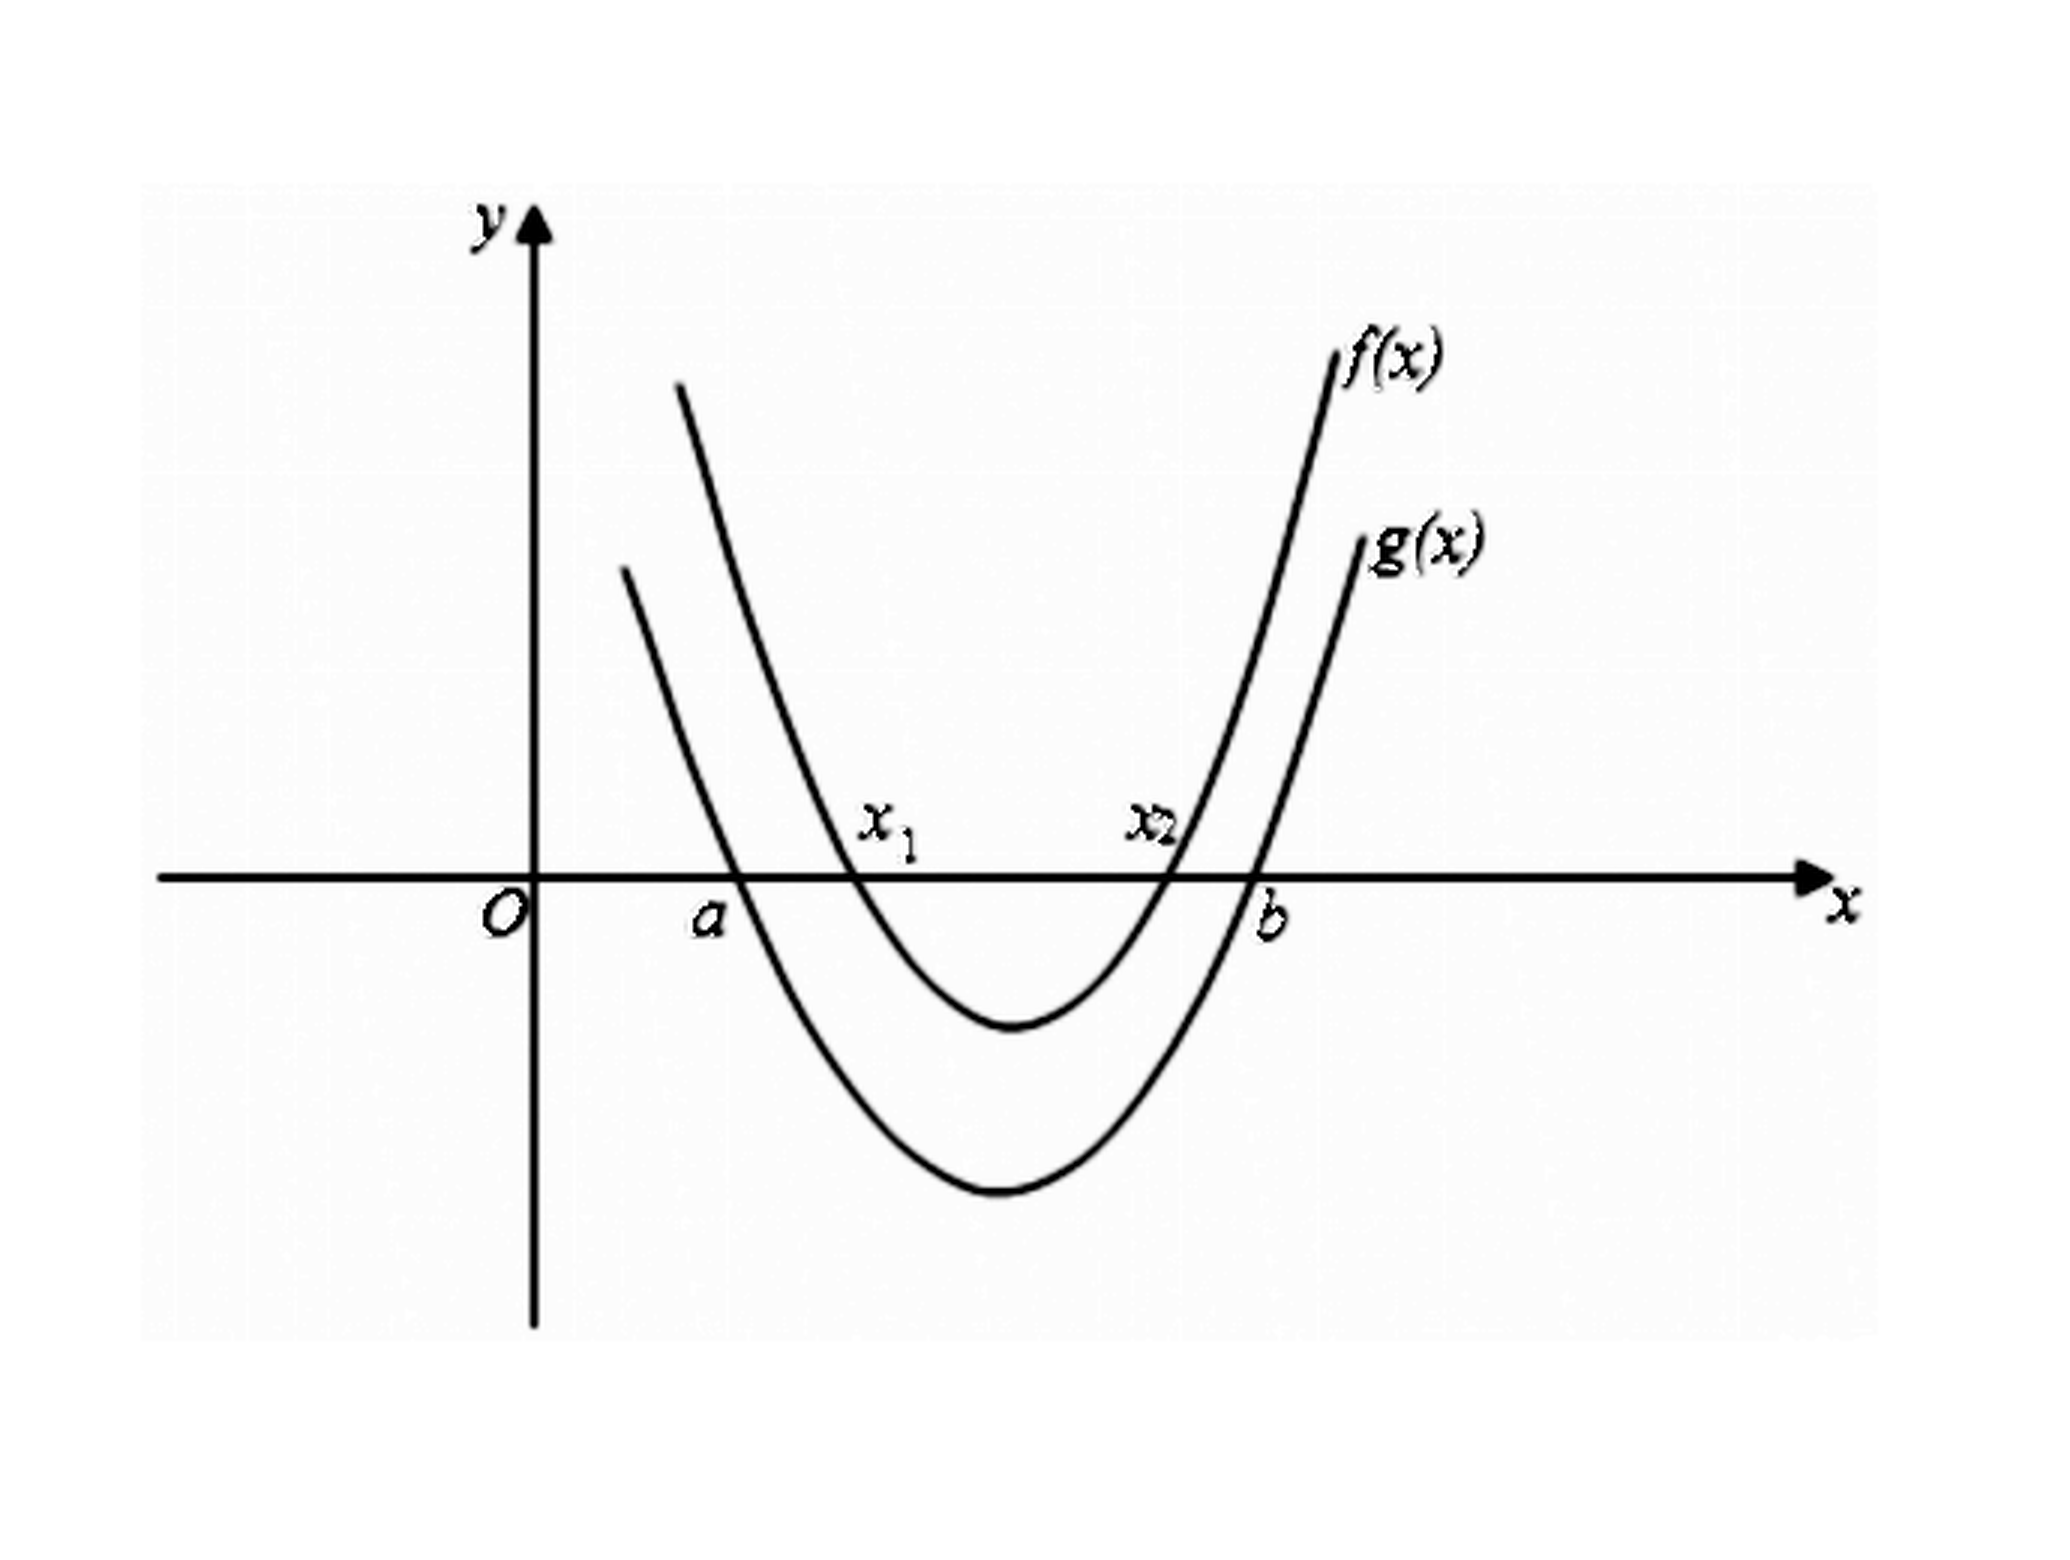
\includegraphics[width=0.52\textwidth]{figures/gao157_q16.png}
\end{center}

\step{由图像得 $a<x_1<x_2<b$，故选 $A$.}
\solend
\fi

\end{enumerate}

\bigsec{三、解答题}

\begin{enumerate}
\setcounter{enumi}{16}

% === Q17 === 解析 6 行；\overline{A}、\varnothing、\subseteq 无、cases
\item 设全集为 $\R$，$m\in\R$，集合 $A=\{x\mid 2<x<5\}$，$B=\{x\mid 2m\leqslant x\leqslant 5m-3\}$.

(1) 若 $m=2$，求 $\overline{A}\cup B$；

(2) 若 $A\cap B=B$，求 $m$ 的取值范围.

\ifanswer
\solbegin
\step{(1) $\overline{A}=\{x\mid x\leqslant2$ 或 $x\geqslant5\}$，当 $m=2$ 时，$B=\{x\mid 4\leqslant x\leqslant7\}$，}
\step{则 $\overline{A}\cup B=\{x\mid x\leqslant2$ 或 $x\geqslant4\}$；}
\step{(2) 因为 $A\cap B=B$，所以 $B$ 是 $A$ 的子集，}
\step{当 $B=\varnothing$ 时，$2m>5m-3$，解得 $m<1$；}
\step{当 $B\ne\varnothing$ 时，$\begin{cases}2m\leqslant5m-3\\2m>2\\5m-3<5\end{cases}$，解得 $1<m<\dfrac85$；}
\step{综上，$m$ 的取值范围是 $(-\infty,1)\cup\left(1,\dfrac85\right)$.}
\solend
\fi

% === Q18 === 解析 2 行；指数式、\lg、换底
\item (1) 设 $a^{2x}=3$，且 $a>0$，求 $\dfrac{a^{3x}+a^{-3x}}{a^x+a^{-x}}$ 的值；

(2) 已知 $\lg2=a, 10^b=3$，用 $a$ 及 $b$ 表示 $\log_{12}25$.

\ifanswer
\solbegin
\step{(1) $\dfrac{a^{3x}+a^{-3x}}{a^x+a^{-x}}=a^{2x}-1+a^{-2x}=3-1+\dfrac13=\dfrac73$；}
\step{(2) $\log_{12}25=\dfrac{\lg25}{\lg12}=\dfrac{2-2\lg2}{2\lg2+\lg3}=\dfrac{2-2a}{2a+b}$.}
\solend
\fi

% === Q19 === 解析 11 行；幂函数、$=0$ 笔误照录、\Delta、\sqrt5、cases
\item 已知幂函数 $f(x)=(m^2+m-1)x^{-2m^2+m+3}$ 在 $(0,+\infty)$ 上为严格增函数.

(1) 求 $f(x)$ 的解析式；

(2) 若 $k+kf(x)>f(x)-x-1$ 对任意实数 $x$ 都成立，求实数 $k$ 的取值范围；

(3) 若关于 $x$ 的不等式 $f(x)\leqslant8x-a$ 的解集中有且仅有 $5$ 个整数，求实数 $a$ 的范围.

\ifanswer
\solbegin
\step{(1) 由题意得 $m^2+m-1=1$，且 $-2m^2+m+3>0$，}
\step{解得 $m=-2$（舍去）或 $m=1$，所以 $f(x)=x^2$；}
\step{(2) $k+kf(x)>f(x)-x-1$ 可化为 $(k-1)x^2+x+k+1=0$ 恒成立，}
\step{当 $k=1$ 时，$x+2>0$，显然不恒成立；}
\step{当 $k\ne1$ 时，要使该二次不等式恒成立，只需 $\begin{cases}k-1>0\\[2pt]\Delta=1-4(k+1)(k-1)\leqslant0\end{cases}$，}
\step{解得 $k\geqslant\dfrac{\sqrt5}{2}$，即所求 $k$ 的范围是 $\left[\dfrac{\sqrt5}{2},+\infty\right)$；}
\step{(3) 不等式 $f(x)\leqslant8x-a$，即 $x^2-8x+a\leqslant0$ 有五个整数解，}
\step{令 $g(x)=x^2-8x+a$，因为该函数开口向上，对称轴为 $x=4$，}
\step{所以解集内的整数为 $2$，$3$，$4$，$5$，$6$，}
\step{由二次函数的性质得，只需 $\begin{cases}g(1)=1-8+a>0\\g(2)=4-8\times2+a\leqslant0\end{cases}$，解得 $7<a\leqslant12$，}
\step{故 $a$ 的取值范围是 $(7,12]$.}
\solend
\fi

% === Q20 === 解析 12 行；材料题、$a+b=1$、大根号、"因出"笔误、分母套分数
\item 问题：正数 $a$、$b$ 满足 $a+b=1$，求 $\dfrac1a+\dfrac2b$ 的最小值.

其中一种解法是：$\dfrac1a+\dfrac2b=\left(\dfrac1a+\dfrac2b\right)(a+b)=1+\dfrac ba+\dfrac{2a}{b}+2\geqslant3+2\sqrt2$，

当且仅当 $\dfrac ba=\dfrac{2a}{b}$ 且 $a+b=1$ 时，即 $a=\sqrt2-1$ 且 $b=2-\sqrt2$ 时取等号.

学习上述解法并解决下列问题：

(1) 若正实数 $x$、$y$ 满足 $x+y=1$，求 $\dfrac2x+\dfrac1y$ 的最小值；

(2) 若实数 $a$、$b$、$x$、$y$ 满足 $\dfrac{x^2}{a^2}-\dfrac{y^2}{b^2}=1$，求证：$a^2-b^2\leqslant(x-y)^2$；

(3) 利用 (2) 的结论，求代数式 $M=\sqrt{2m-5}-\sqrt{m-3}$ 的最小值，并求出使得 $M$ 最小的 $m$ 的值.

\ifanswer
\solbegin
\step{(1) $\dfrac2x+\dfrac1y=(x+y)\left(\dfrac2x+\dfrac1y\right)=3+\dfrac xy+\dfrac{2y}{x}\geqslant3+2\sqrt2$，}
\step{当且仅当 $\dfrac xy=\dfrac{2y}{x}$ 且 $x+y=1$ 时取等号；}
\step{(2) $a^2-b^2=(a^2-b^2)\left(\dfrac{x^2}{a^2}-\dfrac{y^2}{b^2}\right)=x^2+y^2-\left(\dfrac{a^2x^2}{b^2}+\dfrac{b^2y^2}{a^2}\right)$}
\step{$\leqslant x^2+y^2-2\sqrt{\dfrac{a^2x^2}{b^2}\cdot\dfrac{b^2y^2}{a^2}}=x^2+y^2-2xy=(x-y)^2$，}
\step{故当 $b^4x^2=a^4y^2$ 时，等号成立.}
\step{(3) 令 $x=\sqrt{2m-5}, y=\sqrt{m-3}$，由 $\begin{cases}2m-5\geqslant0\\m-3\geqslant0\end{cases}$ 得 $m\geqslant3$，}
\step{$x^2-y^2=(2m-5)-(m-3)=m-2>0$，}
\step{又 $x>0, y>0$，所以 $x>y$，所以 $\dfrac{x^2}{a^2}-\dfrac{y^2}{b^2}=1$，}
\step{由 $x^2-2y^2=1$，得 $\dfrac{x^2}{1}-\dfrac{y^2}{\frac12}=1$，因出 $a^2=1, b^2=\dfrac12$，}
\step{由 (2) 得 $M=\sqrt{2m-5}-\sqrt{m-3}=x-y\geqslant\sqrt{a^2-b^2}=\sqrt{1-\dfrac12}=\dfrac{\sqrt2}{2}$，}
\step{当且仅当 $\dfrac xy=\left(\dfrac ab\right)^2=2$ 取等号，结合 $x^2-2y^2=1$，解得 $x=\sqrt2, y=\dfrac{\sqrt2}{2}$，}
\step{即 $\sqrt{2m-5}=\sqrt2$，得 $m=\dfrac72$，所以 $m=\dfrac72$ 时，$M$ 取得最小值 $\dfrac{\sqrt2}{2}$.}
\solend
\fi

\end{enumerate}

\end{document}
"
% 紧凑版：xelatex "\def\iscompact{1}% 高一157_大境中学_期中.tex
%   —— 高一上数学"2026-2027 年大境中学高一上期中"（试卷版/答案版/紧凑版）
% 试卷版：xelatex 高一157_大境中学_期中.tex
% 答案版：xelatex "\def\isanswer{1}\input{高一157_大境中学_期中.tex}"
% 紧凑版：xelatex "\def\iscompact{1}\input{高一157_大境中学_期中.tex}"
%
% ① 原始材料：微信公众号"魔都数学加油站"文章，连载"27学年高一157"，原文标题
% "27学年高一157——2026-2027年上海市大境中学高一上期中"；
% 原文链接：https://mp.weixin.qq.com/s/s6eDMDVkxc2fcBe8LNm-Tw 。
% 正文为 8 张 PNG 页（01/02/03/04/06 为 4762×6735，05/07/08 为 2560×3620，
% 同一篇各页分辨率混排，逐页按各自分辨率裁图核对）。
% 体例：讲评版——填空 3—12（10 题）、选择 13—16（4 题）、解答 17—20（4 题），
% 共 18 题，自第 3 题起编（1、2 未印在本篇）；末题是第 20 题（不是 21）。
% 除第 4 题只印【答案】外，其余 17 题逐题印【解析】（逐题核实，见 ②）。
% 题目、答案、解析均据原图转录；卷面粉红色水印"魔都数学加油站"及公众号
% 页脚未录入。
% 全卷仅 1 幅配图：第 16 题解析内函数图像（"设 g(x)=(x-a)(x-b)，
% f(x)=g(x)+1，画出函数 g(x) 与函数 f(x) 的图像，如图所示"），
% 解析内配图仅答案版出，裁 figures/gao157_q16.png；逐页通读 8 页确认
% 无题目配图、无表格；08 页下半仅水印、无正文。
%
% 卷首标题：原卷印作"2026-2027 年大境中学高一上期中"，年份区间按全稿惯例排 en dash；
% 原卷卷面未印副标题，本稿按同期中卷知识模块口径补出"集合与常用逻辑用语、不等式、函数"。
%
% ② 与原卷的排版差异：
%   ① 原文从第 3 题起，本稿保留原题号；共 18 题三节，解答题 4 题到 20；
%      三节各自 \begin{enumerate}…\end{enumerate} + \setcounter{enumi}{2/12/16}
%      （题目溯源.py 按 \bigsec 切节、每节独立计 depth，只收 depth==1 的 \item，
%       见 高一156 头注②的订正）；
%   ② 第 4 题只印【答案】、无【解析】，提 \ans{}；其余 17 题逐题印【解析】、
%      逐题设 \solbegin…\solend；四道选择题答案在解析末句"故选 D／D／C／A"
%      （逐个放大复核）、括号 \mbox{（\quad）} 留空；答案版【答案】/【解析】
%      标记数 = 18 = 全卷题数（1 个 \ans ＋ 17 个 \solbegin）；
%   ③ 原卷卷面未印副标题，本稿按知识模块口径补出；
%   ④ 原卷填空横线按全稿惯例排 \blankline[4.4em]；选择题选项段前按惯例各加
%      \keepwithprev；解答题不留作答区、不加 \anspace（原卷为讲评版，109—113 起
%      全稿不用 \anspace）；
%   ⑤ 数集：Q4"$x、y\in R$"、Q6"$x\in R$"、Q10"$a\in Z$"、Q12"$n\in Z$"
%      "$n_1、n_2\in Z$"、Q17"全集为 R／$m\in R$"原卷印斜体 R/Z，按全稿惯例
%      归一 \R／\Z（参见 高一14 头注④、高一150 头注②⑤、高一153 头注⑤）；
%      绝对值排 \lvert…\rvert（Q6 $\lvert x-1\rvert$／$\lvert x+3\rvert$／
%      $\lvert 2x+2\rvert$），集合描述竖线排 \mid（Q12、Q17），空集 \varnothing
%      （Q17"$B=\varnothing$"），补集照原卷上划线排 \overline{A}（Q17），
%      不等号按全稿惯例排 \leqslant／\geqslant；
%   ⑥ 判别式三处（Q8"$\Delta=(-2m)^2-4(m+2)$"、Q15"$\Delta=(a+2)^2+4(a^2-4)<0$"、
%      Q19"$\Delta=1-4(k+1)(k-1)\leqslant0$"）放大比对同形、均为等腰偏高且右斜边
%      加粗的 \Delta，统一照录 \Delta；本卷无扁三角 \triangle 用例（与 高一142／
%      高一151／高一152 的 Δ/△ 混用卷不同）；
%   ⑦ "图像／图象"逐处照录不统一：Q9"图像过点 $(4,2)$""它的图像过点"、
%      Q16"画出函数 $g(x)$ 与函数 $f(x)$ 的图像""由图像得"用"图像"；
%      Q14 题干及解析四处均用"图象"（"的图象关于原点对称""图象关于 $y$ 轴对称"）；
%   ⑧ 原卷笔误／未化简式照录：
%      · Q5 解析"$2\sqrt4+1=5$"根号 4 原卷未化简，照录 \sqrt4；
%      · Q7 解析"$\lg\frac{E_1}{E_2}=\frac25\cdot(m_2-m_1)=\frac25(-1.45+26.7)=10.1$"
%        第一处有 \cdot、第二处无，逐处照录；题干"$m_1-m_2=-\frac52\lg\frac{E_1}{E_2}$"；
%      · Q10 解析"$f(1)=\frac{a+1}{1+2}\geqslant0$"与 cases 第二行分母均印 $1+2$、
%        未化简成 $3$，照录；
%      · Q19 (2)"可化为 $(k-1)x^2+x+k+1=0$ 恒成立"原卷印 $=0$（与 >0 恒成立
%        的题意不符），照录笔误；
%      · Q20 (3)"因出 $a^2=1, b^2=\frac12$"原卷印"因出"（当作"因此"），照录；
%      · Q20 (3)"得 $\frac{x^2}{1}-\frac{y^2}{\frac12}=1$"分母套分数、照录；
%   ⑨ 圈数字①②在文本模式（Q15 解析"①当 $a^2-4=0$ 时""②当 $a^2-4\ne0$ 时"，
%      共 2 枚）；子题标号 (1)(2)(3) 半角括号照录；行末西文句点 ASCII `.`；
%      行中全角逗号／顿号照录；半角逗号在数学组之间是全稿惯例、非笔误
%      （Q8"$x_1+x_2=2m, x_1x_2=m+2$"、Q12"$n\in Z$"、Q18"$\lg2=a, 10^b=3$"、
%      Q20"$a^2=1, b^2=\frac12$"等）；中文弯引号""照录（Q4 命题）；
%   ⑩ 自定义名词：Q11"交叉数"、Q12"$a\otimes b$"新定义运算、Q20"问题／
%      其中一种解法是／学习上述解法并解决下列问题"材料题，均照原卷录入；
%   ⑪ 配图：全卷 1 幅（逐页通读 8 页确认）——Q16 解析内函数图像（05 页右侧，
%      $f(x)$ 与 $g(x)$ 两条抛物线、标注 $a,x_1,x_2,b$），仅答案版出，
%      裁 figures/gao157_q16.png，去粉色水印、去色、3× LANCZOS 放大；
%      图放 \ifanswer 内 \solbegin…\solend 的两 \step 之间（高一108 第 6 题／
%      高一156 Q15 成例）；Q16 题干无"如图"、不需题目配图守卫。
%
% ③ 行数复核：一条 \step = 原卷解析的一个印刷行，cases 块作一个印刷行计；
%    跨半页重叠行（Q5 的"【解析】x-1>0…"、Q10 的"所以 a=-1 或 a=0"、
%    Q12 的"【解析】由 u⊗v…"、Q14 的"f(x)=x² 图象关于 y 轴对称"、
%    Q19 的"(1) 由题意得…"、Q20 的"(3) 令 x=…"等 hi_1/hi_2 两半页共有的行）
%    只计一次，别把原卷折行并起来。
%    逐题数（主会话逐页核对定稿）：Q3：1；Q4：0（只印【答案】、提 \ans{}，
%    不计入 \step 账）；Q5：2；Q6：5；Q7：2；Q8：5；Q9：3；Q10：4；
%    Q11：3；Q12：6；Q13：3；Q14：5；Q15：9；Q16：4；Q17：6；Q18：2；
%    Q19：11；Q20：12。合计 83 条 \step（本卷无 \stepm），与原卷逐题印刷行相等。
%    全卷 18 题：1 题只印【答案】（\ans）、17 题印【解析】（\solbegin…\solend），
%    答案版【答案】/【解析】标记数 = 18 = 全卷题数。
%    全卷除此 6 类外未发现其它笔误／自相矛盾处；17 题印【解析】、1 题印【答案】。
%
\documentclass[a4paper,11pt]{article}
\usepackage{common}

\begin{document}

\examtitlest[3]{2026--2027 年大境中学高一上期中}{集合与常用逻辑用语、不等式、函数}

\bigsec{一、填空题}

\begin{enumerate}
\setcounter{enumi}{2}

% === Q3 === 解析 1 行；$a,b$ 半角逗号照录
\item 若 $a=x^2-2x+1$，$b=x-3$，则 $a,b$ 的大小关系为\blankline[4.4em].

\ifanswer
\solbegin
\step{$a-b=x^2-3x+4=\left(x-\dfrac32\right)^2+\dfrac74>0$，所以 $a>b$.}
\solend
\fi

% === Q4 === 只印【答案】、无【解析】；中文弯引号、\R、顿号；提 \ans{}
\item 用反证法证明命题：“设 $x$、$y\in\R$. 若 $x+y>2$，则 $x>1$ 或 $y>1$”时，假设的内容应该是\blankline[4.4em].

\ifanswer
\ans{$x\leqslant1$ 且 $y\leqslant1$}
\fi

% === Q5 === 解析 2 行；$2\sqrt4+1=5$ 根号 4 未化简照录
\item 当 $x>1$ 时，$x+\dfrac4{x-1}$ 的最小值为\blankline[4.4em].

\ifanswer
\solbegin
\step{$x-1>0$，$x+\dfrac4{x-1}=(x-1)+\dfrac4{x-1}+1\geqslant2\sqrt4+1=5$，}
\step{当且仅当 $x-1=\dfrac4{x-1}$，即 $x=3$ 时取等号，故最小值为 $5$.}
\solend
\fi

% === Q6 === 解析 5 行；绝对值 \lvert…\rvert、\cup、\R
\item 设 $x\in\R$，方程 $\lvert x-1\rvert+\lvert x+3\rvert=\lvert 2x+2\rvert$ 的解集是\blankline[4.4em].

\ifanswer
\solbegin
\step{当 $x\leqslant-3$ 时，方程为 $1-x-x-3=-2x-2$，等式成立；}
\step{当 $-3<x\leqslant-1$ 时，方程为 $1-x+x+3=-2x-2$，解得 $x=-3$，舍去；}
\step{当 $-1<x<1$ 时，方程为 $1-x+x+3=2x+2$，解得 $x=1$，舍去；}
\step{当 $x\geqslant1$ 时，方程为 $x-1+x+3=2x+2$，等式成立，}
\step{综上，方程 $\lvert x-1\rvert+\lvert x+3\rvert=\lvert 2x+2\rvert$ 的解集为 $(-\infty,-3]\cup[1,+\infty)$.}
\solend
\fi

% === Q7 === 解析 2 行；星等材料题、\lg、\cdot 逐处照录、天狼星
\item 在天文学中，天体的明暗程度可以用星等或亮度来描述，两颗星的星等与亮度满足 $m_1-m_2=-\dfrac52\lg\dfrac{E_1}{E_2}$，其中星等为 $m_k$ 的星的亮度为 $E_k(k=1,2)$. 已知太阳的星等为 $-26.7$，天狼星的星等为 $-1.45$，则太阳与天狼星的亮度的比值为\blankline[4.4em].

\ifanswer
\solbegin
\step{两颗星的星等与亮度满足 $m_1-m_2=-\dfrac52\lg\dfrac{E_1}{E_2}$，令 $m_2=-1.45$，$m_1=-26.7$，}
\step{$\lg\dfrac{E_1}{E_2}=\dfrac25\cdot(m_2-m_1)=\dfrac25(-1.45+26.7)=10.1$，$\dfrac{E_1}{E_2}=10^{10.1}$.}
\solend
\fi

% === Q8 === 解析 5 行；韦达定理、判别式 \Delta、半角逗号在数学组间
\item 已知方程 $x^2-2mx+m+2=0$ 有两个实数根 $x_1,x_2$，满足 $x_1^2+x_2^2=2$，则实数 $m$ 的值为\blankline[4.4em].

\ifanswer
\solbegin
\step{对于方程 $x^2-2mx+m+2=0$，由韦达定理得 $x_1+x_2=2m, x_1x_2=m+2$，}
\step{又 $x_1^2+x_2^2=(x_1+x_2)^2-2x_1x_2=(2m)^2-2(m+2)=4m^2-2m-4=2$，}
\step{解得 $m=\dfrac32$ 或 $m=-1$，}
\step{因为方程有两个实数根，所以 $\Delta=(-2m)^2-4(m+2)=4m^2-4m-8\geqslant0$，}
\step{解得 $m\leqslant-1$ 或 $m\geqslant2$，故 $m=-1$.}
\solend
\fi

% === Q9 === 解析 3 行；"图像"照录、$x^\alpha$、$x^{1/2}=\sqrt{x}$
\item 已知幂函数 $y=f(x)$ 的图像过点 $(4,2)$，则不等式 $f(x^2-2x)<f(2-x)$ 的解集为\blankline[4.4em].

\ifanswer
\solbegin
\step{设幂函数 $y=f(x)=x^\alpha$，它的图像过点 $(4,2)$，所以 $4^\alpha=2$，$\alpha=\dfrac12$，}
\step{故 $f(x)=x^{\frac12}=\sqrt{x}$，由不等式 $f(x^2-2x)<f(2-x)$，}
\step{得 $0\leqslant x^2-2x<2-x$，得 $-1<x\leqslant0$，故解集为 $(-1,0]$.}
\solend
\fi

% === Q10 === 解析 4 行；$a\in\Z$、cases（分母 $1+2$ 未化简）、参数分离
\item 已知函数 $y=\dfrac{ax+1}{x+2}$（常数 $a\in\Z$）. 要使该函数在区间 $[1,+\infty)$ 上是严格减函数，并且函数值不恒为负，则满足条件的 $a$ 的取值为\blankline[4.4em].

\ifanswer
\solbegin
\step{函数参数分离为 $y=\dfrac{a(x+2)+1-2a}{x+2}=a+\dfrac{1-2a}{x+2}$，}
\step{若函数在区间 $[1,+\infty)$ 上严格减函数，则 $1-2a>0$，}
\step{且函数的最大值 $f(1)=\dfrac{a+1}{1+2}\geqslant0$，即 $\begin{cases}1-2a>0\\[2pt]\dfrac{a+1}{1+2}\geqslant0\end{cases}$，解得 $-1\leqslant a<\dfrac12$，又 $a\in\Z$，}
\step{所以 $a=-1$ 或 $a=0$.}
\solend
\fi

% === Q11 === 解析 3 行；"交叉数"自定义名词、$(-1)^t$、$2^5$、$32\times3=96$
\item 对非空集合 $A$ 中的每个元素 $t$，都乘以 $(-1)^t$ 再求和，称为集合 $A$ 的交叉数，例如 $A=\{2,3,6\}$，则集合 $A$ 的交叉数为 $(-1)^2\cdot2+(-1)^3\cdot3+(-1)^6\cdot6=5$. 若集合 $W=\{1,2,3,4,5,6\}$，则 $W$ 的所有非空子集的交叉数的总和为\blankline[4.4em].

\ifanswer
\solbegin
\step{固定 $W$ 中的任一元素，其余 $5$ 个元素各有选或不选两种情况，}
\step{因此该元素出现在 $2^5$ 个非空子集中，}
\step{所有交叉数的总和为 $2^5(-1+2-3+4-5+6)=32\times3=96$.}
\solend
\fi

% === Q12 === 解析 6 行；\otimes、\lambda、\mid、\Z、\times 与 \cdot 逐处照录
\item 对于任意两个正实数 $a$、$b$，定义 $a\otimes b=\lambda\cdot\dfrac ab$，其中常数 $\lambda\in\left(\dfrac{\sqrt2}{2},1\right)$. 若 $u\geqslant v>0$，且 $u\otimes v$ 与 $v\otimes u$ 都是集合 $\left\{x\mid x=\dfrac n2,n\in\Z\right\}$ 的元素，则 $u\otimes v=$\blankline[4.4em].

\ifanswer
\solbegin
\step{由 $u\otimes v$ 与 $v\otimes u$ 都是集合 $\left\{x\mid x=\dfrac n2,n\in\Z\right\}$ 的元素，}
\step{不妨设 $\lambda\times\dfrac uv=\dfrac12 n_1$，$\lambda\times\dfrac vu=\dfrac12 n_2$，$n_1$、$n_2\in\Z$，}
\step{因为 $u\geqslant v>0$，所以 $0<\dfrac vu\leqslant1$，因为 $\lambda\in\left(\dfrac{\sqrt2}{2},1\right)$，所以 $\dfrac12 n_2=\lambda\cdot\dfrac vu\in(0,1)$，}
\step{因为 $n_2\in\Z$，所以 $n_2=1$，即 $\dfrac12=\dfrac{\lambda v}{u}$，所以 $\lambda=\dfrac{u}{2v}\in\left(\dfrac{\sqrt2}{2},1\right)$，}
\step{所以 $\dfrac uv\in(\sqrt2,2)$，$\dfrac{u^2}{v^2}\in(2,4)$，则 $\lambda\cdot\dfrac uv=\dfrac{u^2}{v^2}\times\dfrac12=\dfrac12 n_1\in(1,2)$，}
\step{因为 $n_1\in\Z$，所以 $n_1=3$，$\dfrac12 n_1=\dfrac32$，故 $u\otimes v=\dfrac32$.}
\solend
\fi

\end{enumerate}

\bigsec{二、选择题}

\begin{enumerate}
\setcounter{enumi}{12}

% === Q13 === 解析 3 行；选项段 \keepwithprev；故选 D
\item 下列不等式成立的为\mbox{（\quad）}

\keepwithprev
A. 若 $a>b$，则 $ac^2>bc^2$\qquad B. 若 $a>b$，则 $a^2>b^2$

C. 若 $a>b$，$c>d$，则 $a+b>c+d$\qquad D. 若 $a>b$，则 $a^3>b^3$

\ifanswer
\solbegin
\step{A 中 $c=0$ 时不成立；B 取 $a=1$，$b=-2$ 不成立；}
\step{C 取 $a=1$，$b=0$，$c=5$，$d=0$ 不成立.}
\step{幂函数 $y=x^3$ 在实数集上严格递增，所以 $a>b\Rightarrow a^3>b^3$，故选 $D$.}
\solend
\fi

% === Q14 === 解析 5 行；"图象"四处照录；故选 D
\item 幂函数 $f(x)=x^\alpha$ 的图象关于原点对称，且在 $(-\infty,0)$ 上是严格增函数，则 $f(x)$ 可以是\mbox{（\quad）}

\keepwithprev
A. $f(x)=x^{-1}$\qquad B. $f(x)=x^{\frac12}$\qquad C. $f(x)=x^2$\qquad D. $f(x)=x^3$

\ifanswer
\solbegin
\step{$f(x)=\dfrac1x$ 的图象关于原点对称，在 $(-\infty,0)$ 上是严格减函数，故 $A$ 错误；}
\step{$f(x)=x^{\frac12}$ 在 $(-\infty,0)$ 上无意义，故 $B$ 错误；}
\step{$f(x)=x^2$ 图象关于 $y$ 轴对称，故 $C$ 错误；}
\step{$f(x)=x^3$ 的图象关于原点对称，且在 $(-\infty,0)$ 上是严格增函数，故 $D$ 正确.}
\step{故选 $D$.}
\solend
\fi

% === Q15 === 解析 9 行；圈数字①②、\Delta、cases；故选 C
\item 若关于 $x$ 的不等式 $(a^2-4)x^2+(a+2)x-1\geqslant0$ 的解集不为空集，则实数 $a$ 的取值范围为\mbox{（\quad）}

\keepwithprev
A. $\left(-2,\dfrac65\right]$\qquad B. $\left[-2,\dfrac65\right]$

C. $(-\infty,-2)\cup\left[\dfrac65,+\infty\right)$\qquad D. $(-\infty,-2]\cup\left[\dfrac65,+\infty\right)$

\ifanswer
\solbegin
\step{①当 $a^2-4=0$ 时，$a=\pm2$，}
\step{若 $a=2$ 时，原不等式为 $4x-1\geqslant0$，则不等式的解集不是空集；}
\step{若 $a=-2$ 时，原不等式为 $-1\geqslant0$，无解，不符合题意；}
\step{②当 $a^2-4\ne0$ 时，$a\ne\pm2$，}
\step{若 $(a^2-4)x^2+(a+2)x-1\geqslant0$ 的解集是空集，则 $\begin{cases}a^2-4<0\\[2pt]\Delta=(a+2)^2+4(a^2-4)<0\end{cases}$，}
\step{解得 $-2<a<\dfrac65$，}
\step{则当不等式 $(a^2-4)x^2+(a+2)x-1\geqslant0$ 的解集不为空集时，}
\step{有 $a<-2$ 或 $a\geqslant\dfrac65$ 且 $a\ne2$，}
\step{综上，实数 $a$ 的取值范围为 $(-\infty,-2)\cup\left[\dfrac65,+\infty\right)$，故选 $C$.}
\solend
\fi

% === Q16 === 解析 4 行＋1 幅解析内配图（仅答案版）；"图像"照录；故选 A
\item 已知实数 $a<b$，关于 $x$ 的不等式 $x^2-(a+b)x+ab+1<0$ 的解集为 $(x_1,x_2)$，则实数 $a$、$b$、$x_1$、$x_2$ 从小到大的排列是\mbox{（\quad）}

\keepwithprev
A. $a<x_1<x_2<b$\qquad B. $x_1<a<b<x_2$\qquad C. $a<x_1<b<x_2$\qquad D. $x_1<a<x_2<b$

\ifanswer
\solbegin
\step{不等式 $x^2-(a+b)x+ab+1<0$ 可化为 $(x-a)(x-b)+1<0$，}
\step{设 $g(x)=(x-a)(x-b)$，$f(x)=g(x)+1$，}
\step{画出函数 $g(x)$ 与函数 $f(x)$ 的图像，如图所示，}

\begin{center}
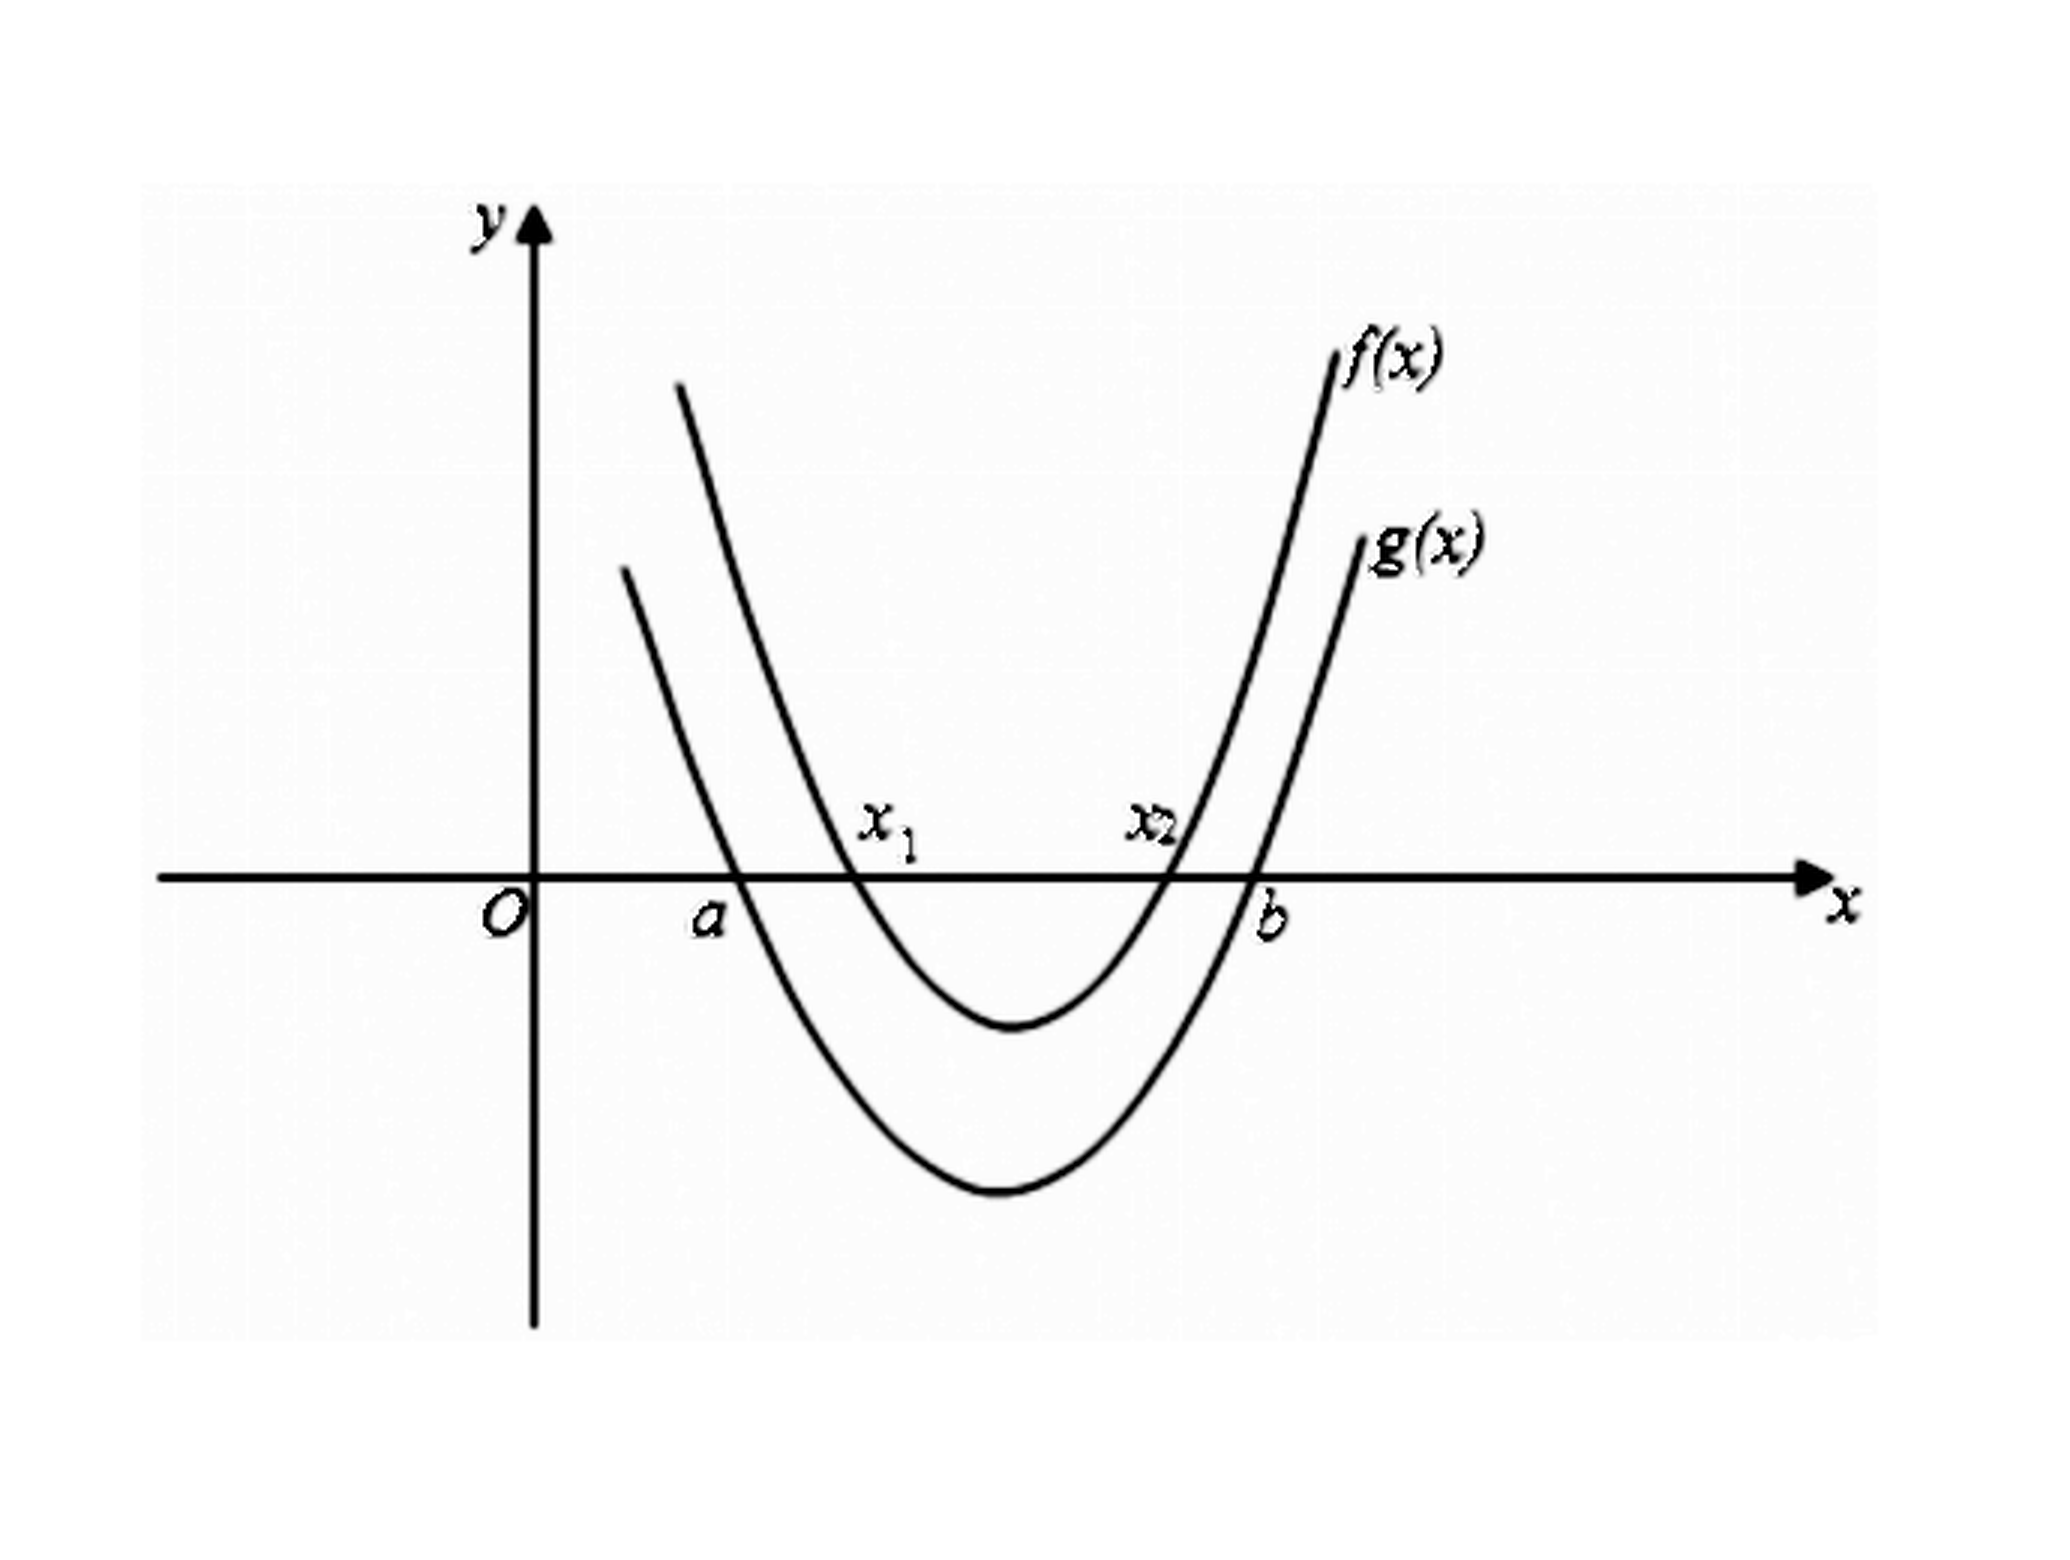
\includegraphics[width=0.52\textwidth]{figures/gao157_q16.png}
\end{center}

\step{由图像得 $a<x_1<x_2<b$，故选 $A$.}
\solend
\fi

\end{enumerate}

\bigsec{三、解答题}

\begin{enumerate}
\setcounter{enumi}{16}

% === Q17 === 解析 6 行；\overline{A}、\varnothing、\subseteq 无、cases
\item 设全集为 $\R$，$m\in\R$，集合 $A=\{x\mid 2<x<5\}$，$B=\{x\mid 2m\leqslant x\leqslant 5m-3\}$.

(1) 若 $m=2$，求 $\overline{A}\cup B$；

(2) 若 $A\cap B=B$，求 $m$ 的取值范围.

\ifanswer
\solbegin
\step{(1) $\overline{A}=\{x\mid x\leqslant2$ 或 $x\geqslant5\}$，当 $m=2$ 时，$B=\{x\mid 4\leqslant x\leqslant7\}$，}
\step{则 $\overline{A}\cup B=\{x\mid x\leqslant2$ 或 $x\geqslant4\}$；}
\step{(2) 因为 $A\cap B=B$，所以 $B$ 是 $A$ 的子集，}
\step{当 $B=\varnothing$ 时，$2m>5m-3$，解得 $m<1$；}
\step{当 $B\ne\varnothing$ 时，$\begin{cases}2m\leqslant5m-3\\2m>2\\5m-3<5\end{cases}$，解得 $1<m<\dfrac85$；}
\step{综上，$m$ 的取值范围是 $(-\infty,1)\cup\left(1,\dfrac85\right)$.}
\solend
\fi

% === Q18 === 解析 2 行；指数式、\lg、换底
\item (1) 设 $a^{2x}=3$，且 $a>0$，求 $\dfrac{a^{3x}+a^{-3x}}{a^x+a^{-x}}$ 的值；

(2) 已知 $\lg2=a, 10^b=3$，用 $a$ 及 $b$ 表示 $\log_{12}25$.

\ifanswer
\solbegin
\step{(1) $\dfrac{a^{3x}+a^{-3x}}{a^x+a^{-x}}=a^{2x}-1+a^{-2x}=3-1+\dfrac13=\dfrac73$；}
\step{(2) $\log_{12}25=\dfrac{\lg25}{\lg12}=\dfrac{2-2\lg2}{2\lg2+\lg3}=\dfrac{2-2a}{2a+b}$.}
\solend
\fi

% === Q19 === 解析 11 行；幂函数、$=0$ 笔误照录、\Delta、\sqrt5、cases
\item 已知幂函数 $f(x)=(m^2+m-1)x^{-2m^2+m+3}$ 在 $(0,+\infty)$ 上为严格增函数.

(1) 求 $f(x)$ 的解析式；

(2) 若 $k+kf(x)>f(x)-x-1$ 对任意实数 $x$ 都成立，求实数 $k$ 的取值范围；

(3) 若关于 $x$ 的不等式 $f(x)\leqslant8x-a$ 的解集中有且仅有 $5$ 个整数，求实数 $a$ 的范围.

\ifanswer
\solbegin
\step{(1) 由题意得 $m^2+m-1=1$，且 $-2m^2+m+3>0$，}
\step{解得 $m=-2$（舍去）或 $m=1$，所以 $f(x)=x^2$；}
\step{(2) $k+kf(x)>f(x)-x-1$ 可化为 $(k-1)x^2+x+k+1=0$ 恒成立，}
\step{当 $k=1$ 时，$x+2>0$，显然不恒成立；}
\step{当 $k\ne1$ 时，要使该二次不等式恒成立，只需 $\begin{cases}k-1>0\\[2pt]\Delta=1-4(k+1)(k-1)\leqslant0\end{cases}$，}
\step{解得 $k\geqslant\dfrac{\sqrt5}{2}$，即所求 $k$ 的范围是 $\left[\dfrac{\sqrt5}{2},+\infty\right)$；}
\step{(3) 不等式 $f(x)\leqslant8x-a$，即 $x^2-8x+a\leqslant0$ 有五个整数解，}
\step{令 $g(x)=x^2-8x+a$，因为该函数开口向上，对称轴为 $x=4$，}
\step{所以解集内的整数为 $2$，$3$，$4$，$5$，$6$，}
\step{由二次函数的性质得，只需 $\begin{cases}g(1)=1-8+a>0\\g(2)=4-8\times2+a\leqslant0\end{cases}$，解得 $7<a\leqslant12$，}
\step{故 $a$ 的取值范围是 $(7,12]$.}
\solend
\fi

% === Q20 === 解析 12 行；材料题、$a+b=1$、大根号、"因出"笔误、分母套分数
\item 问题：正数 $a$、$b$ 满足 $a+b=1$，求 $\dfrac1a+\dfrac2b$ 的最小值.

其中一种解法是：$\dfrac1a+\dfrac2b=\left(\dfrac1a+\dfrac2b\right)(a+b)=1+\dfrac ba+\dfrac{2a}{b}+2\geqslant3+2\sqrt2$，

当且仅当 $\dfrac ba=\dfrac{2a}{b}$ 且 $a+b=1$ 时，即 $a=\sqrt2-1$ 且 $b=2-\sqrt2$ 时取等号.

学习上述解法并解决下列问题：

(1) 若正实数 $x$、$y$ 满足 $x+y=1$，求 $\dfrac2x+\dfrac1y$ 的最小值；

(2) 若实数 $a$、$b$、$x$、$y$ 满足 $\dfrac{x^2}{a^2}-\dfrac{y^2}{b^2}=1$，求证：$a^2-b^2\leqslant(x-y)^2$；

(3) 利用 (2) 的结论，求代数式 $M=\sqrt{2m-5}-\sqrt{m-3}$ 的最小值，并求出使得 $M$ 最小的 $m$ 的值.

\ifanswer
\solbegin
\step{(1) $\dfrac2x+\dfrac1y=(x+y)\left(\dfrac2x+\dfrac1y\right)=3+\dfrac xy+\dfrac{2y}{x}\geqslant3+2\sqrt2$，}
\step{当且仅当 $\dfrac xy=\dfrac{2y}{x}$ 且 $x+y=1$ 时取等号；}
\step{(2) $a^2-b^2=(a^2-b^2)\left(\dfrac{x^2}{a^2}-\dfrac{y^2}{b^2}\right)=x^2+y^2-\left(\dfrac{a^2x^2}{b^2}+\dfrac{b^2y^2}{a^2}\right)$}
\step{$\leqslant x^2+y^2-2\sqrt{\dfrac{a^2x^2}{b^2}\cdot\dfrac{b^2y^2}{a^2}}=x^2+y^2-2xy=(x-y)^2$，}
\step{故当 $b^4x^2=a^4y^2$ 时，等号成立.}
\step{(3) 令 $x=\sqrt{2m-5}, y=\sqrt{m-3}$，由 $\begin{cases}2m-5\geqslant0\\m-3\geqslant0\end{cases}$ 得 $m\geqslant3$，}
\step{$x^2-y^2=(2m-5)-(m-3)=m-2>0$，}
\step{又 $x>0, y>0$，所以 $x>y$，所以 $\dfrac{x^2}{a^2}-\dfrac{y^2}{b^2}=1$，}
\step{由 $x^2-2y^2=1$，得 $\dfrac{x^2}{1}-\dfrac{y^2}{\frac12}=1$，因出 $a^2=1, b^2=\dfrac12$，}
\step{由 (2) 得 $M=\sqrt{2m-5}-\sqrt{m-3}=x-y\geqslant\sqrt{a^2-b^2}=\sqrt{1-\dfrac12}=\dfrac{\sqrt2}{2}$，}
\step{当且仅当 $\dfrac xy=\left(\dfrac ab\right)^2=2$ 取等号，结合 $x^2-2y^2=1$，解得 $x=\sqrt2, y=\dfrac{\sqrt2}{2}$，}
\step{即 $\sqrt{2m-5}=\sqrt2$，得 $m=\dfrac72$，所以 $m=\dfrac72$ 时，$M$ 取得最小值 $\dfrac{\sqrt2}{2}$.}
\solend
\fi

\end{enumerate}

\end{document}
"
%
% ① 原始材料：微信公众号"魔都数学加油站"文章，连载"27学年高一157"，原文标题
% "27学年高一157——2026-2027年上海市大境中学高一上期中"；
% 原文链接：https://mp.weixin.qq.com/s/s6eDMDVkxc2fcBe8LNm-Tw 。
% 正文为 8 张 PNG 页（01/02/03/04/06 为 4762×6735，05/07/08 为 2560×3620，
% 同一篇各页分辨率混排，逐页按各自分辨率裁图核对）。
% 体例：讲评版——填空 3—12（10 题）、选择 13—16（4 题）、解答 17—20（4 题），
% 共 18 题，自第 3 题起编（1、2 未印在本篇）；末题是第 20 题（不是 21）。
% 除第 4 题只印【答案】外，其余 17 题逐题印【解析】（逐题核实，见 ②）。
% 题目、答案、解析均据原图转录；卷面粉红色水印"魔都数学加油站"及公众号
% 页脚未录入。
% 全卷仅 1 幅配图：第 16 题解析内函数图像（"设 g(x)=(x-a)(x-b)，
% f(x)=g(x)+1，画出函数 g(x) 与函数 f(x) 的图像，如图所示"），
% 解析内配图仅答案版出，裁 figures/gao157_q16.png；逐页通读 8 页确认
% 无题目配图、无表格；08 页下半仅水印、无正文。
%
% 卷首标题：原卷印作"2026-2027 年大境中学高一上期中"，年份区间按全稿惯例排 en dash；
% 原卷卷面未印副标题，本稿按同期中卷知识模块口径补出"集合与常用逻辑用语、不等式、函数"。
%
% ② 与原卷的排版差异：
%   ① 原文从第 3 题起，本稿保留原题号；共 18 题三节，解答题 4 题到 20；
%      三节各自 \begin{enumerate}…\end{enumerate} + \setcounter{enumi}{2/12/16}
%      （题目溯源.py 按 \bigsec 切节、每节独立计 depth，只收 depth==1 的 \item，
%       见 高一156 头注②的订正）；
%   ② 第 4 题只印【答案】、无【解析】，提 \ans{}；其余 17 题逐题印【解析】、
%      逐题设 \solbegin…\solend；四道选择题答案在解析末句"故选 D／D／C／A"
%      （逐个放大复核）、括号 \mbox{（\quad）} 留空；答案版【答案】/【解析】
%      标记数 = 18 = 全卷题数（1 个 \ans ＋ 17 个 \solbegin）；
%   ③ 原卷卷面未印副标题，本稿按知识模块口径补出；
%   ④ 原卷填空横线按全稿惯例排 \blankline[4.4em]；选择题选项段前按惯例各加
%      \keepwithprev；解答题不留作答区、不加 \anspace（原卷为讲评版，109—113 起
%      全稿不用 \anspace）；
%   ⑤ 数集：Q4"$x、y\in R$"、Q6"$x\in R$"、Q10"$a\in Z$"、Q12"$n\in Z$"
%      "$n_1、n_2\in Z$"、Q17"全集为 R／$m\in R$"原卷印斜体 R/Z，按全稿惯例
%      归一 \R／\Z（参见 高一14 头注④、高一150 头注②⑤、高一153 头注⑤）；
%      绝对值排 \lvert…\rvert（Q6 $\lvert x-1\rvert$／$\lvert x+3\rvert$／
%      $\lvert 2x+2\rvert$），集合描述竖线排 \mid（Q12、Q17），空集 \varnothing
%      （Q17"$B=\varnothing$"），补集照原卷上划线排 \overline{A}（Q17），
%      不等号按全稿惯例排 \leqslant／\geqslant；
%   ⑥ 判别式三处（Q8"$\Delta=(-2m)^2-4(m+2)$"、Q15"$\Delta=(a+2)^2+4(a^2-4)<0$"、
%      Q19"$\Delta=1-4(k+1)(k-1)\leqslant0$"）放大比对同形、均为等腰偏高且右斜边
%      加粗的 \Delta，统一照录 \Delta；本卷无扁三角 \triangle 用例（与 高一142／
%      高一151／高一152 的 Δ/△ 混用卷不同）；
%   ⑦ "图像／图象"逐处照录不统一：Q9"图像过点 $(4,2)$""它的图像过点"、
%      Q16"画出函数 $g(x)$ 与函数 $f(x)$ 的图像""由图像得"用"图像"；
%      Q14 题干及解析四处均用"图象"（"的图象关于原点对称""图象关于 $y$ 轴对称"）；
%   ⑧ 原卷笔误／未化简式照录：
%      · Q5 解析"$2\sqrt4+1=5$"根号 4 原卷未化简，照录 \sqrt4；
%      · Q7 解析"$\lg\frac{E_1}{E_2}=\frac25\cdot(m_2-m_1)=\frac25(-1.45+26.7)=10.1$"
%        第一处有 \cdot、第二处无，逐处照录；题干"$m_1-m_2=-\frac52\lg\frac{E_1}{E_2}$"；
%      · Q10 解析"$f(1)=\frac{a+1}{1+2}\geqslant0$"与 cases 第二行分母均印 $1+2$、
%        未化简成 $3$，照录；
%      · Q19 (2)"可化为 $(k-1)x^2+x+k+1=0$ 恒成立"原卷印 $=0$（与 >0 恒成立
%        的题意不符），照录笔误；
%      · Q20 (3)"因出 $a^2=1, b^2=\frac12$"原卷印"因出"（当作"因此"），照录；
%      · Q20 (3)"得 $\frac{x^2}{1}-\frac{y^2}{\frac12}=1$"分母套分数、照录；
%   ⑨ 圈数字①②在文本模式（Q15 解析"①当 $a^2-4=0$ 时""②当 $a^2-4\ne0$ 时"，
%      共 2 枚）；子题标号 (1)(2)(3) 半角括号照录；行末西文句点 ASCII `.`；
%      行中全角逗号／顿号照录；半角逗号在数学组之间是全稿惯例、非笔误
%      （Q8"$x_1+x_2=2m, x_1x_2=m+2$"、Q12"$n\in Z$"、Q18"$\lg2=a, 10^b=3$"、
%      Q20"$a^2=1, b^2=\frac12$"等）；中文弯引号""照录（Q4 命题）；
%   ⑩ 自定义名词：Q11"交叉数"、Q12"$a\otimes b$"新定义运算、Q20"问题／
%      其中一种解法是／学习上述解法并解决下列问题"材料题，均照原卷录入；
%   ⑪ 配图：全卷 1 幅（逐页通读 8 页确认）——Q16 解析内函数图像（05 页右侧，
%      $f(x)$ 与 $g(x)$ 两条抛物线、标注 $a,x_1,x_2,b$），仅答案版出，
%      裁 figures/gao157_q16.png，去粉色水印、去色、3× LANCZOS 放大；
%      图放 \ifanswer 内 \solbegin…\solend 的两 \step 之间（高一108 第 6 题／
%      高一156 Q15 成例）；Q16 题干无"如图"、不需题目配图守卫。
%
% ③ 行数复核：一条 \step = 原卷解析的一个印刷行，cases 块作一个印刷行计；
%    跨半页重叠行（Q5 的"【解析】x-1>0…"、Q10 的"所以 a=-1 或 a=0"、
%    Q12 的"【解析】由 u⊗v…"、Q14 的"f(x)=x² 图象关于 y 轴对称"、
%    Q19 的"(1) 由题意得…"、Q20 的"(3) 令 x=…"等 hi_1/hi_2 两半页共有的行）
%    只计一次，别把原卷折行并起来。
%    逐题数（主会话逐页核对定稿）：Q3：1；Q4：0（只印【答案】、提 \ans{}，
%    不计入 \step 账）；Q5：2；Q6：5；Q7：2；Q8：5；Q9：3；Q10：4；
%    Q11：3；Q12：6；Q13：3；Q14：5；Q15：9；Q16：4；Q17：6；Q18：2；
%    Q19：11；Q20：12。合计 83 条 \step（本卷无 \stepm），与原卷逐题印刷行相等。
%    全卷 18 题：1 题只印【答案】（\ans）、17 题印【解析】（\solbegin…\solend），
%    答案版【答案】/【解析】标记数 = 18 = 全卷题数。
%    全卷除此 6 类外未发现其它笔误／自相矛盾处；17 题印【解析】、1 题印【答案】。
%
\documentclass[a4paper,11pt]{article}
\usepackage{common}

\begin{document}

\examtitlest[3]{2026--2027 年大境中学高一上期中}{集合与常用逻辑用语、不等式、函数}

\bigsec{一、填空题}

\begin{enumerate}
\setcounter{enumi}{2}

% === Q3 === 解析 1 行；$a,b$ 半角逗号照录
\item 若 $a=x^2-2x+1$，$b=x-3$，则 $a,b$ 的大小关系为\blankline[4.4em].

\ifanswer
\solbegin
\step{$a-b=x^2-3x+4=\left(x-\dfrac32\right)^2+\dfrac74>0$，所以 $a>b$.}
\solend
\fi

% === Q4 === 只印【答案】、无【解析】；中文弯引号、\R、顿号；提 \ans{}
\item 用反证法证明命题：“设 $x$、$y\in\R$. 若 $x+y>2$，则 $x>1$ 或 $y>1$”时，假设的内容应该是\blankline[4.4em].

\ifanswer
\ans{$x\leqslant1$ 且 $y\leqslant1$}
\fi

% === Q5 === 解析 2 行；$2\sqrt4+1=5$ 根号 4 未化简照录
\item 当 $x>1$ 时，$x+\dfrac4{x-1}$ 的最小值为\blankline[4.4em].

\ifanswer
\solbegin
\step{$x-1>0$，$x+\dfrac4{x-1}=(x-1)+\dfrac4{x-1}+1\geqslant2\sqrt4+1=5$，}
\step{当且仅当 $x-1=\dfrac4{x-1}$，即 $x=3$ 时取等号，故最小值为 $5$.}
\solend
\fi

% === Q6 === 解析 5 行；绝对值 \lvert…\rvert、\cup、\R
\item 设 $x\in\R$，方程 $\lvert x-1\rvert+\lvert x+3\rvert=\lvert 2x+2\rvert$ 的解集是\blankline[4.4em].

\ifanswer
\solbegin
\step{当 $x\leqslant-3$ 时，方程为 $1-x-x-3=-2x-2$，等式成立；}
\step{当 $-3<x\leqslant-1$ 时，方程为 $1-x+x+3=-2x-2$，解得 $x=-3$，舍去；}
\step{当 $-1<x<1$ 时，方程为 $1-x+x+3=2x+2$，解得 $x=1$，舍去；}
\step{当 $x\geqslant1$ 时，方程为 $x-1+x+3=2x+2$，等式成立，}
\step{综上，方程 $\lvert x-1\rvert+\lvert x+3\rvert=\lvert 2x+2\rvert$ 的解集为 $(-\infty,-3]\cup[1,+\infty)$.}
\solend
\fi

% === Q7 === 解析 2 行；星等材料题、\lg、\cdot 逐处照录、天狼星
\item 在天文学中，天体的明暗程度可以用星等或亮度来描述，两颗星的星等与亮度满足 $m_1-m_2=-\dfrac52\lg\dfrac{E_1}{E_2}$，其中星等为 $m_k$ 的星的亮度为 $E_k(k=1,2)$. 已知太阳的星等为 $-26.7$，天狼星的星等为 $-1.45$，则太阳与天狼星的亮度的比值为\blankline[4.4em].

\ifanswer
\solbegin
\step{两颗星的星等与亮度满足 $m_1-m_2=-\dfrac52\lg\dfrac{E_1}{E_2}$，令 $m_2=-1.45$，$m_1=-26.7$，}
\step{$\lg\dfrac{E_1}{E_2}=\dfrac25\cdot(m_2-m_1)=\dfrac25(-1.45+26.7)=10.1$，$\dfrac{E_1}{E_2}=10^{10.1}$.}
\solend
\fi

% === Q8 === 解析 5 行；韦达定理、判别式 \Delta、半角逗号在数学组间
\item 已知方程 $x^2-2mx+m+2=0$ 有两个实数根 $x_1,x_2$，满足 $x_1^2+x_2^2=2$，则实数 $m$ 的值为\blankline[4.4em].

\ifanswer
\solbegin
\step{对于方程 $x^2-2mx+m+2=0$，由韦达定理得 $x_1+x_2=2m, x_1x_2=m+2$，}
\step{又 $x_1^2+x_2^2=(x_1+x_2)^2-2x_1x_2=(2m)^2-2(m+2)=4m^2-2m-4=2$，}
\step{解得 $m=\dfrac32$ 或 $m=-1$，}
\step{因为方程有两个实数根，所以 $\Delta=(-2m)^2-4(m+2)=4m^2-4m-8\geqslant0$，}
\step{解得 $m\leqslant-1$ 或 $m\geqslant2$，故 $m=-1$.}
\solend
\fi

% === Q9 === 解析 3 行；"图像"照录、$x^\alpha$、$x^{1/2}=\sqrt{x}$
\item 已知幂函数 $y=f(x)$ 的图像过点 $(4,2)$，则不等式 $f(x^2-2x)<f(2-x)$ 的解集为\blankline[4.4em].

\ifanswer
\solbegin
\step{设幂函数 $y=f(x)=x^\alpha$，它的图像过点 $(4,2)$，所以 $4^\alpha=2$，$\alpha=\dfrac12$，}
\step{故 $f(x)=x^{\frac12}=\sqrt{x}$，由不等式 $f(x^2-2x)<f(2-x)$，}
\step{得 $0\leqslant x^2-2x<2-x$，得 $-1<x\leqslant0$，故解集为 $(-1,0]$.}
\solend
\fi

% === Q10 === 解析 4 行；$a\in\Z$、cases（分母 $1+2$ 未化简）、参数分离
\item 已知函数 $y=\dfrac{ax+1}{x+2}$（常数 $a\in\Z$）. 要使该函数在区间 $[1,+\infty)$ 上是严格减函数，并且函数值不恒为负，则满足条件的 $a$ 的取值为\blankline[4.4em].

\ifanswer
\solbegin
\step{函数参数分离为 $y=\dfrac{a(x+2)+1-2a}{x+2}=a+\dfrac{1-2a}{x+2}$，}
\step{若函数在区间 $[1,+\infty)$ 上严格减函数，则 $1-2a>0$，}
\step{且函数的最大值 $f(1)=\dfrac{a+1}{1+2}\geqslant0$，即 $\begin{cases}1-2a>0\\[2pt]\dfrac{a+1}{1+2}\geqslant0\end{cases}$，解得 $-1\leqslant a<\dfrac12$，又 $a\in\Z$，}
\step{所以 $a=-1$ 或 $a=0$.}
\solend
\fi

% === Q11 === 解析 3 行；"交叉数"自定义名词、$(-1)^t$、$2^5$、$32\times3=96$
\item 对非空集合 $A$ 中的每个元素 $t$，都乘以 $(-1)^t$ 再求和，称为集合 $A$ 的交叉数，例如 $A=\{2,3,6\}$，则集合 $A$ 的交叉数为 $(-1)^2\cdot2+(-1)^3\cdot3+(-1)^6\cdot6=5$. 若集合 $W=\{1,2,3,4,5,6\}$，则 $W$ 的所有非空子集的交叉数的总和为\blankline[4.4em].

\ifanswer
\solbegin
\step{固定 $W$ 中的任一元素，其余 $5$ 个元素各有选或不选两种情况，}
\step{因此该元素出现在 $2^5$ 个非空子集中，}
\step{所有交叉数的总和为 $2^5(-1+2-3+4-5+6)=32\times3=96$.}
\solend
\fi

% === Q12 === 解析 6 行；\otimes、\lambda、\mid、\Z、\times 与 \cdot 逐处照录
\item 对于任意两个正实数 $a$、$b$，定义 $a\otimes b=\lambda\cdot\dfrac ab$，其中常数 $\lambda\in\left(\dfrac{\sqrt2}{2},1\right)$. 若 $u\geqslant v>0$，且 $u\otimes v$ 与 $v\otimes u$ 都是集合 $\left\{x\mid x=\dfrac n2,n\in\Z\right\}$ 的元素，则 $u\otimes v=$\blankline[4.4em].

\ifanswer
\solbegin
\step{由 $u\otimes v$ 与 $v\otimes u$ 都是集合 $\left\{x\mid x=\dfrac n2,n\in\Z\right\}$ 的元素，}
\step{不妨设 $\lambda\times\dfrac uv=\dfrac12 n_1$，$\lambda\times\dfrac vu=\dfrac12 n_2$，$n_1$、$n_2\in\Z$，}
\step{因为 $u\geqslant v>0$，所以 $0<\dfrac vu\leqslant1$，因为 $\lambda\in\left(\dfrac{\sqrt2}{2},1\right)$，所以 $\dfrac12 n_2=\lambda\cdot\dfrac vu\in(0,1)$，}
\step{因为 $n_2\in\Z$，所以 $n_2=1$，即 $\dfrac12=\dfrac{\lambda v}{u}$，所以 $\lambda=\dfrac{u}{2v}\in\left(\dfrac{\sqrt2}{2},1\right)$，}
\step{所以 $\dfrac uv\in(\sqrt2,2)$，$\dfrac{u^2}{v^2}\in(2,4)$，则 $\lambda\cdot\dfrac uv=\dfrac{u^2}{v^2}\times\dfrac12=\dfrac12 n_1\in(1,2)$，}
\step{因为 $n_1\in\Z$，所以 $n_1=3$，$\dfrac12 n_1=\dfrac32$，故 $u\otimes v=\dfrac32$.}
\solend
\fi

\end{enumerate}

\bigsec{二、选择题}

\begin{enumerate}
\setcounter{enumi}{12}

% === Q13 === 解析 3 行；选项段 \keepwithprev；故选 D
\item 下列不等式成立的为\mbox{（\quad）}

\keepwithprev
A. 若 $a>b$，则 $ac^2>bc^2$\qquad B. 若 $a>b$，则 $a^2>b^2$

C. 若 $a>b$，$c>d$，则 $a+b>c+d$\qquad D. 若 $a>b$，则 $a^3>b^3$

\ifanswer
\solbegin
\step{A 中 $c=0$ 时不成立；B 取 $a=1$，$b=-2$ 不成立；}
\step{C 取 $a=1$，$b=0$，$c=5$，$d=0$ 不成立.}
\step{幂函数 $y=x^3$ 在实数集上严格递增，所以 $a>b\Rightarrow a^3>b^3$，故选 $D$.}
\solend
\fi

% === Q14 === 解析 5 行；"图象"四处照录；故选 D
\item 幂函数 $f(x)=x^\alpha$ 的图象关于原点对称，且在 $(-\infty,0)$ 上是严格增函数，则 $f(x)$ 可以是\mbox{（\quad）}

\keepwithprev
A. $f(x)=x^{-1}$\qquad B. $f(x)=x^{\frac12}$\qquad C. $f(x)=x^2$\qquad D. $f(x)=x^3$

\ifanswer
\solbegin
\step{$f(x)=\dfrac1x$ 的图象关于原点对称，在 $(-\infty,0)$ 上是严格减函数，故 $A$ 错误；}
\step{$f(x)=x^{\frac12}$ 在 $(-\infty,0)$ 上无意义，故 $B$ 错误；}
\step{$f(x)=x^2$ 图象关于 $y$ 轴对称，故 $C$ 错误；}
\step{$f(x)=x^3$ 的图象关于原点对称，且在 $(-\infty,0)$ 上是严格增函数，故 $D$ 正确.}
\step{故选 $D$.}
\solend
\fi

% === Q15 === 解析 9 行；圈数字①②、\Delta、cases；故选 C
\item 若关于 $x$ 的不等式 $(a^2-4)x^2+(a+2)x-1\geqslant0$ 的解集不为空集，则实数 $a$ 的取值范围为\mbox{（\quad）}

\keepwithprev
A. $\left(-2,\dfrac65\right]$\qquad B. $\left[-2,\dfrac65\right]$

C. $(-\infty,-2)\cup\left[\dfrac65,+\infty\right)$\qquad D. $(-\infty,-2]\cup\left[\dfrac65,+\infty\right)$

\ifanswer
\solbegin
\step{①当 $a^2-4=0$ 时，$a=\pm2$，}
\step{若 $a=2$ 时，原不等式为 $4x-1\geqslant0$，则不等式的解集不是空集；}
\step{若 $a=-2$ 时，原不等式为 $-1\geqslant0$，无解，不符合题意；}
\step{②当 $a^2-4\ne0$ 时，$a\ne\pm2$，}
\step{若 $(a^2-4)x^2+(a+2)x-1\geqslant0$ 的解集是空集，则 $\begin{cases}a^2-4<0\\[2pt]\Delta=(a+2)^2+4(a^2-4)<0\end{cases}$，}
\step{解得 $-2<a<\dfrac65$，}
\step{则当不等式 $(a^2-4)x^2+(a+2)x-1\geqslant0$ 的解集不为空集时，}
\step{有 $a<-2$ 或 $a\geqslant\dfrac65$ 且 $a\ne2$，}
\step{综上，实数 $a$ 的取值范围为 $(-\infty,-2)\cup\left[\dfrac65,+\infty\right)$，故选 $C$.}
\solend
\fi

% === Q16 === 解析 4 行＋1 幅解析内配图（仅答案版）；"图像"照录；故选 A
\item 已知实数 $a<b$，关于 $x$ 的不等式 $x^2-(a+b)x+ab+1<0$ 的解集为 $(x_1,x_2)$，则实数 $a$、$b$、$x_1$、$x_2$ 从小到大的排列是\mbox{（\quad）}

\keepwithprev
A. $a<x_1<x_2<b$\qquad B. $x_1<a<b<x_2$\qquad C. $a<x_1<b<x_2$\qquad D. $x_1<a<x_2<b$

\ifanswer
\solbegin
\step{不等式 $x^2-(a+b)x+ab+1<0$ 可化为 $(x-a)(x-b)+1<0$，}
\step{设 $g(x)=(x-a)(x-b)$，$f(x)=g(x)+1$，}
\step{画出函数 $g(x)$ 与函数 $f(x)$ 的图像，如图所示，}

\begin{center}
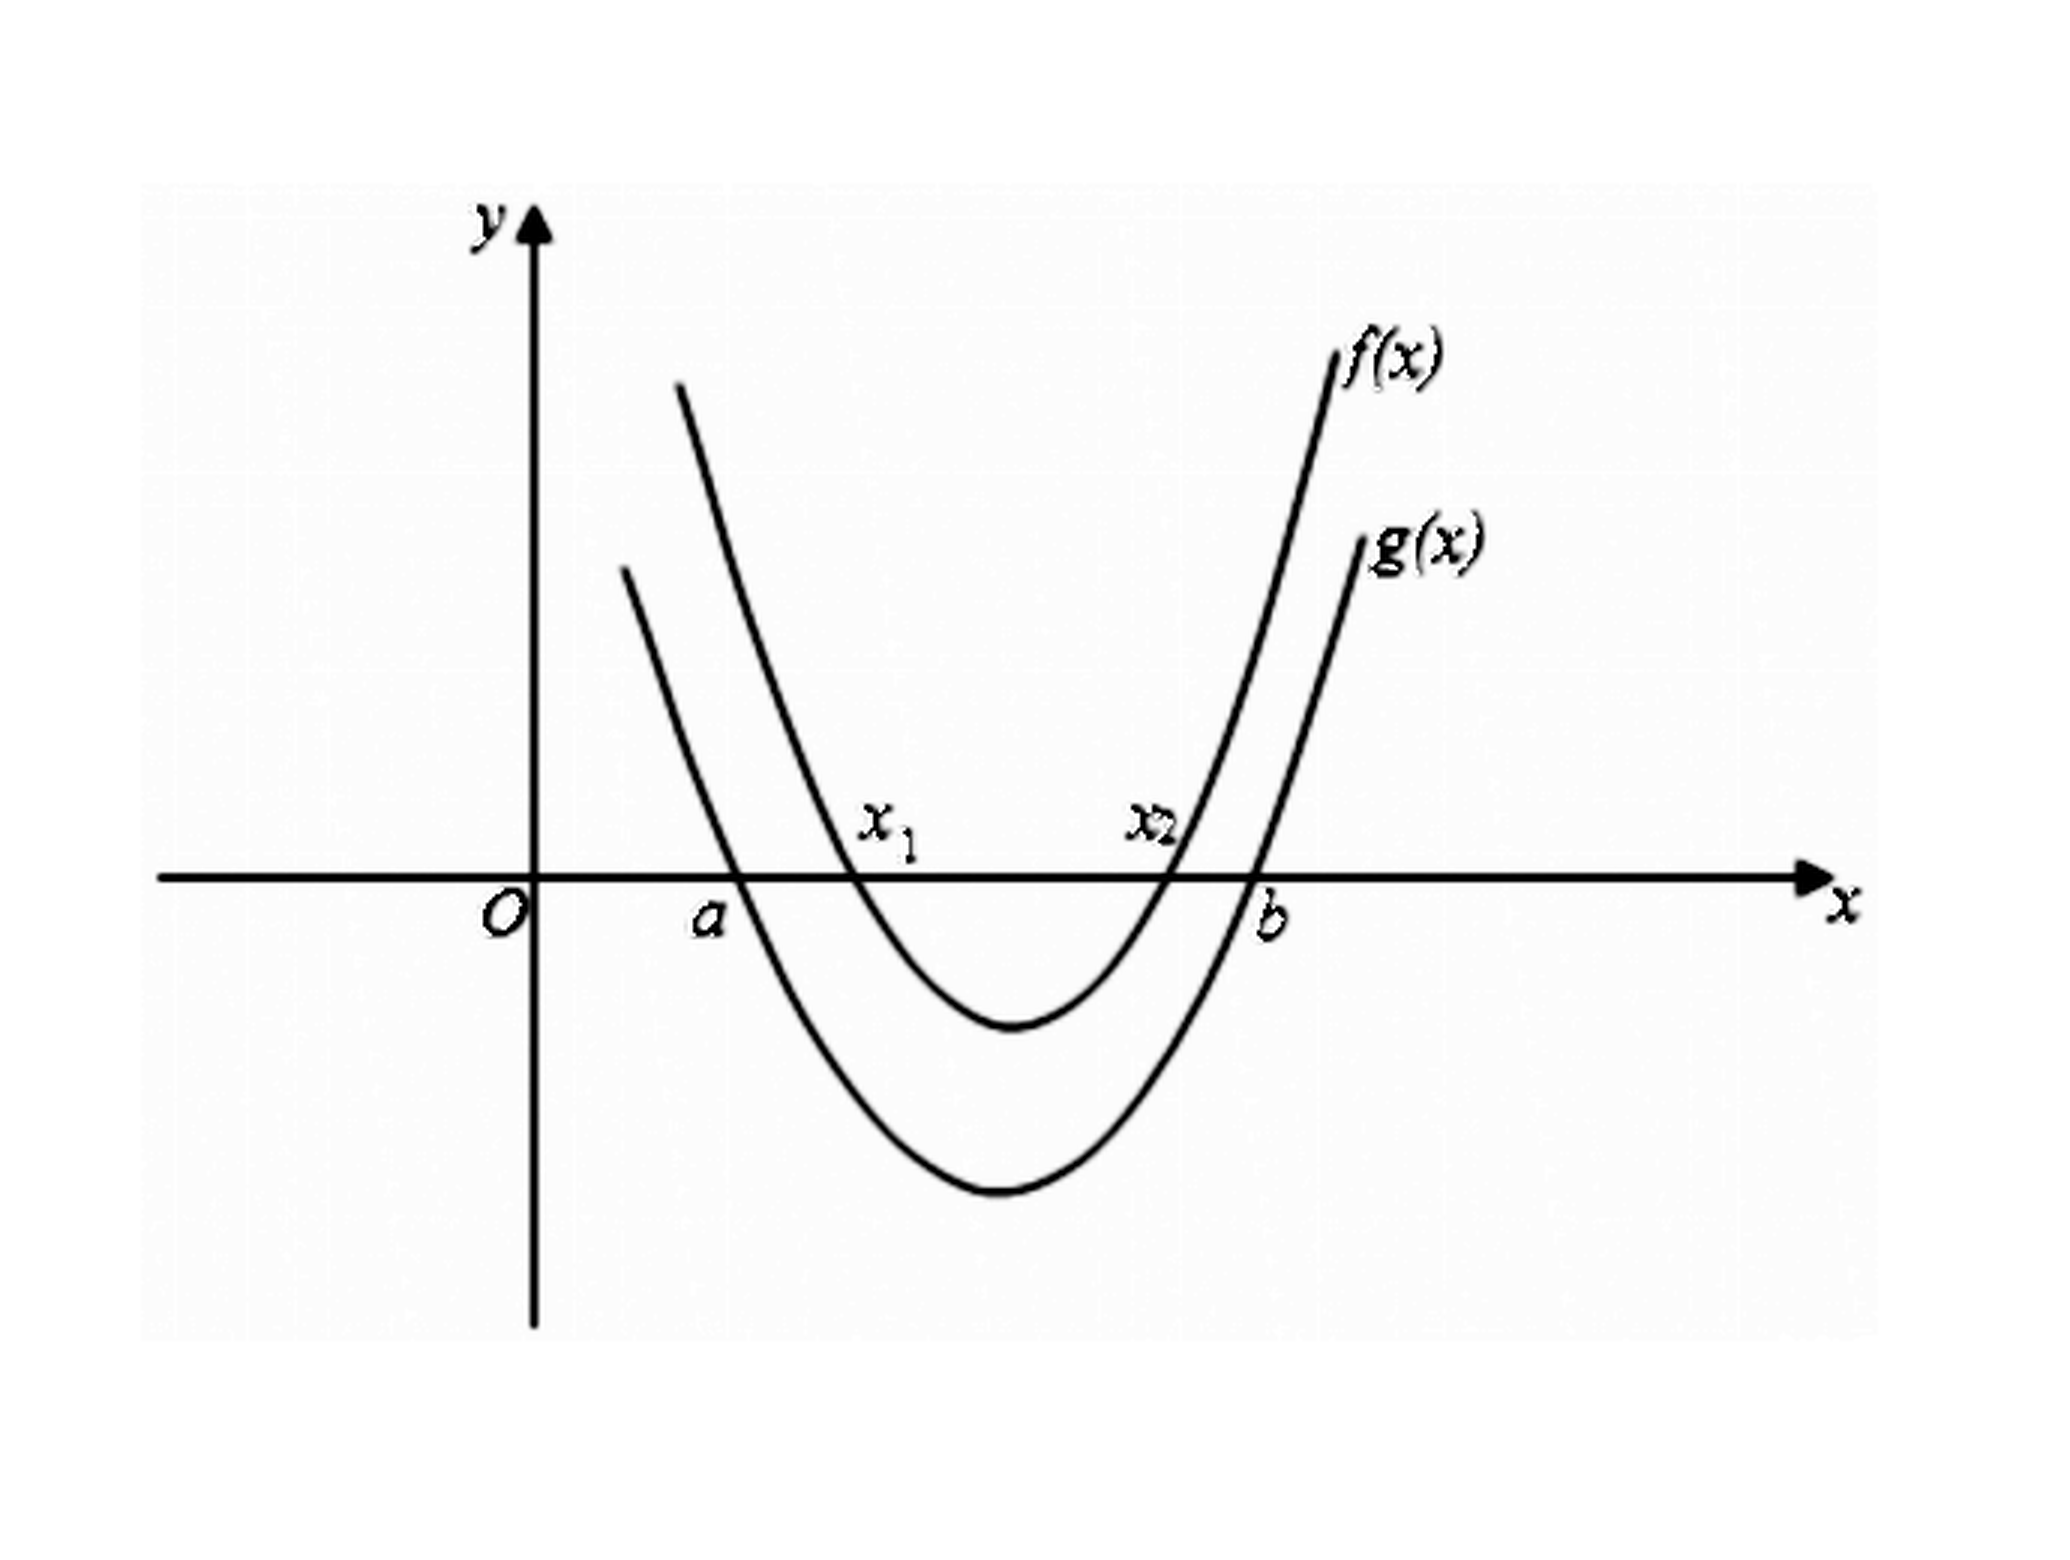
\includegraphics[width=0.52\textwidth]{figures/gao157_q16.png}
\end{center}

\step{由图像得 $a<x_1<x_2<b$，故选 $A$.}
\solend
\fi

\end{enumerate}

\bigsec{三、解答题}

\begin{enumerate}
\setcounter{enumi}{16}

% === Q17 === 解析 6 行；\overline{A}、\varnothing、\subseteq 无、cases
\item 设全集为 $\R$，$m\in\R$，集合 $A=\{x\mid 2<x<5\}$，$B=\{x\mid 2m\leqslant x\leqslant 5m-3\}$.

(1) 若 $m=2$，求 $\overline{A}\cup B$；

(2) 若 $A\cap B=B$，求 $m$ 的取值范围.

\ifanswer
\solbegin
\step{(1) $\overline{A}=\{x\mid x\leqslant2$ 或 $x\geqslant5\}$，当 $m=2$ 时，$B=\{x\mid 4\leqslant x\leqslant7\}$，}
\step{则 $\overline{A}\cup B=\{x\mid x\leqslant2$ 或 $x\geqslant4\}$；}
\step{(2) 因为 $A\cap B=B$，所以 $B$ 是 $A$ 的子集，}
\step{当 $B=\varnothing$ 时，$2m>5m-3$，解得 $m<1$；}
\step{当 $B\ne\varnothing$ 时，$\begin{cases}2m\leqslant5m-3\\2m>2\\5m-3<5\end{cases}$，解得 $1<m<\dfrac85$；}
\step{综上，$m$ 的取值范围是 $(-\infty,1)\cup\left(1,\dfrac85\right)$.}
\solend
\fi

% === Q18 === 解析 2 行；指数式、\lg、换底
\item (1) 设 $a^{2x}=3$，且 $a>0$，求 $\dfrac{a^{3x}+a^{-3x}}{a^x+a^{-x}}$ 的值；

(2) 已知 $\lg2=a, 10^b=3$，用 $a$ 及 $b$ 表示 $\log_{12}25$.

\ifanswer
\solbegin
\step{(1) $\dfrac{a^{3x}+a^{-3x}}{a^x+a^{-x}}=a^{2x}-1+a^{-2x}=3-1+\dfrac13=\dfrac73$；}
\step{(2) $\log_{12}25=\dfrac{\lg25}{\lg12}=\dfrac{2-2\lg2}{2\lg2+\lg3}=\dfrac{2-2a}{2a+b}$.}
\solend
\fi

% === Q19 === 解析 11 行；幂函数、$=0$ 笔误照录、\Delta、\sqrt5、cases
\item 已知幂函数 $f(x)=(m^2+m-1)x^{-2m^2+m+3}$ 在 $(0,+\infty)$ 上为严格增函数.

(1) 求 $f(x)$ 的解析式；

(2) 若 $k+kf(x)>f(x)-x-1$ 对任意实数 $x$ 都成立，求实数 $k$ 的取值范围；

(3) 若关于 $x$ 的不等式 $f(x)\leqslant8x-a$ 的解集中有且仅有 $5$ 个整数，求实数 $a$ 的范围.

\ifanswer
\solbegin
\step{(1) 由题意得 $m^2+m-1=1$，且 $-2m^2+m+3>0$，}
\step{解得 $m=-2$（舍去）或 $m=1$，所以 $f(x)=x^2$；}
\step{(2) $k+kf(x)>f(x)-x-1$ 可化为 $(k-1)x^2+x+k+1=0$ 恒成立，}
\step{当 $k=1$ 时，$x+2>0$，显然不恒成立；}
\step{当 $k\ne1$ 时，要使该二次不等式恒成立，只需 $\begin{cases}k-1>0\\[2pt]\Delta=1-4(k+1)(k-1)\leqslant0\end{cases}$，}
\step{解得 $k\geqslant\dfrac{\sqrt5}{2}$，即所求 $k$ 的范围是 $\left[\dfrac{\sqrt5}{2},+\infty\right)$；}
\step{(3) 不等式 $f(x)\leqslant8x-a$，即 $x^2-8x+a\leqslant0$ 有五个整数解，}
\step{令 $g(x)=x^2-8x+a$，因为该函数开口向上，对称轴为 $x=4$，}
\step{所以解集内的整数为 $2$，$3$，$4$，$5$，$6$，}
\step{由二次函数的性质得，只需 $\begin{cases}g(1)=1-8+a>0\\g(2)=4-8\times2+a\leqslant0\end{cases}$，解得 $7<a\leqslant12$，}
\step{故 $a$ 的取值范围是 $(7,12]$.}
\solend
\fi

% === Q20 === 解析 12 行；材料题、$a+b=1$、大根号、"因出"笔误、分母套分数
\item 问题：正数 $a$、$b$ 满足 $a+b=1$，求 $\dfrac1a+\dfrac2b$ 的最小值.

其中一种解法是：$\dfrac1a+\dfrac2b=\left(\dfrac1a+\dfrac2b\right)(a+b)=1+\dfrac ba+\dfrac{2a}{b}+2\geqslant3+2\sqrt2$，

当且仅当 $\dfrac ba=\dfrac{2a}{b}$ 且 $a+b=1$ 时，即 $a=\sqrt2-1$ 且 $b=2-\sqrt2$ 时取等号.

学习上述解法并解决下列问题：

(1) 若正实数 $x$、$y$ 满足 $x+y=1$，求 $\dfrac2x+\dfrac1y$ 的最小值；

(2) 若实数 $a$、$b$、$x$、$y$ 满足 $\dfrac{x^2}{a^2}-\dfrac{y^2}{b^2}=1$，求证：$a^2-b^2\leqslant(x-y)^2$；

(3) 利用 (2) 的结论，求代数式 $M=\sqrt{2m-5}-\sqrt{m-3}$ 的最小值，并求出使得 $M$ 最小的 $m$ 的值.

\ifanswer
\solbegin
\step{(1) $\dfrac2x+\dfrac1y=(x+y)\left(\dfrac2x+\dfrac1y\right)=3+\dfrac xy+\dfrac{2y}{x}\geqslant3+2\sqrt2$，}
\step{当且仅当 $\dfrac xy=\dfrac{2y}{x}$ 且 $x+y=1$ 时取等号；}
\step{(2) $a^2-b^2=(a^2-b^2)\left(\dfrac{x^2}{a^2}-\dfrac{y^2}{b^2}\right)=x^2+y^2-\left(\dfrac{a^2x^2}{b^2}+\dfrac{b^2y^2}{a^2}\right)$}
\step{$\leqslant x^2+y^2-2\sqrt{\dfrac{a^2x^2}{b^2}\cdot\dfrac{b^2y^2}{a^2}}=x^2+y^2-2xy=(x-y)^2$，}
\step{故当 $b^4x^2=a^4y^2$ 时，等号成立.}
\step{(3) 令 $x=\sqrt{2m-5}, y=\sqrt{m-3}$，由 $\begin{cases}2m-5\geqslant0\\m-3\geqslant0\end{cases}$ 得 $m\geqslant3$，}
\step{$x^2-y^2=(2m-5)-(m-3)=m-2>0$，}
\step{又 $x>0, y>0$，所以 $x>y$，所以 $\dfrac{x^2}{a^2}-\dfrac{y^2}{b^2}=1$，}
\step{由 $x^2-2y^2=1$，得 $\dfrac{x^2}{1}-\dfrac{y^2}{\frac12}=1$，因出 $a^2=1, b^2=\dfrac12$，}
\step{由 (2) 得 $M=\sqrt{2m-5}-\sqrt{m-3}=x-y\geqslant\sqrt{a^2-b^2}=\sqrt{1-\dfrac12}=\dfrac{\sqrt2}{2}$，}
\step{当且仅当 $\dfrac xy=\left(\dfrac ab\right)^2=2$ 取等号，结合 $x^2-2y^2=1$，解得 $x=\sqrt2, y=\dfrac{\sqrt2}{2}$，}
\step{即 $\sqrt{2m-5}=\sqrt2$，得 $m=\dfrac72$，所以 $m=\dfrac72$ 时，$M$ 取得最小值 $\dfrac{\sqrt2}{2}$.}
\solend
\fi

\end{enumerate}

\end{document}
"
%
% ① 原始材料：微信公众号"魔都数学加油站"文章，连载"27学年高一157"，原文标题
% "27学年高一157——2026-2027年上海市大境中学高一上期中"；
% 原文链接：https://mp.weixin.qq.com/s/s6eDMDVkxc2fcBe8LNm-Tw 。
% 正文为 8 张 PNG 页（01/02/03/04/06 为 4762×6735，05/07/08 为 2560×3620，
% 同一篇各页分辨率混排，逐页按各自分辨率裁图核对）。
% 体例：讲评版——填空 3—12（10 题）、选择 13—16（4 题）、解答 17—20（4 题），
% 共 18 题，自第 3 题起编（1、2 未印在本篇）；末题是第 20 题（不是 21）。
% 除第 4 题只印【答案】外，其余 17 题逐题印【解析】（逐题核实，见 ②）。
% 题目、答案、解析均据原图转录；卷面粉红色水印"魔都数学加油站"及公众号
% 页脚未录入。
% 全卷仅 1 幅配图：第 16 题解析内函数图像（"设 g(x)=(x-a)(x-b)，
% f(x)=g(x)+1，画出函数 g(x) 与函数 f(x) 的图像，如图所示"），
% 解析内配图仅答案版出，裁 figures/gao157_q16.png；逐页通读 8 页确认
% 无题目配图、无表格；08 页下半仅水印、无正文。
%
% 卷首标题：原卷印作"2026-2027 年大境中学高一上期中"，年份区间按全稿惯例排 en dash；
% 原卷卷面未印副标题，本稿按同期中卷知识模块口径补出"集合与常用逻辑用语、不等式、函数"。
%
% ② 与原卷的排版差异：
%   ① 原文从第 3 题起，本稿保留原题号；共 18 题三节，解答题 4 题到 20；
%      三节各自 \begin{enumerate}…\end{enumerate} + \setcounter{enumi}{2/12/16}
%      （题目溯源.py 按 \bigsec 切节、每节独立计 depth，只收 depth==1 的 \item，
%       见 高一156 头注②的订正）；
%   ② 第 4 题只印【答案】、无【解析】，提 \ans{}；其余 17 题逐题印【解析】、
%      逐题设 \solbegin…\solend；四道选择题答案在解析末句"故选 D／D／C／A"
%      （逐个放大复核）、括号 \mbox{（\quad）} 留空；答案版【答案】/【解析】
%      标记数 = 18 = 全卷题数（1 个 \ans ＋ 17 个 \solbegin）；
%   ③ 原卷卷面未印副标题，本稿按知识模块口径补出；
%   ④ 原卷填空横线按全稿惯例排 \blankline[4.4em]；选择题选项段前按惯例各加
%      \keepwithprev；解答题不留作答区、不加 \anspace（原卷为讲评版，109—113 起
%      全稿不用 \anspace）；
%   ⑤ 数集：Q4"$x、y\in R$"、Q6"$x\in R$"、Q10"$a\in Z$"、Q12"$n\in Z$"
%      "$n_1、n_2\in Z$"、Q17"全集为 R／$m\in R$"原卷印斜体 R/Z，按全稿惯例
%      归一 \R／\Z（参见 高一14 头注④、高一150 头注②⑤、高一153 头注⑤）；
%      绝对值排 \lvert…\rvert（Q6 $\lvert x-1\rvert$／$\lvert x+3\rvert$／
%      $\lvert 2x+2\rvert$），集合描述竖线排 \mid（Q12、Q17），空集 \varnothing
%      （Q17"$B=\varnothing$"），补集照原卷上划线排 \overline{A}（Q17），
%      不等号按全稿惯例排 \leqslant／\geqslant；
%   ⑥ 判别式三处（Q8"$\Delta=(-2m)^2-4(m+2)$"、Q15"$\Delta=(a+2)^2+4(a^2-4)<0$"、
%      Q19"$\Delta=1-4(k+1)(k-1)\leqslant0$"）放大比对同形、均为等腰偏高且右斜边
%      加粗的 \Delta，统一照录 \Delta；本卷无扁三角 \triangle 用例（与 高一142／
%      高一151／高一152 的 Δ/△ 混用卷不同）；
%   ⑦ "图像／图象"逐处照录不统一：Q9"图像过点 $(4,2)$""它的图像过点"、
%      Q16"画出函数 $g(x)$ 与函数 $f(x)$ 的图像""由图像得"用"图像"；
%      Q14 题干及解析四处均用"图象"（"的图象关于原点对称""图象关于 $y$ 轴对称"）；
%   ⑧ 原卷笔误／未化简式照录：
%      · Q5 解析"$2\sqrt4+1=5$"根号 4 原卷未化简，照录 \sqrt4；
%      · Q7 解析"$\lg\frac{E_1}{E_2}=\frac25\cdot(m_2-m_1)=\frac25(-1.45+26.7)=10.1$"
%        第一处有 \cdot、第二处无，逐处照录；题干"$m_1-m_2=-\frac52\lg\frac{E_1}{E_2}$"；
%      · Q10 解析"$f(1)=\frac{a+1}{1+2}\geqslant0$"与 cases 第二行分母均印 $1+2$、
%        未化简成 $3$，照录；
%      · Q19 (2)"可化为 $(k-1)x^2+x+k+1=0$ 恒成立"原卷印 $=0$（与 >0 恒成立
%        的题意不符），照录笔误；
%      · Q20 (3)"因出 $a^2=1, b^2=\frac12$"原卷印"因出"（当作"因此"），照录；
%      · Q20 (3)"得 $\frac{x^2}{1}-\frac{y^2}{\frac12}=1$"分母套分数、照录；
%   ⑨ 圈数字①②在文本模式（Q15 解析"①当 $a^2-4=0$ 时""②当 $a^2-4\ne0$ 时"，
%      共 2 枚）；子题标号 (1)(2)(3) 半角括号照录；行末西文句点 ASCII `.`；
%      行中全角逗号／顿号照录；半角逗号在数学组之间是全稿惯例、非笔误
%      （Q8"$x_1+x_2=2m, x_1x_2=m+2$"、Q12"$n\in Z$"、Q18"$\lg2=a, 10^b=3$"、
%      Q20"$a^2=1, b^2=\frac12$"等）；中文弯引号""照录（Q4 命题）；
%   ⑩ 自定义名词：Q11"交叉数"、Q12"$a\otimes b$"新定义运算、Q20"问题／
%      其中一种解法是／学习上述解法并解决下列问题"材料题，均照原卷录入；
%   ⑪ 配图：全卷 1 幅（逐页通读 8 页确认）——Q16 解析内函数图像（05 页右侧，
%      $f(x)$ 与 $g(x)$ 两条抛物线、标注 $a,x_1,x_2,b$），仅答案版出，
%      裁 figures/gao157_q16.png，去粉色水印、去色、3× LANCZOS 放大；
%      图放 \ifanswer 内 \solbegin…\solend 的两 \step 之间（高一108 第 6 题／
%      高一156 Q15 成例）；Q16 题干无"如图"、不需题目配图守卫。
%
% ③ 行数复核：一条 \step = 原卷解析的一个印刷行，cases 块作一个印刷行计；
%    跨半页重叠行（Q5 的"【解析】x-1>0…"、Q10 的"所以 a=-1 或 a=0"、
%    Q12 的"【解析】由 u⊗v…"、Q14 的"f(x)=x² 图象关于 y 轴对称"、
%    Q19 的"(1) 由题意得…"、Q20 的"(3) 令 x=…"等 hi_1/hi_2 两半页共有的行）
%    只计一次，别把原卷折行并起来。
%    逐题数（主会话逐页核对定稿）：Q3：1；Q4：0（只印【答案】、提 \ans{}，
%    不计入 \step 账）；Q5：2；Q6：5；Q7：2；Q8：5；Q9：3；Q10：4；
%    Q11：3；Q12：6；Q13：3；Q14：5；Q15：9；Q16：4；Q17：6；Q18：2；
%    Q19：11；Q20：12。合计 83 条 \step（本卷无 \stepm），与原卷逐题印刷行相等。
%    全卷 18 题：1 题只印【答案】（\ans）、17 题印【解析】（\solbegin…\solend），
%    答案版【答案】/【解析】标记数 = 18 = 全卷题数。
%    全卷除此 6 类外未发现其它笔误／自相矛盾处；17 题印【解析】、1 题印【答案】。
%
\documentclass[a4paper,11pt]{article}
\usepackage{common}

\begin{document}

\examtitlest[3]{2026--2027 年大境中学高一上期中}{集合与常用逻辑用语、不等式、函数}

\bigsec{一、填空题}

\begin{enumerate}
\setcounter{enumi}{2}

% === Q3 === 解析 1 行；$a,b$ 半角逗号照录
\item 若 $a=x^2-2x+1$，$b=x-3$，则 $a,b$ 的大小关系为\blankline[4.4em].

\ifanswer
\solbegin
\step{$a-b=x^2-3x+4=\left(x-\dfrac32\right)^2+\dfrac74>0$，所以 $a>b$.}
\solend
\fi

% === Q4 === 只印【答案】、无【解析】；中文弯引号、\R、顿号；提 \ans{}
\item 用反证法证明命题：“设 $x$、$y\in\R$. 若 $x+y>2$，则 $x>1$ 或 $y>1$”时，假设的内容应该是\blankline[4.4em].

\ifanswer
\ans{$x\leqslant1$ 且 $y\leqslant1$}
\fi

% === Q5 === 解析 2 行；$2\sqrt4+1=5$ 根号 4 未化简照录
\item 当 $x>1$ 时，$x+\dfrac4{x-1}$ 的最小值为\blankline[4.4em].

\ifanswer
\solbegin
\step{$x-1>0$，$x+\dfrac4{x-1}=(x-1)+\dfrac4{x-1}+1\geqslant2\sqrt4+1=5$，}
\step{当且仅当 $x-1=\dfrac4{x-1}$，即 $x=3$ 时取等号，故最小值为 $5$.}
\solend
\fi

% === Q6 === 解析 5 行；绝对值 \lvert…\rvert、\cup、\R
\item 设 $x\in\R$，方程 $\lvert x-1\rvert+\lvert x+3\rvert=\lvert 2x+2\rvert$ 的解集是\blankline[4.4em].

\ifanswer
\solbegin
\step{当 $x\leqslant-3$ 时，方程为 $1-x-x-3=-2x-2$，等式成立；}
\step{当 $-3<x\leqslant-1$ 时，方程为 $1-x+x+3=-2x-2$，解得 $x=-3$，舍去；}
\step{当 $-1<x<1$ 时，方程为 $1-x+x+3=2x+2$，解得 $x=1$，舍去；}
\step{当 $x\geqslant1$ 时，方程为 $x-1+x+3=2x+2$，等式成立，}
\step{综上，方程 $\lvert x-1\rvert+\lvert x+3\rvert=\lvert 2x+2\rvert$ 的解集为 $(-\infty,-3]\cup[1,+\infty)$.}
\solend
\fi

% === Q7 === 解析 2 行；星等材料题、\lg、\cdot 逐处照录、天狼星
\item 在天文学中，天体的明暗程度可以用星等或亮度来描述，两颗星的星等与亮度满足 $m_1-m_2=-\dfrac52\lg\dfrac{E_1}{E_2}$，其中星等为 $m_k$ 的星的亮度为 $E_k(k=1,2)$. 已知太阳的星等为 $-26.7$，天狼星的星等为 $-1.45$，则太阳与天狼星的亮度的比值为\blankline[4.4em].

\ifanswer
\solbegin
\step{两颗星的星等与亮度满足 $m_1-m_2=-\dfrac52\lg\dfrac{E_1}{E_2}$，令 $m_2=-1.45$，$m_1=-26.7$，}
\step{$\lg\dfrac{E_1}{E_2}=\dfrac25\cdot(m_2-m_1)=\dfrac25(-1.45+26.7)=10.1$，$\dfrac{E_1}{E_2}=10^{10.1}$.}
\solend
\fi

% === Q8 === 解析 5 行；韦达定理、判别式 \Delta、半角逗号在数学组间
\item 已知方程 $x^2-2mx+m+2=0$ 有两个实数根 $x_1,x_2$，满足 $x_1^2+x_2^2=2$，则实数 $m$ 的值为\blankline[4.4em].

\ifanswer
\solbegin
\step{对于方程 $x^2-2mx+m+2=0$，由韦达定理得 $x_1+x_2=2m, x_1x_2=m+2$，}
\step{又 $x_1^2+x_2^2=(x_1+x_2)^2-2x_1x_2=(2m)^2-2(m+2)=4m^2-2m-4=2$，}
\step{解得 $m=\dfrac32$ 或 $m=-1$，}
\step{因为方程有两个实数根，所以 $\Delta=(-2m)^2-4(m+2)=4m^2-4m-8\geqslant0$，}
\step{解得 $m\leqslant-1$ 或 $m\geqslant2$，故 $m=-1$.}
\solend
\fi

% === Q9 === 解析 3 行；"图像"照录、$x^\alpha$、$x^{1/2}=\sqrt{x}$
\item 已知幂函数 $y=f(x)$ 的图像过点 $(4,2)$，则不等式 $f(x^2-2x)<f(2-x)$ 的解集为\blankline[4.4em].

\ifanswer
\solbegin
\step{设幂函数 $y=f(x)=x^\alpha$，它的图像过点 $(4,2)$，所以 $4^\alpha=2$，$\alpha=\dfrac12$，}
\step{故 $f(x)=x^{\frac12}=\sqrt{x}$，由不等式 $f(x^2-2x)<f(2-x)$，}
\step{得 $0\leqslant x^2-2x<2-x$，得 $-1<x\leqslant0$，故解集为 $(-1,0]$.}
\solend
\fi

% === Q10 === 解析 4 行；$a\in\Z$、cases（分母 $1+2$ 未化简）、参数分离
\item 已知函数 $y=\dfrac{ax+1}{x+2}$（常数 $a\in\Z$）. 要使该函数在区间 $[1,+\infty)$ 上是严格减函数，并且函数值不恒为负，则满足条件的 $a$ 的取值为\blankline[4.4em].

\ifanswer
\solbegin
\step{函数参数分离为 $y=\dfrac{a(x+2)+1-2a}{x+2}=a+\dfrac{1-2a}{x+2}$，}
\step{若函数在区间 $[1,+\infty)$ 上严格减函数，则 $1-2a>0$，}
\step{且函数的最大值 $f(1)=\dfrac{a+1}{1+2}\geqslant0$，即 $\begin{cases}1-2a>0\\[2pt]\dfrac{a+1}{1+2}\geqslant0\end{cases}$，解得 $-1\leqslant a<\dfrac12$，又 $a\in\Z$，}
\step{所以 $a=-1$ 或 $a=0$.}
\solend
\fi

% === Q11 === 解析 3 行；"交叉数"自定义名词、$(-1)^t$、$2^5$、$32\times3=96$
\item 对非空集合 $A$ 中的每个元素 $t$，都乘以 $(-1)^t$ 再求和，称为集合 $A$ 的交叉数，例如 $A=\{2,3,6\}$，则集合 $A$ 的交叉数为 $(-1)^2\cdot2+(-1)^3\cdot3+(-1)^6\cdot6=5$. 若集合 $W=\{1,2,3,4,5,6\}$，则 $W$ 的所有非空子集的交叉数的总和为\blankline[4.4em].

\ifanswer
\solbegin
\step{固定 $W$ 中的任一元素，其余 $5$ 个元素各有选或不选两种情况，}
\step{因此该元素出现在 $2^5$ 个非空子集中，}
\step{所有交叉数的总和为 $2^5(-1+2-3+4-5+6)=32\times3=96$.}
\solend
\fi

% === Q12 === 解析 6 行；\otimes、\lambda、\mid、\Z、\times 与 \cdot 逐处照录
\item 对于任意两个正实数 $a$、$b$，定义 $a\otimes b=\lambda\cdot\dfrac ab$，其中常数 $\lambda\in\left(\dfrac{\sqrt2}{2},1\right)$. 若 $u\geqslant v>0$，且 $u\otimes v$ 与 $v\otimes u$ 都是集合 $\left\{x\mid x=\dfrac n2,n\in\Z\right\}$ 的元素，则 $u\otimes v=$\blankline[4.4em].

\ifanswer
\solbegin
\step{由 $u\otimes v$ 与 $v\otimes u$ 都是集合 $\left\{x\mid x=\dfrac n2,n\in\Z\right\}$ 的元素，}
\step{不妨设 $\lambda\times\dfrac uv=\dfrac12 n_1$，$\lambda\times\dfrac vu=\dfrac12 n_2$，$n_1$、$n_2\in\Z$，}
\step{因为 $u\geqslant v>0$，所以 $0<\dfrac vu\leqslant1$，因为 $\lambda\in\left(\dfrac{\sqrt2}{2},1\right)$，所以 $\dfrac12 n_2=\lambda\cdot\dfrac vu\in(0,1)$，}
\step{因为 $n_2\in\Z$，所以 $n_2=1$，即 $\dfrac12=\dfrac{\lambda v}{u}$，所以 $\lambda=\dfrac{u}{2v}\in\left(\dfrac{\sqrt2}{2},1\right)$，}
\step{所以 $\dfrac uv\in(\sqrt2,2)$，$\dfrac{u^2}{v^2}\in(2,4)$，则 $\lambda\cdot\dfrac uv=\dfrac{u^2}{v^2}\times\dfrac12=\dfrac12 n_1\in(1,2)$，}
\step{因为 $n_1\in\Z$，所以 $n_1=3$，$\dfrac12 n_1=\dfrac32$，故 $u\otimes v=\dfrac32$.}
\solend
\fi

\end{enumerate}

\bigsec{二、选择题}

\begin{enumerate}
\setcounter{enumi}{12}

% === Q13 === 解析 3 行；选项段 \keepwithprev；故选 D
\item 下列不等式成立的为\mbox{（\quad）}

\keepwithprev
A. 若 $a>b$，则 $ac^2>bc^2$\qquad B. 若 $a>b$，则 $a^2>b^2$

C. 若 $a>b$，$c>d$，则 $a+b>c+d$\qquad D. 若 $a>b$，则 $a^3>b^3$

\ifanswer
\solbegin
\step{A 中 $c=0$ 时不成立；B 取 $a=1$，$b=-2$ 不成立；}
\step{C 取 $a=1$，$b=0$，$c=5$，$d=0$ 不成立.}
\step{幂函数 $y=x^3$ 在实数集上严格递增，所以 $a>b\Rightarrow a^3>b^3$，故选 $D$.}
\solend
\fi

% === Q14 === 解析 5 行；"图象"四处照录；故选 D
\item 幂函数 $f(x)=x^\alpha$ 的图象关于原点对称，且在 $(-\infty,0)$ 上是严格增函数，则 $f(x)$ 可以是\mbox{（\quad）}

\keepwithprev
A. $f(x)=x^{-1}$\qquad B. $f(x)=x^{\frac12}$\qquad C. $f(x)=x^2$\qquad D. $f(x)=x^3$

\ifanswer
\solbegin
\step{$f(x)=\dfrac1x$ 的图象关于原点对称，在 $(-\infty,0)$ 上是严格减函数，故 $A$ 错误；}
\step{$f(x)=x^{\frac12}$ 在 $(-\infty,0)$ 上无意义，故 $B$ 错误；}
\step{$f(x)=x^2$ 图象关于 $y$ 轴对称，故 $C$ 错误；}
\step{$f(x)=x^3$ 的图象关于原点对称，且在 $(-\infty,0)$ 上是严格增函数，故 $D$ 正确.}
\step{故选 $D$.}
\solend
\fi

% === Q15 === 解析 9 行；圈数字①②、\Delta、cases；故选 C
\item 若关于 $x$ 的不等式 $(a^2-4)x^2+(a+2)x-1\geqslant0$ 的解集不为空集，则实数 $a$ 的取值范围为\mbox{（\quad）}

\keepwithprev
A. $\left(-2,\dfrac65\right]$\qquad B. $\left[-2,\dfrac65\right]$

C. $(-\infty,-2)\cup\left[\dfrac65,+\infty\right)$\qquad D. $(-\infty,-2]\cup\left[\dfrac65,+\infty\right)$

\ifanswer
\solbegin
\step{①当 $a^2-4=0$ 时，$a=\pm2$，}
\step{若 $a=2$ 时，原不等式为 $4x-1\geqslant0$，则不等式的解集不是空集；}
\step{若 $a=-2$ 时，原不等式为 $-1\geqslant0$，无解，不符合题意；}
\step{②当 $a^2-4\ne0$ 时，$a\ne\pm2$，}
\step{若 $(a^2-4)x^2+(a+2)x-1\geqslant0$ 的解集是空集，则 $\begin{cases}a^2-4<0\\[2pt]\Delta=(a+2)^2+4(a^2-4)<0\end{cases}$，}
\step{解得 $-2<a<\dfrac65$，}
\step{则当不等式 $(a^2-4)x^2+(a+2)x-1\geqslant0$ 的解集不为空集时，}
\step{有 $a<-2$ 或 $a\geqslant\dfrac65$ 且 $a\ne2$，}
\step{综上，实数 $a$ 的取值范围为 $(-\infty,-2)\cup\left[\dfrac65,+\infty\right)$，故选 $C$.}
\solend
\fi

% === Q16 === 解析 4 行＋1 幅解析内配图（仅答案版）；"图像"照录；故选 A
\item 已知实数 $a<b$，关于 $x$ 的不等式 $x^2-(a+b)x+ab+1<0$ 的解集为 $(x_1,x_2)$，则实数 $a$、$b$、$x_1$、$x_2$ 从小到大的排列是\mbox{（\quad）}

\keepwithprev
A. $a<x_1<x_2<b$\qquad B. $x_1<a<b<x_2$\qquad C. $a<x_1<b<x_2$\qquad D. $x_1<a<x_2<b$

\ifanswer
\solbegin
\step{不等式 $x^2-(a+b)x+ab+1<0$ 可化为 $(x-a)(x-b)+1<0$，}
\step{设 $g(x)=(x-a)(x-b)$，$f(x)=g(x)+1$，}
\step{画出函数 $g(x)$ 与函数 $f(x)$ 的图像，如图所示，}

\begin{center}
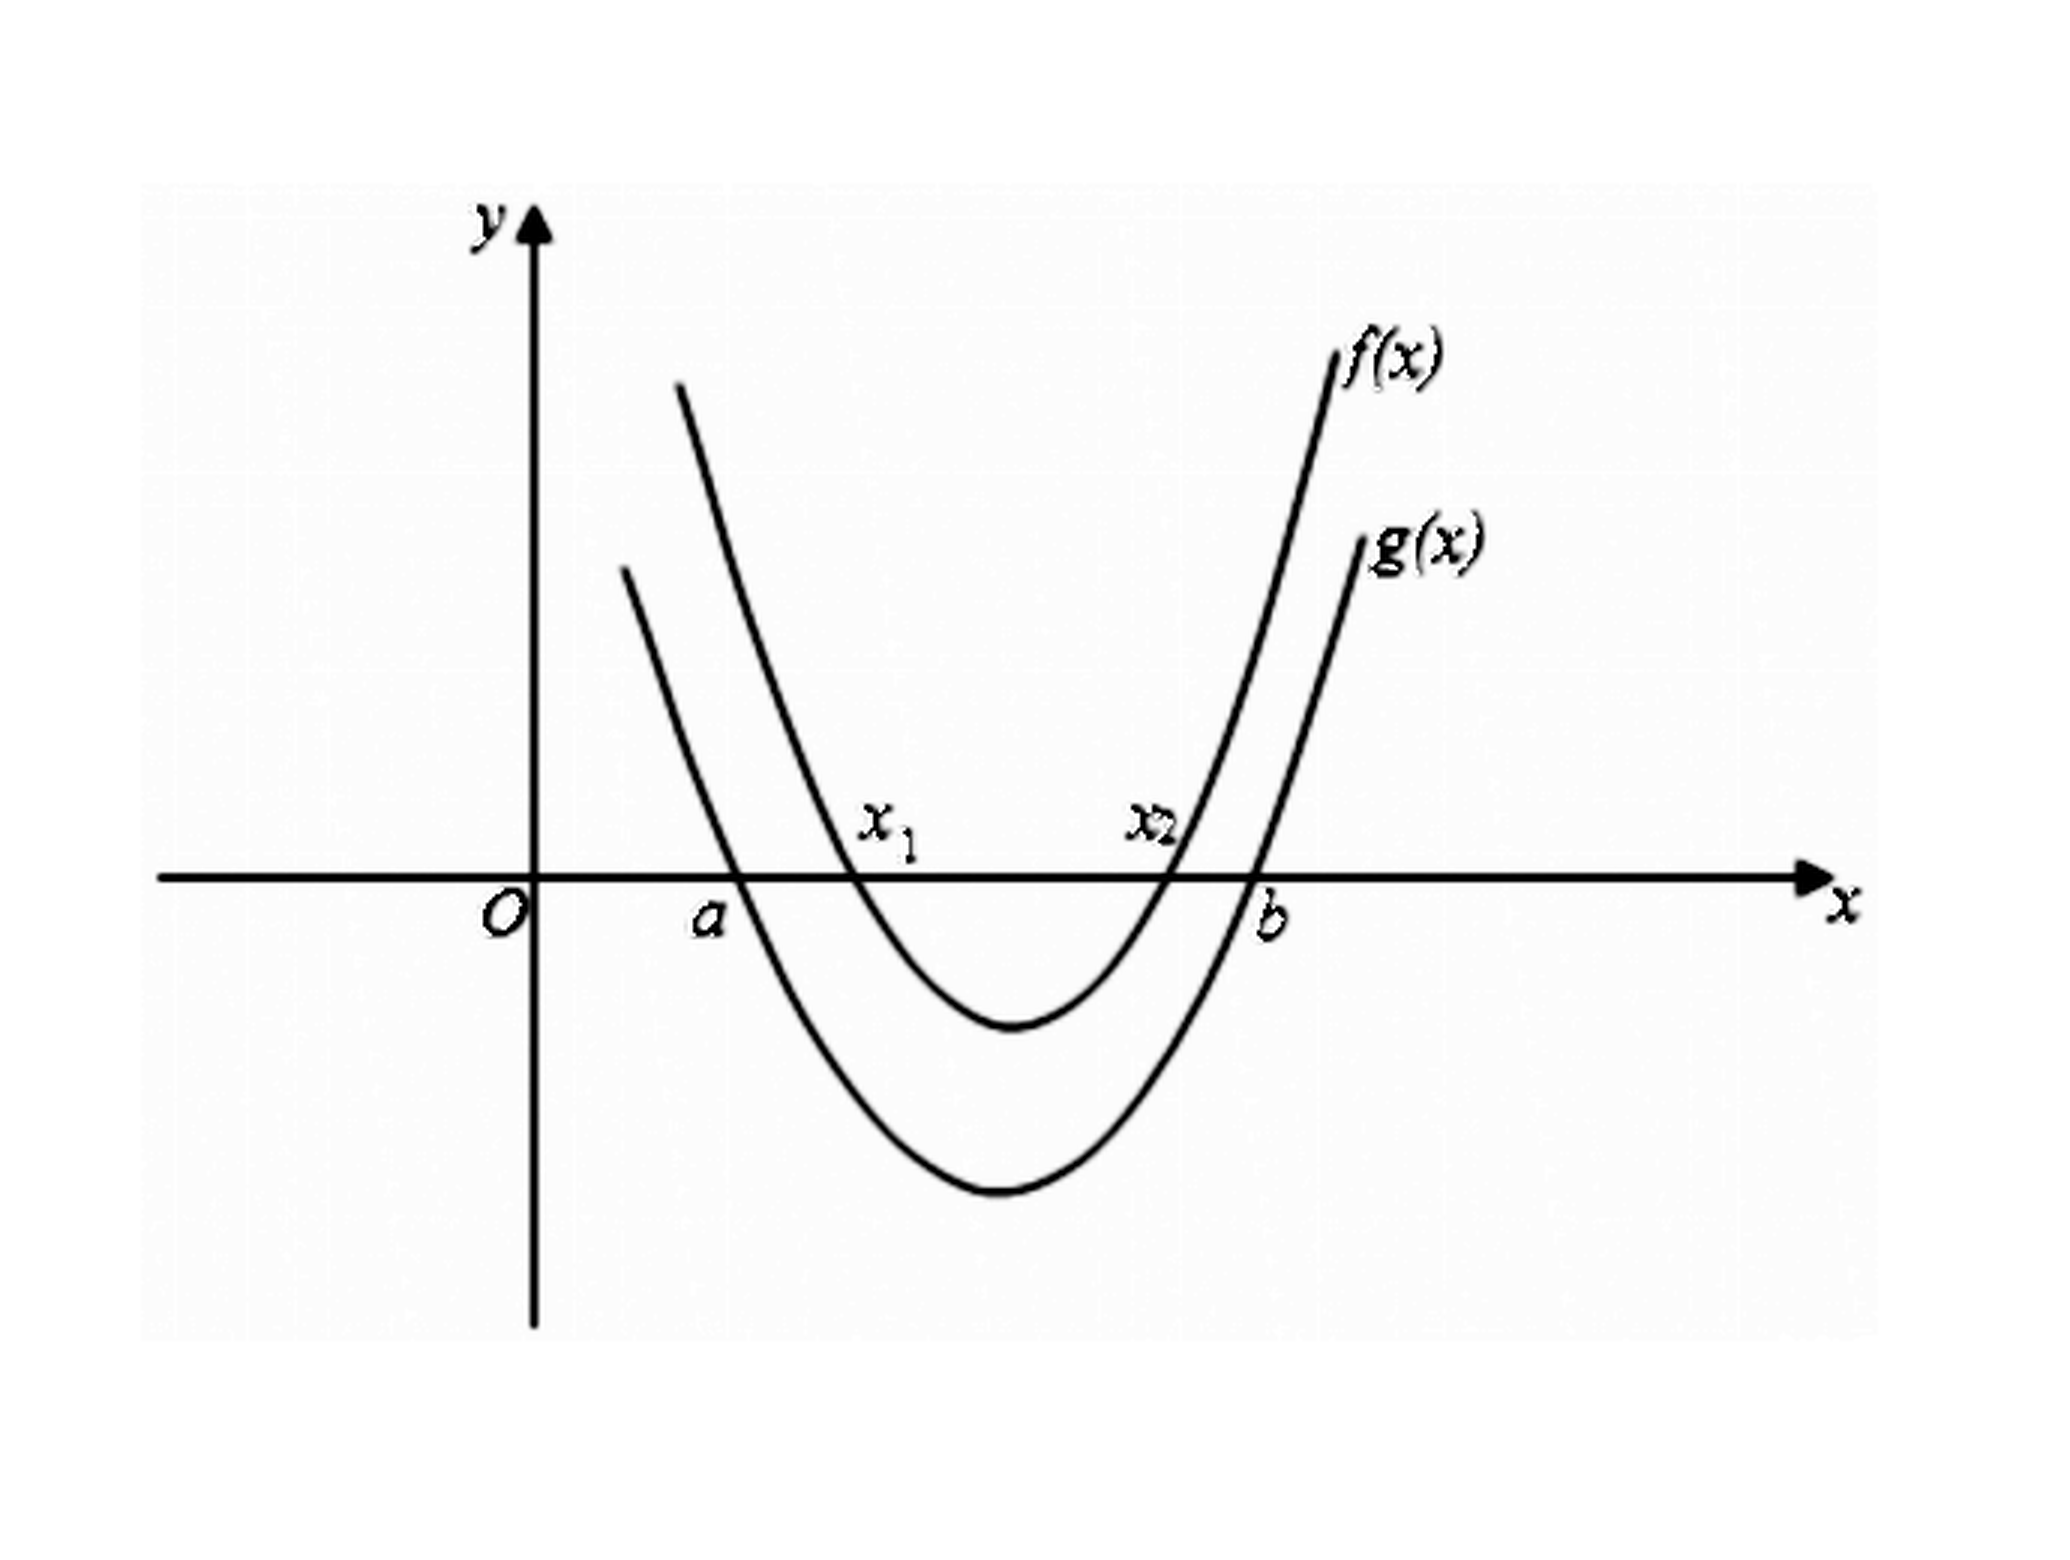
\includegraphics[width=0.52\textwidth]{figures/gao157_q16.png}
\end{center}

\step{由图像得 $a<x_1<x_2<b$，故选 $A$.}
\solend
\fi

\end{enumerate}

\bigsec{三、解答题}

\begin{enumerate}
\setcounter{enumi}{16}

% === Q17 === 解析 6 行；\overline{A}、\varnothing、\subseteq 无、cases
\item 设全集为 $\R$，$m\in\R$，集合 $A=\{x\mid 2<x<5\}$，$B=\{x\mid 2m\leqslant x\leqslant 5m-3\}$.

(1) 若 $m=2$，求 $\overline{A}\cup B$；

(2) 若 $A\cap B=B$，求 $m$ 的取值范围.

\ifanswer
\solbegin
\step{(1) $\overline{A}=\{x\mid x\leqslant2$ 或 $x\geqslant5\}$，当 $m=2$ 时，$B=\{x\mid 4\leqslant x\leqslant7\}$，}
\step{则 $\overline{A}\cup B=\{x\mid x\leqslant2$ 或 $x\geqslant4\}$；}
\step{(2) 因为 $A\cap B=B$，所以 $B$ 是 $A$ 的子集，}
\step{当 $B=\varnothing$ 时，$2m>5m-3$，解得 $m<1$；}
\step{当 $B\ne\varnothing$ 时，$\begin{cases}2m\leqslant5m-3\\2m>2\\5m-3<5\end{cases}$，解得 $1<m<\dfrac85$；}
\step{综上，$m$ 的取值范围是 $(-\infty,1)\cup\left(1,\dfrac85\right)$.}
\solend
\fi

% === Q18 === 解析 2 行；指数式、\lg、换底
\item (1) 设 $a^{2x}=3$，且 $a>0$，求 $\dfrac{a^{3x}+a^{-3x}}{a^x+a^{-x}}$ 的值；

(2) 已知 $\lg2=a, 10^b=3$，用 $a$ 及 $b$ 表示 $\log_{12}25$.

\ifanswer
\solbegin
\step{(1) $\dfrac{a^{3x}+a^{-3x}}{a^x+a^{-x}}=a^{2x}-1+a^{-2x}=3-1+\dfrac13=\dfrac73$；}
\step{(2) $\log_{12}25=\dfrac{\lg25}{\lg12}=\dfrac{2-2\lg2}{2\lg2+\lg3}=\dfrac{2-2a}{2a+b}$.}
\solend
\fi

% === Q19 === 解析 11 行；幂函数、$=0$ 笔误照录、\Delta、\sqrt5、cases
\item 已知幂函数 $f(x)=(m^2+m-1)x^{-2m^2+m+3}$ 在 $(0,+\infty)$ 上为严格增函数.

(1) 求 $f(x)$ 的解析式；

(2) 若 $k+kf(x)>f(x)-x-1$ 对任意实数 $x$ 都成立，求实数 $k$ 的取值范围；

(3) 若关于 $x$ 的不等式 $f(x)\leqslant8x-a$ 的解集中有且仅有 $5$ 个整数，求实数 $a$ 的范围.

\ifanswer
\solbegin
\step{(1) 由题意得 $m^2+m-1=1$，且 $-2m^2+m+3>0$，}
\step{解得 $m=-2$（舍去）或 $m=1$，所以 $f(x)=x^2$；}
\step{(2) $k+kf(x)>f(x)-x-1$ 可化为 $(k-1)x^2+x+k+1=0$ 恒成立，}
\step{当 $k=1$ 时，$x+2>0$，显然不恒成立；}
\step{当 $k\ne1$ 时，要使该二次不等式恒成立，只需 $\begin{cases}k-1>0\\[2pt]\Delta=1-4(k+1)(k-1)\leqslant0\end{cases}$，}
\step{解得 $k\geqslant\dfrac{\sqrt5}{2}$，即所求 $k$ 的范围是 $\left[\dfrac{\sqrt5}{2},+\infty\right)$；}
\step{(3) 不等式 $f(x)\leqslant8x-a$，即 $x^2-8x+a\leqslant0$ 有五个整数解，}
\step{令 $g(x)=x^2-8x+a$，因为该函数开口向上，对称轴为 $x=4$，}
\step{所以解集内的整数为 $2$，$3$，$4$，$5$，$6$，}
\step{由二次函数的性质得，只需 $\begin{cases}g(1)=1-8+a>0\\g(2)=4-8\times2+a\leqslant0\end{cases}$，解得 $7<a\leqslant12$，}
\step{故 $a$ 的取值范围是 $(7,12]$.}
\solend
\fi

% === Q20 === 解析 12 行；材料题、$a+b=1$、大根号、"因出"笔误、分母套分数
\item 问题：正数 $a$、$b$ 满足 $a+b=1$，求 $\dfrac1a+\dfrac2b$ 的最小值.

其中一种解法是：$\dfrac1a+\dfrac2b=\left(\dfrac1a+\dfrac2b\right)(a+b)=1+\dfrac ba+\dfrac{2a}{b}+2\geqslant3+2\sqrt2$，

当且仅当 $\dfrac ba=\dfrac{2a}{b}$ 且 $a+b=1$ 时，即 $a=\sqrt2-1$ 且 $b=2-\sqrt2$ 时取等号.

学习上述解法并解决下列问题：

(1) 若正实数 $x$、$y$ 满足 $x+y=1$，求 $\dfrac2x+\dfrac1y$ 的最小值；

(2) 若实数 $a$、$b$、$x$、$y$ 满足 $\dfrac{x^2}{a^2}-\dfrac{y^2}{b^2}=1$，求证：$a^2-b^2\leqslant(x-y)^2$；

(3) 利用 (2) 的结论，求代数式 $M=\sqrt{2m-5}-\sqrt{m-3}$ 的最小值，并求出使得 $M$ 最小的 $m$ 的值.

\ifanswer
\solbegin
\step{(1) $\dfrac2x+\dfrac1y=(x+y)\left(\dfrac2x+\dfrac1y\right)=3+\dfrac xy+\dfrac{2y}{x}\geqslant3+2\sqrt2$，}
\step{当且仅当 $\dfrac xy=\dfrac{2y}{x}$ 且 $x+y=1$ 时取等号；}
\step{(2) $a^2-b^2=(a^2-b^2)\left(\dfrac{x^2}{a^2}-\dfrac{y^2}{b^2}\right)=x^2+y^2-\left(\dfrac{a^2x^2}{b^2}+\dfrac{b^2y^2}{a^2}\right)$}
\step{$\leqslant x^2+y^2-2\sqrt{\dfrac{a^2x^2}{b^2}\cdot\dfrac{b^2y^2}{a^2}}=x^2+y^2-2xy=(x-y)^2$，}
\step{故当 $b^4x^2=a^4y^2$ 时，等号成立.}
\step{(3) 令 $x=\sqrt{2m-5}, y=\sqrt{m-3}$，由 $\begin{cases}2m-5\geqslant0\\m-3\geqslant0\end{cases}$ 得 $m\geqslant3$，}
\step{$x^2-y^2=(2m-5)-(m-3)=m-2>0$，}
\step{又 $x>0, y>0$，所以 $x>y$，所以 $\dfrac{x^2}{a^2}-\dfrac{y^2}{b^2}=1$，}
\step{由 $x^2-2y^2=1$，得 $\dfrac{x^2}{1}-\dfrac{y^2}{\frac12}=1$，因出 $a^2=1, b^2=\dfrac12$，}
\step{由 (2) 得 $M=\sqrt{2m-5}-\sqrt{m-3}=x-y\geqslant\sqrt{a^2-b^2}=\sqrt{1-\dfrac12}=\dfrac{\sqrt2}{2}$，}
\step{当且仅当 $\dfrac xy=\left(\dfrac ab\right)^2=2$ 取等号，结合 $x^2-2y^2=1$，解得 $x=\sqrt2, y=\dfrac{\sqrt2}{2}$，}
\step{即 $\sqrt{2m-5}=\sqrt2$，得 $m=\dfrac72$，所以 $m=\dfrac72$ 时，$M$ 取得最小值 $\dfrac{\sqrt2}{2}$.}
\solend
\fi

\end{enumerate}

\end{document}
"
%
% ① 原始材料：微信公众号"魔都数学加油站"文章，连载"27学年高一157"，原文标题
% "27学年高一157——2026-2027年上海市大境中学高一上期中"；
% 原文链接：https://mp.weixin.qq.com/s/s6eDMDVkxc2fcBe8LNm-Tw 。
% 正文为 8 张 PNG 页（01/02/03/04/06 为 4762×6735，05/07/08 为 2560×3620，
% 同一篇各页分辨率混排，逐页按各自分辨率裁图核对）。
% 体例：讲评版——填空 3—12（10 题）、选择 13—16（4 题）、解答 17—20（4 题），
% 共 18 题，自第 3 题起编（1、2 未印在本篇）；末题是第 20 题（不是 21）。
% 除第 4 题只印【答案】外，其余 17 题逐题印【解析】（逐题核实，见 ②）。
% 题目、答案、解析均据原图转录；卷面粉红色水印"魔都数学加油站"及公众号
% 页脚未录入。
% 全卷仅 1 幅配图：第 16 题解析内函数图像（"设 g(x)=(x-a)(x-b)，
% f(x)=g(x)+1，画出函数 g(x) 与函数 f(x) 的图像，如图所示"），
% 解析内配图仅答案版出，裁 figures/gao157_q16.png；逐页通读 8 页确认
% 无题目配图、无表格；08 页下半仅水印、无正文。
%
% 卷首标题：原卷印作"2026-2027 年大境中学高一上期中"，年份区间按全稿惯例排 en dash；
% 原卷卷面未印副标题，本稿按同期中卷知识模块口径补出"集合与常用逻辑用语、不等式、函数"。
%
% ② 与原卷的排版差异：
%   ① 原文从第 3 题起，本稿保留原题号；共 18 题三节，解答题 4 题到 20；
%      三节各自 \begin{enumerate}…\end{enumerate} + \setcounter{enumi}{2/12/16}
%      （题目溯源.py 按 \bigsec 切节、每节独立计 depth，只收 depth==1 的 \item，
%       见 高一156 头注②的订正）；
%   ② 第 4 题只印【答案】、无【解析】，提 \ans{}；其余 17 题逐题印【解析】、
%      逐题设 \solbegin…\solend；四道选择题答案在解析末句"故选 D／D／C／A"
%      （逐个放大复核）、括号 \mbox{（\quad）} 留空；答案版【答案】/【解析】
%      标记数 = 18 = 全卷题数（1 个 \ans ＋ 17 个 \solbegin）；
%   ③ 原卷卷面未印副标题，本稿按知识模块口径补出；
%   ④ 原卷填空横线按全稿惯例排 \blankline[4.4em]；选择题选项段前按惯例各加
%      \keepwithprev；解答题不留作答区、不加 \anspace（原卷为讲评版，109—113 起
%      全稿不用 \anspace）；
%   ⑤ 数集：Q4"$x、y\in R$"、Q6"$x\in R$"、Q10"$a\in Z$"、Q12"$n\in Z$"
%      "$n_1、n_2\in Z$"、Q17"全集为 R／$m\in R$"原卷印斜体 R/Z，按全稿惯例
%      归一 \R／\Z（参见 高一14 头注④、高一150 头注②⑤、高一153 头注⑤）；
%      绝对值排 \lvert…\rvert（Q6 $\lvert x-1\rvert$／$\lvert x+3\rvert$／
%      $\lvert 2x+2\rvert$），集合描述竖线排 \mid（Q12、Q17），空集 \varnothing
%      （Q17"$B=\varnothing$"），补集照原卷上划线排 \overline{A}（Q17），
%      不等号按全稿惯例排 \leqslant／\geqslant；
%   ⑥ 判别式三处（Q8"$\Delta=(-2m)^2-4(m+2)$"、Q15"$\Delta=(a+2)^2+4(a^2-4)<0$"、
%      Q19"$\Delta=1-4(k+1)(k-1)\leqslant0$"）放大比对同形、均为等腰偏高且右斜边
%      加粗的 \Delta，统一照录 \Delta；本卷无扁三角 \triangle 用例（与 高一142／
%      高一151／高一152 的 Δ/△ 混用卷不同）；
%   ⑦ "图像／图象"逐处照录不统一：Q9"图像过点 $(4,2)$""它的图像过点"、
%      Q16"画出函数 $g(x)$ 与函数 $f(x)$ 的图像""由图像得"用"图像"；
%      Q14 题干及解析四处均用"图象"（"的图象关于原点对称""图象关于 $y$ 轴对称"）；
%   ⑧ 原卷笔误／未化简式照录：
%      · Q5 解析"$2\sqrt4+1=5$"根号 4 原卷未化简，照录 \sqrt4；
%      · Q7 解析"$\lg\frac{E_1}{E_2}=\frac25\cdot(m_2-m_1)=\frac25(-1.45+26.7)=10.1$"
%        第一处有 \cdot、第二处无，逐处照录；题干"$m_1-m_2=-\frac52\lg\frac{E_1}{E_2}$"；
%      · Q10 解析"$f(1)=\frac{a+1}{1+2}\geqslant0$"与 cases 第二行分母均印 $1+2$、
%        未化简成 $3$，照录；
%      · Q19 (2)"可化为 $(k-1)x^2+x+k+1=0$ 恒成立"原卷印 $=0$（与 >0 恒成立
%        的题意不符），照录笔误；
%      · Q20 (3)"因出 $a^2=1, b^2=\frac12$"原卷印"因出"（当作"因此"），照录；
%      · Q20 (3)"得 $\frac{x^2}{1}-\frac{y^2}{\frac12}=1$"分母套分数、照录；
%   ⑨ 圈数字①②在文本模式（Q15 解析"①当 $a^2-4=0$ 时""②当 $a^2-4\ne0$ 时"，
%      共 2 枚）；子题标号 (1)(2)(3) 半角括号照录；行末西文句点 ASCII `.`；
%      行中全角逗号／顿号照录；半角逗号在数学组之间是全稿惯例、非笔误
%      （Q8"$x_1+x_2=2m, x_1x_2=m+2$"、Q12"$n\in Z$"、Q18"$\lg2=a, 10^b=3$"、
%      Q20"$a^2=1, b^2=\frac12$"等）；中文弯引号""照录（Q4 命题）；
%   ⑩ 自定义名词：Q11"交叉数"、Q12"$a\otimes b$"新定义运算、Q20"问题／
%      其中一种解法是／学习上述解法并解决下列问题"材料题，均照原卷录入；
%   ⑪ 配图：全卷 1 幅（逐页通读 8 页确认）——Q16 解析内函数图像（05 页右侧，
%      $f(x)$ 与 $g(x)$ 两条抛物线、标注 $a,x_1,x_2,b$），仅答案版出，
%      裁 figures/gao157_q16.png，去粉色水印、去色、3× LANCZOS 放大；
%      图放 \ifanswer 内 \solbegin…\solend 的两 \step 之间（高一108 第 6 题／
%      高一156 Q15 成例）；Q16 题干无"如图"、不需题目配图守卫。
%
% ③ 行数复核：一条 \step = 原卷解析的一个印刷行，cases 块作一个印刷行计；
%    跨半页重叠行（Q5 的"【解析】x-1>0…"、Q10 的"所以 a=-1 或 a=0"、
%    Q12 的"【解析】由 u⊗v…"、Q14 的"f(x)=x² 图象关于 y 轴对称"、
%    Q19 的"(1) 由题意得…"、Q20 的"(3) 令 x=…"等 hi_1/hi_2 两半页共有的行）
%    只计一次，别把原卷折行并起来。
%    逐题数（主会话逐页核对定稿）：Q3：1；Q4：0（只印【答案】、提 \ans{}，
%    不计入 \step 账）；Q5：2；Q6：5；Q7：2；Q8：5；Q9：3；Q10：4；
%    Q11：3；Q12：6；Q13：3；Q14：5；Q15：9；Q16：4；Q17：6；Q18：2；
%    Q19：11；Q20：12。合计 83 条 \step（本卷无 \stepm），与原卷逐题印刷行相等。
%    全卷 18 题：1 题只印【答案】（\ans）、17 题印【解析】（\solbegin…\solend），
%    答案版【答案】/【解析】标记数 = 18 = 全卷题数。
%    全卷除此 6 类外未发现其它笔误／自相矛盾处；17 题印【解析】、1 题印【答案】。
%
\documentclass[a4paper,11pt]{article}
\usepackage{common}

\begin{document}

\examtitlest[3]{2026--2027 年大境中学高一上期中}{集合与常用逻辑用语、不等式、函数}

\bigsec{一、填空题}

\begin{enumerate}
\setcounter{enumi}{2}

% === Q3 === 解析 1 行；$a,b$ 半角逗号照录
\item 若 $a=x^2-2x+1$，$b=x-3$，则 $a,b$ 的大小关系为\blankline[4.4em].

\ifanswer
\solbegin
\step{$a-b=x^2-3x+4=\left(x-\dfrac32\right)^2+\dfrac74>0$，所以 $a>b$.}
\solend
\fi

% === Q4 === 只印【答案】、无【解析】；中文弯引号、\R、顿号；提 \ans{}
\item 用反证法证明命题：“设 $x$、$y\in\R$. 若 $x+y>2$，则 $x>1$ 或 $y>1$”时，假设的内容应该是\blankline[4.4em].

\ifanswer
\ans{$x\leqslant1$ 且 $y\leqslant1$}
\fi

% === Q5 === 解析 2 行；$2\sqrt4+1=5$ 根号 4 未化简照录
\item 当 $x>1$ 时，$x+\dfrac4{x-1}$ 的最小值为\blankline[4.4em].

\ifanswer
\solbegin
\step{$x-1>0$，$x+\dfrac4{x-1}=(x-1)+\dfrac4{x-1}+1\geqslant2\sqrt4+1=5$，}
\step{当且仅当 $x-1=\dfrac4{x-1}$，即 $x=3$ 时取等号，故最小值为 $5$.}
\solend
\fi

% === Q6 === 解析 5 行；绝对值 \lvert…\rvert、\cup、\R
\item 设 $x\in\R$，方程 $\lvert x-1\rvert+\lvert x+3\rvert=\lvert 2x+2\rvert$ 的解集是\blankline[4.4em].

\ifanswer
\solbegin
\step{当 $x\leqslant-3$ 时，方程为 $1-x-x-3=-2x-2$，等式成立；}
\step{当 $-3<x\leqslant-1$ 时，方程为 $1-x+x+3=-2x-2$，解得 $x=-3$，舍去；}
\step{当 $-1<x<1$ 时，方程为 $1-x+x+3=2x+2$，解得 $x=1$，舍去；}
\step{当 $x\geqslant1$ 时，方程为 $x-1+x+3=2x+2$，等式成立，}
\step{综上，方程 $\lvert x-1\rvert+\lvert x+3\rvert=\lvert 2x+2\rvert$ 的解集为 $(-\infty,-3]\cup[1,+\infty)$.}
\solend
\fi

% === Q7 === 解析 2 行；星等材料题、\lg、\cdot 逐处照录、天狼星
\item 在天文学中，天体的明暗程度可以用星等或亮度来描述，两颗星的星等与亮度满足 $m_1-m_2=-\dfrac52\lg\dfrac{E_1}{E_2}$，其中星等为 $m_k$ 的星的亮度为 $E_k(k=1,2)$. 已知太阳的星等为 $-26.7$，天狼星的星等为 $-1.45$，则太阳与天狼星的亮度的比值为\blankline[4.4em].

\ifanswer
\solbegin
\step{两颗星的星等与亮度满足 $m_1-m_2=-\dfrac52\lg\dfrac{E_1}{E_2}$，令 $m_2=-1.45$，$m_1=-26.7$，}
\step{$\lg\dfrac{E_1}{E_2}=\dfrac25\cdot(m_2-m_1)=\dfrac25(-1.45+26.7)=10.1$，$\dfrac{E_1}{E_2}=10^{10.1}$.}
\solend
\fi

% === Q8 === 解析 5 行；韦达定理、判别式 \Delta、半角逗号在数学组间
\item 已知方程 $x^2-2mx+m+2=0$ 有两个实数根 $x_1,x_2$，满足 $x_1^2+x_2^2=2$，则实数 $m$ 的值为\blankline[4.4em].

\ifanswer
\solbegin
\step{对于方程 $x^2-2mx+m+2=0$，由韦达定理得 $x_1+x_2=2m, x_1x_2=m+2$，}
\step{又 $x_1^2+x_2^2=(x_1+x_2)^2-2x_1x_2=(2m)^2-2(m+2)=4m^2-2m-4=2$，}
\step{解得 $m=\dfrac32$ 或 $m=-1$，}
\step{因为方程有两个实数根，所以 $\Delta=(-2m)^2-4(m+2)=4m^2-4m-8\geqslant0$，}
\step{解得 $m\leqslant-1$ 或 $m\geqslant2$，故 $m=-1$.}
\solend
\fi

% === Q9 === 解析 3 行；"图像"照录、$x^\alpha$、$x^{1/2}=\sqrt{x}$
\item 已知幂函数 $y=f(x)$ 的图像过点 $(4,2)$，则不等式 $f(x^2-2x)<f(2-x)$ 的解集为\blankline[4.4em].

\ifanswer
\solbegin
\step{设幂函数 $y=f(x)=x^\alpha$，它的图像过点 $(4,2)$，所以 $4^\alpha=2$，$\alpha=\dfrac12$，}
\step{故 $f(x)=x^{\frac12}=\sqrt{x}$，由不等式 $f(x^2-2x)<f(2-x)$，}
\step{得 $0\leqslant x^2-2x<2-x$，得 $-1<x\leqslant0$，故解集为 $(-1,0]$.}
\solend
\fi

% === Q10 === 解析 4 行；$a\in\Z$、cases（分母 $1+2$ 未化简）、参数分离
\item 已知函数 $y=\dfrac{ax+1}{x+2}$（常数 $a\in\Z$）. 要使该函数在区间 $[1,+\infty)$ 上是严格减函数，并且函数值不恒为负，则满足条件的 $a$ 的取值为\blankline[4.4em].

\ifanswer
\solbegin
\step{函数参数分离为 $y=\dfrac{a(x+2)+1-2a}{x+2}=a+\dfrac{1-2a}{x+2}$，}
\step{若函数在区间 $[1,+\infty)$ 上严格减函数，则 $1-2a>0$，}
\step{且函数的最大值 $f(1)=\dfrac{a+1}{1+2}\geqslant0$，即 $\begin{cases}1-2a>0\\[2pt]\dfrac{a+1}{1+2}\geqslant0\end{cases}$，解得 $-1\leqslant a<\dfrac12$，又 $a\in\Z$，}
\step{所以 $a=-1$ 或 $a=0$.}
\solend
\fi

% === Q11 === 解析 3 行；"交叉数"自定义名词、$(-1)^t$、$2^5$、$32\times3=96$
\item 对非空集合 $A$ 中的每个元素 $t$，都乘以 $(-1)^t$ 再求和，称为集合 $A$ 的交叉数，例如 $A=\{2,3,6\}$，则集合 $A$ 的交叉数为 $(-1)^2\cdot2+(-1)^3\cdot3+(-1)^6\cdot6=5$. 若集合 $W=\{1,2,3,4,5,6\}$，则 $W$ 的所有非空子集的交叉数的总和为\blankline[4.4em].

\ifanswer
\solbegin
\step{固定 $W$ 中的任一元素，其余 $5$ 个元素各有选或不选两种情况，}
\step{因此该元素出现在 $2^5$ 个非空子集中，}
\step{所有交叉数的总和为 $2^5(-1+2-3+4-5+6)=32\times3=96$.}
\solend
\fi

% === Q12 === 解析 6 行；\otimes、\lambda、\mid、\Z、\times 与 \cdot 逐处照录
\item 对于任意两个正实数 $a$、$b$，定义 $a\otimes b=\lambda\cdot\dfrac ab$，其中常数 $\lambda\in\left(\dfrac{\sqrt2}{2},1\right)$. 若 $u\geqslant v>0$，且 $u\otimes v$ 与 $v\otimes u$ 都是集合 $\left\{x\mid x=\dfrac n2,n\in\Z\right\}$ 的元素，则 $u\otimes v=$\blankline[4.4em].

\ifanswer
\solbegin
\step{由 $u\otimes v$ 与 $v\otimes u$ 都是集合 $\left\{x\mid x=\dfrac n2,n\in\Z\right\}$ 的元素，}
\step{不妨设 $\lambda\times\dfrac uv=\dfrac12 n_1$，$\lambda\times\dfrac vu=\dfrac12 n_2$，$n_1$、$n_2\in\Z$，}
\step{因为 $u\geqslant v>0$，所以 $0<\dfrac vu\leqslant1$，因为 $\lambda\in\left(\dfrac{\sqrt2}{2},1\right)$，所以 $\dfrac12 n_2=\lambda\cdot\dfrac vu\in(0,1)$，}
\step{因为 $n_2\in\Z$，所以 $n_2=1$，即 $\dfrac12=\dfrac{\lambda v}{u}$，所以 $\lambda=\dfrac{u}{2v}\in\left(\dfrac{\sqrt2}{2},1\right)$，}
\step{所以 $\dfrac uv\in(\sqrt2,2)$，$\dfrac{u^2}{v^2}\in(2,4)$，则 $\lambda\cdot\dfrac uv=\dfrac{u^2}{v^2}\times\dfrac12=\dfrac12 n_1\in(1,2)$，}
\step{因为 $n_1\in\Z$，所以 $n_1=3$，$\dfrac12 n_1=\dfrac32$，故 $u\otimes v=\dfrac32$.}
\solend
\fi

\end{enumerate}

\bigsec{二、选择题}

\begin{enumerate}
\setcounter{enumi}{12}

% === Q13 === 解析 3 行；选项段 \keepwithprev；故选 D
\item 下列不等式成立的为\mbox{（\quad）}

\keepwithprev
A. 若 $a>b$，则 $ac^2>bc^2$\qquad B. 若 $a>b$，则 $a^2>b^2$

C. 若 $a>b$，$c>d$，则 $a+b>c+d$\qquad D. 若 $a>b$，则 $a^3>b^3$

\ifanswer
\solbegin
\step{A 中 $c=0$ 时不成立；B 取 $a=1$，$b=-2$ 不成立；}
\step{C 取 $a=1$，$b=0$，$c=5$，$d=0$ 不成立.}
\step{幂函数 $y=x^3$ 在实数集上严格递增，所以 $a>b\Rightarrow a^3>b^3$，故选 $D$.}
\solend
\fi

% === Q14 === 解析 5 行；"图象"四处照录；故选 D
\item 幂函数 $f(x)=x^\alpha$ 的图象关于原点对称，且在 $(-\infty,0)$ 上是严格增函数，则 $f(x)$ 可以是\mbox{（\quad）}

\keepwithprev
A. $f(x)=x^{-1}$\qquad B. $f(x)=x^{\frac12}$\qquad C. $f(x)=x^2$\qquad D. $f(x)=x^3$

\ifanswer
\solbegin
\step{$f(x)=\dfrac1x$ 的图象关于原点对称，在 $(-\infty,0)$ 上是严格减函数，故 $A$ 错误；}
\step{$f(x)=x^{\frac12}$ 在 $(-\infty,0)$ 上无意义，故 $B$ 错误；}
\step{$f(x)=x^2$ 图象关于 $y$ 轴对称，故 $C$ 错误；}
\step{$f(x)=x^3$ 的图象关于原点对称，且在 $(-\infty,0)$ 上是严格增函数，故 $D$ 正确.}
\step{故选 $D$.}
\solend
\fi

% === Q15 === 解析 9 行；圈数字①②、\Delta、cases；故选 C
\item 若关于 $x$ 的不等式 $(a^2-4)x^2+(a+2)x-1\geqslant0$ 的解集不为空集，则实数 $a$ 的取值范围为\mbox{（\quad）}

\keepwithprev
A. $\left(-2,\dfrac65\right]$\qquad B. $\left[-2,\dfrac65\right]$

C. $(-\infty,-2)\cup\left[\dfrac65,+\infty\right)$\qquad D. $(-\infty,-2]\cup\left[\dfrac65,+\infty\right)$

\ifanswer
\solbegin
\step{①当 $a^2-4=0$ 时，$a=\pm2$，}
\step{若 $a=2$ 时，原不等式为 $4x-1\geqslant0$，则不等式的解集不是空集；}
\step{若 $a=-2$ 时，原不等式为 $-1\geqslant0$，无解，不符合题意；}
\step{②当 $a^2-4\ne0$ 时，$a\ne\pm2$，}
\step{若 $(a^2-4)x^2+(a+2)x-1\geqslant0$ 的解集是空集，则 $\begin{cases}a^2-4<0\\[2pt]\Delta=(a+2)^2+4(a^2-4)<0\end{cases}$，}
\step{解得 $-2<a<\dfrac65$，}
\step{则当不等式 $(a^2-4)x^2+(a+2)x-1\geqslant0$ 的解集不为空集时，}
\step{有 $a<-2$ 或 $a\geqslant\dfrac65$ 且 $a\ne2$，}
\step{综上，实数 $a$ 的取值范围为 $(-\infty,-2)\cup\left[\dfrac65,+\infty\right)$，故选 $C$.}
\solend
\fi

% === Q16 === 解析 4 行＋1 幅解析内配图（仅答案版）；"图像"照录；故选 A
\item 已知实数 $a<b$，关于 $x$ 的不等式 $x^2-(a+b)x+ab+1<0$ 的解集为 $(x_1,x_2)$，则实数 $a$、$b$、$x_1$、$x_2$ 从小到大的排列是\mbox{（\quad）}

\keepwithprev
A. $a<x_1<x_2<b$\qquad B. $x_1<a<b<x_2$\qquad C. $a<x_1<b<x_2$\qquad D. $x_1<a<x_2<b$

\ifanswer
\solbegin
\step{不等式 $x^2-(a+b)x+ab+1<0$ 可化为 $(x-a)(x-b)+1<0$，}
\step{设 $g(x)=(x-a)(x-b)$，$f(x)=g(x)+1$，}
\step{画出函数 $g(x)$ 与函数 $f(x)$ 的图像，如图所示，}

\begin{center}
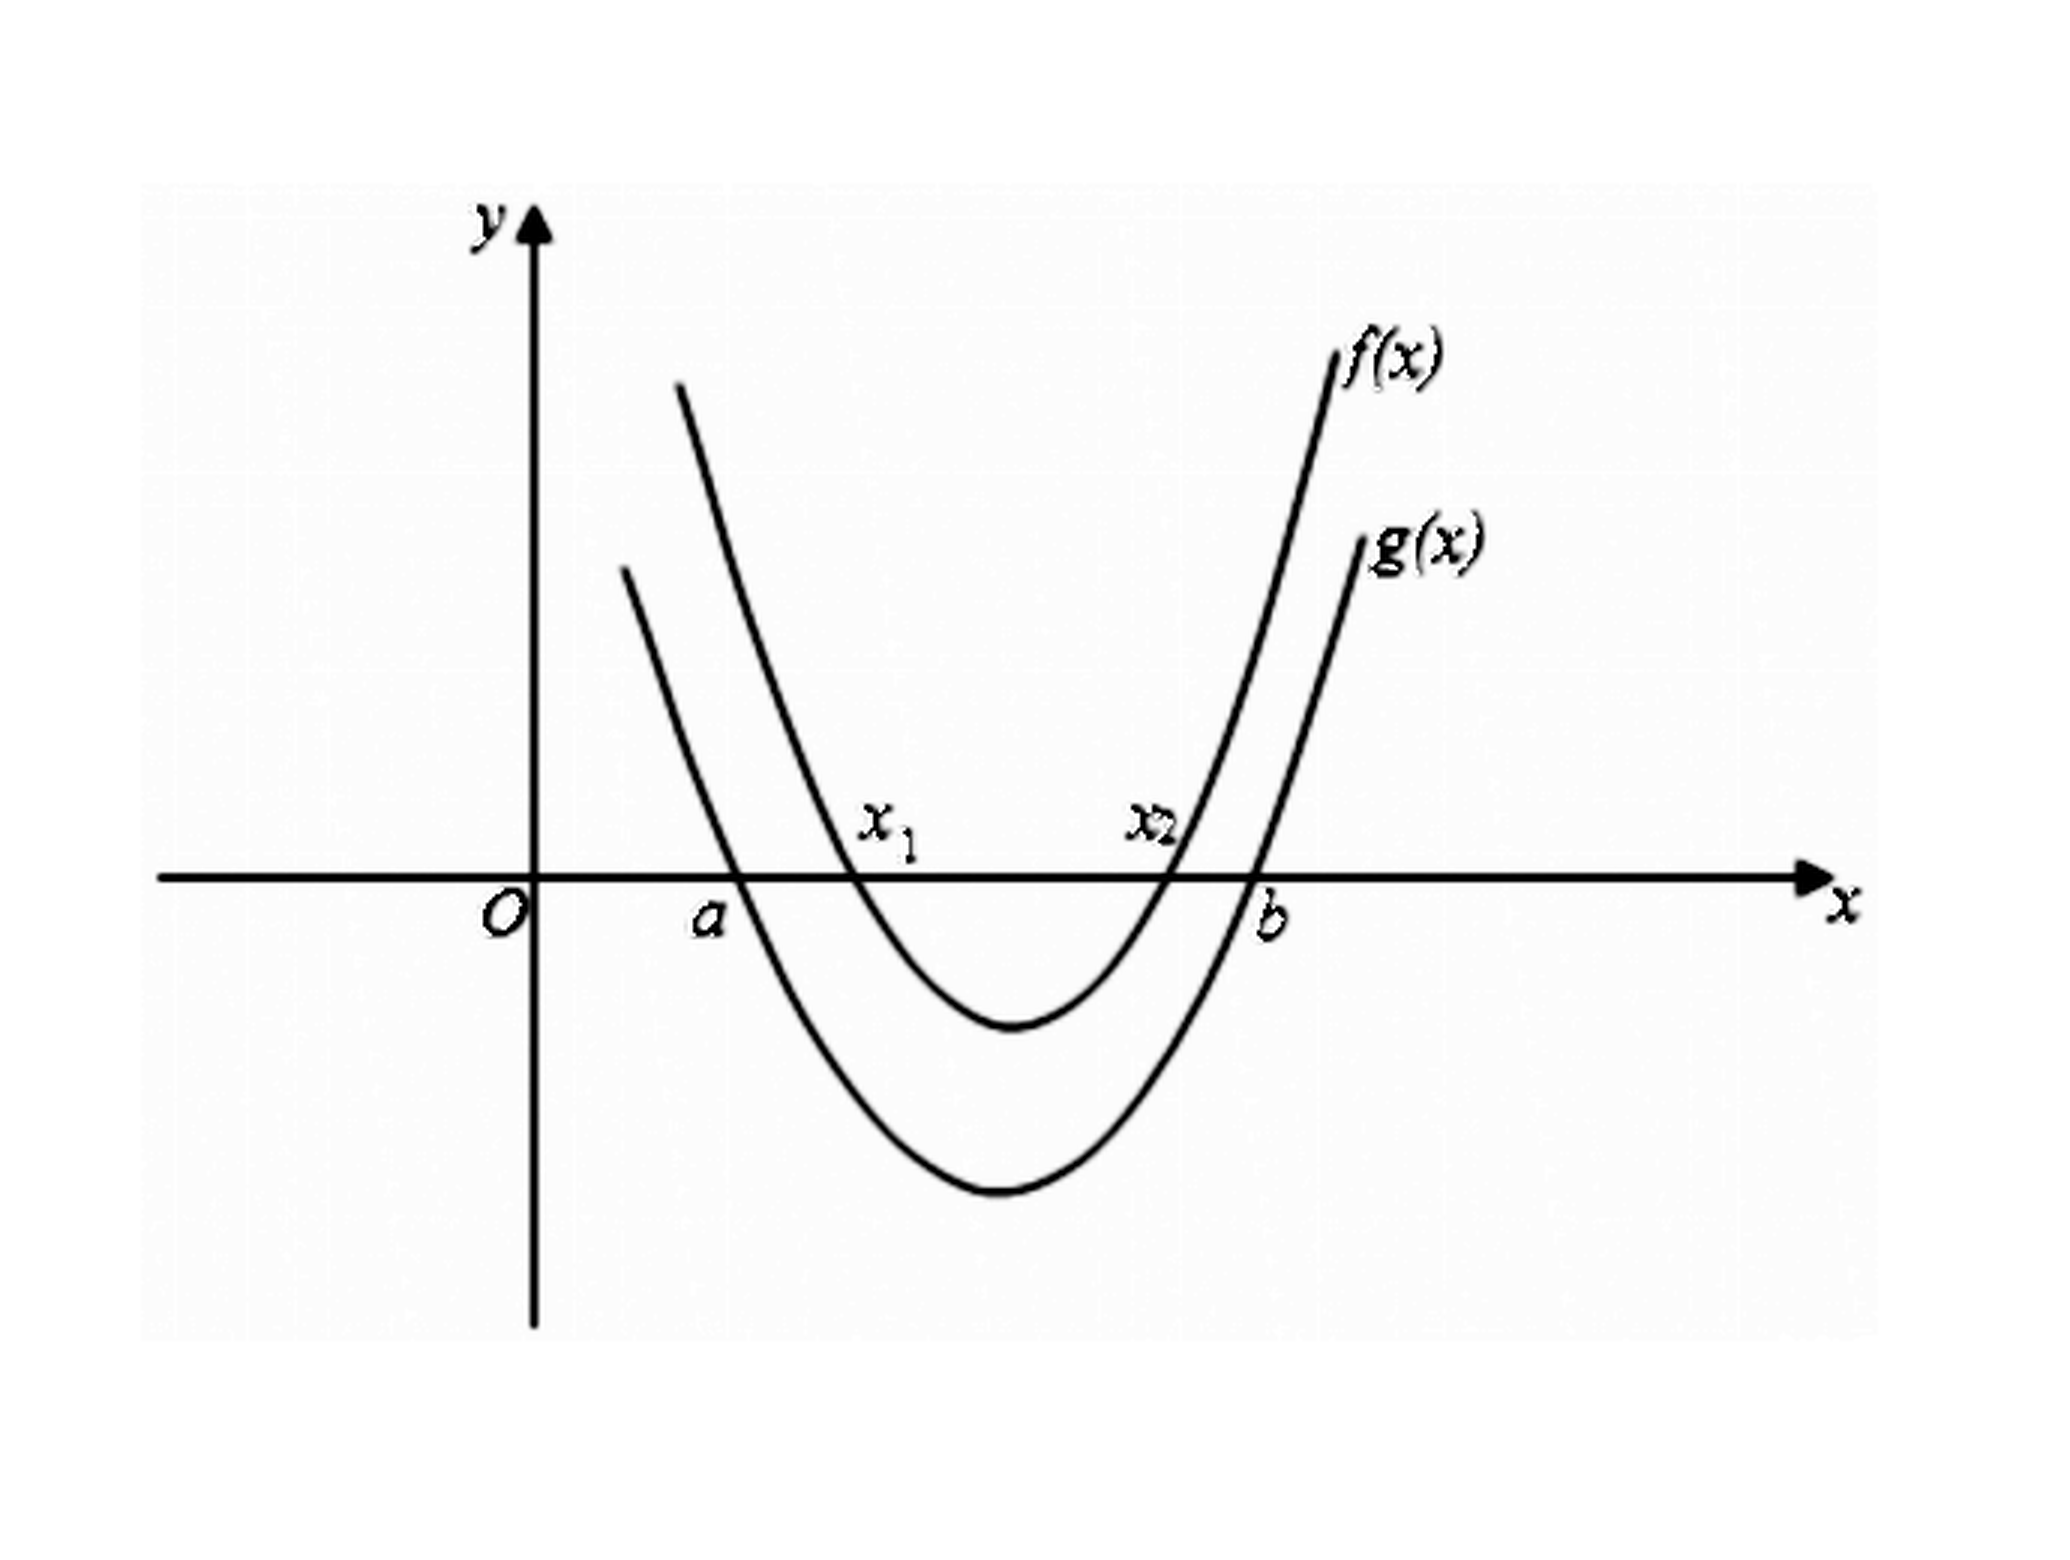
\includegraphics[width=0.52\textwidth]{figures/gao157_q16.png}
\end{center}

\step{由图像得 $a<x_1<x_2<b$，故选 $A$.}
\solend
\fi

\end{enumerate}

\bigsec{三、解答题}

\begin{enumerate}
\setcounter{enumi}{16}

% === Q17 === 解析 6 行；\overline{A}、\varnothing、\subseteq 无、cases
\item 设全集为 $\R$，$m\in\R$，集合 $A=\{x\mid 2<x<5\}$，$B=\{x\mid 2m\leqslant x\leqslant 5m-3\}$.

(1) 若 $m=2$，求 $\overline{A}\cup B$；

(2) 若 $A\cap B=B$，求 $m$ 的取值范围.

\ifanswer
\solbegin
\step{(1) $\overline{A}=\{x\mid x\leqslant2$ 或 $x\geqslant5\}$，当 $m=2$ 时，$B=\{x\mid 4\leqslant x\leqslant7\}$，}
\step{则 $\overline{A}\cup B=\{x\mid x\leqslant2$ 或 $x\geqslant4\}$；}
\step{(2) 因为 $A\cap B=B$，所以 $B$ 是 $A$ 的子集，}
\step{当 $B=\varnothing$ 时，$2m>5m-3$，解得 $m<1$；}
\step{当 $B\ne\varnothing$ 时，$\begin{cases}2m\leqslant5m-3\\2m>2\\5m-3<5\end{cases}$，解得 $1<m<\dfrac85$；}
\step{综上，$m$ 的取值范围是 $(-\infty,1)\cup\left(1,\dfrac85\right)$.}
\solend
\fi

% === Q18 === 解析 2 行；指数式、\lg、换底
\item (1) 设 $a^{2x}=3$，且 $a>0$，求 $\dfrac{a^{3x}+a^{-3x}}{a^x+a^{-x}}$ 的值；

(2) 已知 $\lg2=a, 10^b=3$，用 $a$ 及 $b$ 表示 $\log_{12}25$.

\ifanswer
\solbegin
\step{(1) $\dfrac{a^{3x}+a^{-3x}}{a^x+a^{-x}}=a^{2x}-1+a^{-2x}=3-1+\dfrac13=\dfrac73$；}
\step{(2) $\log_{12}25=\dfrac{\lg25}{\lg12}=\dfrac{2-2\lg2}{2\lg2+\lg3}=\dfrac{2-2a}{2a+b}$.}
\solend
\fi

% === Q19 === 解析 11 行；幂函数、$=0$ 笔误照录、\Delta、\sqrt5、cases
\item 已知幂函数 $f(x)=(m^2+m-1)x^{-2m^2+m+3}$ 在 $(0,+\infty)$ 上为严格增函数.

(1) 求 $f(x)$ 的解析式；

(2) 若 $k+kf(x)>f(x)-x-1$ 对任意实数 $x$ 都成立，求实数 $k$ 的取值范围；

(3) 若关于 $x$ 的不等式 $f(x)\leqslant8x-a$ 的解集中有且仅有 $5$ 个整数，求实数 $a$ 的范围.

\ifanswer
\solbegin
\step{(1) 由题意得 $m^2+m-1=1$，且 $-2m^2+m+3>0$，}
\step{解得 $m=-2$（舍去）或 $m=1$，所以 $f(x)=x^2$；}
\step{(2) $k+kf(x)>f(x)-x-1$ 可化为 $(k-1)x^2+x+k+1=0$ 恒成立，}
\step{当 $k=1$ 时，$x+2>0$，显然不恒成立；}
\step{当 $k\ne1$ 时，要使该二次不等式恒成立，只需 $\begin{cases}k-1>0\\[2pt]\Delta=1-4(k+1)(k-1)\leqslant0\end{cases}$，}
\step{解得 $k\geqslant\dfrac{\sqrt5}{2}$，即所求 $k$ 的范围是 $\left[\dfrac{\sqrt5}{2},+\infty\right)$；}
\step{(3) 不等式 $f(x)\leqslant8x-a$，即 $x^2-8x+a\leqslant0$ 有五个整数解，}
\step{令 $g(x)=x^2-8x+a$，因为该函数开口向上，对称轴为 $x=4$，}
\step{所以解集内的整数为 $2$，$3$，$4$，$5$，$6$，}
\step{由二次函数的性质得，只需 $\begin{cases}g(1)=1-8+a>0\\g(2)=4-8\times2+a\leqslant0\end{cases}$，解得 $7<a\leqslant12$，}
\step{故 $a$ 的取值范围是 $(7,12]$.}
\solend
\fi

% === Q20 === 解析 12 行；材料题、$a+b=1$、大根号、"因出"笔误、分母套分数
\item 问题：正数 $a$、$b$ 满足 $a+b=1$，求 $\dfrac1a+\dfrac2b$ 的最小值.

其中一种解法是：$\dfrac1a+\dfrac2b=\left(\dfrac1a+\dfrac2b\right)(a+b)=1+\dfrac ba+\dfrac{2a}{b}+2\geqslant3+2\sqrt2$，

当且仅当 $\dfrac ba=\dfrac{2a}{b}$ 且 $a+b=1$ 时，即 $a=\sqrt2-1$ 且 $b=2-\sqrt2$ 时取等号.

学习上述解法并解决下列问题：

(1) 若正实数 $x$、$y$ 满足 $x+y=1$，求 $\dfrac2x+\dfrac1y$ 的最小值；

(2) 若实数 $a$、$b$、$x$、$y$ 满足 $\dfrac{x^2}{a^2}-\dfrac{y^2}{b^2}=1$，求证：$a^2-b^2\leqslant(x-y)^2$；

(3) 利用 (2) 的结论，求代数式 $M=\sqrt{2m-5}-\sqrt{m-3}$ 的最小值，并求出使得 $M$ 最小的 $m$ 的值.

\ifanswer
\solbegin
\step{(1) $\dfrac2x+\dfrac1y=(x+y)\left(\dfrac2x+\dfrac1y\right)=3+\dfrac xy+\dfrac{2y}{x}\geqslant3+2\sqrt2$，}
\step{当且仅当 $\dfrac xy=\dfrac{2y}{x}$ 且 $x+y=1$ 时取等号；}
\step{(2) $a^2-b^2=(a^2-b^2)\left(\dfrac{x^2}{a^2}-\dfrac{y^2}{b^2}\right)=x^2+y^2-\left(\dfrac{a^2x^2}{b^2}+\dfrac{b^2y^2}{a^2}\right)$}
\step{$\leqslant x^2+y^2-2\sqrt{\dfrac{a^2x^2}{b^2}\cdot\dfrac{b^2y^2}{a^2}}=x^2+y^2-2xy=(x-y)^2$，}
\step{故当 $b^4x^2=a^4y^2$ 时，等号成立.}
\step{(3) 令 $x=\sqrt{2m-5}, y=\sqrt{m-3}$，由 $\begin{cases}2m-5\geqslant0\\m-3\geqslant0\end{cases}$ 得 $m\geqslant3$，}
\step{$x^2-y^2=(2m-5)-(m-3)=m-2>0$，}
\step{又 $x>0, y>0$，所以 $x>y$，所以 $\dfrac{x^2}{a^2}-\dfrac{y^2}{b^2}=1$，}
\step{由 $x^2-2y^2=1$，得 $\dfrac{x^2}{1}-\dfrac{y^2}{\frac12}=1$，因出 $a^2=1, b^2=\dfrac12$，}
\step{由 (2) 得 $M=\sqrt{2m-5}-\sqrt{m-3}=x-y\geqslant\sqrt{a^2-b^2}=\sqrt{1-\dfrac12}=\dfrac{\sqrt2}{2}$，}
\step{当且仅当 $\dfrac xy=\left(\dfrac ab\right)^2=2$ 取等号，结合 $x^2-2y^2=1$，解得 $x=\sqrt2, y=\dfrac{\sqrt2}{2}$，}
\step{即 $\sqrt{2m-5}=\sqrt2$，得 $m=\dfrac72$，所以 $m=\dfrac72$ 时，$M$ 取得最小值 $\dfrac{\sqrt2}{2}$.}
\solend
\fi

\end{enumerate}

\end{document}
